\documentclass[a4paper, oneside, 12pt, parskip=half, bibliography=totoc,%
               listof=totoc]{scrbook}

% General packages
\usepackage{sourdough}

% Basic attributes
\author{Hendrik Kleinwächter}
\title{The Sourdough Framework}

\begin{document}
\thispagestyle{empty}
\setlength{\unitlength}{1mm}
\noindent\begin{picture}(0,0)(1,-1)
\put(-16.3,-265){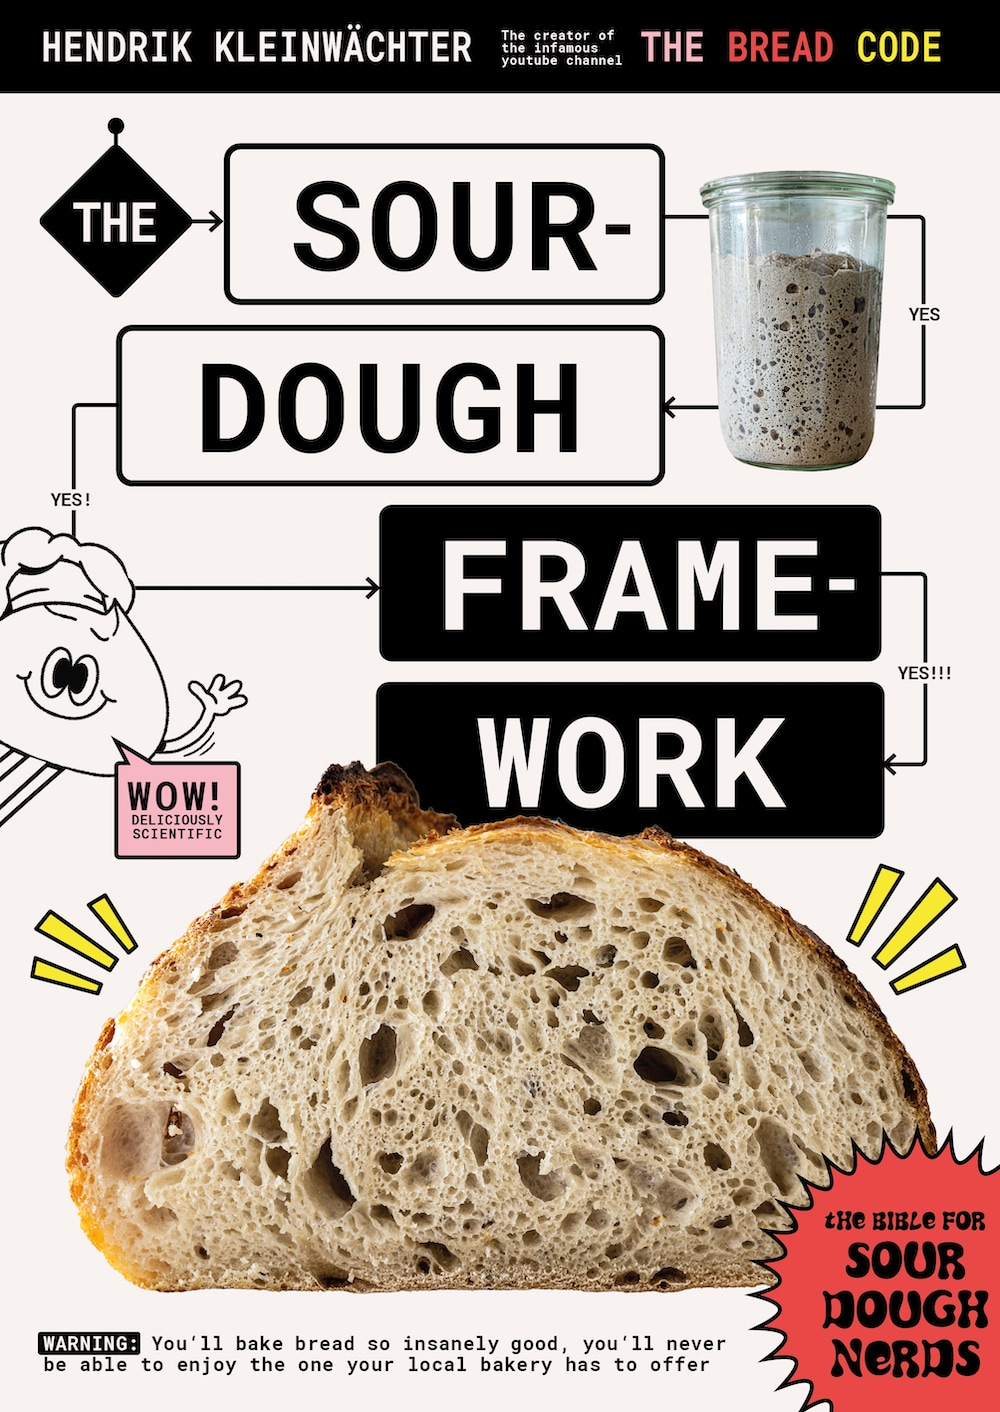
\includegraphics[width=1.33\linewidth]{cover/cover-page.jpg}}
\end{picture}

\newpage
\thispagestyle{empty}

\rule{1pt}{\textheight} % Vertical line
 % Whitespace between the vertical line and title page text
\hspace{0.05\textwidth}
 % Paragraph box for holding the title page text, adjust the width to move the
% title page left or right on the page
%\raggedleft%
\parbox[b]{0.75\textwidth}{%
{\Huge\bfseries The Sourdough Framework}\\[2\baselineskip] % Title
{\large\textit{Version: \today}}\\[4\baselineskip]
{\Large\textsc{Hendrik Kleinwächter}} % Author name, lower case for consistent small caps

% Whitespace between the title block and the copyright text
\vspace{0.5\textheight}

{\noindent The full source code for the book is available at \\
\url{https://github.com/hendricius/the-sourdough-framework/} under CC-BY-SA
license. Do not hesitate to report mistakes or sug\-gestions for
improvements. A hardcover version of the book is also available. More information here:
\url{https://www.breadco.de/hardcover-book}}\\[\baselineskip]
}

\titlepage

\frontmatter
% \tableofcontents
\ifdefined\HCode\else\tableofcontents\fi

\chapter{Foreword}
Hopefully one day there is going to be an awesome foreword
by another break baker!

\chapter{Preface}
If there is one food Germany is known for, it is probably bread.
There are thousands of varieties in Germany,
and making it has been an integral part of our culture.

My bread journey began during childhood. My mother, being a parent
of 3, would always use Saturdays to bake a delicious loaf for the family.
It was a white fluffy sandwich bread, and she made it within one to two hours using store-bought yeast.
Being a bit more experienced, I now realize it's
ideal to wait a little while before cutting into your bread, but back then,
we kids couldn't wait. Mom would cut for us a few slices straight from the oven, and we would
immediately proceed to pour butter or jam on each slice. Within minutes, 1 kg of
flour would be consumed. Bread became an integral part of my weekly food.

I was lucky that my parents could afford a yearly ski trip to
Alto Adige in northern Italy. In the small town called Valdaora, we
would try new restaurants every year, yet always end up in our favorite
pizza place. The pizzas there were incredible. The dough
alone was so tasty that we would order just the bread with a
bit of olive oil and salt.

Of course, my question would always be, ``Mom, can we make this at home, too, please?''
So over the years, we became friends with the owners and would receive
more and more clues as how to make the perfect pizza dough. There
are no secret ingredients inside. It's just flour, water, salt, and a bit of yeast.
How can such a simple combination of ingredients create such an incredibly delicious
pizza dough? My parents, being creatures of habit, would return every year with us,
and every year, my interest would grow. At home, Mom and I attempted to replicate
the recipe. We tried baking on a stone and on a steel. We tried adding oil to the dough and herbs
to the pizza sauce. We fell into an endless cycle of experiments. However, we never managed
to get close to the experience we had while on vacation.

Some years passed, and I eventually began my studies in the small German city of Göttingen.
For the first time, I was faced with shopping for my own bread. It was never
on my mind to actually start baking it for myself. I would just buy 
a good loaf while shopping at the supermarket. My favorite variety
was a Schwarzbrot, Korn an Korn. It’s a very dark and hearty rye bread
with added berries and sunflower seeds. Being a little naïve,
I'd never before examined the packaging of what I was buying. One day, that
changed.

I looked at the label and was shocked. The seemingly
healthy bread consisted of so many other things aside from flour and water.
The black color was not coming from the flour, but from caramelized sugar.
The packaging stated it was a sourdough bread, but then why was there additional yeast?
I thought that if it was really sourdough, it shouldn't require additional yeast, and I
soon realized that something was wrong with the bread I was buying.
I proceeded to check the other supermarket breads, only to discover that they, too,
contained ingredients I'd never heard of. That was the day I lost trust
in supermarket bread.

At home, I decided to research the proper way to make bread, and much to my surprise,
I learned that the recipes for making pizza and bread were actually quite similar, yet
there were also differences. For example, some recipes would call for fresh yeast, while
others would call for dry. Diving deep into various online forums and all their many
discussions, I became even more confused.

I tried using different flours and different brands, all in both organic and non-organic varieties.
I realized then that I knew nothing about making bread. Recipes would often contradict each other,
leaving me further confused. They seemed like little more than a collection of apparently random
steps to follow. The baking instructions and temperatures were all different, too.

Meanwhile, having completed my studies, I started work as an engineer.
We engineers are faced with many challenges. The compiler or runtime is
always screaming at you with errors, and it's your job to figure out how to fix them.
It can take hours, sometimes days, just to fix a simple problem. If you want
to become a software engineer, you have to develop a certain ``never-give-up'' attitude.

When writing code, software engineers often need to use a set of pre-made routines. These routines have been
written by other engineers and can then be used to ship code faster.
This pre-written code is commonly known as {\it a framework}. In many cases,
these frameworks are not built by a single person but by engineers from all around the world,
each of whom can help by improving and changing the source code. Frameworks have made many successful
businesses possible.

In most cases, frameworks do exactly what they claim they do. However,
sometimes you are faced with issues you don't understand. In 99.95 percent
of all software bugs, the developer is the issue. Sometimes, however, the framework has a
bug. That is when the developer must dig deeper to see the 'what' and the 'why' behind what
the framework is doing. You will need to read other engineer's source code, and you will be forced
to understand {\it why} things are happening.

Being unhappy with what I was baking, my engineering mindset took over, and I had
to do my own deep dive to understand what was going on. Much to my surprise, however,
none of the recipes I'd encountered would tell me {\it why} I should use amount X
of water and amount Y of flour, or {\it why} exactly I should use fresh yeast over dry yeast. Why
should I slap my dough while kneading it on the counter? Why is a standmixer
better than kneading by hand?  Why should I let the dough sit for this long?
Why is steaming the dough during baking important? Do I really need to
get myself an expensive Dutch oven to bake bread?

The problem compounded when I started reading about sourdough. It all sounded like black
magic. Why were some sourdoughs made from fruits, while others were made from flour?
Why should one recipe use wheat while another used rye or spelt? How often should the
sourdough be fed? The questions I had then could have filled 20 pages. I was confused,
but I became even more determined to learn how decent bread should be made at home.

The feedback I received from friends helped me to improve with each
iteration of homemade bread. Compared to coding, where you sometimes have to wait months
for this feedback, bread making is much more direct. Plus, you can eat your successes
(and failures!) And, much to my surprise, even those failures started tasting better than
most store-bought breads. Eating a homemade bread that takes you hours to make allows you
to develop a different relationship with your food, and baking bread from scratch with my
bare hands was a welcome change after hours of working on the computer.

I continued learning about the process of fermentation and various techniques of bread making.
I approached the topic of sourdough in a manner similar to software, and after years of
researching and documenting my progress, I decided it was time to share that progress with the
world.

When working on open source projects, it is important to see their history and how the source
code changes over time. This way, you can easily jump back to previous versions. This was
the perfect tool for documenting my recipes, because they, too, would change with each
subsequent iteration. Much to my surprise, my open source work on sourdough was appreciated
by other engineers, and the project became popular on the website GitHub, originally built to
share open source software.

Now, when baking great bread, you also need to learn certain techniques. I figured it would be
easier to share these techniques in video form. Thus, my YouTube channel was born. I chose
the name {\it The Bread Code} to capture my engineering-oriented approach to bread. It took some
time to get right, but after choosing more engaging thumbnails and titles for
the videos I made, the channel started gaining viewers.

Now, three years later, I dedicate two days each week to follow my bread baking passion, while
the other three days I continue to work as a software engineer, writing code on a day-to-day
basis.

My bread days fill me with both joy and passion. To me, there is nothing better than seeing
how many people have made amazing bread thanks to my tips and explanations. The community has
continued to grow, spawning many interesting discussions and ideas surrounding the topic of
bread making. There is always something new to learn, and I feel that even now I am just barely
scratching the surface with what I know and teach. Would you ever have imagined that fruit
flies are like bees and are part of the wild yeast's success story? I made a video where
I tried to cultivate wild yeast spores coming from fruit flies in order
to bake bread. It worked; the bread turned out amazingly well and even tasted good! These kinds of
experiments spark my natural interest. Conducting them and seeing how other people share in my
interest makes me incredibly happy.

The problem with running a YouTube channel is that all the information
you see is filtered and then provided to you through an algorithm. I am concerned
with how algorithms are shaping modern information, because they tend to
put users into certain categories where they will then only see news related to
those same fixed categories. A key metric determining visibility of your channel is how many
people have clicked on a video after it's been shown, and the content you create
is not even shown to every subscriber of your channel. If the algorithm determines the video
is not engaging enough, your content starts to decay in YouTube's nirvana. Even if your video
goes viral, the algorithm will stop showing it once engagement rates with new users goes down,
and older videos fade over time as the decay punishment factor increases. I know, because
I have developed similar algorithms myself as a software engineer.

I've since decided to take some time off from the algorithm cycle to work on something more
long term and meaningful. My mission has always been to share my knowledge with as many people
in the world as possible. That's also why my content has been provided in English rather than
German. After discussions with members of the community, I figured that writing a book could
help me achieve that goal. Most of the books that exist today are collections of recipes. My
idea, however, is to provide you with a deeper foundation of knowledge that you can use to
follow other recipes.

In software terms, this would be a {\it bread framework}.

It is my goal for this book to help everyone facing issues with flour, fermentation, baking,
and more. It should provide a detailed understanding as to why certain steps are necessary
and how to adapt them when things go wrong while making bread.

It is my desire for this knowledge to be accessible to everyone around the world, regardless
of budget, and as such, I do not want to charge for the book. That's why I've decided to make
it open source and have asked the community to support my work financially via my ko-fi page
(https://ko-fi.com/thebreadcode). The community's feedback has been amazing so far, and
I've already raised much more money than initially expected.

The first version of the book will only be available digitally---this way, everyone can read
it---though there might also be a hardcover version in the future, depending on how well received
and appreciated it is by bakers around the world. The hardcover version will, of course, cost a
bit of money, but the digital version will remain free.

In this book, I will try to be as scientific as possible. I in no way claim, however, that
it will itself be a work of science. I have conducted several experiments that I will write
about here, but to truly call this science, you would probably need to repeat the same experiment
a thousand times in a lab environment, which I have not done. I will do my best, however, to provide
scientific references where possible and to clearly distinguish between facts and personal opinion.

I hope you have fun reading this and that you learn more about the fascinating world of bread
making, and it is my sincere wish that this work provides you with the solid toolchain that I wish
I'd had access to when starting my own journey with bread.

Thank you.
Hendrik


\chapter{Acknowledgements}
This book would not have been possible without your help.

With all your donations I have been able to take time off from my job and
focus on this project.

Furthermore many of you have contributed and improved the
instructions, fixed spelling mistakes and/or provided
feedback on the content. Each of you has made this book
better.

By providing this book free of charge,
we can enable more people around the world to bake delicious sourdough
bread at home.

Thank you very much for your support!\\

\begin{filecontents}{supporters.csv}
  \end{filecontents}

  {Big shout-out to all the initial supporters who helped launching this project:}

  \pgfplotstableset{
  begin table=\begin{longtable},
  end table=\end{longtable},
  }

  \pgfplotstabletypeset[col sep=comma,
  header=true,
  columns={Name},
  columns/Name/.style={column type=l,string type},
  every head row/.style={before row=\toprule, after row=\midrule\endhead},
  every last row/.style={after row=\bottomrule}
  ]{supporters.csv}


\mainmatter

\chapter{The history of sourdough}
\chapter{The history of sourdough}%
\label{ch:history}
\begin{quoting}
    We will start this book by briefly talking about the long history of
    sourdough bread from ancient time, and how people used similar process for
    other food like beer. The discovery of yeast and how, together with
    machine development, revolutionized bread making.  More recently
    communities formed around sourdough and home baking, trying to relearn
    lessons from the past.
\end{quoting}

The story of sourdough bread begins in prehistoric oceans. These oceans were the
birthplace of all life on Earth. To better envision the vast history of
our planet, lets create a timeline in one~year/365~days. On this scale,
January~1 signifies Earth's
formation 4.54~billion years ago. Midnight on December~31 is the present.
Each day represents roughly 12~million years. This technique simplifies the
complexity of time but also renders the extraordinary expanse of our planet's
history into a more graspable timeframe. We humans, are in fact a recent
addition to our planet, so young that we made our first appearance on
the evening of December~31.  It seems that humans managed to arrive just
in time to join the celebration at the end of the year.

On March~25, the oceans birthed the first single-celled bacteria. In these
waters, another single-celled life form, \emph{archaea}, also thrived. These
organisms inhabit extreme environments, from boiling vents to icy waters.

\begin{figure}[!htb]
  \centering
  \begin{tikzpicture}
  % Draw horizontal line
  \draw[line width=1pt] (0,0) -- (\textwidth,0);

  % Define the width of each segment
  \pgfmathsetlengthmacro{\segmentwidth}{\textwidth/12}

  % Draw lines for the events, higher up so that they don't overflow the text
  % Placing the lines has been a bit manual work of trying different values
  % Maritime bacteria.

  \draw[line width=1pt] (2.8*\segmentwidth,1) -- (2.8*\segmentwidth,0.2);
  % Eukaryotes
  \draw[line width=1pt] (5.8*\segmentwidth,1.5) -- (5.8*\segmentwidth,0.2);
  % First bacteria on land
  \draw[line width=1pt] (9.1*\segmentwidth,-1.25) -- (9.1*\segmentwidth,-0.2);
  % Maritime fungi ancestors
  \draw[line width=1pt] (9.5*\segmentwidth,-2) -- (9.5*\segmentwidth,-0.2);
  % Fungi on land
  \draw[line width=1pt] (10.8*\segmentwidth,-2.75) -- (10.8*\segmentwidth,-0.2);
  % Yeasts on land
  \draw[line width=1pt] (11.1*\segmentwidth,-3.0) -- (11.1*\segmentwidth,-0.2);
  % First dinosaurs
  \draw[line width=1pt] (11.4*\segmentwidth,1) -- (11.4*\segmentwidth,0.2);
  % Dinosaur extinction
  \draw[line width=1pt] (11.9*\segmentwidth,1.5) -- (11.9*\segmentwidth,0.2);

  % Special lines for december events since they are so close togehter
  \draw[line width=1pt] (12.0*\segmentwidth,3.0) -- (12.0*\segmentwidth,0.2);  % Main branch
  \draw[line width=1pt] (12.0*\segmentwidth,3.0) -- (11.75*\segmentwidth,2.5); % Branch to first humans
  \draw[line width=1pt] (12.0*\segmentwidth,3.0) -- (11.75*\segmentwidth,3.0); % Branch to Jordan
  \draw[line width=1pt] (12.0*\segmentwidth,3.0) -- (11.75*\segmentwidth,3.5); % Branch to Pasteur

  % Draw months and month separators
  \foreach \i/\month in {0/Jan, 1/Feb, 2/Mar, 3/Apr, 4/May, 5/Jun, 6/Jul, 7/Aug, 8/Sep, 9/Oct, 10/Nov, 11/Dec} {
      % Separators
      \draw[line width=1pt] (\i*\segmentwidth,0.1) -- (\i*\segmentwidth,-0.1);
      % Month names
      \node[timeline_event, below] at ({(\i+0.5)*\segmentwidth},-0.1) {\month};
  }
  \draw[line width=1pt] (\textwidth,0.1) -- (\textwidth,-0.1);

  % Place events on the timeline with dates using the timeline_event style
  % As a calculation I used (4.54 billion years / 12 months = 0.3785 billion years/month.
  \node[timeline_event, above] at (2.0*\segmentwidth,1) {Mar 25 - First maritime bacteria and archae};
  \node[timeline_event, above] at (4.50*\segmentwidth,1.5) {June 25 - First organisms with nuklei (eukaryotes)};
  \node[timeline_event, above] at (7.8*\segmentwidth,-1.5) {Oct 4 - First bacteria on land};
  \node[timeline_event, above] at (8.0*\segmentwidth,-2.25) {Oct 15 - First maritime ancestors of fungi};
  \node[timeline_event, above] at (9.7*\segmentwidth,-2.75) {Nov 24 - Fungi on land};
  \node[timeline_event, above] at (10.5*\segmentwidth,-3.25) {Dec 3 - Yeasts on land};
  \node[timeline_event, above] at (10.25*\segmentwidth,1) {Dec 14 - First dinosaurs};
  \node[timeline_event, above] at (10.33*\segmentwidth,1.5) {Dec 29 - Dinosaurs go extinct};
  \node[timeline_event, above, anchor=east, align=right] at (11.75*\segmentwidth,2.5) {Dec 31 - First humans};
  \node[timeline_event, above, anchor=east, align=right] at (11.75*\segmentwidth,3.0) {Dec 31 - Sourdough in Jordan (23:59:55)};
  \node[timeline_event, above, anchor=east, align=right] at (11.75*\segmentwidth,3.5) {Dec 31 - Louis Pasteur isolated yeast (23:59:59)};

\end{tikzpicture}

  \caption[Sourdough microbiology timeline]{Timeline of significant events
    starting from the first day of Earth's existence,
    divided into months, and extending to the present day,
    marked at midnight. This visualization shows the pivotal steps
    of life and sourdough on earth.}%
  \label{fig:planet-timeline}
\end{figure}

Whoever comes first, bacteria or archaea, remains debated. For three
months (or approximately 1.1~billion years), these life forms dominated
the oceans. Then, on June~25 in a highly unlikely event, an archaeon consumed a bacterium.
Instead of digesting it, they formed a symbiotic relationship. This led to the
first nucleated organisms, marking an evolutionary milestone. This event lead
to the development of plants, fungi and also ultimately humans.

Life stayed aquatic for another three months.
On October~4, bacteria first colonized land. By October~15, the
first aquatic fungi appeared. They adapted and, by November~24, had colonized
land.

By December~3, yeasts emerged on land. This laid groundwork for bread-making.
Jump 140~million years to December~14, and dinosaurs arose. Just a couple
of days after their appearance on December~17 the super continent Pangea
started to rift apart, reshaping the continents into their current form.
The dinosaurs reigned until December~29 when they faced extinction.
Another 25~million years later, or our timeline's 2~days after the dinosaur
extinction, humans appeared.

A few hours later after the arrival of humans, a more subtle culinary
revolution was unfolding. By \num{12000}~BC, just 5~seconds before our
metaphorical midnight, the first sourdough breads were being baked in ancient
Jordan. A blink of an eye later, or 4~seconds in our time compression,
Pasteur's groundbreaking work with yeasts set the stage for modern
bread-making. From the moment this book began to take shape to your current
reading, only milliseconds have ticked by~\cite{Yong+2017}.

Now delving deeper into the realm of sourdough, it can likely be traced to aforementioned
Ancient Jordan~\cite{jordan+bread}. Looking at the earth's timeline sourdough
bread can be considered a very recent invention.

\begin{figure}[!htb]
  \centering
  \begin{tikzpicture}
  % Draw horizontal line
  \draw[line width=1pt] (0,0) -- (\textwidth,0);

  % Define the width of each segment
  \pgfmathsetlengthmacro{\segmentwidth}{\textwidth/12}

  % Lines for periods
  \draw[stealth-stealth, line width=1pt] (0,-4.2)
    -- node[midway, timeline_timespan] {Historic breadmaking} ({\segmentwidth * 7.8},-4.2);
  \draw[stealth-stealth, line width=1pt] ({\segmentwidth * 7.8},-4.2)
    -- node[midway, timeline_timespan] {Modern bread} ({\segmentwidth * 12},-4.2);

  % Regularly placed events, not in chronological order
  % since should be placed on top of others on the timeline
  \draw[line width=1pt] ({\segmentwidth*3},1.5) -- ({\segmentwidth*3},0.3)
    node[at start, above, timeline_event] {6000 BC: First beer in Egypt};
  \draw[line width=1pt] ({\segmentwidth*5.95},2.5) -- ({\segmentwidth*5.95},0.3)
    node[at start, above, timeline_event] {70 BC:~First water mill};

  \draw[line width=1pt] ({\segmentwidth*10.50},2.5) -- ({\segmentwidth*10.50},0.3);
  \node[timeline_event, above, anchor=east] at ({\segmentwidth*12.50},2.5) {1950:~Modern Wheat};

  \draw[line width=1pt] ({\segmentwidth*11.20},-3.25) -- ({\segmentwidth*11.20},-0.3);
  \node[timeline_event, above, anchor=east] at ({\segmentwidth*12.20},-3.5) {2020~COVID-19 Pandemic};

    \draw[line width=1pt] ({\segmentwidth*9.60},1.5) -- ({\segmentwidth*9.60},0.3)
    node[at start, above, timeline_event] {1868:~Commercial yeast};
  \draw[line width=1pt] ({\segmentwidth*7.8},0.75) -- ({\segmentwidth*7.8},0.3)
    node[at start, above, timeline_event] {1680:~Discovery of microorganisms};
  \draw[line width=1pt] ({\segmentwidth*9.80},-2.5) -- ({\segmentwidth*9.80},-0.3)
    node[at start, below, timeline_event] {1885:~Electrical mixer};
  \draw[line width=1pt] ({\segmentwidth*9.57},-1.75) -- ({\segmentwidth*9.57},-0.3)
    node[at start, below, timeline_event] {1857:~Isolated Yeast};
  \draw[line width=1pt] ({\segmentwidth*8.80},-1.25) -- ({\segmentwidth*8.80},-0.3)
    node[at start, above, timeline_event] {1785:~Steam mill};

  % Lines to events
  % Cultivation of Einkorn
  \draw[line width=1pt] (0,1) -- (0,0.3);
  \draw[line width=1pt] (0,1) -- (0.25,1);
  \node[timeline_event, above, anchor=west] at (0.25,1) {12000 BC:~Cultivation of Einkorn};

  % Sourdough in Jordan
  \draw[line width=1pt] (0,-1) -- (0,-0.3);
  \draw[line width=1pt] (0,-1) -- (0.25,-1);
  \node[timeline_event, above, anchor=west] at (0.25,-1) {12000 BC:~Sourdough in Jordan};
  % Events

  % Indicators for period
  % Draw months and month separators
  \foreach \i/\month in {0/12000, 1/10000, 2/8000, 3/6000, 4/4000, 5/2000,
  6/0, 7/1600, 8/1700, 9/1800, 10/1900, 11/2000, 12/2100} {
      % Separators
      \draw[line width=1pt] (\i*\segmentwidth,0.1) -- (\i*\segmentwidth,-0.1);
      % Events for timeline
      \node[timeline_event, below] at ({(\i)*\segmentwidth},-0.1) {\month};
  }
\end{tikzpicture}

  \caption[Sourdough history timeline]{Timeline of significant discoveries and
  events leading to modern sourdough bread.}%
  \label{fig:sourdough-timeline}
\end{figure}

The exact origins of fermented
bread are, however, unknown. One of the most ancient preserved
sourdough breads has been excavated in Switzerland~\cite{switzerland+bread}.

\begin{figure}[ht]
  \centering
  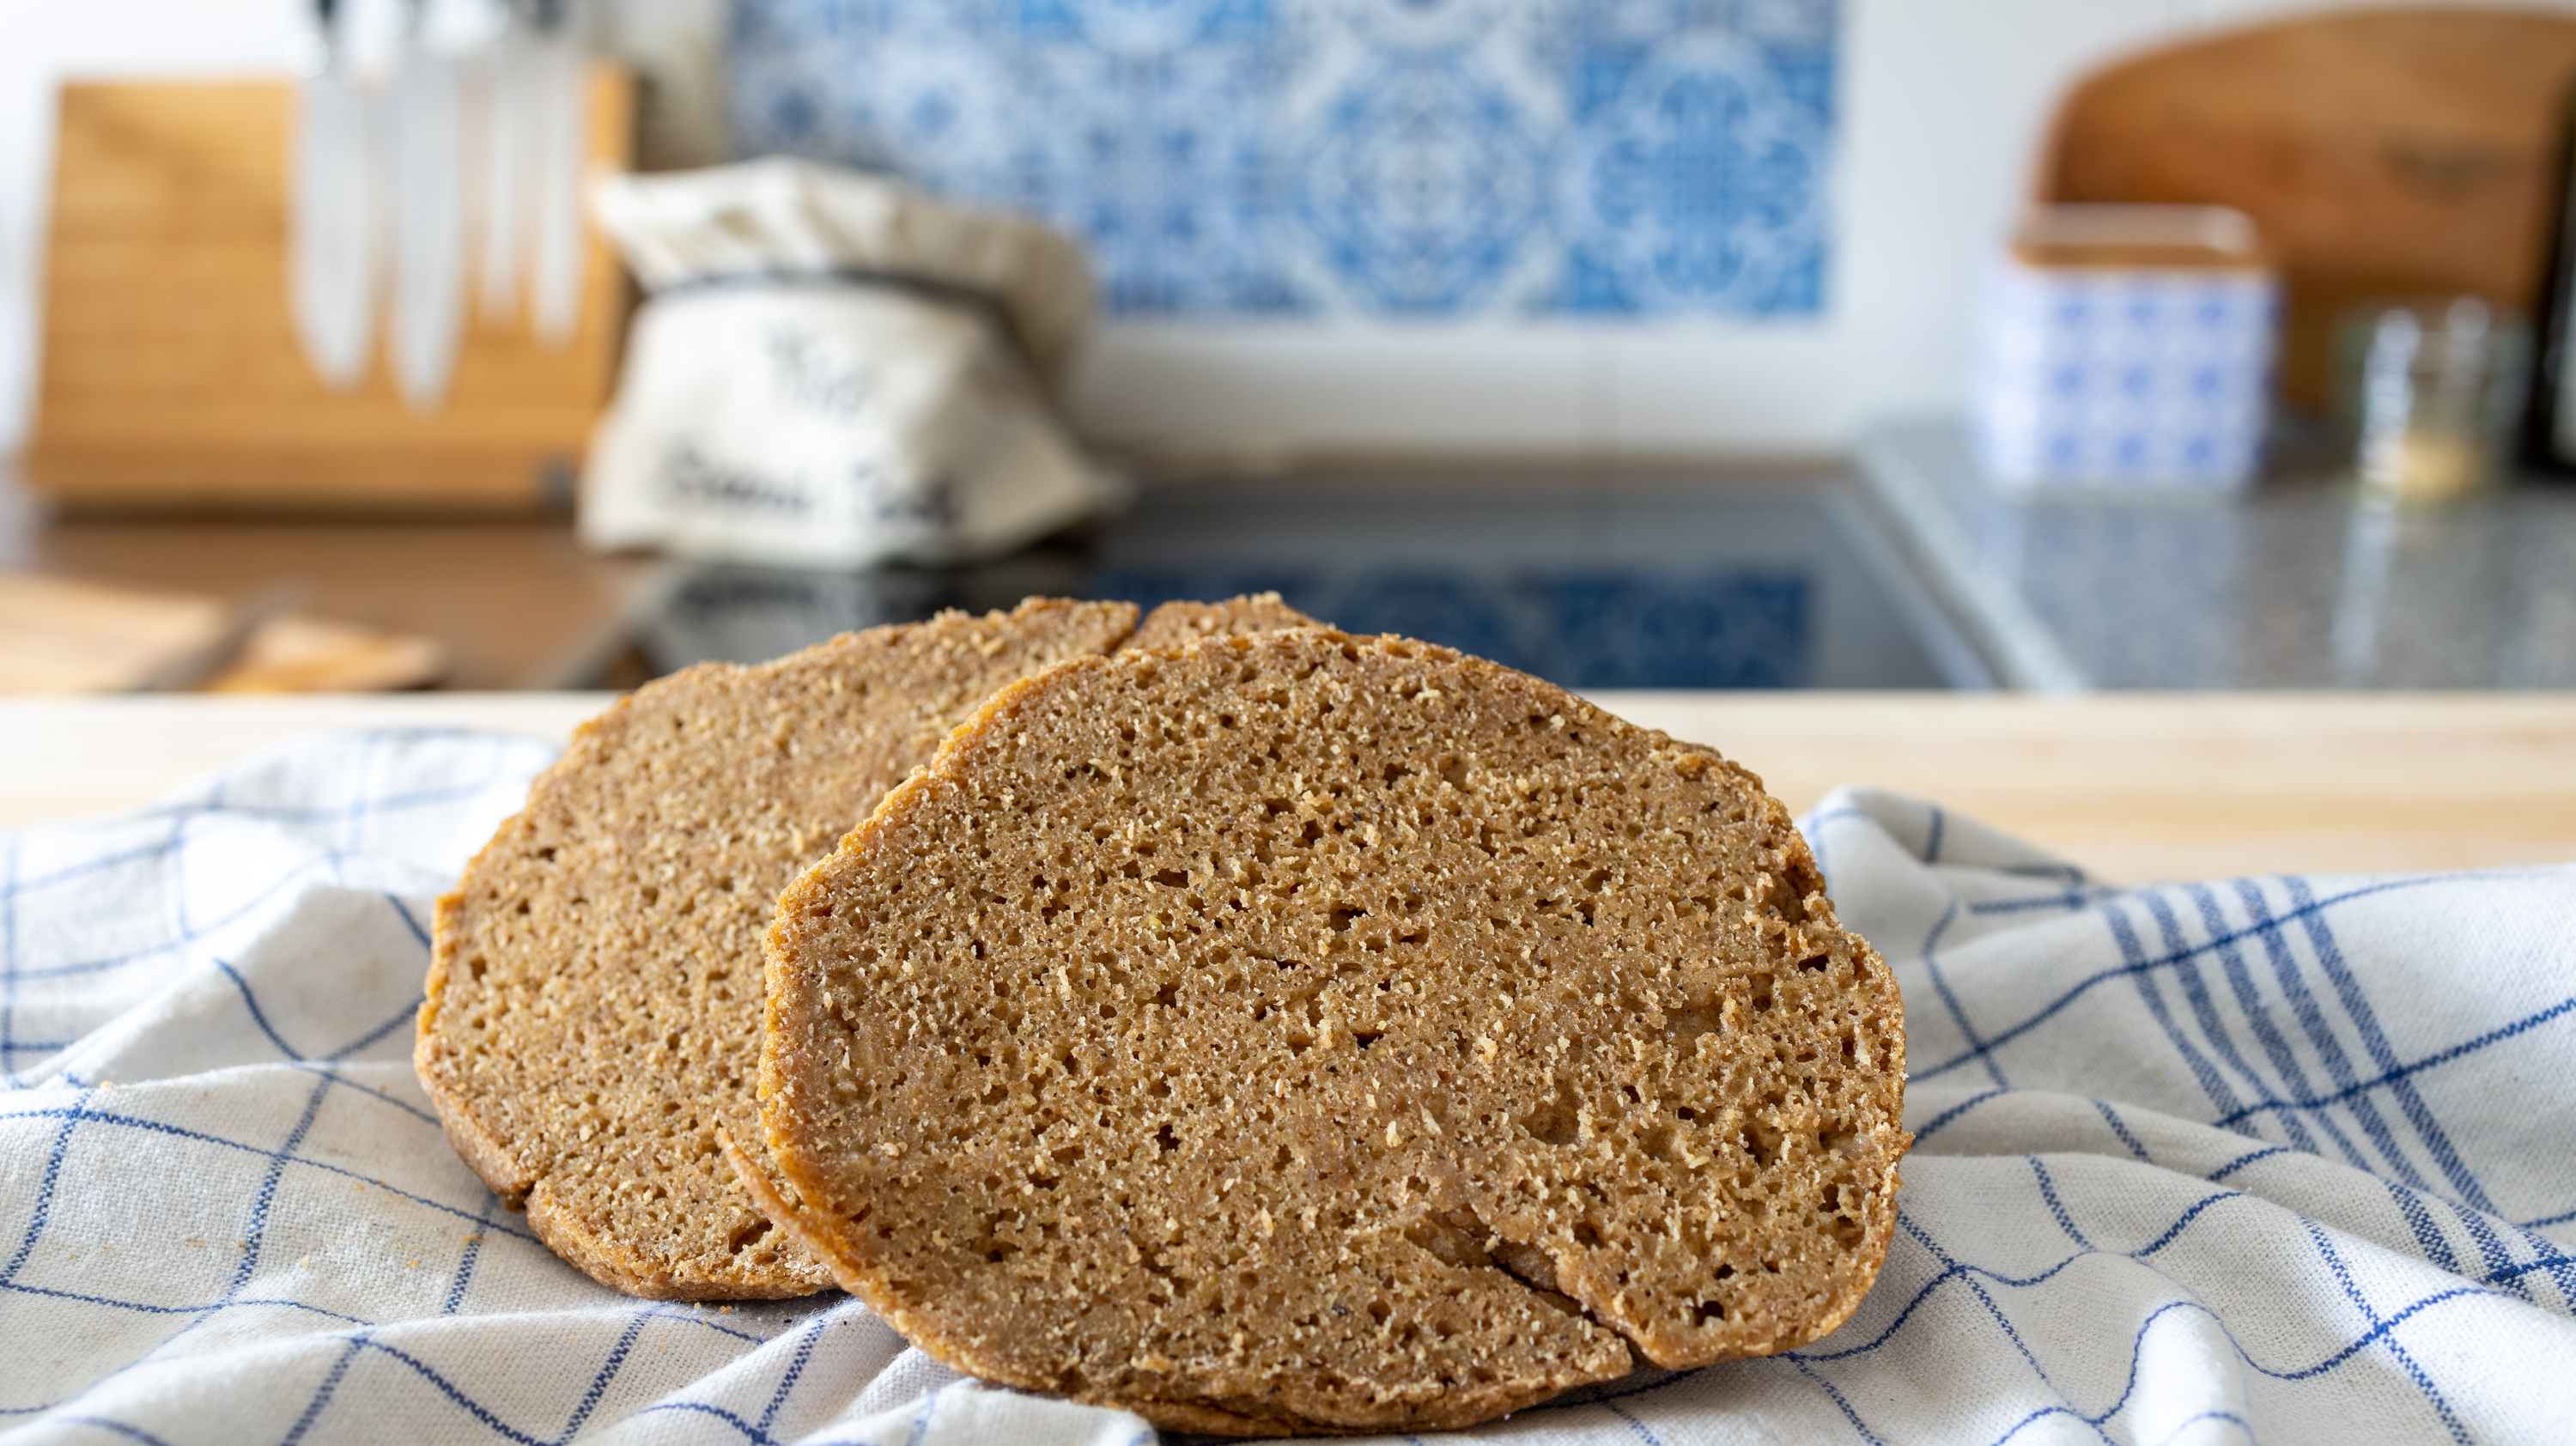
\includegraphics[width=\textwidth]{einkorn-crumb}
  \caption[Ancient Einkorn flatbread]{An ancient Einkorn flatbread. Note the
      dense crumb structure.}%
  \label{fig:einkorn-crumb}
\end{figure}

Another popular story is that a lady in Egypt was making
a bread dough close to the Nile river. The lady forgot the
dough and at her return a few days later, she noticed that the dough had
increased in size and smelled funky. She decided to bake
the dough anyway and was rewarded with a much
lighter, softer, better tasting bread dough. From that day
on she continued to make bread this way~\cite{egyptian+bread}.

Little did the people back then know that tiny microorganisms
were the reason the bread was better. It is not clear when
they started using a bit of the dough from the previous
day for the next batch of dough. But by doing so, sourdough
bread making---as we know it today---was born: Wild yeast
in the flour and in the air, with bacteria
starting to decompose the flour-water mixture.
The yeast makes the dough fluffy,
and the bacteria primarily creates acidity. The different
microorganisms work in a symbiotic relationship. Humans
appreciated the enhanced airy structure and slight acidity
of the dough. Furthermore, the shelf life of such bread
was extended due to the increased acidity.

Quickly, similar processes were discovered when brewing beer
or making wine. A small tiny batch of the previous production
would be used for the next production. In this way, humans created
modern bread yeasts, wine yeasts, and beer yeasts~\cite{egypt+beer}.

Over time with each batch, the yeasts and bacteria
would become better at consuming whatever they were thrown at.
By feeding your sourdough starter, you are selectively breeding
microorganisms that are good at eating your flour. With
each iteration, your sourdough knows how to better ferment the flour
at hand. This is also the reason\footnote{It is crazy if you think about it.
People have been using this process despite not knowing what was going on for
thousands of years!} why more mature sourdough starters sometimes tend to
leaven doughs faster~\cite{review+of+sourdough+starters}.  The sourdough in
itself is a symbiotic relationship, but the sourdough
also adapted to humans and formed a symbiotic relationship with us.
For food and water, we are rewarded with delicious bread. In exchange,
we shelter and protect the sourdough. Spores from the starter
are spread through aerial contamination or insects like fruit flies.
This allows the sourdough starter to spread its spores even
further all around the world.

Evidence suggests early grain grinding in northern Australia around
\num{60000}~BC, notably at the Madjedbebe rock shelter in Arnhem
Land~\cite{aboriginal+grinding+stones}.  However, a more significant
advancement occurred later, as documented by the ancient Greek geographer
Strabo in \num{71}~BC\@.  Strabo's writings described the first water-powered
stone mill, known as a \emph{gristmill}. These mills advanced flour production
from a few kilograms up to several metric tons per day~\cite{history+mills}.

These early mills featured horizontal paddle wheels, eventually termed
\emph{Norse wheels} due to their prevalence in Scandinavia.  The paddle wheels
connected to a shaft, which, in turn, linked to the central runner stone for
grinding. Water flow propelled the paddle wheels, transferring the grinding
force to the stationary \emph{bed}, typically a stone of similar size and
shape. This design was straightforward, avoiding the need for gears. However,
it had a limitation: the stone's rotation speed relied on water volume and
flow rate, making it most suitable for regions with fast-flowing streams,
often found in mountainous areas~\cite{mills+scandinavia}.

In the year \num{1680}, a remarkable scientist by the name of
Antonie~van~Leeuwenhoek introduced a groundbreaking innovation that would
forever alter our understanding of the microscopic world and ultimately bread
making.  Van~Leeuwenhoek, a master of lens craftsmanship, possessed an
insatiable fascination with realms invisible to the naked eye. His pioneering
work birthed the first modern microscope.  What set Van~Leeuwenhoek apart was
the exceptional quality of his lenses, capable of magnifying tiny
microorganisms by an astounding factor of \num{270}.  Driven by an unrelenting
curiosity to unveil the unseen, he embarked on a journey of exploration. He
scrutinized flies, examined lice-infested hair, and ultimately turned his gaze
toward the tranquil waters of a small lake near Delft.

In this serene aquatic habitat, he made astonishing observations, discovering
algae and minuscule, dancing creatures hitherto hidden from human perception.
Eager to share his revelatory findings with the scientific community,
Van~Leeuwenhoek faced skepticism, as it was difficult to fathom that someone
had witnessed thousands of diminutive, dancing entities—entities so tiny that
they eluded the human eye.

Undeterred by skepticism, he continued his relentless pursuit of the unseen,
directing his lens towards a brewer's beer sludge. In this obscure medium,
Van~Leeuwenhoek made history by becoming the first human to lay eyes upon
bacteria and yeast, unraveling a previously concealed world that would
revolutionize our understanding of microbiology~\cite{Yong+2017+Leeuwen}.

At the same time brewers would start to experiment with utilizing the muddy
leftovers of the beer fermentation to start making doughs. They would notice
that the resulting bread doughs were becoming fluffy and compared
to the sourdough process would lack the acidity in the final product.
A popular example is shown in a report from \num{1875}. Eben Norton Horsford
wrote about the famous \emph{Kaiser Semmeln} (Emperor's bread rolls).
These are essentially bread rolls made with brewer's yeast instead
of the sourdough leavening agent. As the process is more expensive,
bread rolls like these were ultimately consumed by the noble people
in Vienna~\cite{vienna+breadrolls}.

Industrialization of the grist milling process, starting in the late
18\textsuperscript{th}~century with Oliver Evans (\num{1785}) and his mill
designs for continuous hands-off flour production~\cite{evans+mill}, and
evolving to steam-powered mills, made possible significant advancements in
bread production.

\begin{figure}[ht]
  \centering
  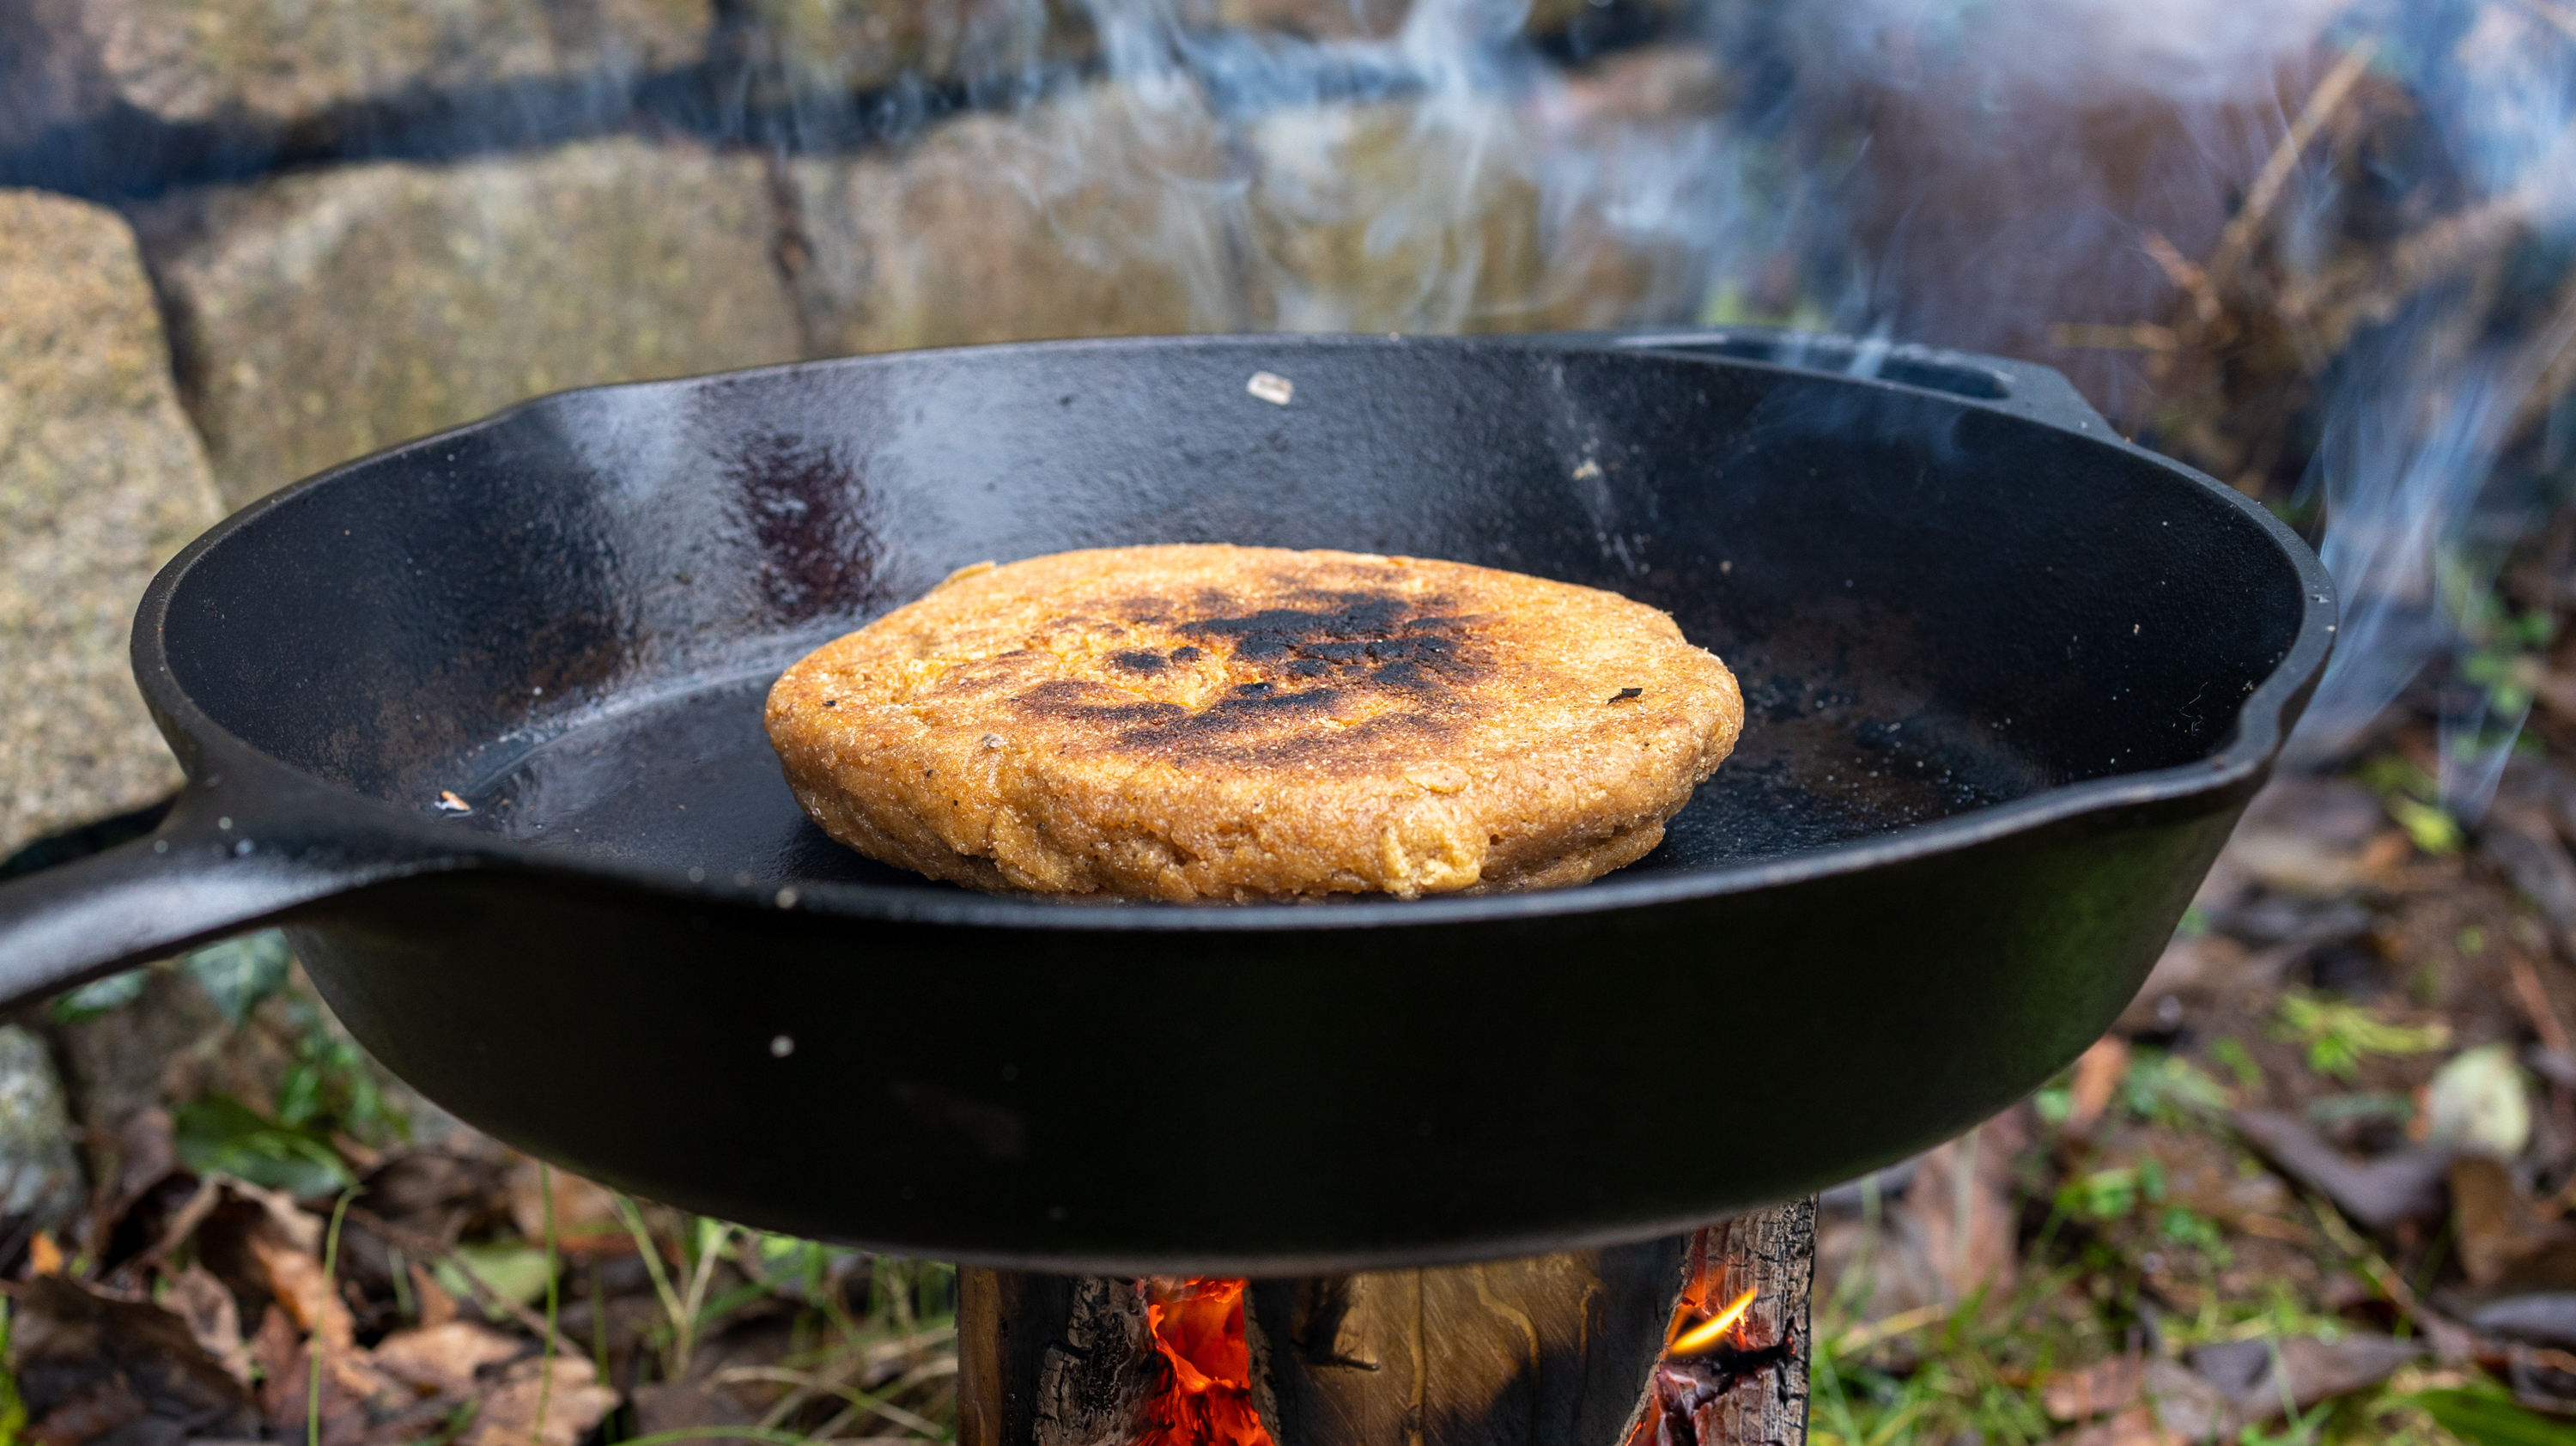
\includegraphics[width=\textwidth]{sourdough-stove}
  \caption{A bread made over the stove without an oven.}%
  \label{fig:sourdough-stove}
\end{figure}

The biggest advancement of industrial bread making happened in \num{1857}.
The French microbiologist Louis Pasteur discovered the process of alcoholic
fermentation. He would prove that yeast microorganisms are the reason for
alcoholic fermentation and not other chemical catalysts. He continued with his
research and was the first person to isolate and grow pure yeast strains.
Soon later in \num{1868} the Fleischmann brothers Charles and Maximilian were
the first to patent pure yeast strains for bread making. The yeasts offered
were isolated from batches of sourdough. By \num{1879} the machinery was built
to multiply the yeast in large centrifuges~\cite{fleischmann+history}.  The
pure yeast would prove to be excellent and turbocharged at leavening bread
doughs. What would previously take 10~hours to leaven a bread dough could now
be done within 1~hour.  The process became much more efficient. What
ultimately made making large batches of dough possible, was the invention of
the electrical kneader.  Rufus Eastman, an American inventor, is often
credited with an important advancement in mixer technology. In \num{1885}, he
received a patent for an electric mixer with a mechanical hand-crank
mechanism.  This device was not as advanced or as widely adopted as later
electric mixers, but it was an early attempt to mechanize mixing and kneading
processes in the kitchen using electricity.  Eastman's invention represented
an important step in the development of electric mixers, but it wasn't as
sophisticated or popular as later models like the KitchenAid mixer. The
KitchenAid mixer, introduced in \num{1919}, is often recognized as one of the
first widely successful electric mixers and played a significant role in
revolutionizing kitchen appliances for home
cooks~\cite{first+mixer}~\cite{kitchenaid+history}.

During World~War~II the first packaged dry yeast was developed. This would
ultimately allow bakeries and home bakers to make bread much faster and more
consistently. Thanks to pure yeast, building industrial bread making machines
was now possible. Provided you maintain the same temperature, same flour and
yeast strains fermentation became precisely reproducible. This ultimately lead
to the development of giga bakeries and flour blenders. The bakeries demanded
the same flour from year to year to bake bread in their machines.  For this
reason, none of the supermarket flour you buy today is single origin.  It is
always blended to achieve exactly the same product throughout the years.

Modern wheat, specifically the high-yielding and disease-resistant varieties
commonly grown today, began to be developed in the mid-20\textsuperscript{th}
century. This period is often referred to as the \emph{Green Revolution.}

One of the key figures in this development was American scientist Norman
Borlaug, who is credited with breeding high-yield wheat varieties,
particularly dwarf wheat varieties, that were resistant to diseases and could
thrive in various environmental conditions. His work, which started in the
1940s and continued through the \num{1960}s, played a crucial role in
increasing wheat production worldwide and alleviating food
shortages~\cite{green+revolution}.

As fermentation
times sped up, the taste of the final bread would deteriorate.
The sprouting process induced by certain enzymes is essential
to developing a fluffier texture and better tasting crust. This
can't be indefinitely sped up. Soon bakeries would start
to introduce additional enzymes to achieve similar properties
to sourdough bread in yeast-based doughs. Sourdough almost completely
vanished from the surface of the Earth. Only a handful
of true nerds would continue making bread with sourdough.

Suddenly people started to talk more often about celiac disease
and the role of gluten. The disease isn't new; it has first
been described in \num{250}~AD~\cite{coeliac+disease}. People
would note how modern bread has much more gluten compared
to ancient bread. The bread in ancient times probably was much flatter.
The grains over time have been bred more and more towards containing a higher
amount of gluten. Gluten is a protein that gives modern
bread its typical soft fluffy crumb structure. The
gluten proteins bind together once activated with water.
Throughout the course of the fermentation, \ch{CO2} is trapped
in this protein matrix. The tiny created chambers expand
during the baking process. As the dough gelatinizes while
being heated, the structure is fortified. This makes the bread appear
soft and fluffy when tasting it. Similar to drinking raw cow's milk,
your immune system might react to the consumed proteins.
There is gluten intolerance
and celiac disease. When people say they don't handle
gluten well, it's mostly a gluten intolerance they describe.
Some people describe similar issues when consuming
too much lactose. If you eat a long-fermented cheese
however, most of the lactose has been fermented by
the tiny microorganisms. People would investigate and
note how sourdough bread can typically be handled better
compared to plain, fast-made factory bread. The
reason for this is that enzymes take time to work the dough.
Gluten is a storage protein of flour. Once
sprouting is activated by adding water, the protease
enzyme starts to convert the gluten into tinier amino acids
that are required for sprouting. Over time you are effectively
losing gluten as it's naturally broken down. Furthermore,
traditionally lactic acid bacteria would start to decompose
the flour-water mix. Almost everything is recycled in nature.
Part of their diet is to consume the proteins in the dough.
Modern bread is faster and no longer has lactic acid bacteria.
Both factors together mean that you are consuming products
with a much higher gluten value compared to ancient times
when natural fermentation was used~\cite{raffaella+di+cagno}.

During the California Gold Rush, French bakers brought the sourdough
culture to Northern America. A popular bread became the
San Francisco sourdough. It's characterized by its unique
tang (which was previously common for every bread). It
however remained more of a niche food while industrial bread
was on the rise. What really expedited
the comeback of sourdough was the \num{2020} COVID-19 pandemic.
Flour and yeast became scarce in the supermarkets. While
flour returned yeast couldn't be found. People started
to look for alternatives and rediscovered the ancient
way of making sourdough bread. Soon many realized
that making sourdough bread is more complex than modern
yeast-based bread. You need to maintain a sourdough starter
and have it in ideal shape to properly ferment your dough.
Furthermore, compared to a yeast-based dough, you can't just
punch the dough down and let the fermentation continue.
You can overferment your dough, resulting in a sticky
dough mess. This complexity led to many bakers looking
for help and many thriving communities formed around
the topic of homemade bread.

When interviewing Karl de~Smedt (owner of the Sourdough
Library) he said something that changed my way of thinking
about bread: ``The future of
modern bread is in the past~\cite{interview+karl+de+smedt}.''


\chapter{How sourdough works}
In this chapter, we will cover the basics of how sourdough ferments.
First, we will look at the enzymatic reactions that take place
in your flour the moment you add water, triggering the fermentation
process. Then, in order to better understand this process, we will
learn more about the yeast and bacterial microorganisms involved.

\begin{figure}[!htb]
  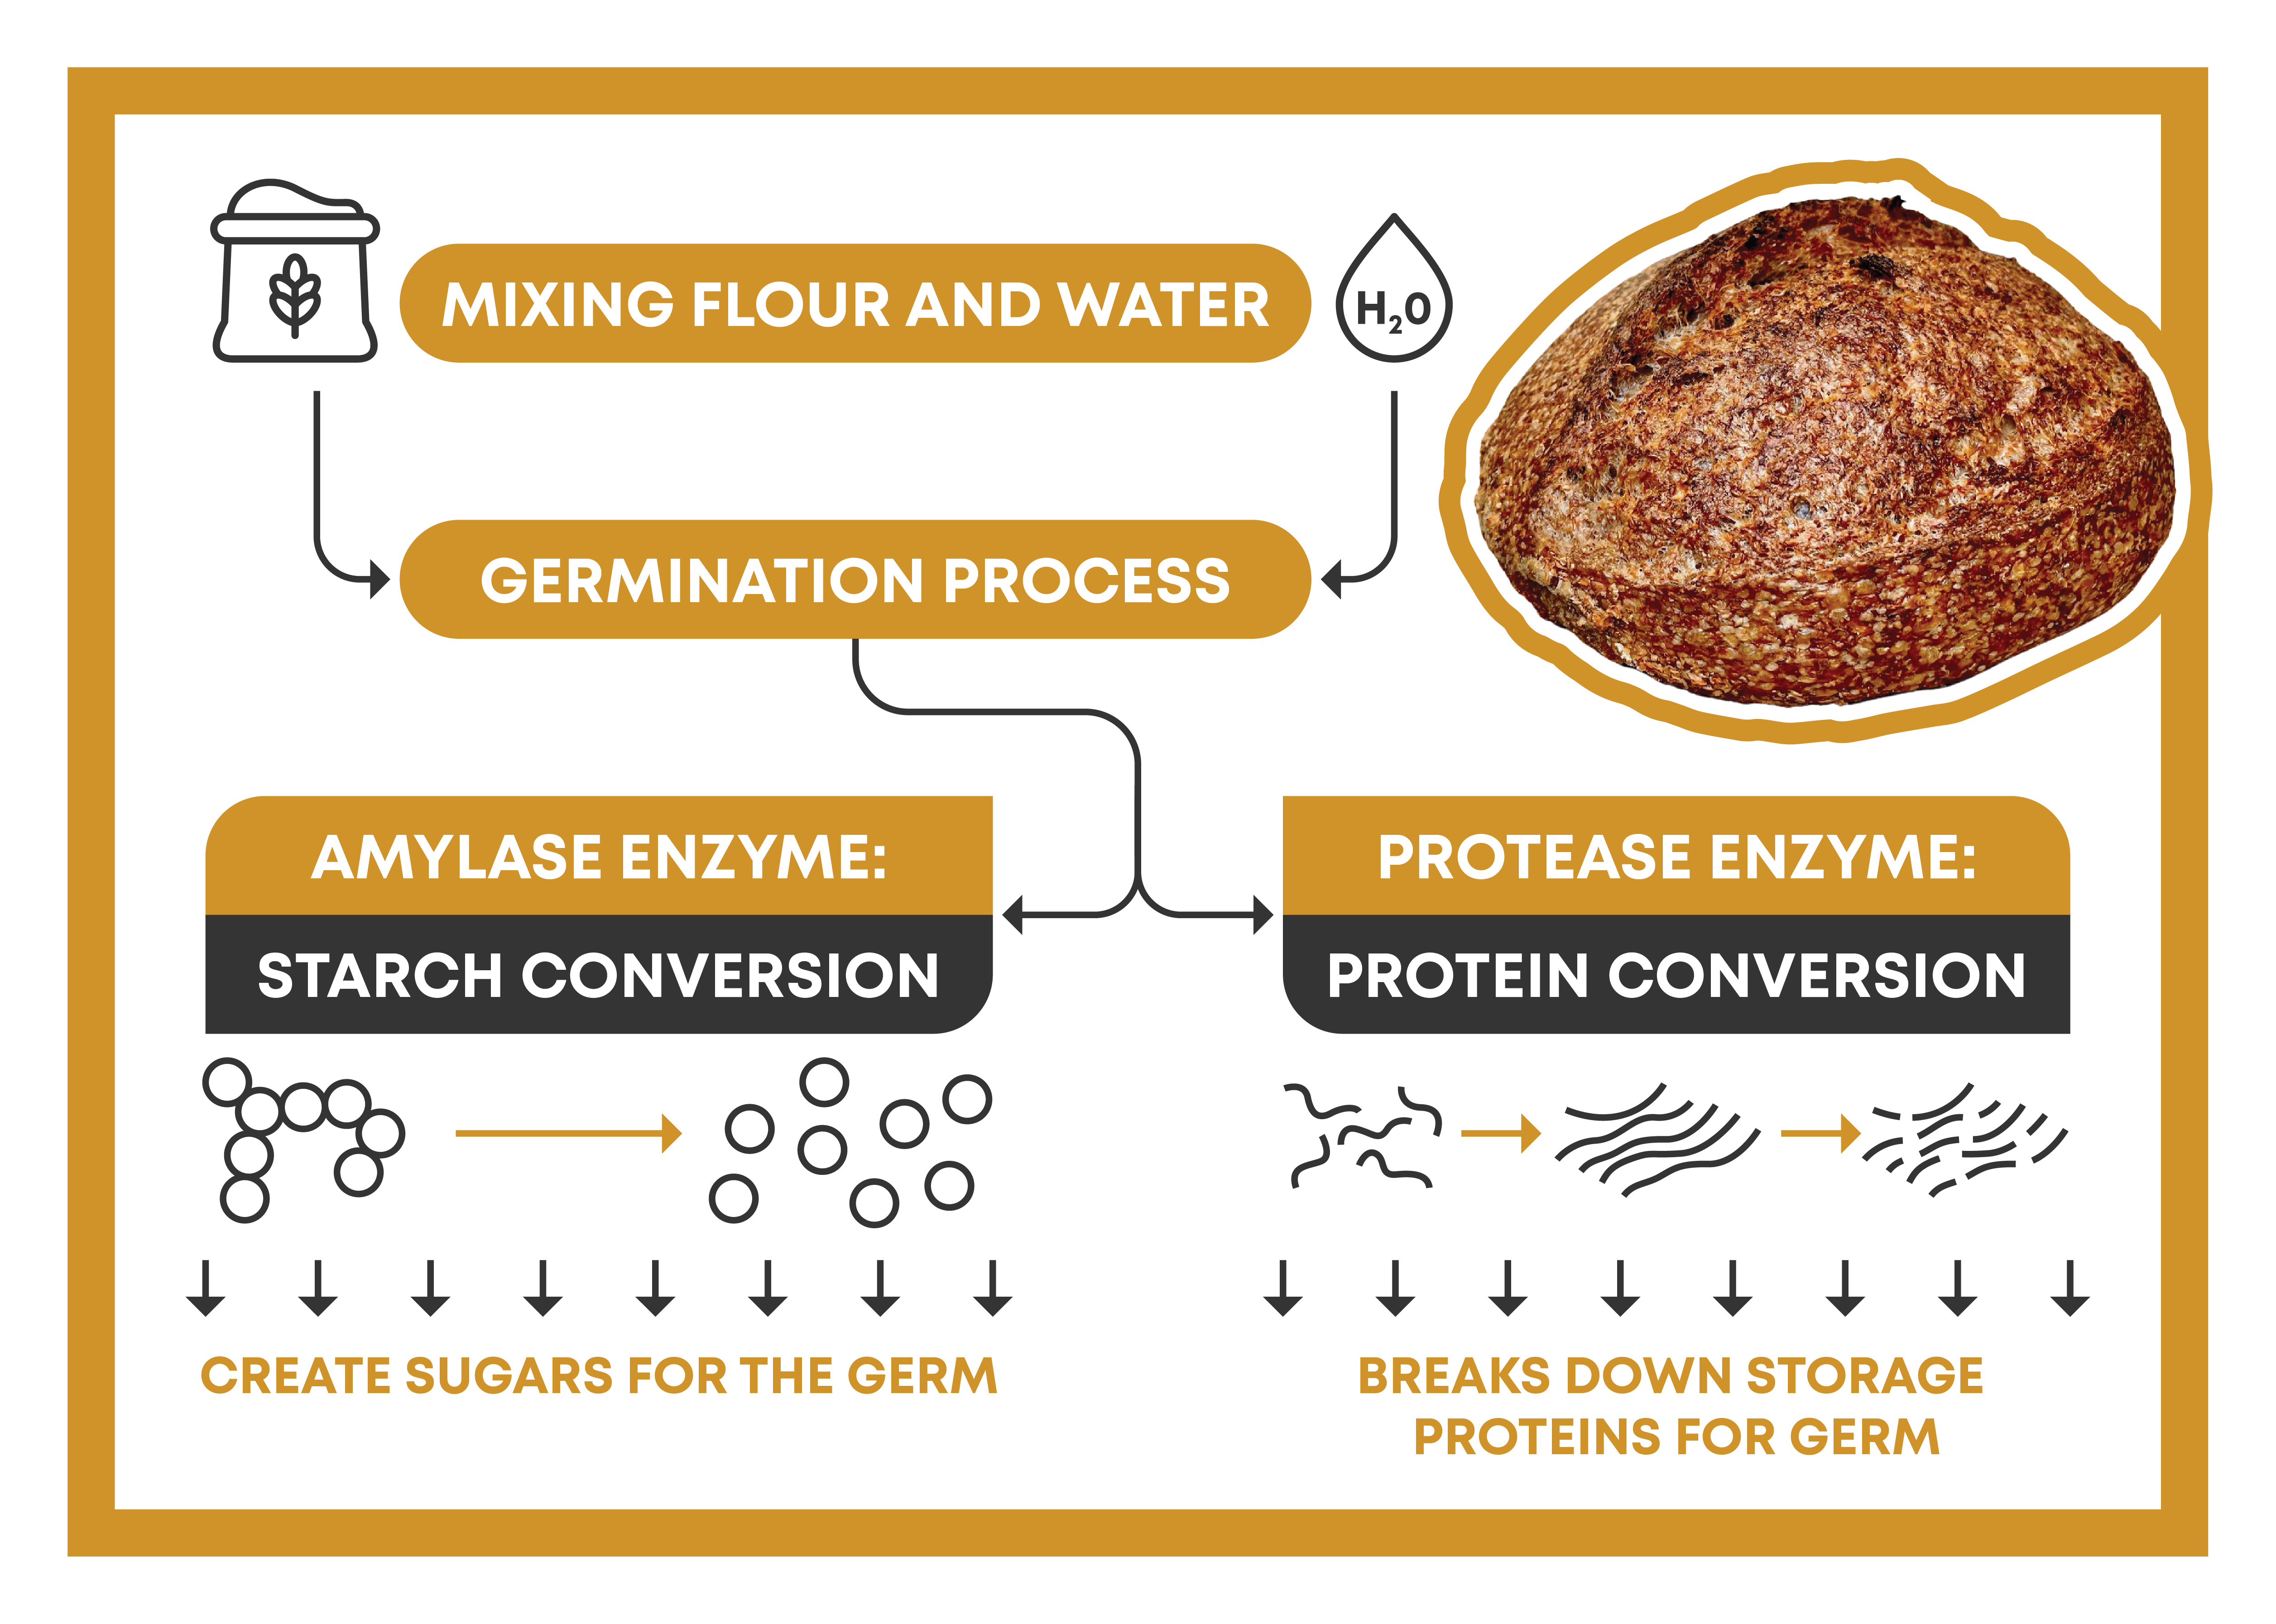
\includegraphics[width=\textwidth]{infographic-enzymes}
  \caption{How amylases and proteases interact with flour}
  \label{infographic-enzymes}
\end{figure}

\section{Enzymatic reactions}

To understand the many enzymatic reactions that take place when flour
and water are mixed, we must first understand seeds and their role in
the lifecycle of wheat and other grains.

Seeds are the primary means by which many plants, including wheat,
reproduce. Each seed contains the embryo of another plant, and must
therefore contain all the nutrients that new plant requires to grow.

When the seed is dry, it is in hibernation mode and can sometimes be
stored for several years. The moment it comes into contact with water,
however, it begins to sprout. The seed turns into a germ, requiring the
stored nutrients to be converted into something the plant can use while
it grows. The catalyst that makes the associated reactions possible is water.

The seed typically contains the first prototypical leaves of the plant,
and can put down roots using the stored nutrients inside. Once those leaves
break through the soil and come into contact with the sunlight above, they
begin to photosynthesize. This process is the plant's engine, and with the
energy photosynthesis produces, the plant can continue to grow more roots,
enabling it to access additional nutrients from the soil. These additional
nutrients allow the plant to grow more leaves, increasing its photosynthetic
activity so that it can thrive in its new environment.

Of course, a ground flour can no longer sprout. But the enzymes that
trigger this process are still present. That's why it's important not to
mill grains at too high a temperature, as doing so could damage some of
these enzymes.

Normally, the grain seed shields the germ against pathogens. However, as the
grain is ground into flour, the contents of the seed are exposed. This is ideal
for our sourdough microorganisms.

% I removed the line referencing yeast as a saprotrophic fungus since you
% cover this later on in the chapter and removing that helps the text to
% flow more smoothly.
Neither the yeast nor the bacteria can prepare their own food. However, as
the enzymes are activated, the food they need becomes available, allowing them
to feed and multiply.

The two main enzymes involved in this process are \textbf{amylase} and
\textbf{protease}. For reasons that will soon be clear, they are of the utmost
importance to the home baker, and their role in the making of sourdough is a
key puzzle piece to making better-tasting bread.

\subsection{Amylase}

Sometimes, when you chew on a potato or a piece of bread for a long period
of time, you'll perceive a sweet flavor on your tongue. That's because your
salivary glands produce amylase. Amylase breaks down complex starch molecules
into easily-digestible sugars. The germ needs this to produce more plant
matter, and your body needs this to kick-start the digestive process. Normally,
the microorganisms on the surface of the grain can't consume the freed maltose
molecules, which remain hidden inside the germ. But as we grind the flour, a
feeding frenzy takes place. Generally, the warmer the temperature, the faster
this reaction occurs. That's why a long fermentation is key to making great
bread. It takes time for the amylase to break down most of the starch into
simple sugars, which are not only consumed by the yeast but are also essential
to the \textit{Maillard reaction}, responsible for enhanced browning during the
baking process.

If you're a hobby brewer, you'll know that it's important to keep your beer at
certain temperatures to allow the different amylases to convert the contained
starches into sugar \cite{beer+amylase}. This process is so important that
there's a frequently used test to determine whether or not all the starches
have been converted.

This test, called the Iodine Starch Test, involves mixing iodine into a sample
of your brew and checking the color. If it's blue or black, you know you still
have unconverted starches. I wonder if such a test would also work for bread
dough?

Industrial bakers that add especially active yeast to produce bread in a short
period of time face a similar issue. Their approach is to add malted flour to
the dough. The malted flour contains many enzymes, and thus speeds up the
fermentation process. The next time you're at the supermarket, check the
packaging of the bread you buy. If you find {\it malt} in the list of
ingredients, chances are this strategy was used.

Note that there are actually two categories of malt. One is {\it enzymatically
active malt}, which has not been heated to above 70°C, where the amylases begin
to degrade. The other is {\it inactive malt}, which has been heated to higher
temperatures and thus has no impact on your flour.

\subsection{Protease}

Just as amylase breaks starches down into simple sugars, protease breaks
complex proteins down into simpler proteins and amino acids. Because wheat
contains gluten, a protein that's essential to the structure of bread,
protease necessarily plays a crucial role in the baking of sourdough.

Since the grain seeds require smaller amino acids to build roots and other
plant materials, the gluten in those seeds will begin to break down the moment
they sprout, and since adding water to flour activates those same enzymes,
the same process occurs in bread dough.

If you've ever tried to make a wheat-based dough and kept it at room
temperature for several days, you'll have discovered for yourself that the
gluten network breaks down so that the dough can no longer hold together. Once
this happens, the dough easily tears, holds no structure, and is no
longer suitable for baking bread.

This happened to me once when I tried to make sourdough directly from a dried
starter. At three to four days, the fermentation speed was so slow that the
gluten network broke down. The root cause for this issue was protease.

By adding water to your dough, you activate the protease, and this gets to work
in readying amino acids for the germ.

Here's another interesting experiment you can try to better visualize the
importance of protease: Make a fast-proofing dough using a large quantity
of active dry yeast. In one to two hours, your dough should have leavened and
increased in size. Bake it, then examine the crumb structure. You should see
that it's quite dense and nowhere near as fluffy as it could have been. That's
because the protease enzyme wasn't given enough time to do its job.

At the start, while kneading, a dough becomes elastic and holds together very
well. As that dough ferments, however, it becomes more loose and extensible
\cite{protease+enzyme+bread}. This is because some of the gluten bonds have
been broken down naturally by the protease through a process known as
\textit{proteolysis}. This is what makes it easier for the yeast to inflate the
dough, and it's why a long fermentation process is critical when you want to
achieve a fluffy, open crumb with your sourdough bread.

Aside from using great ingredients, the slow fermentation process is one of the
main reasons Neapolitan pizza tastes so great; because the protease creates an
extensible, easy-to-inflate dough, a soft and airy edge is achieved.

Because the fermentation process typically takes longer than eight hours, a
flour with a higher gluten content should be used. This gives the dough more
time to be broken down by the protease without negatively affecting its
elasticity. If you were to use a weaker flour, you might end up with a dough
that's broken down so much that it tears during stretching, making it
impossible to shape into a pizza pie.

Traditionally, pizza has been made with sourdough, but in modern times, it is
made with active dry yeast, as the dough stays good for a longer period of time
and is much easier to handle on a commercial scale. If you were to use
sourdough, you might have a window of thirty to ninety minutes before the dough
starts to deteriorate, both because of the protease acting for a longer period
of time and the byproducts of bacteria which we'll discuss in more detail later
in this chapter.

\subsection{Improving enzymatic activity}

As explained previously, malt is a common trick used to speed up enzymatic
activity. Personally, however, I prefer to avoid malt and instead use a
trick I learned while making whole-wheat breads.

When I first started making whole-wheat bread, I could never achieve the
crust, crumb, or texture I desired no matter what I tried. Instead, my dough
tended to overferment rather quickly. When using a white flour with a similar
gluten content, however, my bread always turned out great.

At the time, I utilized an extended autolyse, which is just a fancy word for
mixing flour and water in advance and then letting the mixture sit. Most
recipes call for it as the process gives the dough an enzymatic head start, and
in general it's a great idea. However, as an equally effective alternative,
you could simply reduce the amount of leavening agent used (in the case of
sourdough, this would be your starter). This would allow the same biochemical
reactions to occur at roughly the same rate without requiring you to mix your
dough several times. My whole wheat game improved dramatically after I stopped
autolysing my doughs.

Now that I've had time to think about it, the result I observed makes sense.
In nature, the outer parts of the seed come into contact with water first, and
only after penetrating this barrier would the water slowly find its way to the
center of the grain. The seed needs to sprout first to outcompete other nearby
seeds, requiring water to enter quickly, yet the seed must also protect itself
from other animals and potentially hazardous bacteria and fungi. A way for both
goals to be accomplished would be for most of the enzymes to exist in the outer
parts of the hull. As a result, they are activated first (source needed).
Therefore, by just adding a little bit of whole flour to your dough, you should
be able to significantly improve the enzymatic activity of your dough. That's
why, for plain white flour doughs, I usually add 10\textendash20\% whole-wheat
flour.

\begin{figure}
  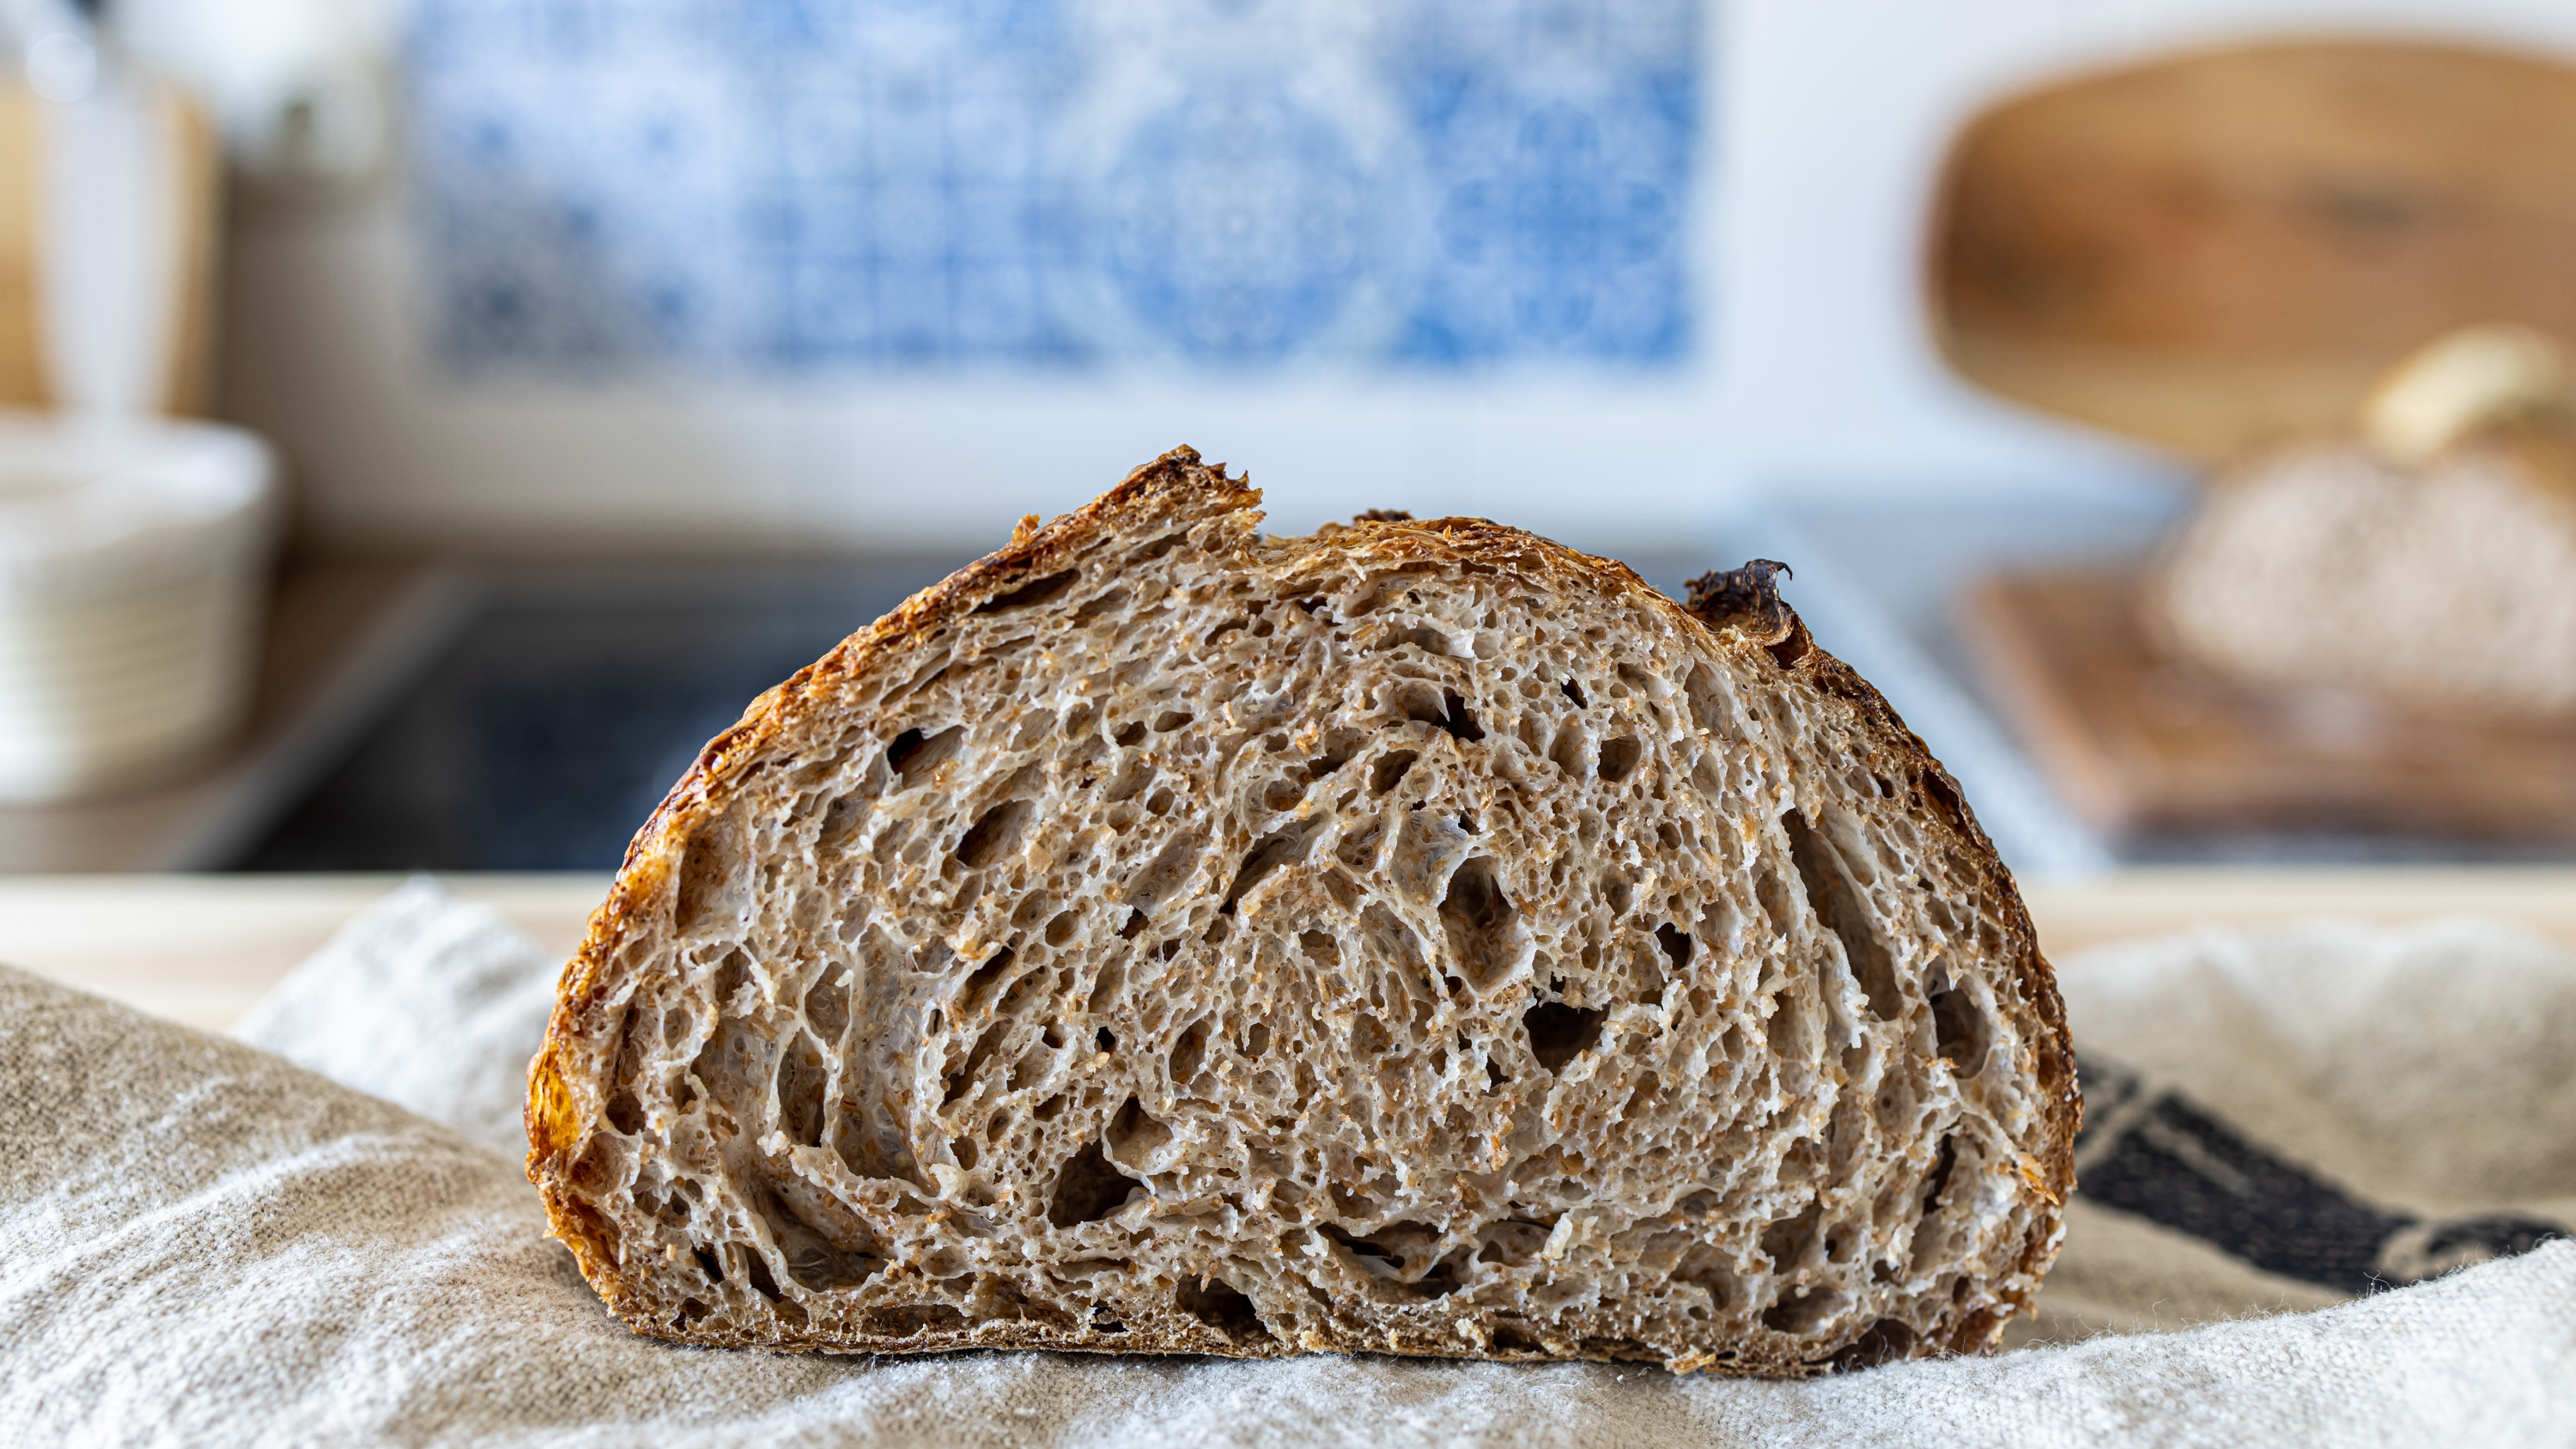
\includegraphics[width=\textwidth]{whole-wheat-crumb}
  \caption{A whole-wheat sourdough bread}
  \label{whole-wheat-crumb}
\end{figure}


By understanding the two key enzymes \textit{amylase} and \textit{protease}, you
will be better equipped to make bread to your liking. Do you prefer a softer
or stiffer crumb? Do you desire a lighter or darker crust? Do you wish to reduce
the amount of gluten in your final bread? These are all factors that you can
tweak just by adjusting the speed of your dough's fermentation.

\section{Yeast}

% Yeast is both the singular and plural form of the word unless you're
% specifically referencing a plural number of varieties or types, in which case
% "yeasts" would be correct.
Yeast are single celled microorganisms that belong to the fungi kingdom, and
spores that are hundreds of millions of years old have been identified by
scientists. There are a wide variety of species: So far, about 1,500 have been
identified. Unlike other members of the fungi kingdom such as mold, yeast do
not create a mycelium network \cite{molecular+mechanisms+yeast}.

\begin{figure}[!htb]
  \centering
  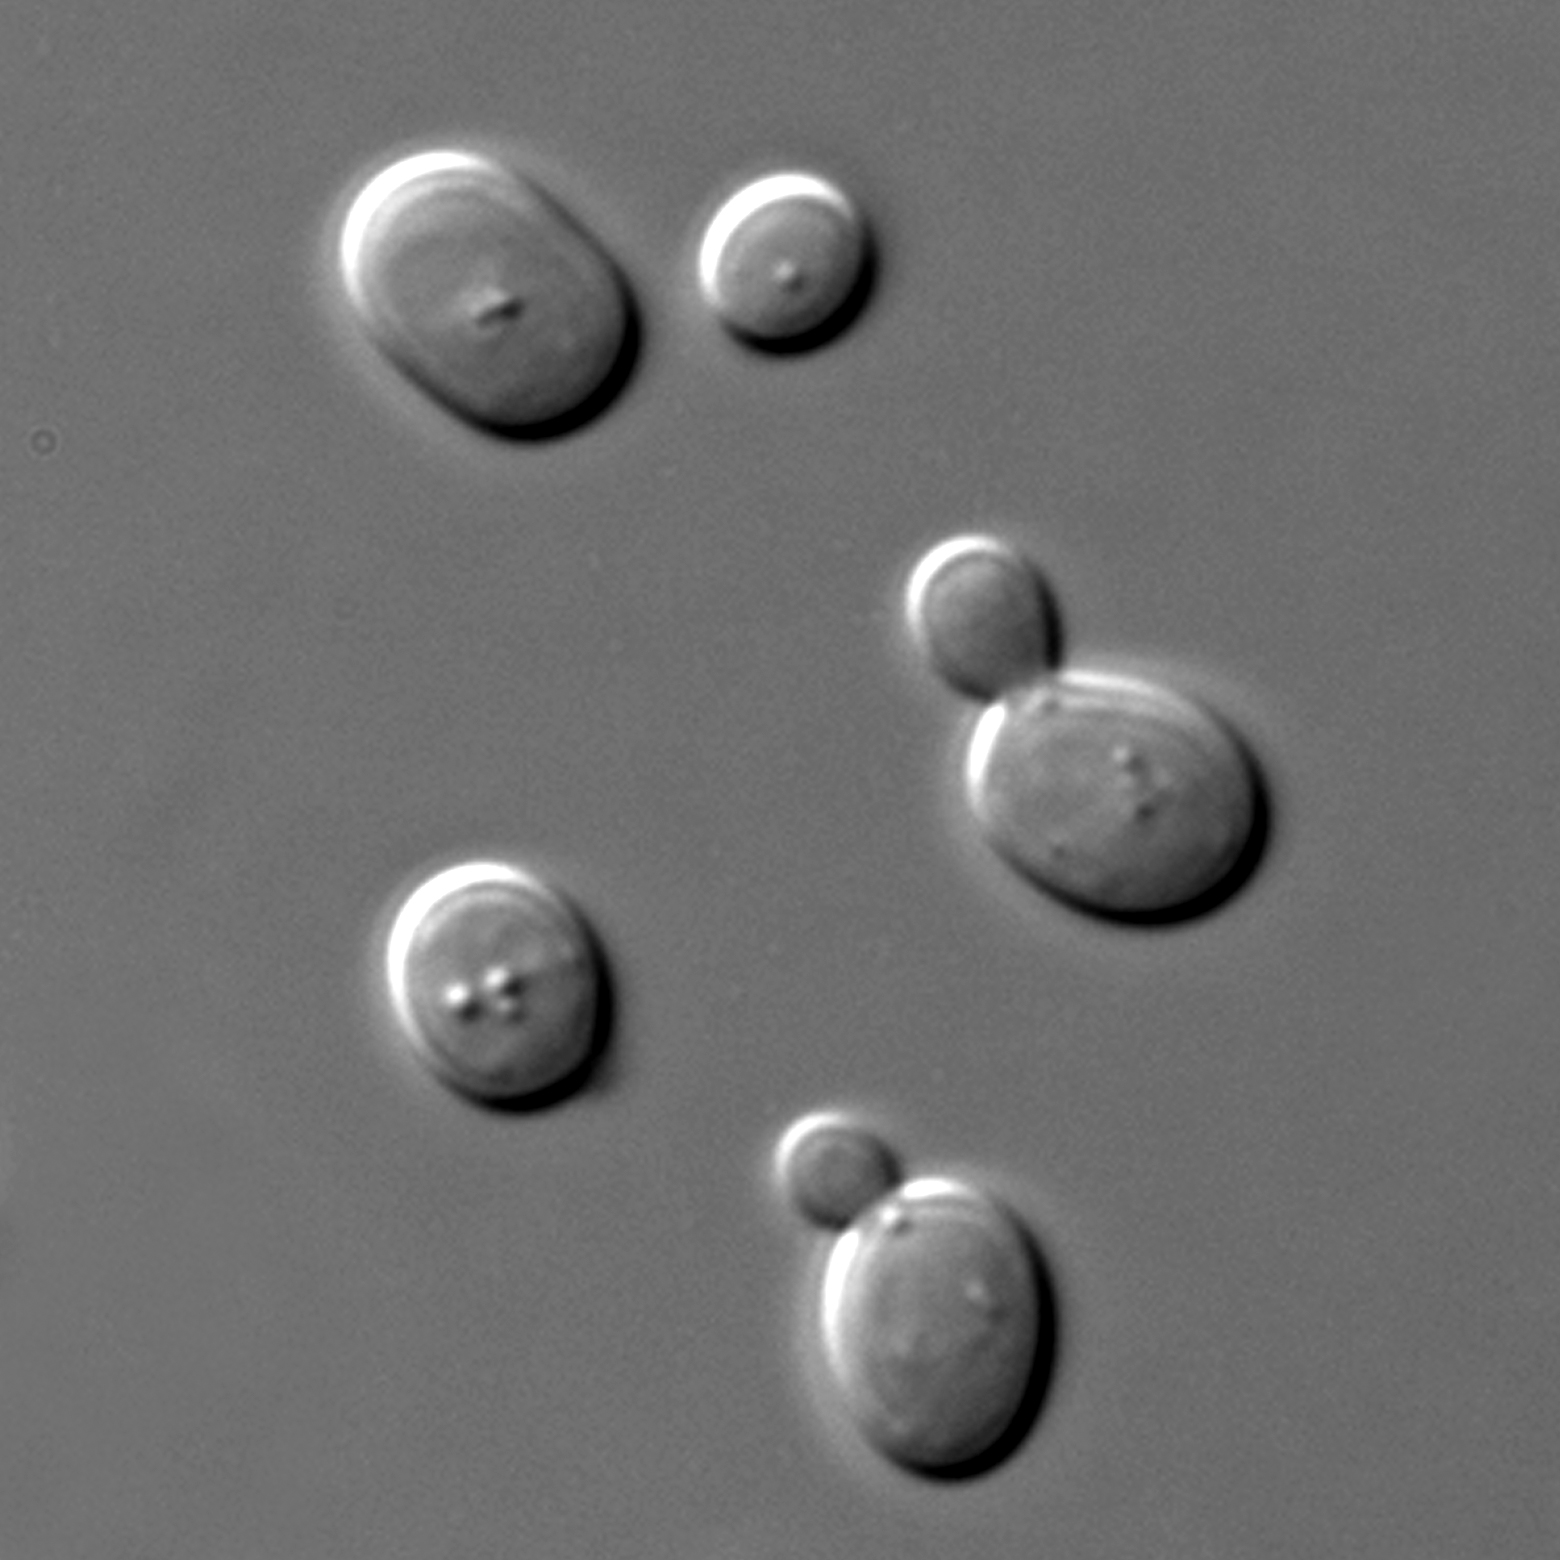
\includegraphics[width=1.0\textwidth]{saccharomyces-cerevisiae-microscope}
  \caption{Saccharomyces cerevisiae: Brewer's yeast under the microscope}
  \label{saccharomyces-cerevisiae-microscope}
\end{figure}

Yeast are saprotrophic fungi. This means that they do not produce their own
food, but instead rely on external sources that they can decompose and break
down into compounds that are more easily metabolized.

Yeast breaks down carbohydrates into carbon dioxide and alcohol in what we now
refer to as the fermentation process. This process has been known for thousands
of years and has been used since ancient times for the making of bread as well
as alcoholic beverages.

Yeast can grow and multiply under both aerobic and anaerobic conditions. When oxygen
is present the yeast almost completely produces
carbon dioxide and water. When no oxygen is present
the yeast starts switches its metabolism. The
yeast starts to produce alcoholic compounds \cite{effects+oxygen+yeast+growth}.
The temperatures at which the yeast grows vary. Some
yeasts such as {\it Leucosporidium frigidum} grows
best at temperatures between -2°C up to 20°C. Other
yeast grows better at higher temperatures. The warmer
it is the faster the yeast's metabolism works. The yeast
that you cultivate in your sourdough starter works best
at the temperatures where the grain was grown and at
the point when it was harvested. So if you are from a 
cooler place and cultivate a sourdough starter from
a nordic rye variety, then chances are your yeast
prefers this colder environment. As an example
beer makers discovered that a beneficial yeast lives
in the cold caves around the city of Pilsen, Czech Republic.
This yeast has produced excellent tasting beers at
lower temperatures. Varieties of these strains
are now used to make popular lager beers.

Yeasts in general are very common in the environment.
They can be found on cereal grains, fruits, other plants
in the soil and also in your gut. Very little is known
about the ecology of why yeasts we use for baking
are cultivating the leaves of the plants. The plants
are protected via the cell walls and hardly any
fungi and other bacteria can penetrate. Some fungi and
bacteria are producing enzymes that are able
to break down the cell walls and infect the plant.
There are fungi and bacteria that live within the plant
without causing any distress. These are known as {\it endophytes}.
They are not damaging the plant per se. In fact they are
living in a symbiotic relationship with the host. They
help the plant to protect itself from additional pathogens
that might enter through the leaves of the plant. They
help with water stress, heat stress and nutrient availability. 
In exchange for the service they receive carbon for energy
from the plant host. They are not always strictly mutualistic though.
Sometimes under stress conditions they can become pathogens
on their own \cite{endophytes+in+plants} and decay begin
decaying the plant.

The yeasts we use for baking are
living as as epiphytes on the plant. Compared to
the previously mentioned endophytes they are not
breaching the walls of the cells. Most of them
receive nutrients from rain water, the air or other animals.
These sources also include honeydew produced
by aphids. Pollen that lands on the leaf's surface
is an additional source of food. Interestingly
though when you remove that external food source,
you still find a large variety of epiphytic fungi
and bacteria on the plant's surface. The food
for them is coming directly from the plant it seems.
Some research has shown that the plants are
on purpose releasing some compounds such as sugars,
organic acids, amino acids, some methanol and various
salts via the surface. These nutrients would
then attract the epiphytes to live on the surface.
The plants benefit from enhanced protection against
mold and other pathogens. It is in the best interest
of the epiphytes to keep the plants alive
as long as possible \cite{leaf+surface+sugars+epiphytes}.
More and more research is conducted on using yeasts
as a biocontrol agents to protect plants. These bio-agents
would be food-safe as yeasts are generally considered save.
The yeasts would start to grow on the leaves on the plant
and essentially shield the plants from other molds. This
could be a game changer for wineyeards suffering from mildew.
This could also be helpful to shield the plant against the
psychoactive ergot fungus. The ergot fungus likes to grow
in more humid colder environments and poses a huge
problem to rye farmers. The fungus parasites the plant
and infects it. Consumption of ergot is not recommended
as it is highly toxic to the liver. That's why lawmakers
have recently reduced the amount of allowed ergot contamination
in rye flour. Another interesting experiment from Italian scientists
visualized how important yeasts could be when protecting
plants. They added tiny incisions into some of the grapes.
They would then infect some of the damaged surfaces with
mold. The other wounds they infected with some of the 150
different wild yeast strains isolated from the leaves plus
the mold. When mixing the mold with the yeast the grape
sustained no significant damage \cite{yeasts+biocontrol+agent}.
In another experiment however scientists have shown
how the brewer's yeast became an aggressive pathogen to wine plants.
Initially the yeast lived in symbiosis with the plant. After the grapevine
sustained damages the yeast became opportunistic and started to
attack the plant event producing hyphae to deeply
penetrate the plants tissue.

\section{Bacteria}

\chapter{Making a sourdough starter}
\chapter{Making a sourdough starter}%
\label{chapter:sourdough-starter}
\begin{quoting}

\begin{figure}[!htb]
  \centering
  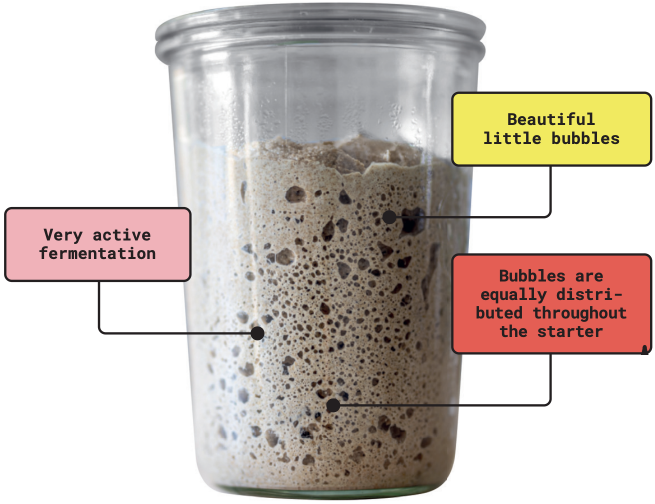
\includegraphics[width=\textwidth]{sourdough-starter-activity-indicators}
  \caption[Very active sourdough]{A very active sourdough starter shown by the
      bubbles in the dough.}%
  \label{fig:sourdough-starter}
\end{figure}

In this chapter you will learn how to make your
own sourdough starter, but before doing so you will
quickly learn about baker's math. Don't worry,
it's a very simple way how to write a recipe which
is cleaner and more scalable. Once you get the hang
of it you will want to write every recipe this way.
You will learn to understand the signs indicating
your starter's readiness, as well as
how to prepare your starter for long-term storage.
\end{quoting}

\iffalse

\section{Baker's math}%
\label{section:bakers-math}

In a large bakery, a determining factor is how
much flour you have at hand. Based on the amount
of flour you have, you can calculate how many
loaves or buns you can make. To make it easy
for bakers, the quantity of each ingredient
is calculated as a percentage based on how much flour you have.
Let me demonstrate this with a small example from
a pizzeria. In the morning you check and you realize you
have around \qty{1}{\kg} of flour.
Your default recipe calls for around \qty{600}{\gram} of water.
That would be a typical pizza dough, not too dry but
also not too wet. Then you would be using around \qty{20}{\gram}
of salt and around \qty{100}{\gram} of sourdough starter\footnote{This is my go to
pizza dough recipe. In Napoli modern pizzerias would use fresh or dry yeast.
However traditionally pizza has always been made with sourdough.}.
The next day you suddenly have \qty{1.4}{\kg} of flour
at hand and thus can make more pizza dough. What do you do?
Do you multiply all the ingredients by \num{1.4}? Yes you could,
but there is an easier way. This is where baker's math
comes in handy. Let's look at the default recipe with baker's
math and then adjust it for the \qty{1.4}{\kg} flour quantity.

\begin{table}[!htb]
\centering
  \begin{tabular}{@{}r@{g }lrr@{ = }r@{}}
\toprule
\multicolumn{2}{c}{\thead{Ingredient}}& \thead{Percentage} & \multicolumn{2}{c}{\thead{Calculation}} \\ \midrule
1000& flour             &100\%        & 1000g of 1000g & 100\% \\ 
 600& water             & 60\%        & 600g of 1000g  &  60\% \\ 
 100& sourdough starter & 10\%        & 100g of 1000g  &  10\% \\ 
  20& salt              &  2\%         & 20g of 1000g  &   2\% \\ \bottomrule
\end{tabular}

  \caption[Baker's math example]{An example table demonstrating how to
      properly calculate using baker's math}
\end{table}

Note how each of the ingredients is calculated as a percentage
based on the flour. The \qty{100}{\percent} is the baseline and represents the absolute
amount of flour that you have at hand. In this case that's
\qty{1000}{\gram}~(\qty{1}{\kg}).

Now let's go back to our example and adjust the flour, as we have
more flour available the next day. As mentioned the next day
we have \qty{1.4}{\kg} at hand (\qty{1400}{\gram}).

\begin{table}[!htb]
    \centering
        \begin{tabular}{@{}lrr@{ = }l@{}}
\toprule
\thead{Ingredient} & \thead{Baker's math} & \multicolumn{2}{c}{\thead{Calculated value}} \\ \midrule
Flour               & 100\%   & $1400 \times 1$ & 1400g         \\ \midrule
Water               & 60\%    & $1400 \times 0.6$ & 840g        \\ \midrule
Sourdough starter   & 10\%    & $1400 \times 0.1$ & 140g        \\ \midrule
Salt                & 2\%     & $1400 \times 0.02$ & 28g        \\ \bottomrule
\end{tabular}

        \caption[Another baker's math example]{An example recipe that uses
            \qty{1400}{\gram} as its baseline and is then calculated using
            baker's math.}
\end{table}

For each ingredient we calculate the percentage
based on the flour available (\qty{1400}{\gram}). So for the water
we calculate \qty{60}{\percent} based on \num{1400}. Open up your
calculator and type in \numproduct{1400 x 0.6} and you have
the exact value in grams that you should be using.
For the second day, that is \qty{840}{\gram}. Proceed to do the same
thing for all the other ingredients and you will know
your recipe.

Let's say you would want to use \qty{50}{\kg} of flour
the next day. What would you do? You would simply proceed
to calculate the percentages one more time. I~like this
way of writing recipes a lot. Imagine you wanted to make
some pasta. You would like to know how much sauce you should
be making. Now rather than making a recipe just for you, a
hungry family arrives. You are tasked with making pasta
for \num{20} people. How would you calculate the amount of sauce
you need? You go to the internet and check a recipe and then
are completely lost when trying to scale it up.
\fi

\section{The process of making a starter}

Making a sourdough starter is very easy, all you need
is a little bit of patience. It is in fact so easy that it can be summarized
in a simple flowchart~\ref{fig:sourdough-starter-process}.

\begin{flowchart}[!htb]
\centering
  \begin{tikzpicture}[node distance = 3.5cm, auto]
  \node [start] (init) {Mix \qty{50}{\gram} flour + \qty{50}{\gram} water, stir};
  \node [block, right of=init] (wait2) {Wait\\ \qty{24}{\hour}};
  \path [line] (init) -- (wait2);
  \node [block, below of=wait2, node distance=3.5cm] (feed) {\qty{10}{\gram} of previous day + \qty{50}{\gram} water + \qty{50}{\gram} flour, stir};
  \path [line] (wait2) -- (feed);
  \node [block, below of=feed] (discard) {Discard the rest};
  \path [line] (feed) -- (discard);
  \node [decision, right of=feed, node distance=3.5cm] (decide) {Is good?};
  \node [decision, above of=decide, node distance=3.5cm] (timeout) {Less than 10 feeds?};
  \node [fail, right of=timeout, node distance=3.5cm] (discard2) {Batch failed};
  \path [line] (timeout) -- node{no} (discard2);
  \path [line] (timeout) -- node{yes} (wait2);
  \path [line] (feed) -- (decide);
  \node [success, right of=decide, node distance=3.5cm] (use) {Ready to use};
  \path [line] (decide) -- node{no} (timeout);
  \path [line] (wait2) -- (feed);
  \path [line] (decide) -- node{yes} (use);

  \node [start, below of=discard, left of=discard] (start_n) { Start with Initial Mixture };
  \node [block, right of=start_n, node distance = 3.2cm] (wait_n) { Wait\\ \qty{24}{\hour} };
  \node [decision, right of=wait_n, node distance = 3.2cm] (readycheck_n) { Ready? };
  \node [block, below of=wait_n, node distance = 3cm] (feed_n) { Feed the Mixture };
  \node [decision, right of=feed_n, node distance = 3.2cm] (limitcheck_n) { Failed? };
  \node [fail, right of=limitcheck_n, node distance = 3.2cm] (abort_n) { Discard All, Start Over };
  \node [success, right of=readycheck_n, node distance = 3.2cm] (final_n) { Done };

  \draw [line] (start_n) -- (wait_n);
  \draw [line] (wait_n) -- (readycheck_n);
  \draw [line] (feed_n) -- (wait_n);
  \draw [line] (readycheck_n) -- node { No } (limitcheck_n);
  \draw [line] (limitcheck_n) -- node (feedok_n) { No } (feed_n) ;
  \draw [line] (limitcheck_n) -- node { Yes } (abort_n);
  \draw [line] (readycheck_n) -- node { Yes } (final_n);

  \node [below of=feedok_n, node distance=2cm, align=left] (details2) [shape=rectangle,draw,fill=white!90!black]{
    \fontsize{7}{9}\selectfont For the \emph{Initial Mixture}, mix \qty{50}{\gram} flour/\qty{50}{\gram} water.\\
    \fontsize{7}{9}\selectfont The Mixture is \emph{Ready} when it has
    \emph{grown}, has \emph{bubbles}, and \emph{smells}
    vinegary/yoghurty. \\

    \fontsize{7}{9}\selectfont The Mixture has \emph{Failed} when you
    have fed it too many (eg 10) times without success.\\

    \fontsize{7}{9}\selectfont To \emph{Feed the Mixture}, discard all but \qty{10}{\gram}, mix in \qty{50}{\gram} flour and \qty{50}{\gram} water.
  };
\end{tikzpicture}

  \caption[The full sourdough starter process]{The process of making a sourdough
      starter from scratch.}%
  \label{fig:sourdough-starter-process}
\end{flowchart}

The flour you should
use to bootstrap your starter is ideally a whole flour.
You could use whole-wheat, whole-rye, whole-spelt or
any other flour you have. In fact gluten free flours such
as rice or corn would also work. Don't worry, you can always
change the flour later. Use whatever whole flour you
already have at hand.

Your flour is contaminated with millions of microbes. As explained
before in the chapter about wild yeast and bacteria, these
microbes live on the surface of the plant. That's why
a whole flour works better because you have more natural
contamination from the microbes you are trying to cultivate
in your starter. More of them live on the hull compared to the
endophytes living in the grain.

Start by measuring approximately \qty{50}{\gram} of both flour and
water. The measurements don't have to be exact; you can use
less or more, or just eyeball the proportions. These
values are just shown as a reference.

Don't use chlorinated water when setting up your starter.
Ideally, you should use bottled water. In certain regions
like Germany, tap water is perfectly fine. Chlorine is added
to water as a disinfectant to kill microorganisms, you will
not be able to grow a starter with chlorinated water.

In this process, the hydration of your starter is \qty{100}{\percent}.
This means you're using equal amount of flour and
water. Stir everything together so that all the flour is
properly hydrated. This step activates the microbial spores
in your mixture, drawing them out of hibernation and
reviving them.
Finally, cover your mixture but make sure the covering is
not airtight. You still want some gas exchange to be possible.
I~like to use a glass and place another
inverted one on top.

Now an epic battle begins. In one study~\cite{yeasts+biocontrol+agent}
scientists have identified more than \num{150}~different yeast species living
on a single leaf of a plant.
All of the different yeasts and bacteria are trying to get
the upper hand in this battle. Other pathogens such as mold
are also being activated as we added water. Only the strongest
most adaptable microorganisms will survive.

\begin{figure}[!htb]
  \includegraphics[width=\textwidth]{sourdough-starter-microbial-war}
  \caption[Microbial warfare during sourdough early days]{A simple
      visualization of the microbial warfare that happens during the making of
      a sourdough starter. The wild spores on the plant and flour become
      activated the moment flour and water is mixed.  Only the most adapted
      flour-fermenting microbes will survive. Because of unwanted microbial
      fermentation it is advised to discard the feeding-leftovers of the first
      days. The surviving yeast and bacteria continuously try to outcompete
      each other for resources. New microbes have a hard time entering the
      starter and are eliminated.}%
  \label{fig:sourdough-starter-microbial-war}
\end{figure}

By adding water to the
flour the starches start to degrade. The seedling tries to
sprout but it no longer can. Essential for this process is the
amylase enzyme. The compact starch is broken down to more
digestible sugars to fuel plant growth. Glucose is what the
plant needs in order to grow. The microorganisms that survive
this frenzy are adapted to consuming glucose. 

Luckily for us
bakers, the yeast and bacteria know very well how to metabolize
glucose. This is what they have been fed in the wild by the plants.
By forming patches on the leaf and protecting the plant from
pathogens they received glucose in return for their services.
Each of the microbes tries to defeat the other by consuming the
food fastest, producing agents to inhibit food uptake by others or by producing
bactericides and/or fungicides. This early stage of the starter
is very interesting as more research could possibly reveal
new fungicides or antibiotics. 

Depending on where your flour
is from, the starting microbes of your starter might be different
than the ones from another starter. Some people have also reported
how the microbes from your hand or air can influence your starter's
microorganisms. This makes sense to a certain extent. Your
hand's microbes might be good at fermenting your sweat, but
probably not so good at metabolizing glucose. The contamination
of your hands or air might play a minor role in the initial epic
battle. But only the fittest microbes fitting the sourdough's
niche are going to survive. 

This means the microorganisms knowing
how to convert maltose or glucose will have the upper hand. Or the
microbes fermenting the waste of the other microbes. Ethanol created
by the yeast is metabolized by the bacteria in your sourdough. That's
why a sourdough has no alcohol. I~can confirm the role of aerial
contamination to a certain extent, when setting up a new sourdough
starter the whole process is quite quick for me. After a few
days my new starter seems to be quite alive already. This might
be due to previous contamination of flour fermenting microbes in
my kitchen.

Wait for around 24~hours and observe what happens to your starter.
You might see some early signs of fermentation already. Use your nose
to smell the dough. Look for bubbles in the dough. Your dough
might already have increased in size a little bit. Whatever
you see and notice is a sign of the first battle.

Some microbes
have already been outperformed. Others have won the first battle.
After around 24~hours most of the starch has been broken down
and your microbes are hungry for additional sugars. With a spoon
take around \qty{10}{\gram} from the previous day's mixture and place
it in a new container. Again --- you could also simply eye ball
all the quantities. It does not matter that much. Mix the \qty{10}{\gram}
from the previous day with another \qty{50}{\gram} of flour
and \qty{50}{\gram} of water. 

Note the ratio of 1:5. I~very often use
1~part of old culture with 5~parts of flour and 5~parts of water.
This is also very often the same ratio I~use when making a dough.
A dough is nothing else than a giant sourdough starter with slightly different
properties. I'd always be using around \qtyrange{100}{200}{\gram} of starter
for around \qty{1000}{\gram} of flour (baker's math: \qtyrange{10}{20}{\percent}).

Homogenize your new mixture again with a spoon. Then cover
the mix again with a glass or a lid. If you notice the top of
your mixture dries out a lot consider using another cover. The
dried-out parts will be composted by more adapted microbes such as
mold. In many user reports, I~saw mold being able to damage
the starter when the starter itself dried out a lot. 

You will
still have some mixture left from your first day. As this contains
possibly dangerous pathogens that have been activated make sure you discard
this mixture. A rule of thumb is to begin keeping the discard,
the moment you made your first successful bread. At that point
your discard is long-fermented flour that is an excellent addon
used to make crackers, pancakes or delicious hearty sandwich
bread\ldots I~also frequently dry it and use it as a rolling agent
for pizzas that I~am making.\footnote{Discarding starter when preparing
a new batch can be frustrating. With experience, bread-making
becomes more efficient, and excess discard is rarely produced. It is
possible to prepare just the right amount of starter
needed for bread dough. In fact, a fully depleted starter can even be revived
using a small portion of bread dough. Any leftover discard, rich in spores,
can also serve as a backup to create a new sourdough starter. Simply mix the
discard with a little flour and water, and it will spring back to life. That is a
great option if the starter was accidentally depleted. A practical approach
is to store all discard in a single jar in the fridge, adding new discard on
top as needed and using it whenever required.}

You should hopefully again see some bubbles, the starter increasing
in size and/or the starter changing its smell. Some people give
up after the second or third day, because the signs might no longer
be as dominant as they were on day one. The reason for this lies in only a few
select microbes starting to take over the whole sourdough starter. The most
adaptable ones are going to win, they are very small in quantity and will
grow in population with each subsequent feeding. Even if you see no signs
of activity directly, do not worry, there is activity in
your starter at a microscopic level.

24~hours later again we will repeat the same thing again until
we see that our sourdough starter is active. More on that in the
next section of this book.

\section{Determining starter readiness}

For some people the whole process of setting up a starter takes
only 4~days. For others it can take 7~days, for some even 20~days.
This depends on several factors including how good your wild microbes
are at fermenting flour. Generally speaking, with each feeding
your starter becomes more adapted to its environment. Your
starter will become better at fermenting flour. That's why
a very old and mature starter you receive from a friend might
be stronger than your own starter initially. Over time
your sourdough starter will catch up. Similarly, modern baking
yeast has been isolated like this from century old sourdough
starters.

\begin{flowchart}[!htb]
\centering
  \documentclass[tikz]{standalone}
\usepackage{tikz}
\usepackage{siunitx}
\DeclareSIUnit\degF{\text{°}F}

\begin{document}
\begin{tikzpicture}[node distance = 3cm, auto]
  \node [block] (init) {\footnotesize Make a starter};
  \node [block, right of=init, node distance=3cm] (feed) {\footnotesize Feed your starter};
  \path [line] (init) -- (feed);
  \node [block, right of=feed, node distance=3cm] (wait_12_after_feed) {\footnotesize Wait 12 hours};
  \path [line] (feed) -- (wait_12_after_feed);
  \node [block, right of=wait_12_after_feed, node distance=3cm] (ready_question) {\footnotesize Perform readiness check};
  \path [line] (wait_12_after_feed) -- (ready_question);
  \node [block, below of=feed, node distance=3cm] (wait_12) {\footnotesize Wait 12 hours};
  \path [line] (wait_12) -- (feed);
  \node [decision, right of=ready_question, node distance=3.5cm] (is_bubbly) {\footnotesize Bubbly? Size Increase?};
  \path [line] (ready_question) -- (is_bubbly);
  \path [line] (is_bubbly) -- node{no} (wait_12);
  \node [decision, below of=is_bubbly, node distance=4.0cm] (check_smell) {\footnotesize Vinegary, or yogurt smell?};
  \path [line] (is_bubbly) -- node{yes} (check_smell);
  \node [block, below of=init, node distance=6cm] (make_dough) {\footnotesize Make your dough};
  \path [line] (check_smell) -- node{yes} (make_dough);
  \path [line] (check_smell) -- node{no} (wait_12);
\end{tikzpicture}
\end{document}

  \caption[Determining sourdough starter readiness]{A flow chart showing you how to
      determine if your sourdough starter is ready to be used. Make sure to
      wait at least \qtyrange{6}{12}{\hour} after feeding your
      starter to check its readiness. To evaluate it, look at your starter's size
      increase, airy texture and take note of its smell.
      All three factors are important to properly evaluate your starter's activity level.
      An active starter is an important foundation for a successful dough fermentation}%
  \label{fig:sourdough-starter-readiness}
\end{flowchart}

The key sign to look at is bubbles that you see in your starter
jar. This is a sign that the yeast is metabolizing your
dough and creates \ch{CO2}. The \ch{CO2} is trapped in your dough
matrix and then visualized on the edges of the container.

Also note the size increase of your dough. The amount the dough increases
in size is irrelevant. Some bakers claim it doubles, triples or quadruples.
The amount of size increase depends on your microbes, but also on
the flour that you use to make the starter. Wheat flour contains
more gluten and will thus result in a larger size increase. At
the same time the microbes are probably not more active compared
to when living in rye sourdough. You could only argue that
wheat microbes might be better at breaking down gluten compared
to rye microbes. That's one of the reasons why I~decided to change
the flour of my sourdough starter quite often. I~had hoped to create
an all-around starter that can ferment all sorts of different
flour\footnote{Whether this is working, I~can't scientifically say.
Typically the microbes that have once taken place are very strong
and won't allow other microbes to enter. My starter has initially
been made with rye flour. So chances are that the majority of
my microorganisms are from a rye source.}.

Your nose is also
a great tool to determine starter readiness. Depending on
your starter's microbiome you should notice either the smell
of lactic acid or acetic acid. Lactic acid has dairy yogurty notes.
The acetic acid has very strong pungent vinegary notes. Some
describe the smell as glue or acetone. Combining the visual clues
of size increase and pockets plus the smell is the best way
to determine starter readiness.

In rare events your flour might be treated and prevent microbe growth.
This can happen if the flour is not organic and a lot of biochemical
agents have been used by the farmer. In that case simply try again
with different flour. Ten~days is a good period of time to wait before
trying again.

Another methodology used by some bakers is the so called \emph{float test}.
The idea is to take a piece of your sourdough starter and place it
on top of some water, if the dough is full with gas it will float
on top of the water. If it's not ready, it can't float and will
sink to the bottom. This test does not work with every flour,
rye flour for instance can't retain the gas as well as wheat flour
and thus in some cases will not float. That's why I~personally
don't use this test and can't recommend it.

Once you see your starter is ready I~would recommend giving it
one last feeding and then you are ready to make your dough in the
evening or the next day. For the instructions on how to make your
first dough please refer to the next chapters (\ref{chapter:wheat-sourdough}
and~\ref{chapter:non-wheat-sourdough}) in this book.

If your first bread failed, chances are your fermentation hasn't
worked as expected. In many cases the reason is your sourdough starter. Maybe
the balance of bacteria and yeast isn't optimal yet. In that case a good
solution is to keep feeding your starter once per day. With each feeding your
starter becomes better at fermenting flour. The microbes will adapt more and
more to the environment. Please also consider reading the stiff sourdough starter
chapter in this book. The stiff sourdough starter helps to boost the
yeast part of your sourdough and balance the fermentation.

\section{Maintenance}

\begin{flowchart}[!htb]
\centering
  \documentclass[tikz]{standalone}
\usepackage{tikz}
\usepackage{siunitx}
\DeclareSIUnit\degF{\text{°}F}

\begin{document}
\begin{tikzpicture}[node distance = 3cm, auto]
  \node [block] (init) {\footnotesize Make your bread dough};
  \node [decision, below of=init, node distance=3.5cm] (all_starter_used) {\footnotesize All starter used?};
  \path [line] (init) -- (all_starter_used);
  \node [block, right of=init, node distance=3cm] (use_dough) {\footnotesize Take 10g of your bread dough};
  \node [block, right of=all_starter_used, node distance=3cm] (use_starter) {\footnotesize Take all but not more than 10g of your starter};
  \path [line] (all_starter_used) -- node{yes} (use_dough);
  \path [line] (all_starter_used) -- node{no} (use_starter);
  \node [block, right of=use_dough, node distance=3cm] (feed_starter) {\footnotesize Feed using 1:5:5 ratio};
  \path [line] (use_dough) -- (feed_starter);
  \path [line] (use_starter) -- (feed_starter);
  \node [decision, right of=feed_starter, node distance=3cm] (bake_next_day_check) {\footnotesize Bake next day?};
  \path [line] (feed_starter) -- (bake_next_day_check);
  \node [block, right of=bake_next_day_check, node distance=3.5cm] (make_bread_dough) {\footnotesize Make bread dough again after 8-12 hours};
  \path [line] (bake_next_day_check) -- node{yes} (make_bread_dough);
  \node [decision, right of=use_starter, node distance=3cm] (bake_next_week_check) {\footnotesize Baking in next 2 weeks?};
  \node [block, right of=bake_next_week_check, node distance=3.5cm] (store_fridge) {\footnotesize Store starter in fridge at 4°C(40°F)};
  \path [line] (bake_next_week_check) -- node{yes} (store_fridge);
  \node [block, right of=store_fridge, node distance=3cm] (feed_after_fridge) {\footnotesize Feed again using 1:5:5 ration 8-12 hours before making dough};
  \path [line] (store_fridge) -- (feed_after_fridge);
  \path [line] (bake_next_day_check) -- node{no} (bake_next_week_check);
  \node [decision, below of=use_starter, node distance=3cm] (freezer_check) {\footnotesize Have a freezer?};
  \path [line] (bake_next_week_check) -- (store_fridge);
  \path [line] (bake_next_week_check) -- node{no} (freezer_check);
  \node [block, right of=freezer_check, node distance=3cm] (dry_starter) {\footnotesize Dry your starter};
  \node [block, below of=dry_starter, node distance=3cm] (freeze_starter) {\footnotesize Freeze your starter};
  \path [line] (freezer_check) -- node{no} (dry_starter);
  \path [line] (freezer_check) -- node{yes} (freeze_starter);
  \node [block, right of=dry_starter, node distance=3.5cm] (reactivate_freezer) {\footnotesize Reactivate starter for 3 days with daily 1:5:5 feedings};
  \path [line] (dry_starter) -- (reactivate_freezer);
  \path [line] (freeze_starter) -- (reactivate_freezer);
\end{tikzpicture}
\end{document}

  \caption[Sourdough starter maintenance flowchart]{A full flowchart showing
      you how to conduct proper sourdough starter maintenance. You can use a
      piece of your dough as the next starter. You can also use left-over
      starter and feed it again. Choose an option that works best for your own
      schedule. The chart assumes that you are using a starter at a
      \qty{100}{\percent} hydration level. Adjust the water content
      accordingly when you use a stiff starter.}%
  \label{fig:sourdough-maintenance-process}
\end{flowchart}

You have made your sourdough starter and your first bread. How do you perform
maintenance for your starter? There are countless different maintenance
methods out there. Some people go completely crazy about their starter and
perform daily feedings of the starter. The key to understanding how to properly
conduct maintenance is to understand what happens to your starter after you
used it to make a dough. Whatever starter you have left, or a tiny piece of
your bread dough can serve to make your next starter\footnote{I~very often use all my
starter to make a dough. So if the recipe calls for \qty{50}{\gram} of starter I~make
exactly \qty{50}{\gram} starter in advance. This means I~have no starter left. In that
case I~would proceed to take tiny bit of the dough at the end of the
fermentation period. This piece I~would use to regrow my starter again.}.

As explained earlier your starter is adapted
to fermenting flour. The microbes in your starter are very resilient. They
block external pathogens and other microbes. That is the reason why, when
buying a sourdough starter, you will preserve the original microbes. It is
likely that they are not going to change in your starter. They are outcompeting other
microbes when it comes to fermenting flour. Normally everything in nature
starts to decompose after a while. However, the microbes of your starter have
very strong defense mechanisms. In the end, your sourdough starter can be
compared to pickled food. Pickled food has been shown to stay good for a very
long period of time~\cite{pickled+foods+expiration}. The acidity of your sourdough starter is quite
toxic to other microbes. The yeast and bacteria though have adapted to living
in the high-acid environment. Compare this to your stomach, the acidity
neutralizes many possible pathogens. As long as your starter has sufficient
food available it will outcompete other microbes. When the starter runs out of
food the microbes will start to sporulate. They prepare for a period of no
food and will then reactivate the moment new food is present. The
spores are very resilient and can survive under extreme conditions.
Scientists have claimed they found 250 million-year-old spores that are still
active~\cite{old+spores}. While being spores
they are however more vulnerable to external pathogens such as mold.
Under ideal conditions though the spores can survive for a
long time.

But as long as they stay in the environment of your starter they live
in a very protected environment. Other fungi and bacteria have a hard time decomposing your left over starter mass.
I~have seen only very few cases where the starter actually died. It is almost impossible
to kill a starter.

What happens though is that the balance of yeast and
bacteria changes in your starter. The bacteria is more fitted to living
in an acidic environment. This is a problem when you make another dough.
You want to have the proper balance of fluffiness and sour notes.
When a starter has hibernated for a long period, chances are that
you do not have a desirable balance of microbes.
Furthermore, depending on the time your starter hibernated you might only have
sporulated microbes left. So a couple of feedings will help to get your
sourdough starter into the right shape again.

The following are a couple of scenarios that will help you to conduct proper
starter maintenance, depending on when you want to bake the next time.

\begin{description}
\item[I~would like to bake again the next day:]
Simply take whatever starter you have left and feed it again. If you depleted
all your starter you can cut a piece of your dough. The dough itself is
nothing different than a gigantic starter. I~recommend a 1:5:5 ratio like
mentioned before. So take 1 piece of starter, feed with 5 parts of flour and 5
parts of water. If it is very hot where you live, or if you want to make the
bread around 24~hours later after your last feeding, change the ratio. In that
case I~would go for a 1:10:10 ratio. Sometimes I~don't have enough starter.
Then I~even use a ratio of 1:50:50 or 1:100:100. Depending on how much new
flour you feed it takes longer for your starter to be ready again.

\item[I~would like to take a break and bake next week:]
Simply take your leftover starter and place it inside of your fridge. It will stay good
for a very long period. The only thing I~see happening is the surface
drying out in the fridge. So I~recommend drowning the starter in a little bit
of water. This extra layer of water provides good protection from the top
part drying out. As mold is aerobic it can not grow efficiently under
water~\cite{mold+anaerobic}. Before using the starter again simply either stir
the liquid into the dough or drain it. If you drain the liquid you can use it
to make a lacto-fermented hot sauce for instance.

The colder it is the longer you preserve a good balance of yeast and
bacteria. Generally, the warmer it is the faster the fermentation process is,
and the colder it is the slower the whole process becomes.
Below~\qty{4}{\degreeCelsius} the starter fermentation almost completely stops. The
fermentation speed at low temperatures depends on the
strains of wild yeast and bacteria
that you have cultivated.

\item[I~would like to take a several months break:]
Drying your starter might be the best option to preserve it in this case. As
you remove humidity and food your microbes will sporulate. As there is no
humidity the spores can resist other pathogens very well. A dried starter can
be good for years.

Simply take your starter and mix it with flour. Try to crumble the starter as
much as possible. Add more flour continuously until you notice that there is no
moisture left. Place the flour starter in a dry place in your house. Let it
dry out even more. If you have a dehydrator you can use this to speed up the
process. Set it to around~\qty{30}{\degreeCelsius} and dry the starter for 12--20~hours. The next
day your starter has dried out a bit. It is in a vulnerable state as there is still a bit
of humidity left. Add some more flour to speed up the drying process. Repeat
for another 2 days until you feel that there is no humidity left. This is
important or else it might start to grow mold. Once this is done simply store the
starter in an airtight container. Or you can proceed and freeze
the dried starter. Both options work perfectly fine. Your sporulated starter
is now waiting for your next feeding. If available you can add some silica
bags to the container to further absorb excess moisture.

Initially, it would take about three~days for my starter to become alive again
after drying and reactivating it. If I~do the same thing now my starter is
sometimes ready after a single feeding. It seems that the microbes adapt. The ones
that survive this shock become dominant subsequently.
\end{description}

So in conclusion the maintenance mode you choose depends on when you want to bake next.
The goal of each new feeding is to make sure your starter
has a desired balance of yeast and bacteria when making a dough. There is no need to provide your
starter with daily feedings, unless it is not mature yet. In that case, each
subsequent feeding will help to make your starter more adept at fermenting
flour.


\chapter{Sourdough starter types}
In this chapter of the book we will have a closer look
at different sourdough starter types and their respective
traits.

\begin{table}[htp!]
  \includegraphics{tables/table-starter-types.pdf}
  \caption{A comparison of different sourdough starter types and their
  respective properties. The only difference is the level of water (hydration)
  that is used when feeding the starter.}
  \label{tab:starter-types-comparison}
\end{table}

Depending on the flour you have at hand, the type of starter changes. With more
bacterial activity you have more gluten consumption of your microbes. So if
you want to bake a free standing loaf, you need a flour with more gluten. The
more gluten you have, the more of it can be broken down whilst still maintaining
dough integrity. If you live in a country where the climate to grow wheat
isn't ideal and you only have weaker flours, then a stiff sourdough starter
could be advised. The stiff sourdough starter will improve yeast activity and
reduce bacterial activity. If you are a chaser of a very sour bread and have a
very strong wheat flour then you can try to play with a liquid sourdough
starter. The key difference between all of the starters is how much water
is used in the starter. The regular starter has a 1:1 relationship of flour
to water. The liquid starter has a 5:1 water-to-flour ratio, and the stiff
starter has half the flour as water.

\begin{figure}[!htb]
  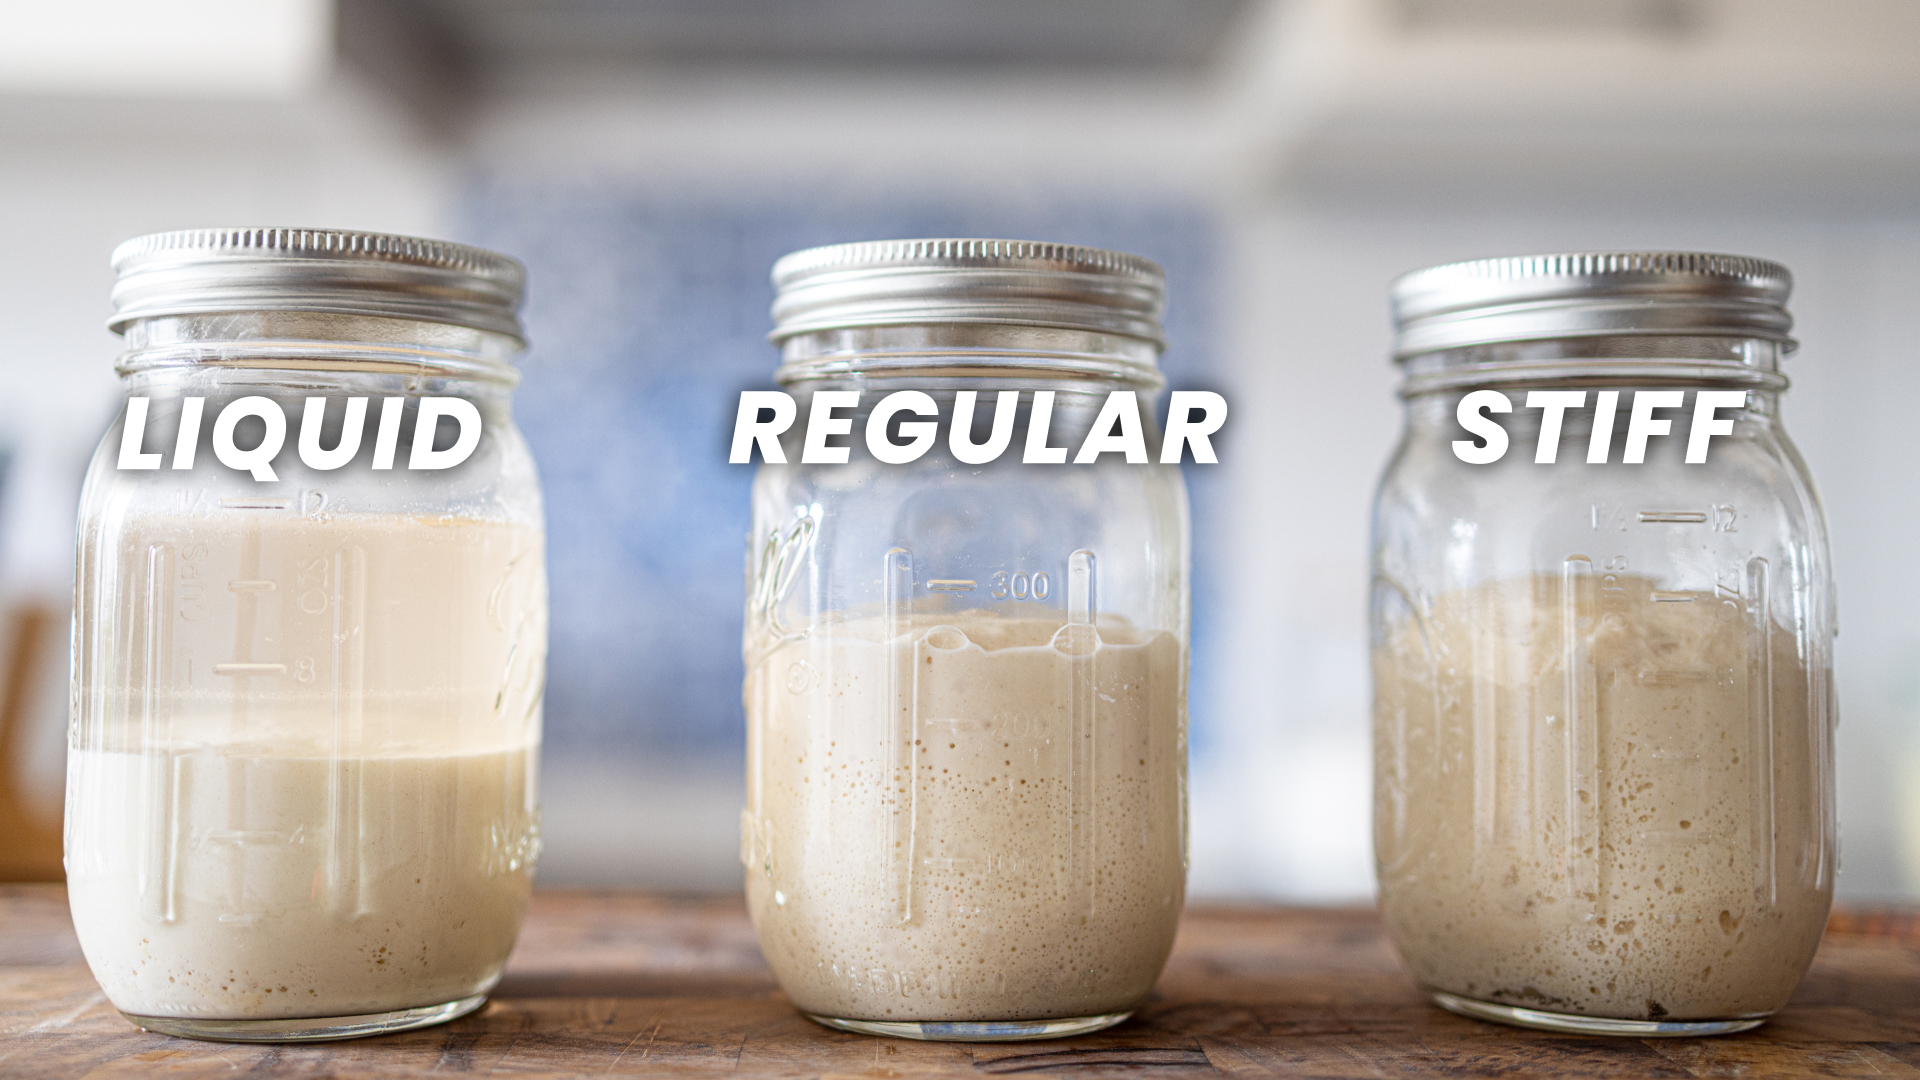
\includegraphics[width=\textwidth]{sourdough-starter-types}
  \caption{3 different starter types next to each other. Note how the liquid starter is submerged
  in water. It has a hydration of 500 percent or more.
  The regular starter has a hydration of around 100 percent, the stiff starter around 50 to 60 percent.}
  \label{fig:starter-types}
\end{figure}


You can change your starter type by just adjusting the feeding ratio of how
much flour and water you use. I frequently change my starter type from
regular to liquid and then back to a stiff starter. After changing the
environment of your microbes, apply feedings at the same ratio over a couple of
days so that they can adapt to the new environment. I typically see
changes after a single feeding, but I recommend 2 to 3 feedings, one feeding per
day, to see a stronger effect.

Your dough is generally just a big sourdough starter. So your starter is going
to adapt and regrow inside of your main dough. But you can influence the
properties that your starter carries over to your main dough. If you have more
bacterial fermentation, then your dough will also have slightly more bacterial
fermentation. If you have more yeast fermentation, then your main dough will
have slightly more yeast fermentation. This is important to know when you are
working with a more mature unfed starter. Let's say your starter had last been
fed 48 hours ago. Chances are that your bacteria is very active while the
yeast could be dormant. In such a case you can skip feeding your starter
before making another dough. Just use a very tiny amount of starter. For 1000 g
of flour I would take around 10 g of starter (1 percent in terms of baker's
math). If my starter is very young and had just been fed 6 to 8 hours ago I might
end up going up to 20 percent of starter. Remember that your dough is nothing
else other than a big starter. It will tremendously help you to figure out
your best next steps.

When using such a low inoculation rate (1 percent), you need to use stronger
flour when making wheat-based doughs. Your flour naturally breaks down due
to enzymatic activity. It might take 24 hours for the starter to re-grow
inside of your bread dough. At the same time, the enzymatic activity might
have caused your gluten to degrade significantly. While this is okay
when looking at your starter, your wheat-based dough will flatten
out during baking and no longer have the typical characteristics (fluffy crumb
structure). A stronger flour with more gluten is thus advised. It allows for
a longer fermentation before most gluten is broken down.

\section{Regular starter}

\begin{figure}[!htb]
  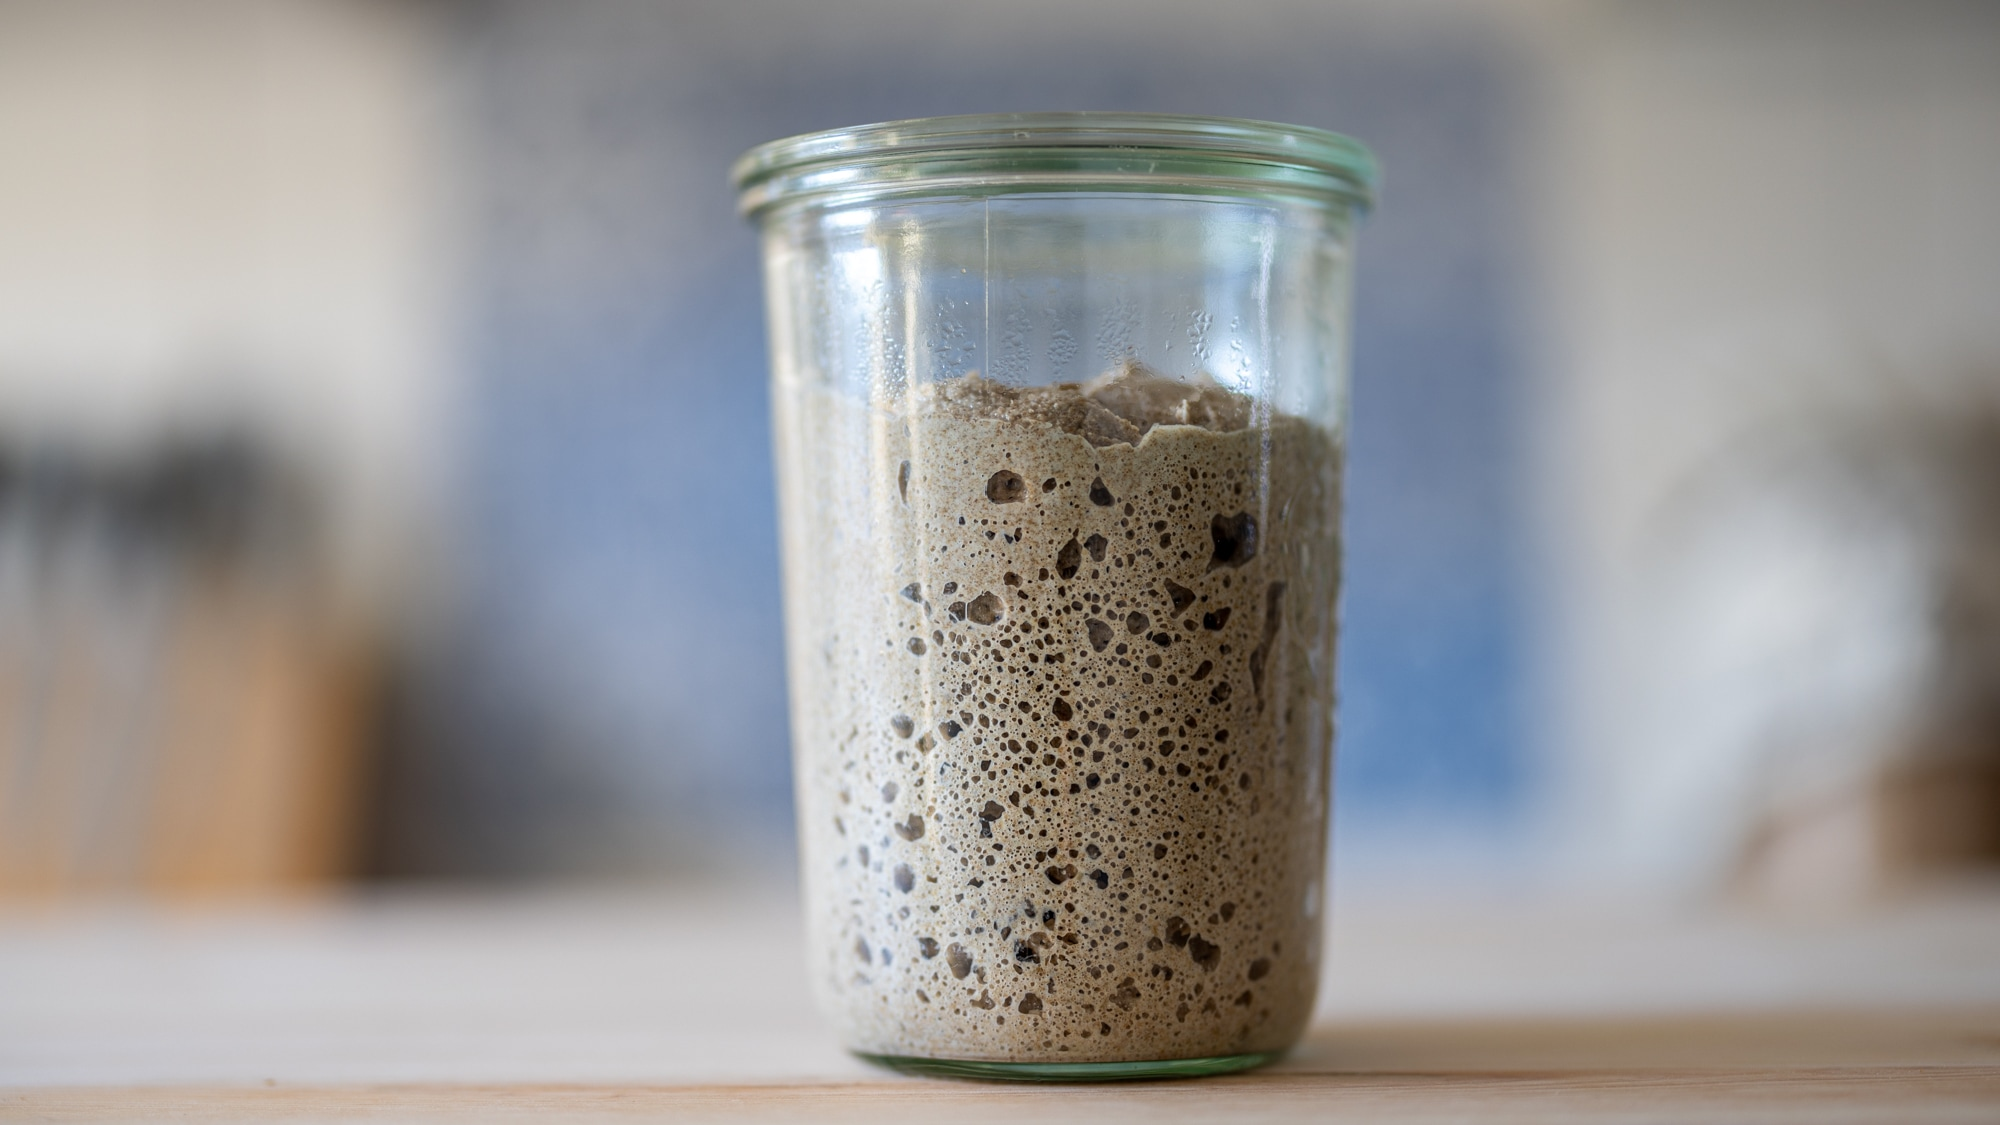
\includegraphics[width=\textwidth]{sourdough-starter.jpg}
  \caption{A regular sourdough starter at 100 percent hydration fed with rye flour}
  \label{fig:regular-sourdough-starter}
\end{figure}

The regular sourdough starter is made at a hydration of around 100 percent.
This means the starter has equal parts of flour and water. This is the most
common and must universal sourdough starter there is. The starter has a good
balance of yeast and bacteria. After a feeding, the volume increases and
increases. After it reaches a certain peak, it will start to collapse again.

The best way to judge whether the starter is ready is to look at signs such as
air pockets on the edges of your container. Also use the nose to evaluate the
smell of your starter. If you feel that the starter doesn't perform in a
desirable way, chances are that your yeast and bacteria ratios are off. In that
case frequent daily feedings using a 1:5:5 (starter:flour:water) ratio will
help.

A regular starter is a perfect choice to use when utilizing stronger wheat or spelt flours.
It also nicely works with rye, emmer or einkorn. If you only have a weak flour
at hand with less gluten, this starter might cause issues. As you tend to have
quite some bacterial activity, gluten is going to be broken down fast. When
using the starter, use around 1 to 20 percent starter based on the flour of your
dough.

Depending on the bacteria cultivated, a regular starter either has a lactic (dairy),
a vinegary (acetic) or mix of both flavor profiles. You can adjust your
starter's flavor by changing the type to a liquid starter.

\section{Liquid starter}
\label{section:liquid-starter}

\begin{figure}[!htb]
  \centering
  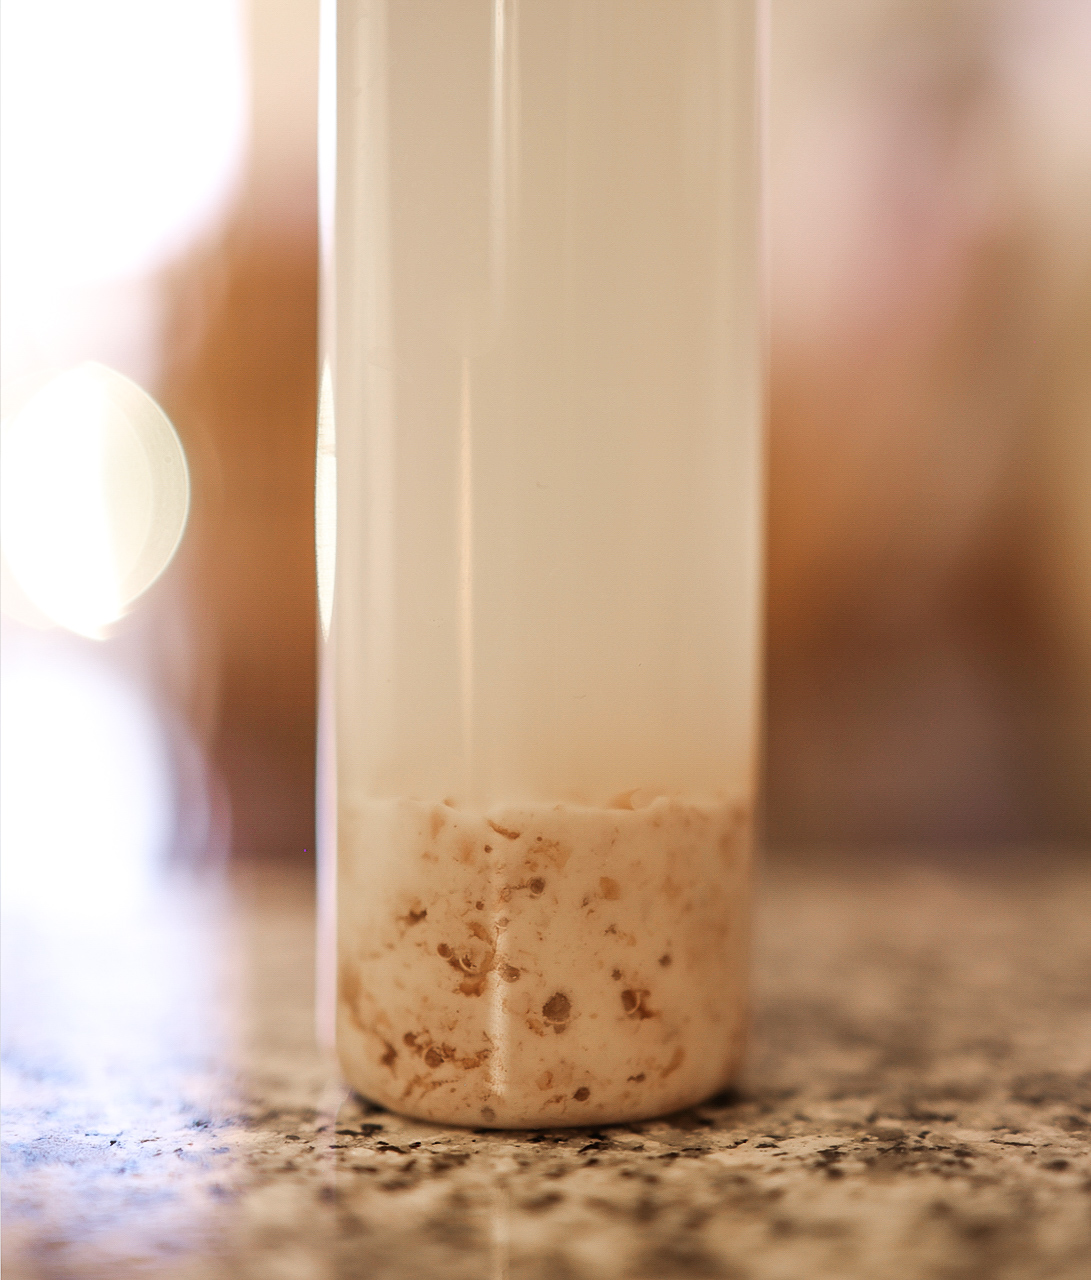
\includegraphics[width=0.5\textwidth]{sourdough-starter-liquid.jpg}
  \caption{A liquid sourdough starter features a high level of water. The high
  water amount boosts lactic acid producing bacteria. After a while the liquid
  and flour start to separate. Bubbles on the side of the flour
  indicate that the starter is ready to be used.}
  \label{fig:liquid-sourdough-starter}
\end{figure}


\begin{figure}[!htb]
  \includegraphics{figures/fig-liquid-starter-conversion.pdf}
  \caption{The process to convert your regular or stiff starter into a liquid starter. The whole
  process takes around 3 days. The longer you maintain your starter at the
  suggested hydration level, the more adapted your microorganisms become. It is recommended
  to keep a backup of your original starter as the liquid environment will select
  anaerobic microorganisms. This boosts bacteria that create lactic acid rather
  than acetic acid. The resulting acidity will be perceived as milder.}
  \label{fig:liquid-starter-conversion}
\end{figure}

The liquid starter is made at a hydration of around 500 percent. This means
the starter has much more water than flour. The additional layer of water on
top of the flour changes the microbiome of your starter.

By introducing this layer of water, less oxygen is available throughout the
course of fermentation. This means that your starter will no longer be
producing acetic acid. The heterofermentative lactic acid bacteria will thrive
in this environment. This is a neat little trick to change your starter's
flavor profile from vinegary to lactic. Your starter is going to develop
dairy creamy notes. Interestingly, when changing the hydration again, your starter
is going to maintain the liquid starter flavor profile, but then benefit again
from enhanced yeast activity. The liquid starter conversion is non reversible.
So ideally keep a backup of your stiff or regular starter.

To commence with the
conversion, simply take around 1 gram of your starter, mix with 5 g flour and
25 g water. Stir everything together properly. After a few minutes the flour is
going to start settling in at the bottom of your jar. Repeat this process over
a few days. Shake the starter gently to see if you can see tiny \ch{CO2} bubbles
moving in the liquid. This is a good sign that your starter is ready. Use your
nose to smell the starter. It should have a creamy dairy flavor note.

As you have more bacterial activity, this starter works best with a very strong
flour that can withstand a long fermentation period. Using this starter with a
weak wheat flour will not work. If you do not care about baking a freestanding loaf,
then you can easily use this starter together with a loaf pan.
This starter also works great when making a hearty pancake dough. To use it I
shake the starter container until I see all ingredients are homogenized. Then
I use around 5 percent of it in terms of baker's math. So for 1000 g of flour
that's around 50 grams of liquid starter. As it is very liquid you have to
include the 50 grams in your liquid calculation. I typically treat the starter
directly as liquid in the recipes. So if the recipe calls for 600 grams of water
and I use 50 grams of starter, then I would proceed and only use 550 grams of
water.

This type of starter is also an excellent mold combatant. As you are removing
oxygen from the equation, aerobic mold can not properly grow. If your starter
has a mold problem then the liquid conversion could be the remedy. Take a
piece of your starter where you suspect no mold growth. Apply the conversion
as mentioned before. The mold will likely sporulate as it runs out of food.
With each new feeding you are reducing the mold spores. The spores can no
longer reactivate as they can not do so in the anaerobic conditions.

The liquid on top of your starter is an excellent resource that you could use
to make sauces. If you feel you would like to add a little bit of acidity,
drain the liquid part on your starter and use it. I have used it numerous
times to make lacto-fermented hot sauces.

\section{Stiff starter}
\label{section:stiff-starter}

\begin{figure}[!htb]
  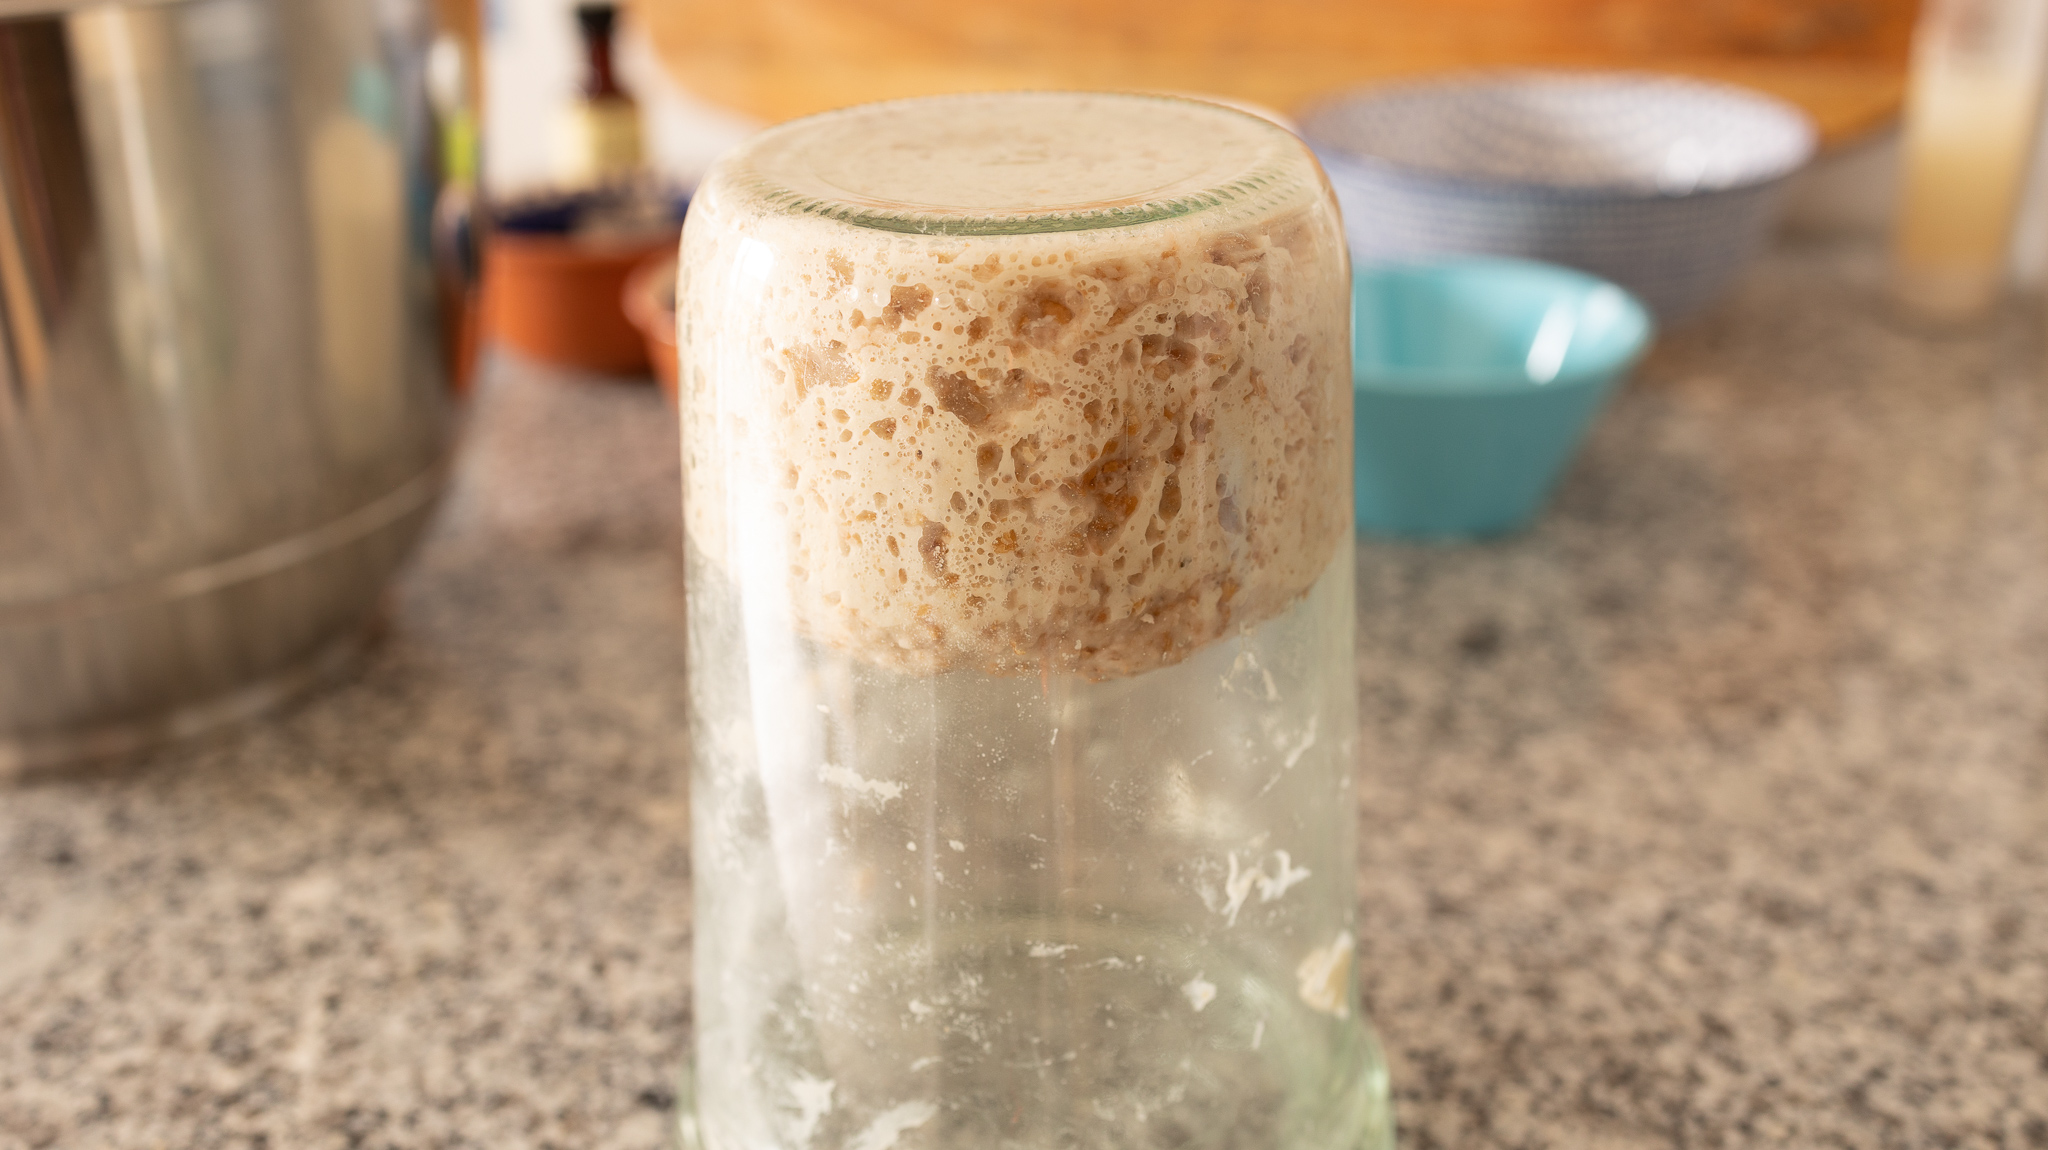
\includegraphics[width=\textwidth]{sourdough-starter-stiff.jpg}
  \caption{A stiff sourdough starter that I used to make a Stollen dough for Christmas. Note
  the bubbles on the edge of the container. The dough does not fall out of the jar.}
  \label{fig:stiff-sourdough-starter}
\end{figure}

The stiff starter is the driest of all the starters. It has a hydration of
around 50 to 60 percent. So for 100 grams of flour you are using around 50 to
60 grams of water.

\begin{figure}[!htb]
  \includegraphics{figures/fig-stiff-starter-conversion.pdf}
  \caption{The process to convert your regular starter into a stiff starter. The whole
  process takes around 3 days. The longer you maintain your starter at the
  suggested hydration level, the more adapted your microorganisms become. The
  stiff starter boosts the yeast activity of your sourdough starter.
  The guide uses a 50 percent hydration level for the starter. If the dough is too stiff
  consider increasing this to 60 percent.}
  \label{fig:stiff-starter-conversion}
\end{figure}

In the stiffer environment the yeast thrives more. This means you will have
more \ch{CO2} production and less acid production. In my tests this is a game
changer especially if you are using weaker gluten flours. The wheat flours in
my home country of Germany tend to be lower in gluten. For wheat to build gluten, warm conditions
are preferred (SOURCE NEEDED). When following recipes from other bakers, I
could never achieve similar results. When following timings my doughs would
simply collapse and become super sticky. Only when I started to buy more
expensive wheat flour did my results start to change. As not everyone can afford
these special baking flours and due to their limited availability, I stumbled upon the
stiff sourdough starter. I made several tests where I used the same amount of
starter and flour. I only changed the hydration between all the starters. I
would then proceed and place a balloon on top of each of the jars. The stiff
starter jar was clearly inflated the most. The regular starter
followed in second place. The liquid starter finished in third place with far less \ch{CO2}
production.

\begin{figure}[!htb]
  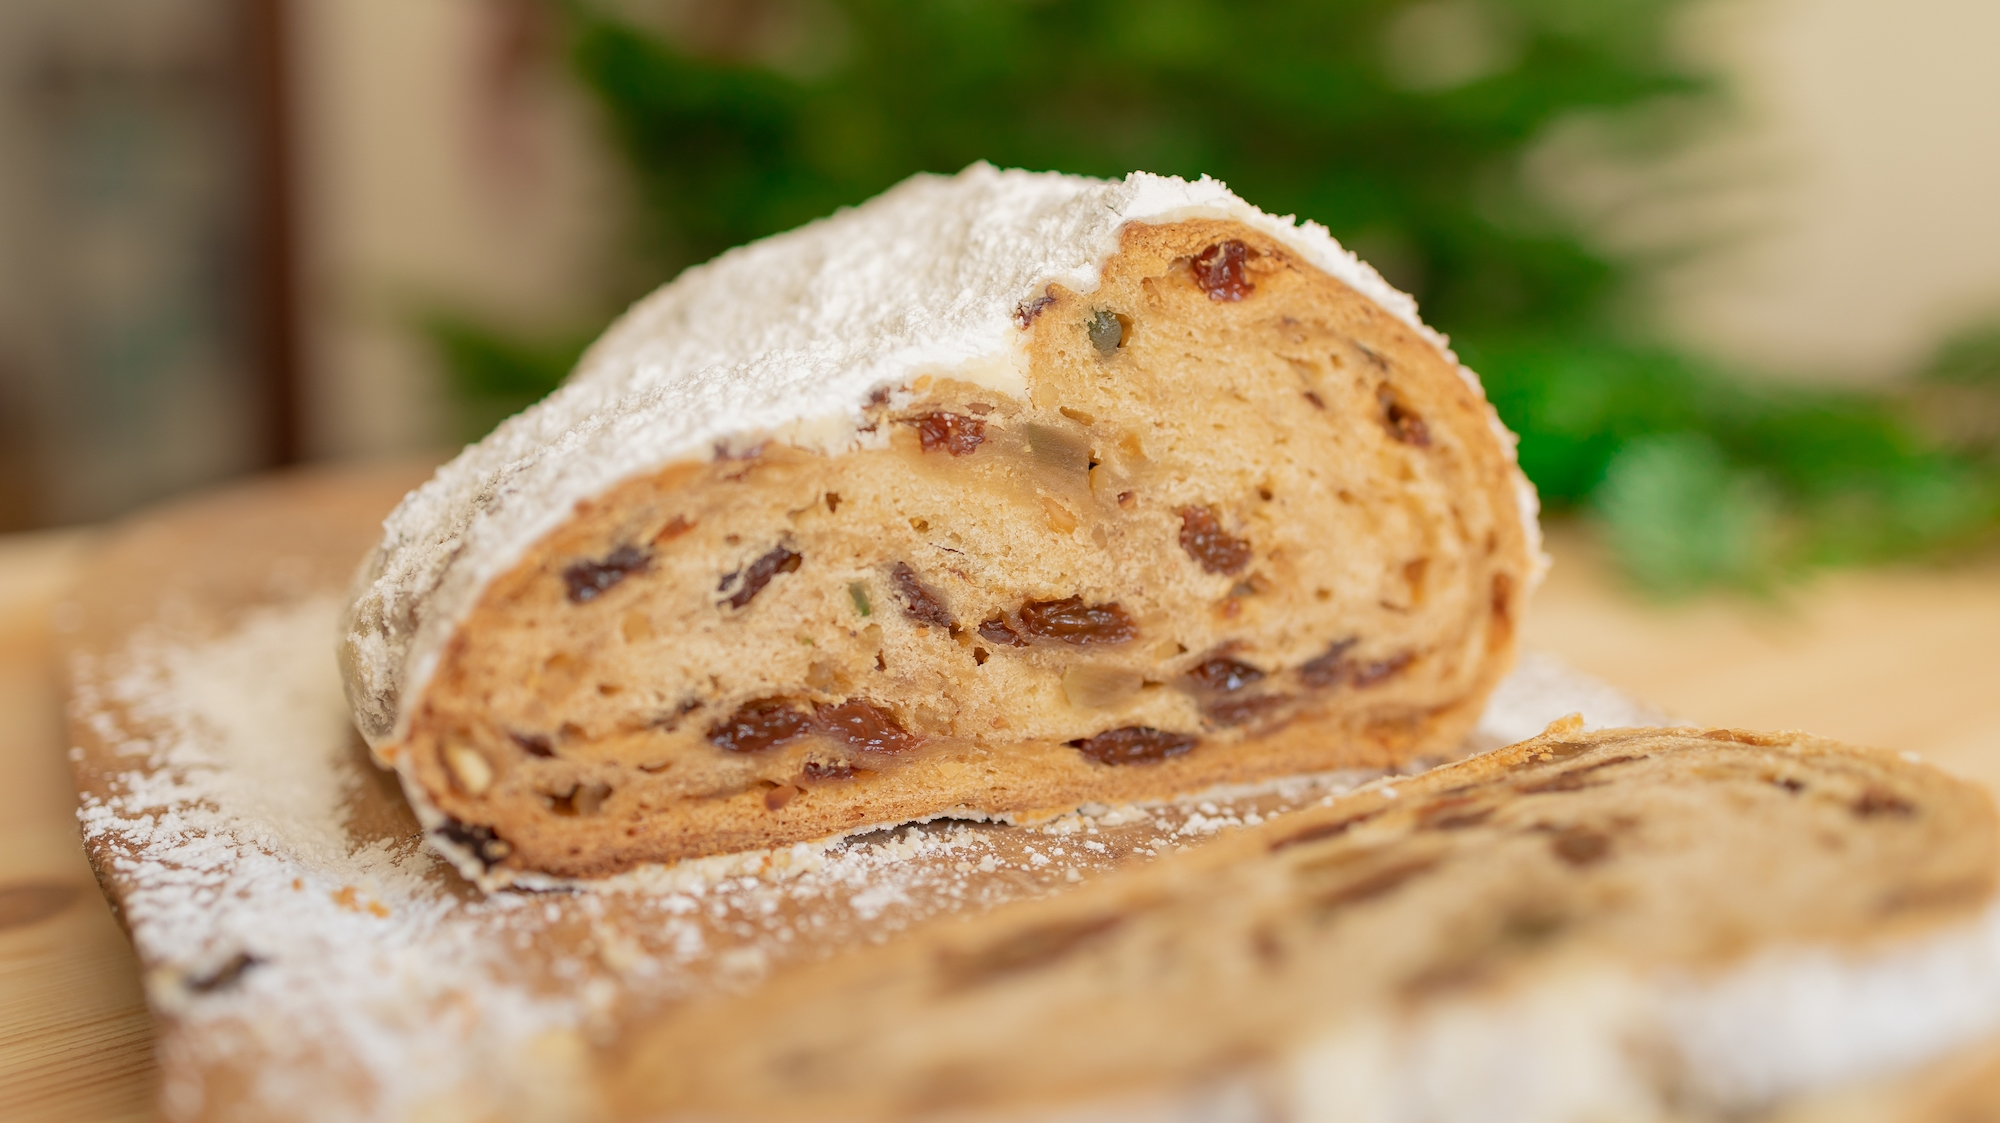
\includegraphics[width=\textwidth]{stollen}
  \caption{A German Christmas stollen made with a stiff starter instead of yeast}
  \label{fig:stollen}
\end{figure}

I then proceeded and bought a cheap low cake flour in my nearby supermarket.
This flour before had caused me massive headaches before. I made a sourdough bread
exactly how I would normally do. I had to reduce the hydration a bit as a low
gluten flour does not soak up as much water. Then I replaced the starter with
the stiff starter. The dough felt amazing and was suddenly able to withstand a
much longer fermentation period. The bread had great oven spring and tasted
very mild. I am still yet to find a proper explanation why the yeast part of
the dough is more active. Maybe it is not. It could also be that the bacteria
is inhibited by the lack of water.

When making the stiff sourdough starter, start by using around 50 percent
water. If you are using a whole wheat flour, or a strong flour consider going
up to 60 percent. All the ingredients should mix together very well. There
should be no crumbly flour left. This is a common mistake I have seen when
people tried to make the stiff starter. Yes it should be dry, but not to a
point where it is a brick of cement. If you have ever made a pasta dough, this
dough should exactly feel the same.

To evaluate whether your stiff starter is ready, look for a dome. Also look for
pockets of air on the sides of your container. Use your nose to smell the
starter. It should have a mild smell. It also tends to smell much more
alcoholic than the other starters.

When using a stiff starter, use around 1 to 20 percent depending on the ripeness of
your starter. In summer I typically use around 10 percent and in winter
around 20 percent. This way you can also control the fermentation speed.
Mixing the starter can be a little bit annoying as it hardly homogenizes with
the rest of the dough. In this case you can try to dissolve the starter in the
water you are about to use for your dough. This will make mixing a lot easier.


\section{Lievito madre or pasta madre}

The lievito madre, also known as pasta madre, belongs to the same category as
the stiff sourdough starter. After conducting hours of research, I could not
find a difference in pasta madre and lievito madre. Both terms seem to be
used interchangeably in literature.

In many recipes this starter is made directly
from dried or fresh fruits. You can also make a starter from leaves from your
garden. As described before, the wild yeast and bacteria consume the glucose
from the plants' leaves. All the options work. When making a starter directly
from dried fruits, you sometimes lack the bacterial part of the fermentation.
The acidity is very important in order to clean your starter from possible
pathogens. If you decide to make your starter from fruits, make sure it also
acidifies properly when making a dough. A tool such as a pH meter can be of
optimal help. Generally, the lower the pH, the higher the acidity. The acidity
should be below 4.2 to know that your starter produces sufficient acidity.

Some bakers cleanse the lievito madre in a bath of water. This is supposed to
remove excess acidity. In my own experiments I have not been able to confirm
this methodology. The acidity remains the same. The only reason this could
make sense is if you also tried to boost anaerobic microorganisms. However, then the
starter would need to remain in this environment for quite some time and not just
a few hours.

Baking with sourdough is simple. It's just flour and water. When seeing a recipe
from an experienced baker you wonder, Wait, that's it? There is nothing more
to it? I feel that this might be the reason why some bakers have such complicated
feeding procedures. They resort to several feedings per day at a certain given ratio.
This makes the baker feel a little more elitist. Of course over time as
more and more people follow this procedure, it becomes a self fulfilling prophecy.
The more experienced you become, the higher the chances are that a bogus starter
feeding guide will reward you with beautiful results. The reason however is
not in the starter routine. The reason is that you understand the fermentation better
and become better at reading the signs of your dough.

If I had to choose one starter type I would go for the stiff starter. In many cases
it will provide you with consistently great results with little effort.
In my experience you can make any yeast-based dough and just replace
the yeast directly with the stiff sourdough starter. You will be able
to achieve even better results with the stiff starter.

Lastly, no matter which starter type you choose, you can control how sour
you want your dough to be. The longer you push the fermentation, the more
acidity is going to be piled up. The only difference is that for a given
volume increase, the stiff starter will produce the least acidity. So for a
volume increase of 100 percent, the liquid starter has produced the most acidity,
followed by the regular starter and then the stiff starter. If you wait long
enough, the stiff starter will have produced the same amount of acidity as the
other starters. But before doing so it will have also produced a lot more \ch{CO2}. If
you like the sour flavor, you have to push your fermentation longer. This also
means you either need to bake in a loaf pan or have a very strong gluten flour
that is able to withstand long fermentation times.


\chapter{Flour types}
\begin{quoting}
In this chapter we will have a closer look at different flour types
and their respective categorization. We will also look at common
ways to distinguish different flours of the same type. This way you can more confidently
purchase the flour that you need.
\end{quoting}

The most basic flour type is a whole grain flour. In this case the whole seed has
been grounded to smaller pieces. Sometimes, depending on what you want to bake,
the hearty taste of the bran might not be desired. In this case you can use
whiter flours. With sieves, mills remove larger parts of the hull of the seed.
The seed already contains a pre-built germ from the plant waiting to be
activated. The whitest flour you can get is mostly just the starch part of the seed.
Depending on which layers are still present, names are used to describe the
type of flour.

\begin{table}[!htb]
    \begin{center}
        \begin{tabular}{@{}llrrr@{}}
\toprule
\textbf{USA}  & \textbf{UK}  & {\textbf{Germany}} & {\textbf{France}} & {\textbf{Italy}} \\ \midrule
Cake         & Soft flour  &  T405    &  T45   & 00 \\ 
All purpose  & Plain flour &  T550    &  T55   &  0 \\ 
             &             &  T812    &  T80   &  1 \\ 
             &             & T1050    & T110   &  2 \\ 
Whole        & Whole       & Vollkorn & T150   & Integrale \\ \bottomrule
\end{tabular}

        \caption[Labelling of wheat flour]{A comparison of how different types
            of wheat flour are labelled in different countries.}%
        \label{tab:flour-types-comparison}
    \end{center}
\end{table}

In Germany, the ash content is used to describe the flours. The lab will burn
\qty{100}{\gram} of flour in the oven. Then afterwards the remaining ash is extracted
and measured. Depending on the quantity the flour is categorized. If the flour
is of type 405 then \qty{405}{\mg} of ash have remained after burning the
flour. The more hull parts the flour has, the more minerals remain. So the
higher the number, the closer the flour is to whole flour. The numbers are
slightly different between each grain type. Generally though, the higher the
value, the heartier the taste is going to be.

\begin{figure}[htb!]
  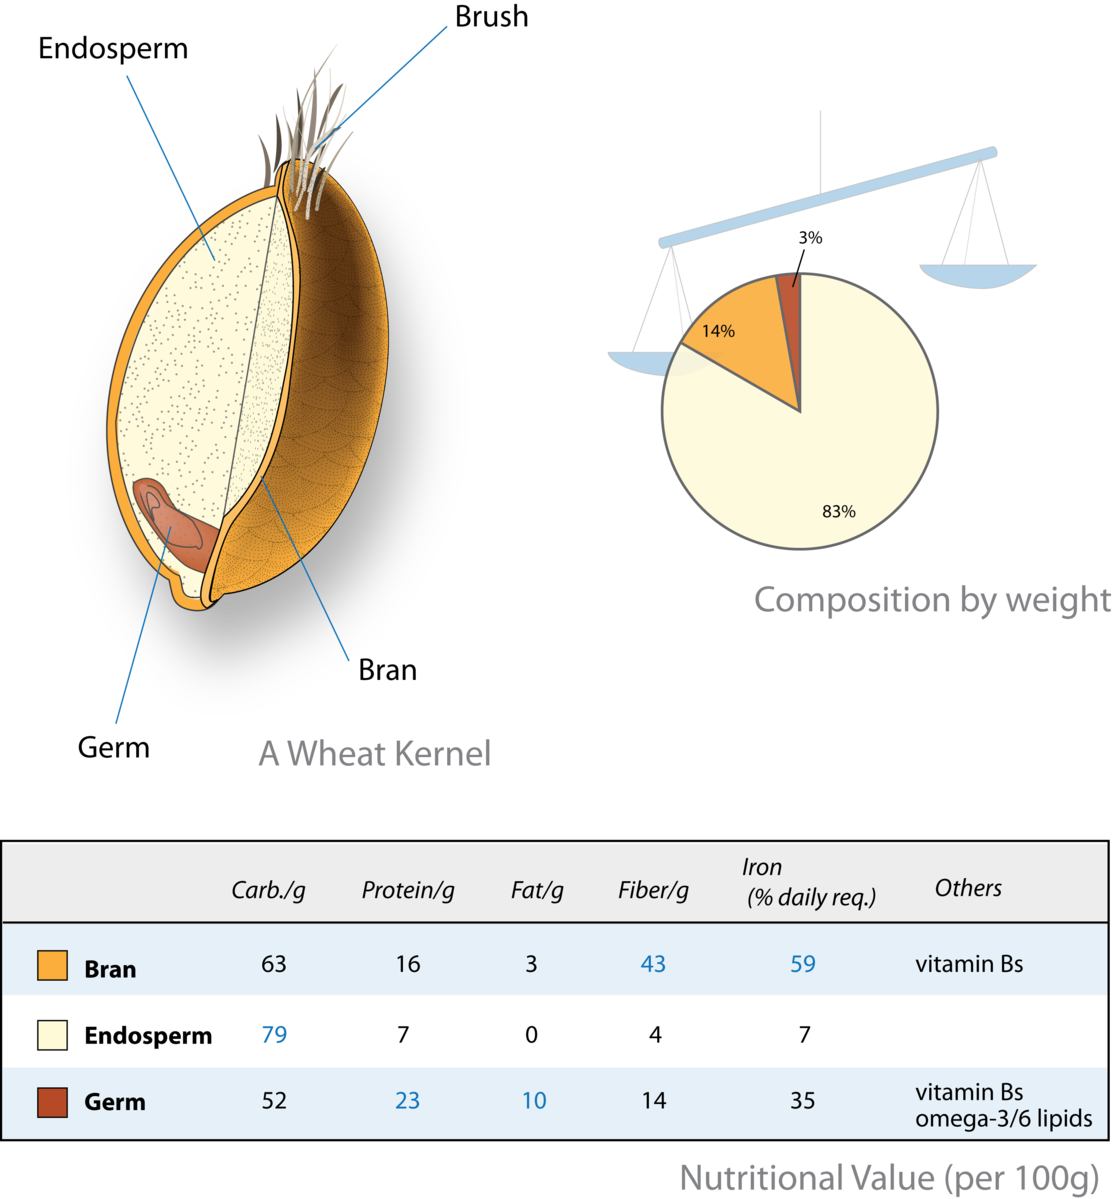
\includegraphics[width=\textwidth]{wheat-kernel-overview}
  \caption[Content of a wheat kernel]{An overview of a wheat kernel together
      with its content~\cite{wheat+kernel}.}%
  \label{fig:wheat-kernel-overview}
\end{figure}

If you compare different grain types, there are grains with high gluten, low gluten
and no gluten. Gluten is what enables bread to have its fluffy consistency.
Without gluten the baked goods wouldn't have the same properties. Managing
gluten makes the whole bread-making process more complex as more steps are involved.
A dough without gluten doesn't have to be kneaded. Kneading creates
the gluten bonds. The more you knead, the stronger they become. With low-gluten
and no-gluten flours, you only have to mix the ingredients together, making
sure you properly homogenize everything. During fermentation
the gluten degrades as the microorganisms metabolize it. When too much gluten
has been converted your dough will no longer have the wheat-like structure previously
described. For no/low gluten flour your main focus is managing acidity. You do not
want the final bread to be too sour. You do not have to worry about the gluten
degradation, removing a huge headache from the equation.

\begin{table}[!htb]
    \begin{center}
        \documentclass[tikz]{standalone}
\usepackage{tikz}
\usepackage{siunitx}
\DeclareSIUnit\degF{\text{°}F}

\begin{document}
\begin{tabular}{|l|l|l|l|l|}
\hline
\textbf{Grain type}              & \textbf{Homogenize} & \textbf{Knead} & \textbf{Stretch \& Fold} & \textbf{Shape} \\ \hline
\textbf{Wheat}                   & Yes                 & Yes            & Yes                      & Yes            \\ \hline
\textbf{\textgreater 70\% Wheat} & Yes                 & Yes            & Yes                      & Yes            \\ \hline
\textbf{Spelt}                   & Yes                 & Yes            & Yes                      & Yes            \\ \hline
\textbf{Rye}                     & Yes                 & No             & No                       & No             \\ \hline
\textbf{Emmer}                   & Yes                 & No             & No                       & No             \\ \hline
\textbf{Einkorn}                 & Yes                 & No             & No                       & No             \\ \hline
\textbf{Rice}                    & Yes                 & No             & No                       & No             \\ \hline
\textbf{Corn}                    & Yes                 & No             & No                       & No             \\ \hline
\end{tabular}
\end{document}

        \caption[Different types of grain]{An overview of different grain
          types and the steps involved in the respective bread making process.}
    \end{center}
\end{table}

As gluten has a special role, the rest of this chapter is dedicated to having a
closer look at different gluten flours and how to distinguish them. Spelt
also contains significant amounts of gluten, so the same characteristics hold
true.

Several recipes call for wheat bread flour. Bread flour can refer to different types
of flour. It could be a T405 or a T550 in Germany. This is very often
classified incorrectly. The terms \emph{strong} or \emph{bread} flour in this case
refer to the properties of the flour. A bread flour is considered to have a
higher amount of protein and thus gluten. This flour is excellent when you
want to make a sourdough bread as your dough allows for a longer leavening
period. As described earlier, the gluten is consumed by your microorganisms.
The more gluten you have, the longer your dough keeps its integrity. If you wanted
to make a cake, you might want to use a flour with less gluten. The gluten binding
properties might not be desirable since the final cake could have a chewy texture.

In conclusion, not every T405, T45 or T00 flour is the same. Depending on the properties
of the plant they come from, the flours will have different properties. For that reason
some countries like Germany have introduced additional scales to evaluate the quality of the
wheat. The category \textbf{A} refers to good quality wheat that can be blended
with poorer qualities to improve the flour. The category \textbf{B} refers to
average wheat that can be used to create different baked goods. Category \textbf{C}
is used for wheat that has poor baking qualities. This could happen, for instance,
if the wheat already started to sprout and thus lost some of its desirable
baking properties. This type of wheat is typically used in animal feed or
as fermentable biomass for generators. Category \textbf{E} refers to \emph{Elite} wheat. It's
the highest quality of wheat. This kind of wheat can only be harvested when the
wheat has grown under optimal conditions. You can compare this to a winery
that uses only the best grapes to make a reserve wine. Unfortunately, this is normally never printed
on the packaging of the flour that you buy. You can look out for the protein
value as a possible indicator. However, large mills blend flours together to
maintain quality throughout the years. Blended flour is also not listed on
the packaging. It might be that bakeries extract gluten from some flour and
then mix it in order to create better baking flours.

In Italy the so-called
\textbf{W-value} has been introduced to better show how the flour will behave.
A dough is made, and then the resistance of this dough to kneading is measured.
The more gluten a flour has, the more elastic the dough is, and the more it will
resist kneading. A higher W flour will have a higher gluten content and allow for a longer
fermentation period. But at the same time, it is also harder for the microbes to
inflate the dough as there is more balloon material. To make an excellent fermented
product out of a high W flour you will need to have a long fermentation period.
The long fermentation period also means that your microbes will enrich
your dough with more flavor.

\begin{table}[!htb]
    \begin{center}
        \begin{tabular}{@{}rcll@{}}
\toprule
\textbf{W-Value} & \textbf{Hydration (\%)} & \textbf{Uses} & \textbf{Fermentation time} \\ \midrule
0--150          & 50     & Cookies             & Very short    \\ 
150--250        & 50--60 & Cakes, Bread, Pizza & Short--Medium \\ 
250--350        & 60--70 & Bread, Pizza        & Long          \\ 
350+            & 70--90 & Bread, Pizza        & Very long     \\ \bottomrule
\end{tabular}

        \caption[Fermentation time versus W-value]{An overview of different
            levels of W-values and the respective hydrations and fermentation
            times.}%
        \label{tab:w-value}
    \end{center}
\end{table}

Generally, when aiming to
bake free standing sourdough bread, aim for a higher protein content. If the
gluten value is relatively low, your bread will collapse faster. Baking bread
is still possible, but it might be easier to use tools such as a loaf pan, or
to make skilled bread or flatbread.

An additional, rarely considered characteristic of good flour is the level of damage to the
starch molecules. This is a common problem when you are trying to mill your own wheat flours at
home. The chances are that your home mill is not able to achieve the same results
a larger mill can. The damaging of the starches is essential to improve the
properties of the dough. You will have better gelatinization and water
absorption with properly damaged starch~\cite{starch+damage+flour}. As more
starch is damaged, the surface area increases. This improves how water interacts with the flour.
This also provides a larger surface that your microbes can use to attack the molecules
and start the fermentation process.

I~am still
yet to find a good way of milling my own flour at home. Even after trying to
mill the flour 10 times with short breaks, I~was not able to achieve the same
properties as with commercially milled flour. The doughs I~would make felt
good, maybe a bit coarse. However, during baking the doughs would start to
de-gas quickly and turn into very flat breads. I~have had great success though when
utilizing home-milled flour together with a loaf pan or as a pan bread. If you
have found great ways to work with home-milled flour, please reach out. The potential
of using home-milled flours is huge. It would enable even distant communities
to grow their own wheat and be able to produce amazing freshly baked bread.


\chapter{Bread types}
\chapter{Bread types}%
\label{ch:bread-types}
\begin{quoting}
In this chapter you will learn about different bread types and their
advantages and disadvantages.  You can also find very simple recipes for
flatbread and pan loaf.  The former is probably the most accessible, least
effort type of bread you can make, while the latter is a little more involved.
Free standing bread has its own chapter, due to its increased complexity.
\end{quoting}

\section{Introduction}%
\label{sec:intro}

In this section we classify bread by its baking techniques. The appearance and
taste will of course be different, but you can get excellent bread with each
of them. Some breads will require investment and technique, as depicted in
Table~\ref{tab:bread-types-comparison}.  Flatbread is probably the most
accessible, least effort type of bread you can make. If you are a busy person
and/or don’t have an oven, this might be exactly the type of bread you should
consider.
\begin{table}[!htb]
    \centering
        \documentclass[tikz]{standalone}
\usepackage{tikz}
\usepackage{siunitx}
\DeclareSIUnit\degF{\text{°}F}

\begin{document}
\begin{tabular}{|l|l|l|l|}
\hline
                                 & \textbf{Flat bread} & \textbf{Loaf pan bread} & \textbf{Free standing bread} \\ \hline
\textbf{Cooking method}          & Fire, pan, barbecue & Oven                    & Oven                         \\ \hline
\textbf{Working time in minutes} & 3                   & 5                       & 60                           \\ \hline
\textbf{Flour types}             & All                 & All                     & Gluten flours                \\ \hline
\textbf{Difficulty}              & Very easy           & Easy                    & Difficult                    \\ \hline
\textbf{Cost}                    & Low                 & Medium                  & High                         \\ \hline
\end{tabular}
\end{document}

        \caption[Different bread types]{An overview of different bread types
            and their respective complexity.}%
        \label{tab:bread-types-comparison}
\end{table}

\section{Flatbread}%
\label{sec:flatbread}

Flatbread is probably the simplest sourdough bread to make.
To make a flatbread no oven is required; all you need is a stove.

\begin{figure}[!htb]
  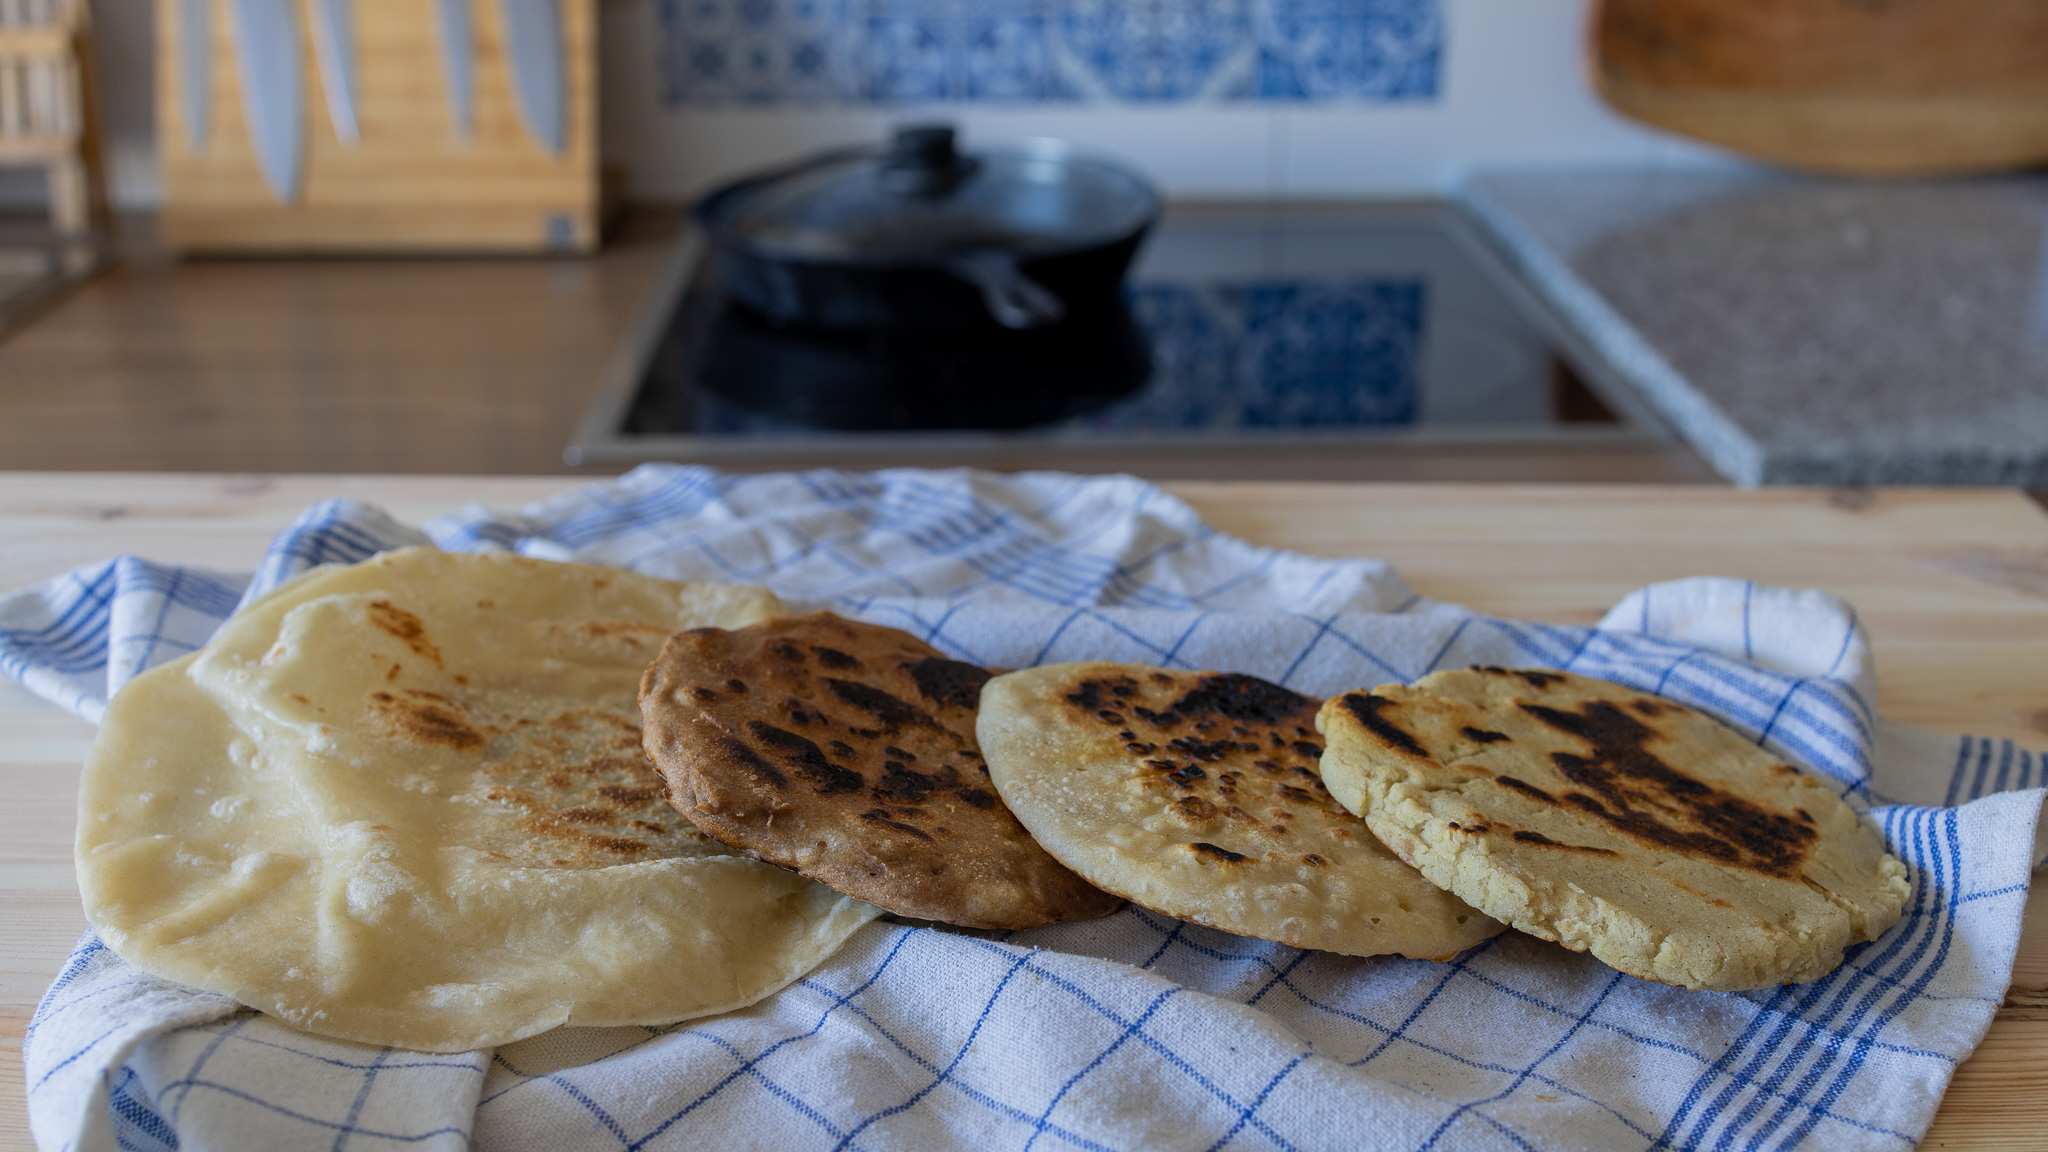
\includegraphics[width=\textwidth]{flat-breads-selection}
  \caption[Flatbread selection with different flours]{An assorted selection of
      different flatbreads made with sourdough. From left to right:
      Wheat~tortilla, rye, spelt and corn.}%
\end{figure}

This type of bread is super simple to make as you can skip
a lot of the technique that is normally required to make wheat doughs.
The flatbread can be made with all kinds of flours. You can even use
flour without gluten, such as corn or rice flour, to make the
dough. To make the flatbread a little more fluffy, you
can use a little bit of wheat flour. The developing gluten
will trap the gases. During baking, these gases will
inflate the dough.

Another trick to improve the texture of the flatbread is to
make a very wet dough. A lot of the water will evaporate
during the baking process and thus make the bread fluffier.
If your water content is very high, it will produce a
pancake-like consistency, as you can see in
Table~\ref{tab:flat-bread-ingredients}

\begin{table}[!htb]
    \centering
        %TODO: last line is not great
\begin{tabular}{@{}>{\bfseries} p{0.15\textwidth}rlrl@{}}
\toprule
      & \multicolumn{2}{c}{\thead{Flat breads}} & \multicolumn{2}{c}{\thead{Pancakes}} \\ \midrule
Flour             & 100g   &           & 100g   &           \\ 
Water             & 100g   & (100\%)   & 300g   & (300\%)   \\ 
Sourdough starter & 5--20g & (5--20\%) & 5--20g & (5--20\%) \\ 
Salt              & 2g     & (2\%)     & 2g     & (2\%)     \\ 
Bake when?        & \multicolumn{2}{c}{Dough increased by 50\% in size.}
                  & \multicolumn{2}{c}{Bubbles visible on surface.}\\
\bottomrule
\end{tabular}

        \caption[Flatbread recipe]{Flatbread or pancake recipe for 1 person.
            Multiply the ingredients to increase portion size.  Refer to the
            Section~\ref{sec:bakers-math}
            ``\nameref{sec:bakers-math}'' to learn how to understand and
            use the percentages properly.}%
            \label{tab:flat-bread-ingredients}
\end{table}

For a full recipe including the process of making such a flatbread,   refer to
Subsection~\ref{subsec:flat-bread-recipe}

\subsection{Flatbread framework}%
\label{subsec:flat-bread-framework}

As explained above, if you are just getting started, making a flatbread is the
easiest way to start making great bread at home. With just a
few steps, you can stop buying bread forever. This works with
any flour, including gluten-free options.

\begin{flowchart}[!htb]
\centering
  \begin{tikzpicture}[node distance = 3cm, auto, every node/.style={inner sep=10, outer sep=0}]
\node [block] (init) {Mix ingredients};
  \node [block, right of=init, node distance=5cm] (wait) {Wait for dough to be ready};
  \node [block, right of=wait, node distance=5cm] (bake_bread) {Bake bread on stove};
  \path [line] (init) -- (wait);
  \path [line] (wait) -- (bake_bread);
\end{tikzpicture}

  \caption[The process to make a sourdough flatbread]{The process of making a flatbread is very
      simple, requiring very little effort. This type of bread is especially
      handy for busy bakers.}%
  \label{fig:flat-bread-process}
\end{flowchart}

This is my go-to recipe that I~use to make bread whenever
I~have little time or when I~am abroad. You can choose
between two options:
%
\begin{enumerate}
    \item A flatbread similar to a roti or naan bread
    \item Sourdough pancakes.
\end{enumerate}

To get started prepare your sourdough starter. If it has not been used for a very
long time, consider giving it another feed. To do so, simply take \qty{1}{\gram} of your
existing sourdough starter and feed it with \qty{5}{\gram} of flour and \qty{5}{\gram} of water.
If you do this in the morning, your sourdough starter will be ready in the evening. The
warmer it is, the sooner it will be ready,  consider
using warm water if it is very cold where you live.

\begin{figure}[htb!]
\centering
  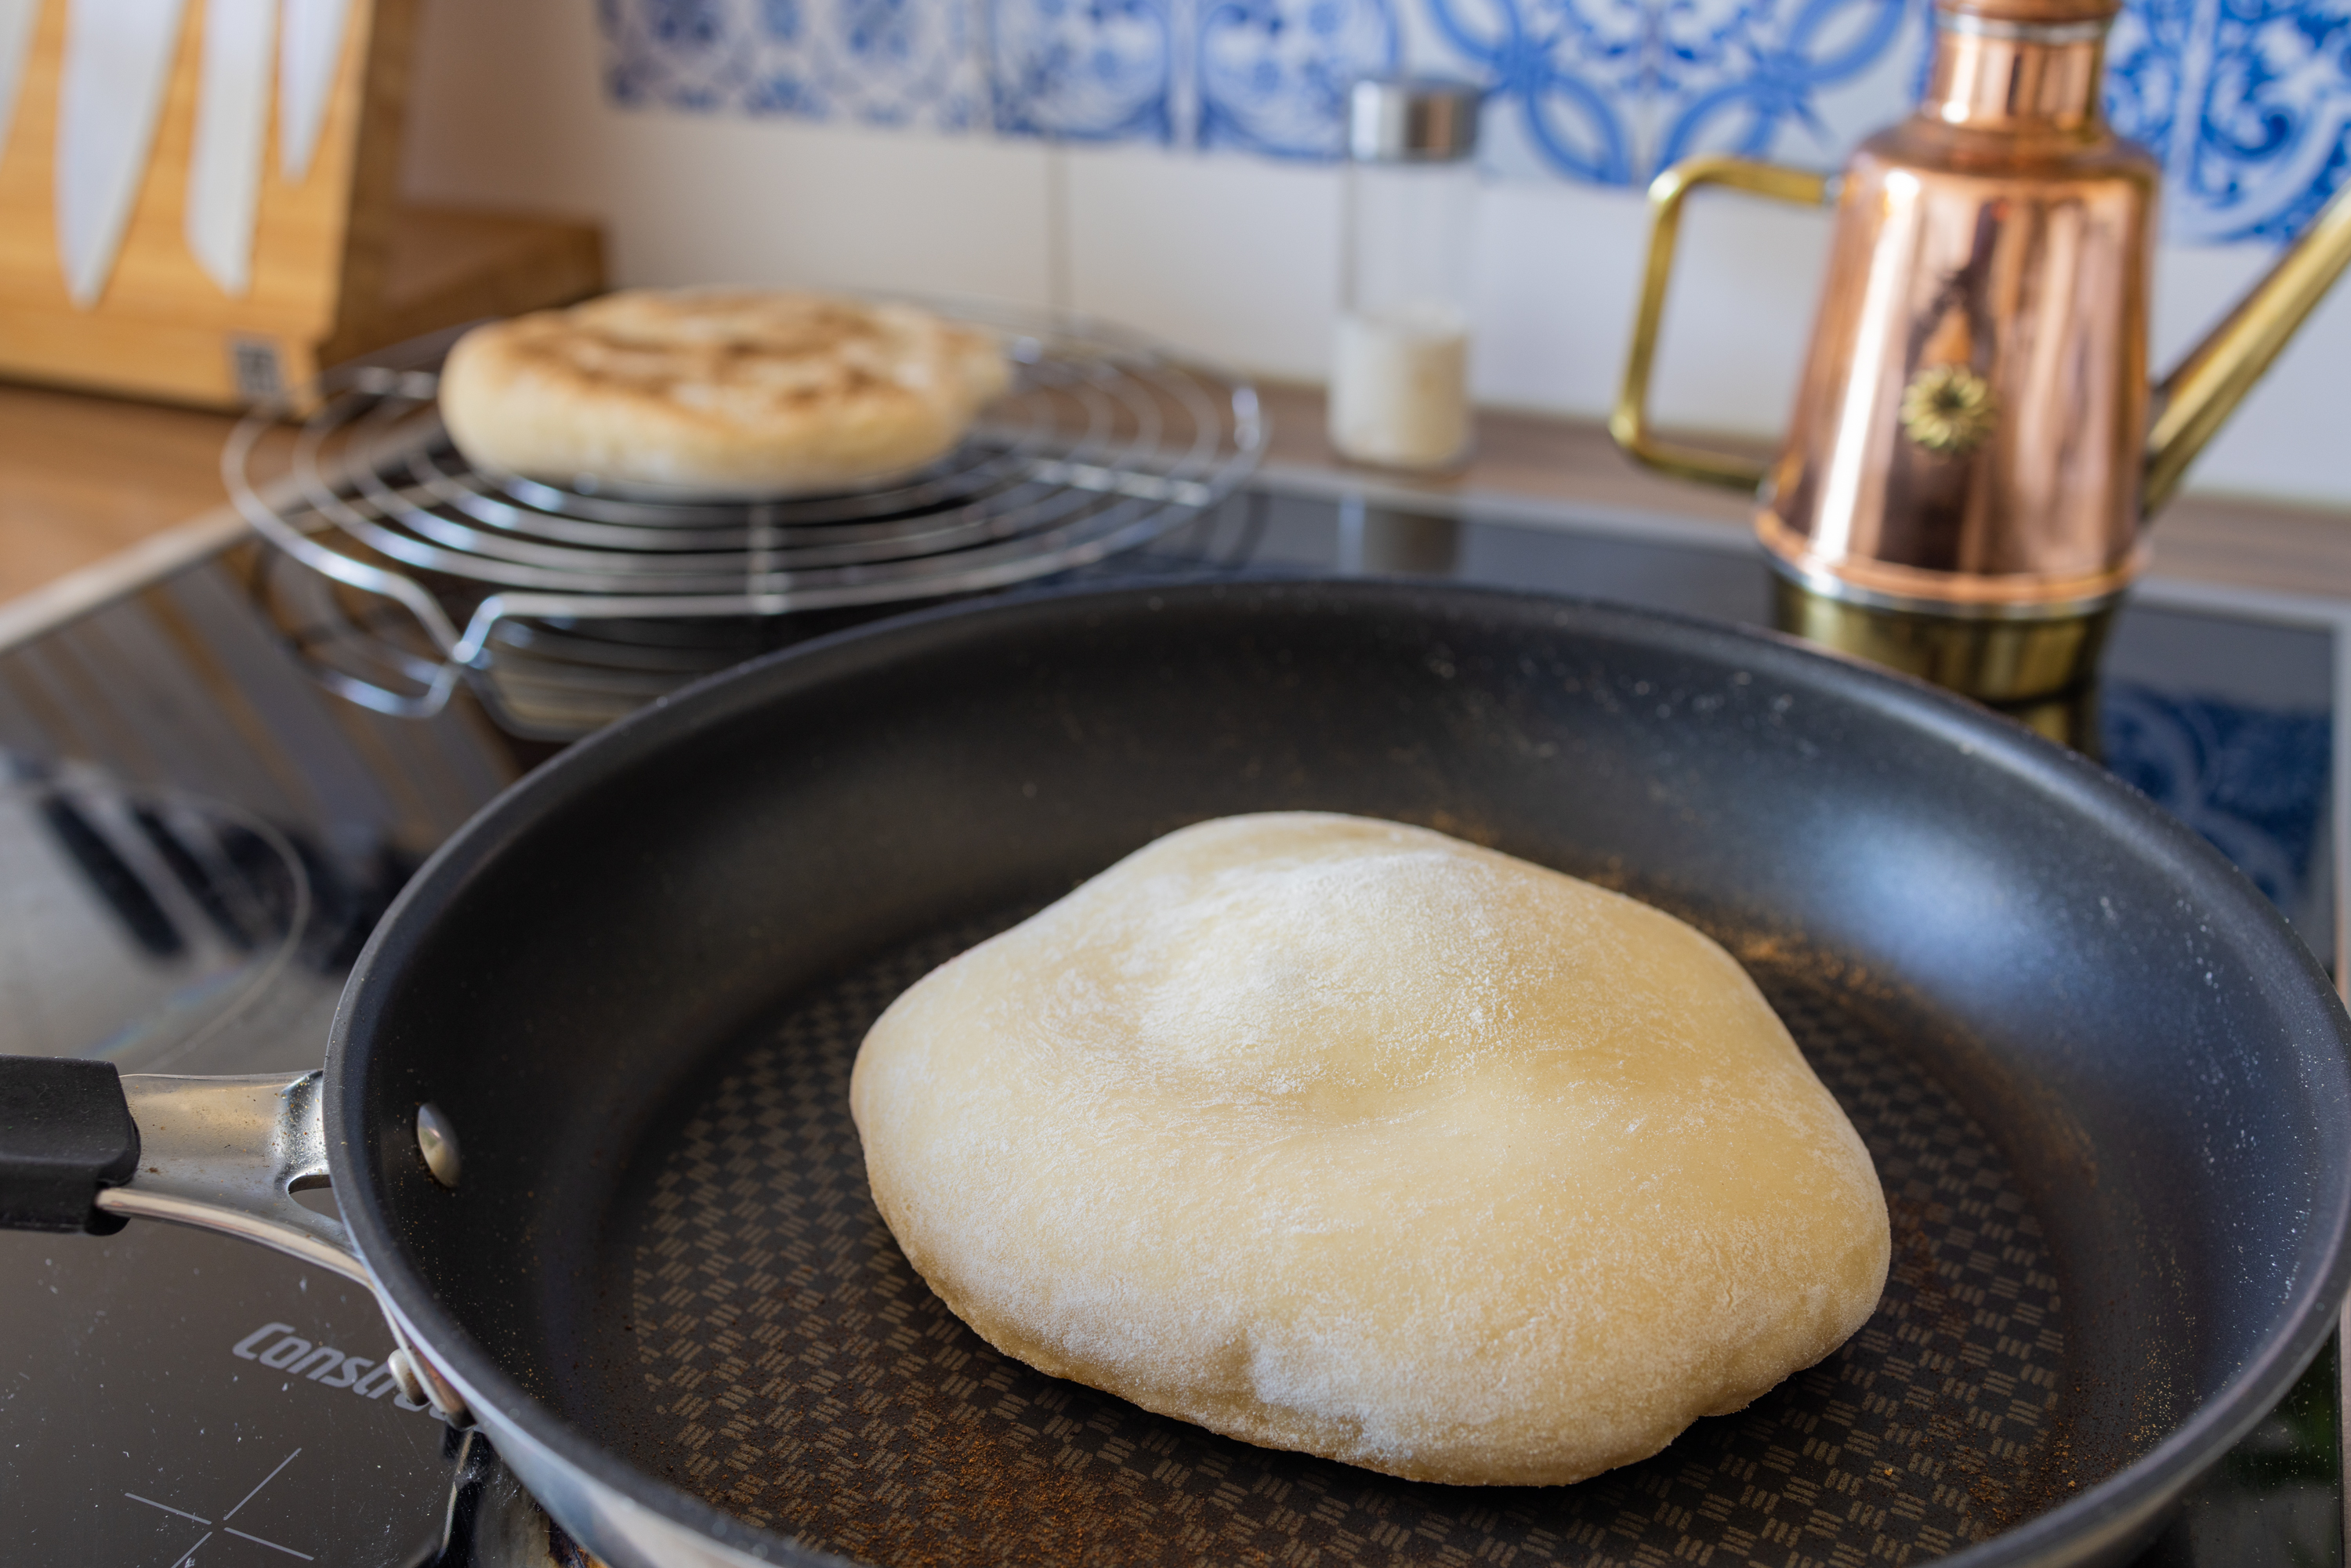
\includegraphics[width=1.0\textwidth]{flat-bread-wheat}
  \caption[Wheat flatbread]{A flatbread made with purely wheat flour. The
      dough is drier at around \qty{60}{\percent} hydration. The drier dough
      is a little harder to mix. As wheat contains more gluten, the dough
      puffs up during the baking process.}
\end{figure}

This way you should have around \qty{11}{\gram} of sourdough ready in the evening. You will have
the perfect quantity to make a dough for one person. In case you want to make more
bread, simply multiply the quantities shown in
Table~\ref{tab:flat-bread-ingredients}.

Then in the evening simply mix the ingredients as shown in the table. Your dough
is going to be ready in the morning. It's typically ready after 6--12~hours. If
you use more sourdough starter it will be ready faster, conversely it will take
longer if you use less. Try to aim for a fermentation time of 8--12~hours as
by using your dough too soon, the flavor might not be as good. By using your
dough later it might become a little more sour. The best option is to
experiment and see what you personally like the most.

After mixing the ingredients together cover the container, this prevents the
dough from drying out and makes
sure no fruit flies get access. A transparent container will be helpful
when getting started. You can observe the dough more easily and see when
it is ready.

\begin{figure}[htb]
\centering
  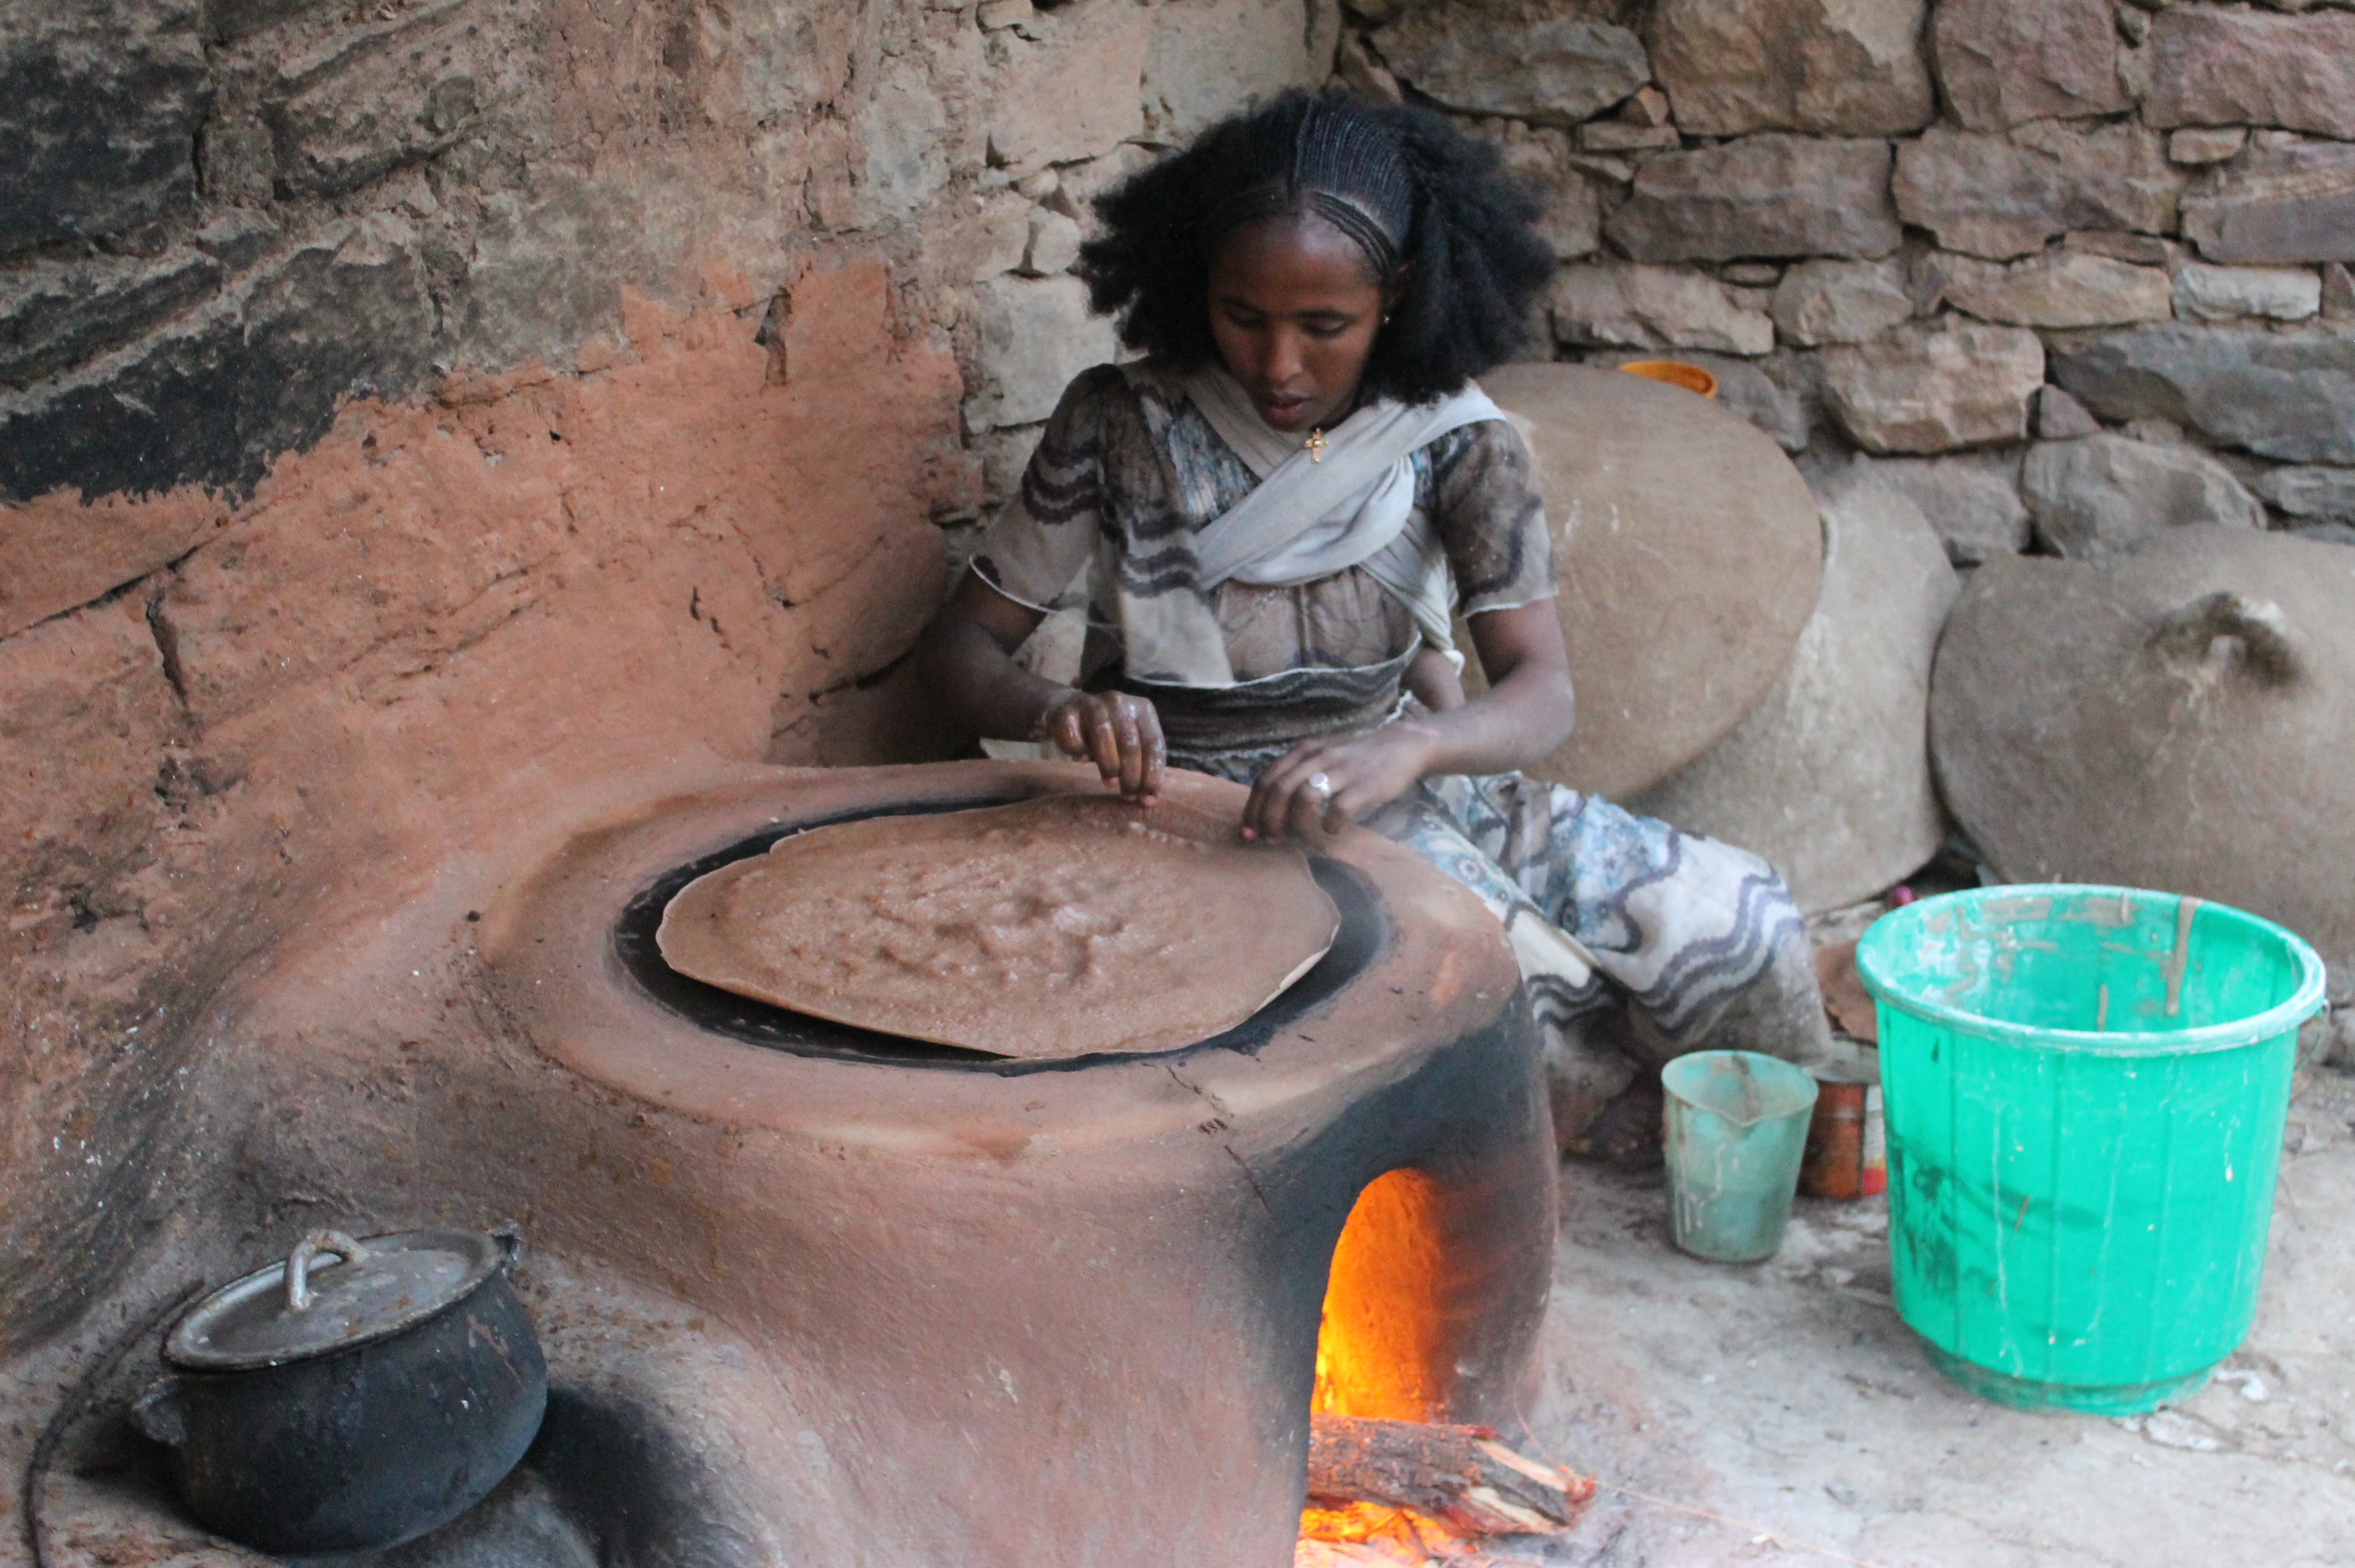
\includegraphics[width=1.0\textwidth]{ethiopian-woman-checking-bread}
  \caption[Ethiopian \emph{injera}]{An Ethiopian woman baking an \emph{injera}
      made using teff flour.  The image has been provided by Charliefleurene
      via Wikipedia.}
\end{figure}

If you used the flatbread option with less water, look at the size increase
of your dough. It should have increased at least \qty{50}{\percent} in size.
Also look out for bubbles on the sides of your container.

When using the pancake recipe, look out for bubbles on the surface of your dough.
In both cases use your nose to check the scent of your dough. Depending
on your sourdough starter's microbiome your dough will have
dairy, fruity, alcoholic notes or vinegary, acetic notes. Relying
on the smell of your dough is the best way to judge whether your
dough is ready or not. Timings are not reliable as they
depend on your starter and the temperature. If your dough
is ready too soon, you can now move it directly to the fridge and bake
it at a later, more convenient time. The low temperature will halt the fermentation
process\footnote{There are some exceptions. In some rare cases your starter
might also work at lower temperatures. You might have cultivated microbes that work best at
low temperatures. Nevertheless, fermentation
is always slower the colder it gets. A fridge really helps to preserve the state
of your dough.}
and your dough will last for several days. The longer you wait, the more sour the
bread is going to be. The fridge is a great option in case you want to
take the dough with you when visiting friends. People are going
to love you for the freshly baked flatbreads or pancakes. If you dare,
you can also taste a little bit of your raw uncooked dough. It is likely
going to taste relatively sour. I~do this frequently to better evaluate the
state of my doughs.

\begin{figure}[!htb]
\centering
  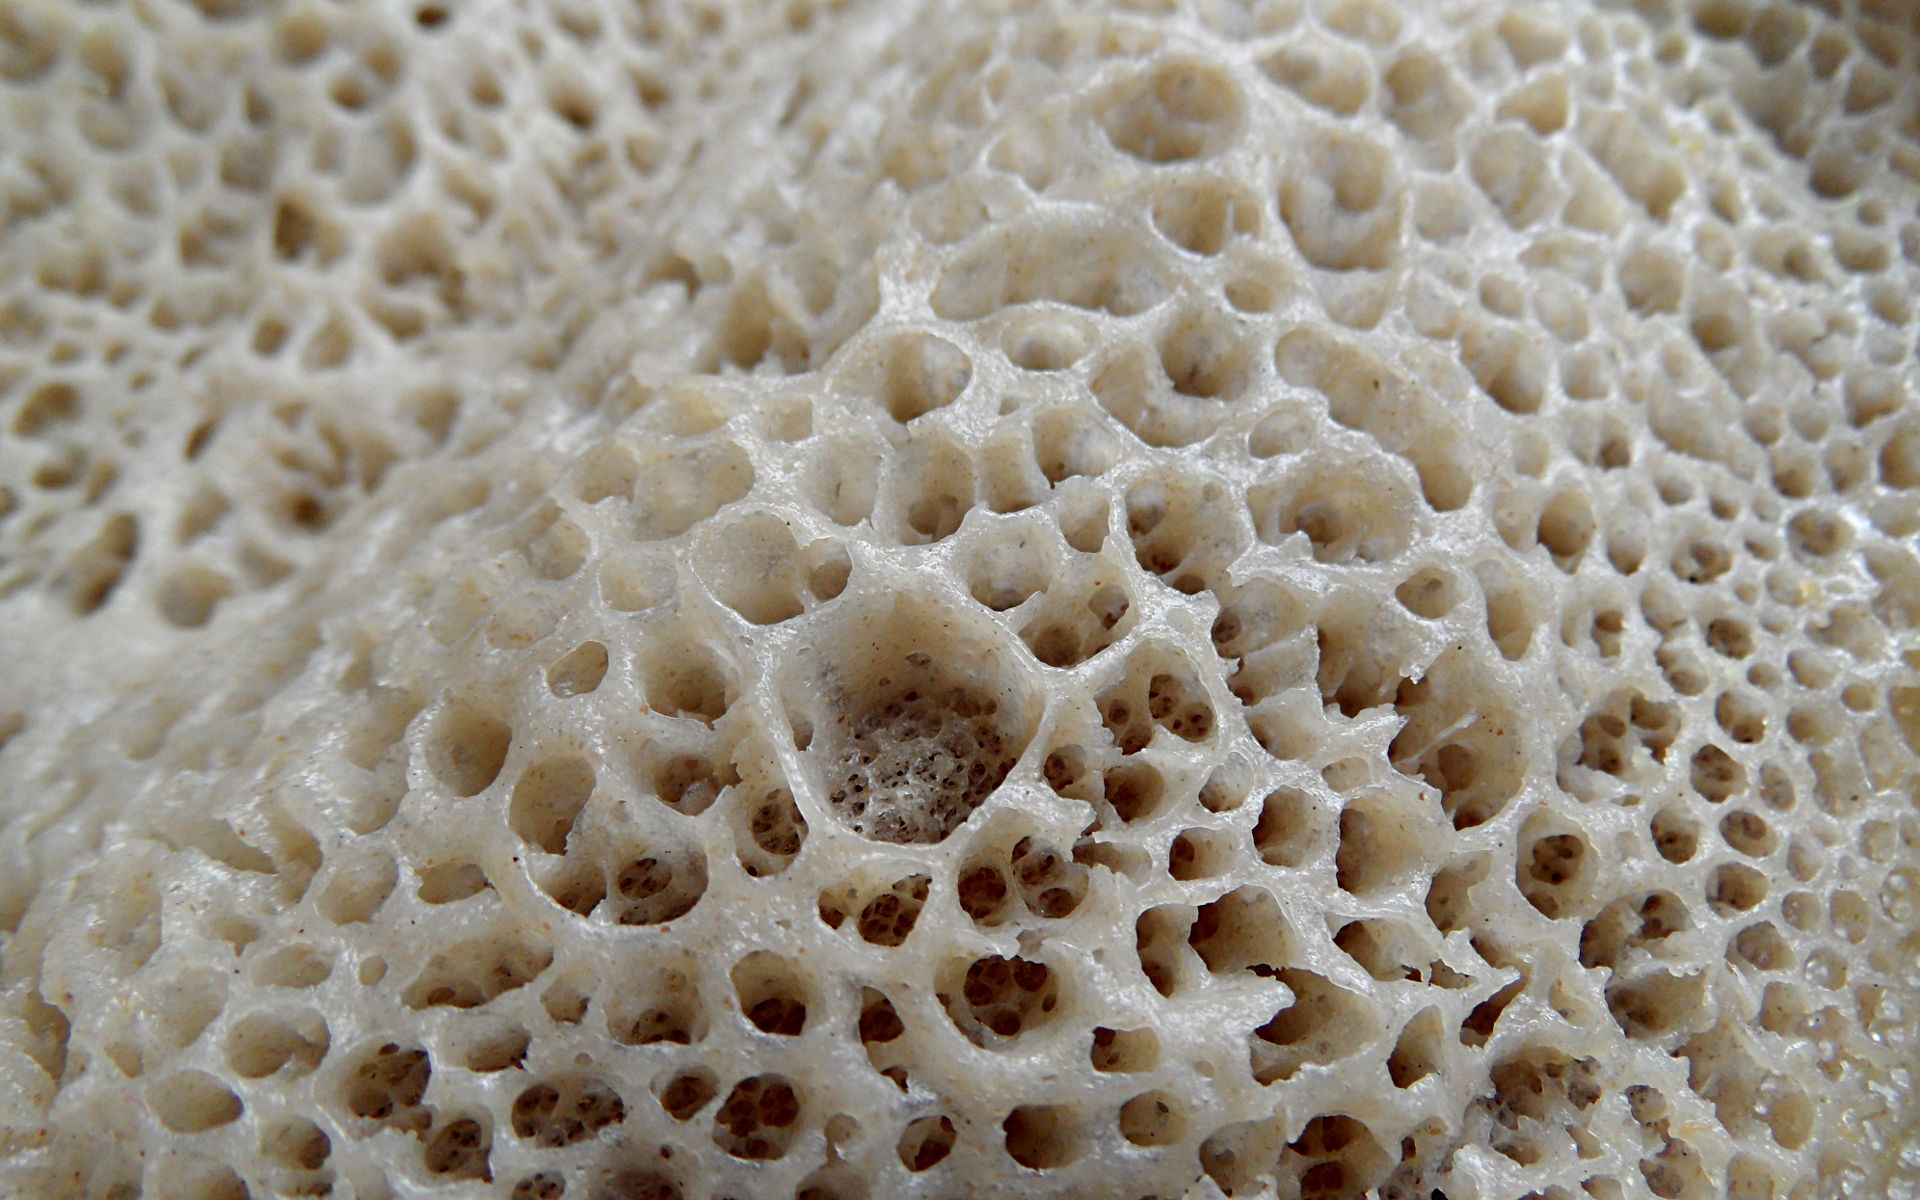
\includegraphics[width=1.0\textwidth]{injera-pancake-texture.jpg}
  \caption[Teff sourdough pancake]{A sourdough pancake made with teff flour.
      The pockets come from evaporated water and \ch{CO2} created by the
      microbes.  The image has been provided by Łukasz Nowak via Wikipedia.}
\end{figure}

If you are feeling lazy or don't have time, you could also use older sourdough starter
to make the dough directly without any prior starter feedings. Your sourdough starter
is going to regrow inside your dough. Remember that the
final bread might be a bit more on the sour side as the balance of yeast to
bacteria could be off. In the Table~\ref{tab:flat-bread-ingredients}
I~recommended using around \qtyrange{5}{20}{\percent}
of sourdough starter based on the flour to make the dough. If you were to follow
this approach, just use around \qty{1}{\percent} and make the dough directly.
The dough is probably going to be ready 24~hours later, depending on the temperature.

If you want to make sweet pancakes, add some sugar and optional eggs to your dough
now. A good quantity of eggs is around one~egg per \qty{100}{\gram} of flour.
Stir your dough a little bit and it will be ready to be used. You'll
have delicious sweet savory pancakes, the perfect combination. By
adding the sugar now, you make sure that the microbes don't have
enough time to fully ferment it. If you had added the sugar
earlier, no sweet flavor would be left  12~hours later.

To bake your dough heat your stove to medium temperature. Add a little bit of
oil to the pan. This helps with heat distribution and ensures even cooking.
With a spatula or a spoon place your dough in the pan. If your dough
was sitting in the fridge, bake it directly. There is no need to wait for your
dough to come to room temperature. If you have a lid,
place it on your pan. The lid helps to cook your dough from the top.
The evaporating water will circulate and heat up the dough's surface. When
making a flatbread, make the dough around \qty{1}{\cm} thick. When using the
pancake option, opt for around \qtyrange{0.1}{0.5}{\cm} depending on what you
like.

\begin{figure}[htb]
\centering
  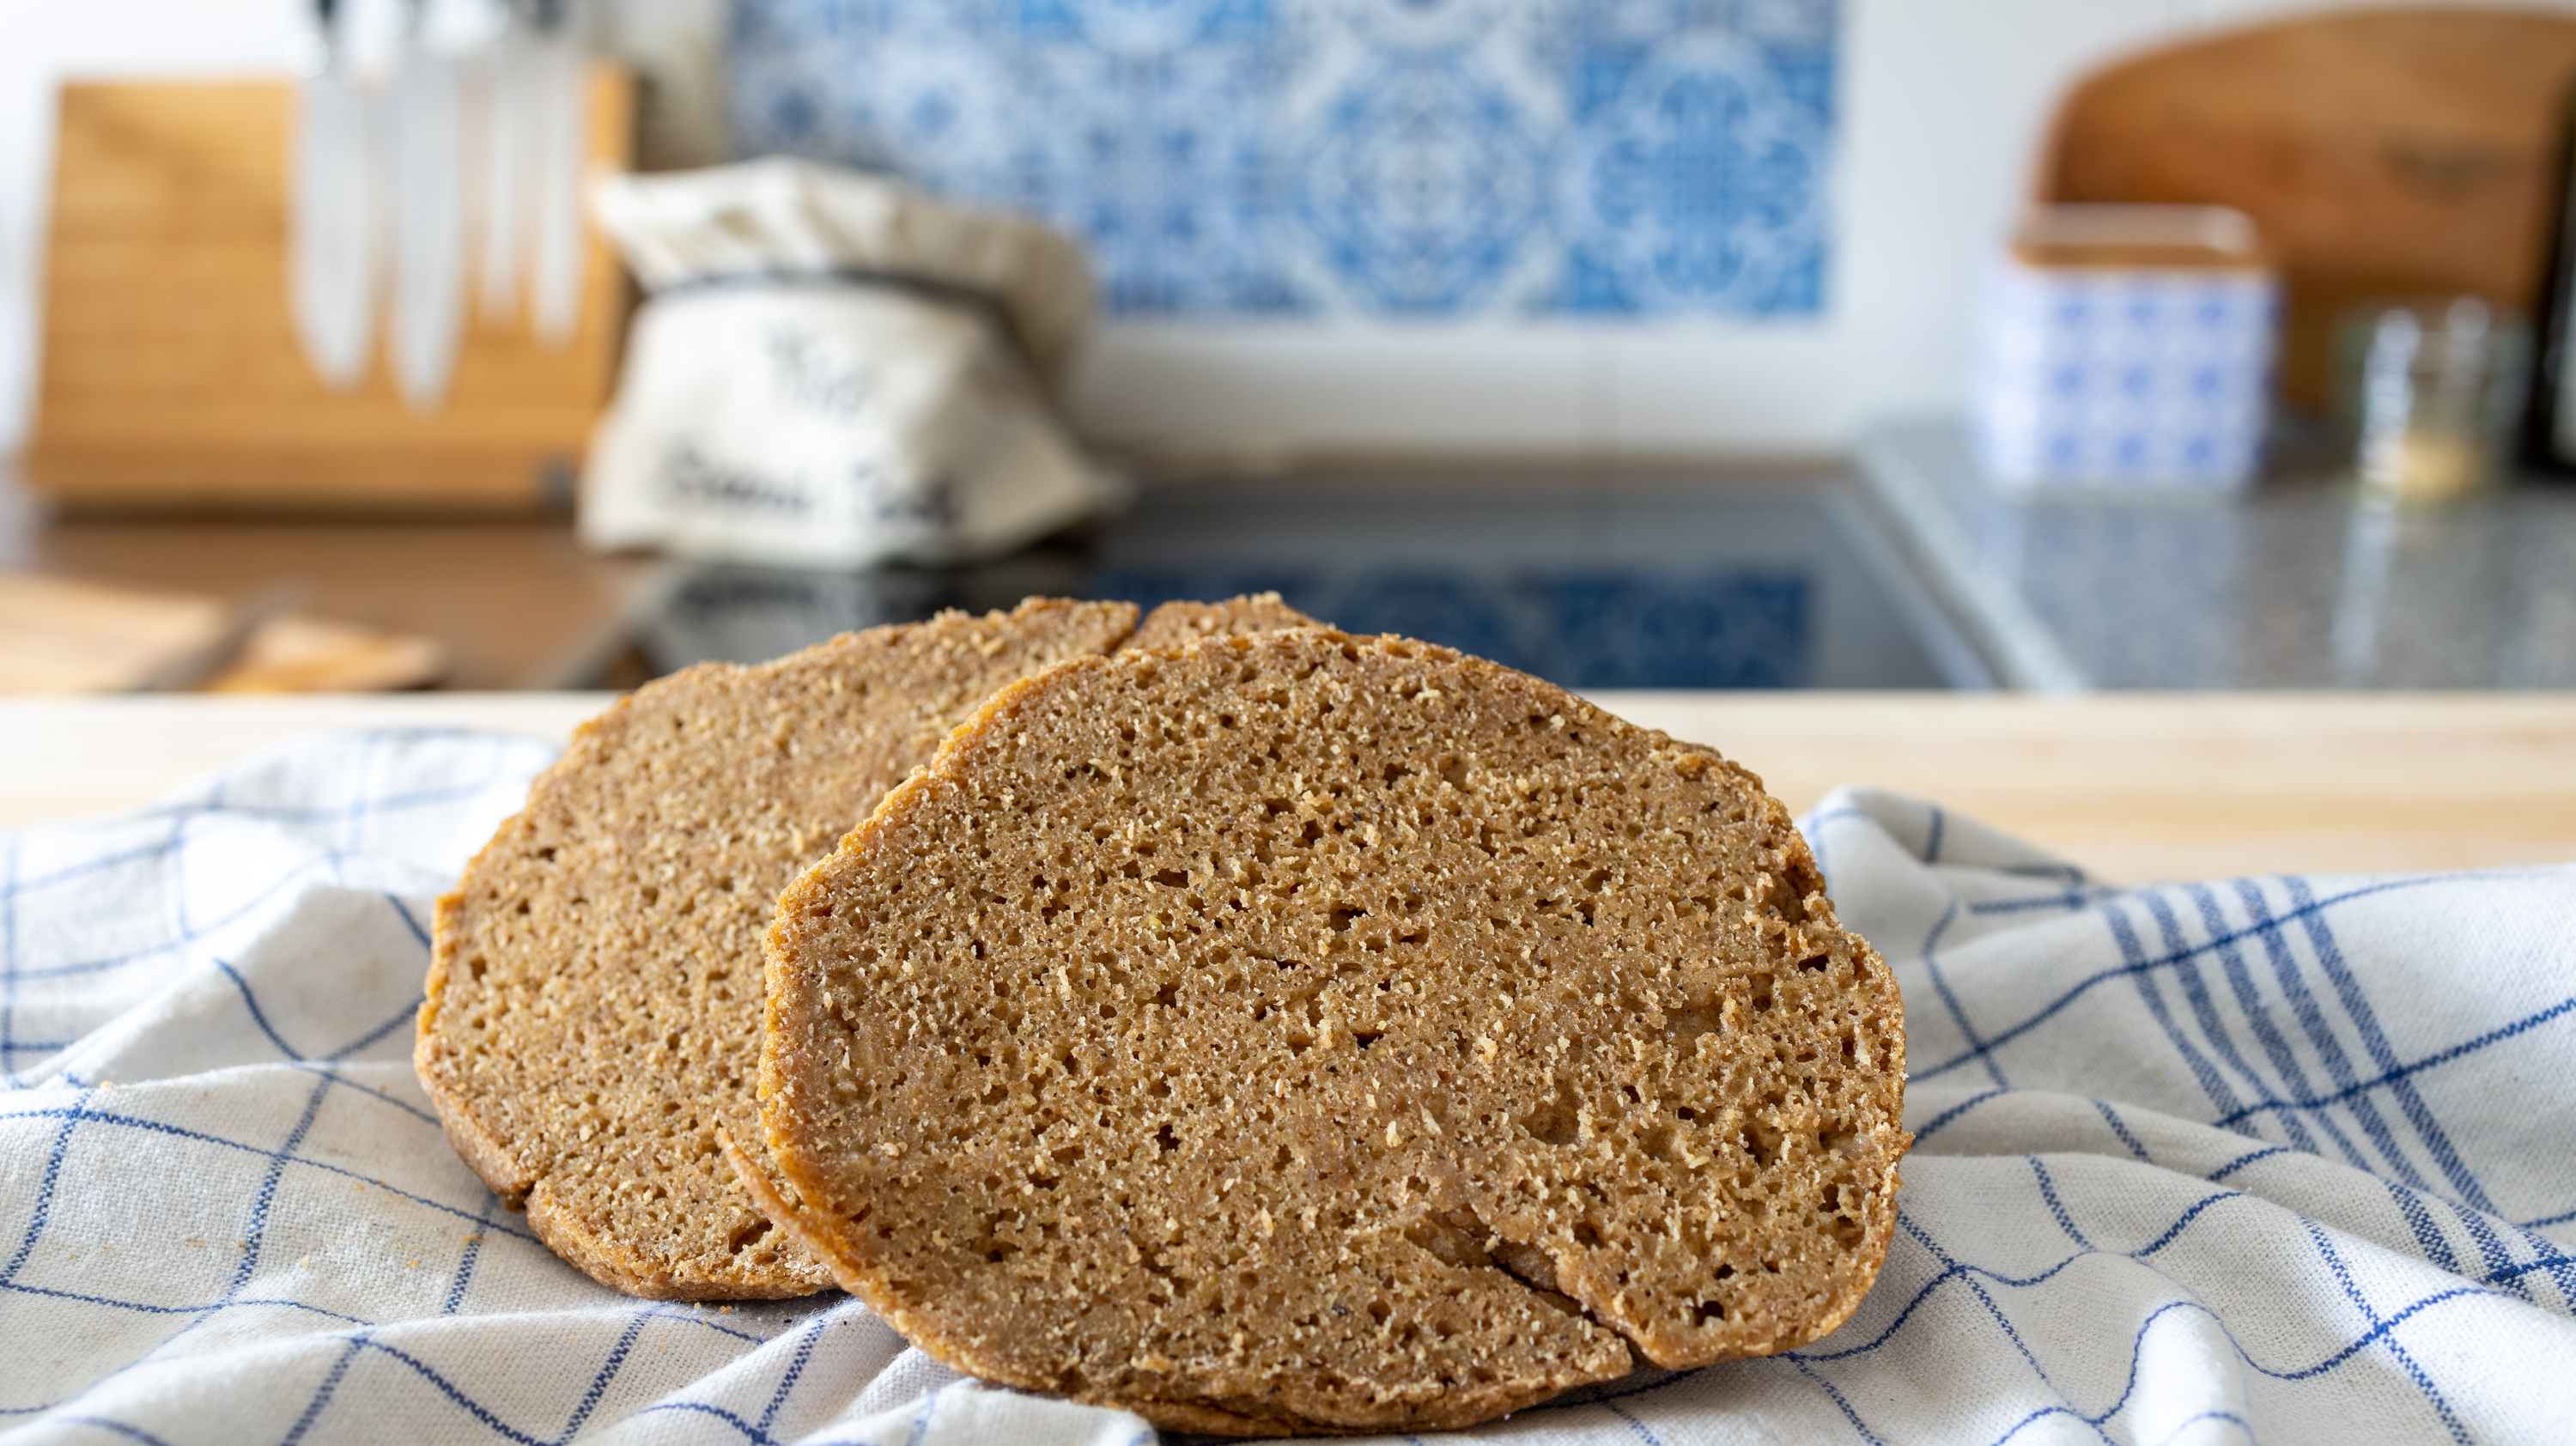
\includegraphics[width=1.0\textwidth]{einkorn-crumb.jpg}
  \caption[Einkorn crum]{The crumb of a flatbread made with einkorn as flour.
      Einkorn is very low in gluten and thus does not trap as much \ch{CO2} as
      a wheat based dough. To make the dough fluffier use more water or
      consider adding more wheat to the mix of your dough.}
\end{figure}

After 2--4~minutes flip over the pancake or flatbread. Bake it for the same
time from the other side. Depending on what you like, you can wait a little
longer to allow the bread to become a bit charred. The longer you
bake your bread, the more of the acidity is going to evaporate. If your
dough is a bit more on the sour side, you can use this trick to balance
out the acidity. This really depends on which flavor you are looking for.

When making a flatbread I~recommend wrapping the baked flatbreads in a kitchen
towel. This way more of the evaporating humidity stays inside of your bread,
making sure your flatbreads stay nice and fluffy for a longer period after the
bake. A similar strategy is used when making corn tortillas.

You can safely store the baked flatbreads or pancakes in your fridge
for weeks. When storing make sure to store them in an airtight plastic bag so that
they do not dry out. If they dry out, spray them with some water and toast them.
They will be almost as good as when they were freshly baked.

Keep a little bit of your unbaked dough. You can use it to make the next
batch of bread or pancakes for the next day. If you want to bake a few days later, add
a little bit of water and flour and store this mixture in your fridge
for as long as you like\footnote{The starter will stay good for months. If you expect to
leave it longer, consider drying a little bit of your sourdough starter.}.

\subsection{Simple flatbread recipe}%
\label{subsec:flat-bread-recipe}

By following the steps outlined in this section,
you'll be introduced to a versatile bread that's perfect for a myriad of
culinary applications. Whether you're scooping up a savory dip,
wrapping a flavorful filling, or simply enjoying a piece with a drizzle
of olive oil, these flatbreads are sure to impress.

\subsubsection*{Ingredients}
\begin{tabular}{r@{}rl@{}}
\qty{400}{\gram} &~(\qty{100}{\percent}) & Flour (wheat, rye, corn, whatever
                                            you have at hand)\\
\qty{320}{\gram} &  (\qty{80}{\percent}) & Water, preferably at room
                                            temperature\\
\qty{80}{\gram}  &  (\qty{20}{\percent}) & Active sourdough starter\\
\qty{8}{\gram}   &   (\qty{2}{\percent}) & Salt\\
\end{tabular}

\subsubsection*{Instructions}
\begin{description}
\item[Prepare the dough] In a large mixing bowl, combine the flour and water.
    Mix until you have a shaggy dough with no dry spots.

    Add the sourdough starter and salt to the mixture. Incorporate them
    thoroughly until you achieve a smooth and homogenized dough.

\item[Fermentation:] Cover the bowl with a lid or plastic wrap. Allow the dough
    to rest and ferment until it has increased by at least \qty{50}{\percent}
    in size.  Depending on the temperature and activity of your starter, this
    can take anywhere from 4 to 24~hours.

\item[Cooking preparation:] Once the dough has risen, heat a pan over medium
    heat.  Lightly oil the pan, ensuring to wipe away any excess oil with a
    paper towel.

\item[Shaping and cooking:] With a ladle or your hands, scoop out a portion of
    the dough and place it onto the hot pan, spreading it gently like a
    pancake.

    Cover the pan with a lid. This traps the steam and ensures even cooking
    from the top, allowing for easier flipping later.

    After about 5~minutes, or when the bottom of the flatbread has a
    golden-brown crust, carefully flip it using a spatula.

    \emph{Adjusting cook time.} If the flatbread appears too dark, remember to
    reduce the cooking time slightly for the next one.  Conversely, if it's
    too pale, allow it to cook a bit longer before flipping.

    Cook the flipped side for an additional 5~minutes or until it's also
    golden brown.

\item[Storing:] Once cooked, remove the flatbread from the pan and place it on
    a kitchen towel. Wrapping the breads in the towel will help retain their
    softness and prevent them from becoming overly crisp.  Repeat the cooking
    process for the remaining dough.

\item[Serving suggestion:] Enjoy your sourdough flatbreads warm, paired with
    your favorite dips, spreads, or as a side to any meal.

\end{description}


\section{Loaf pan bread}%
\label{sec:loaf-pan-bread}

Loaf pan bread is made using the help of a special loaf pan
or loaf tin. The edges of the pan provide additional support
for the dough to rise. Making a bread using a loaf pan requires
an oven.

\begin{figure}[!htb]
  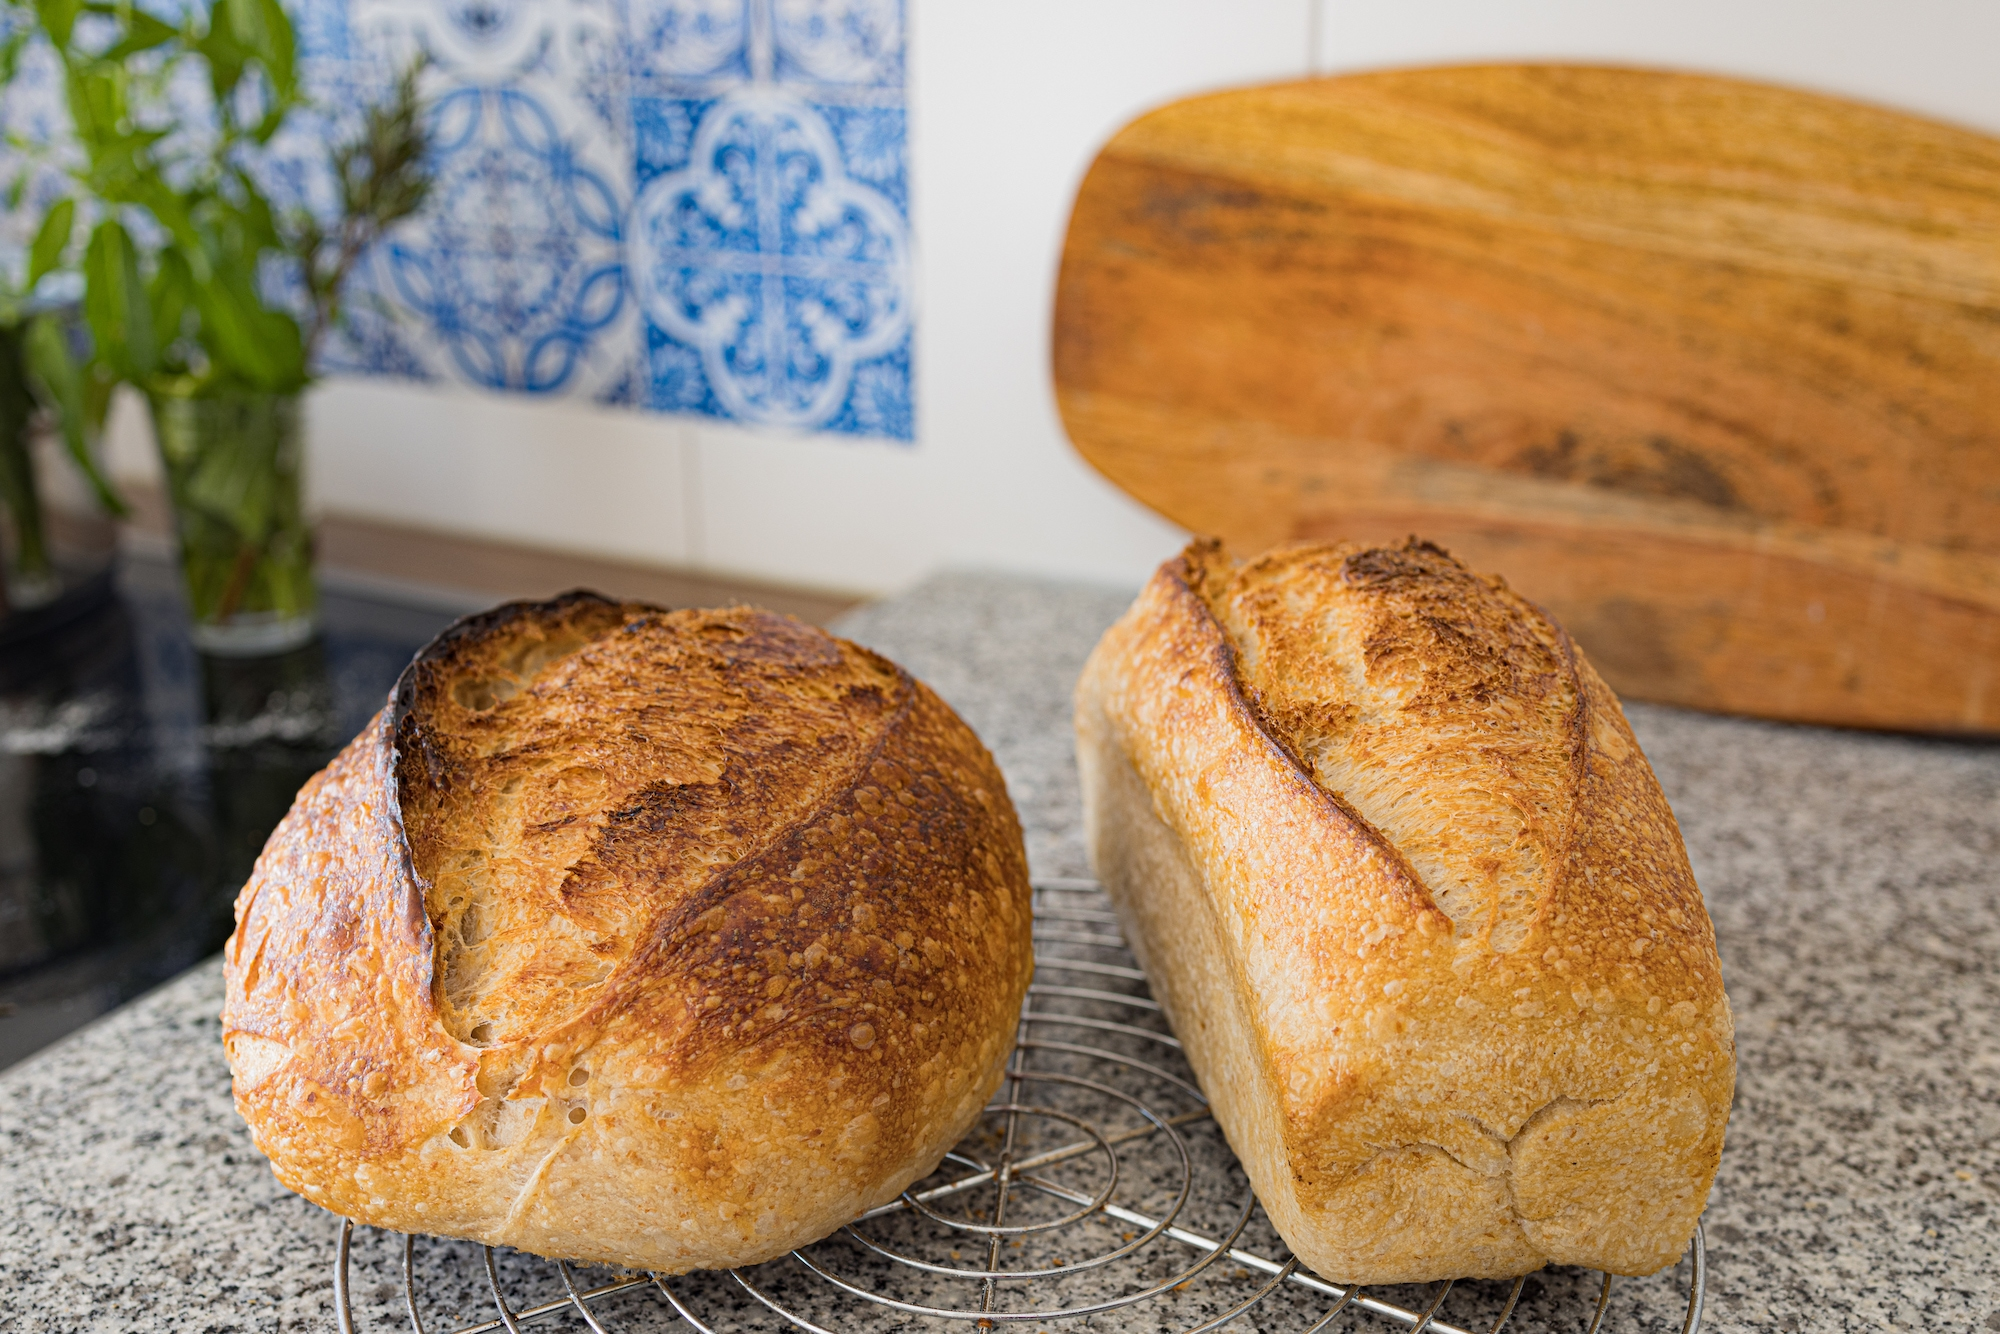
\includegraphics[width=\textwidth]{loaf-pan-free-standing.jpg}
  \caption[Freestanding bread and pan bread]{A freestanding bread and a wheat
      loaf pan bread. Both of them received a small incision before baking
      which helps to control how they open up.}%
  \label{fig:free-standing-loaf-pan}
\end{figure}

After mixing your dough, you can place it directly into the loaf pan.
This makes the whole process simpler since you can skip steps such
as shaping the dough.

To make a great loaf pan bread with little work:

\begin{enumerate}
    \item Mix the ingredients of your dough (gluten free works too)
    \item Place into the loaf pan
    \item Wait until your dough has roughly doubled in size
    \item Bake in a non pre-heated oven for around 30--50~minutes
\end{enumerate}

Knowing the exact baking time is sometimes a little challenging
as it might be that the outside of your bread is cooked but
the inside is still raw. The best way is to use a thermometer
and measure the core temperature. At around  \qty{92}{\degreeCelsius}
(\qty{197}{\degF}) your dough is done. I~generally bake loaf pan bread at
around  \qty{200}{\degreeCelsius} (\qty{390}{\degF}), which is a little less
than my freestanding bread which I~bake at  \qty{230}{\degreeCelsius}
(\qty{445}{\degF}). That's because it takes a while for the dough
to bake properly inside the loaf pan. The edges don't heat up
as quickly. Then the top part of the dough is properly cooked, while
the inside isn't yet. When baking make sure to use steam
or simply place another equally sized loaf pan on top
of your loaf pan. This way you simulate a Dutch oven. The dough's
evaporating moisture will stay inside.

A good trick to make excellent loaf pan bread is to make a very
sticky dough. You can opt for a hydration of \qtyrange{90}{100}{\percent}, almost
resembling a default sourdough starter. Just like with flatbread,
the high humidity helps to make a more airy, fluffy crumb. The bread will
also be a bit chewier. This type of bread made with rye is my family's favorite
style of bread.  The hearty rye flavor paired with the sticky consistency really
makes an excellent sandwich bread.

To improve the structure you can also consider using around \qty{50}{\percent}
wheat flour in your mix. The gluten network will develop as your
dough ferments and allow for more gas to be trapped in the dough.

A common problem you will face when making a loaf pan bread is
the dough sticking to the pan. Use a generous amount of oil to grease
your pan. A nonstick vegetable oil spray can do wonders.
Don't clean your loaf pans with soap. Just use a kitchen towel
to clean them. With each bake a better patina forms, making your
pan more and more stick resistant.

What's amazing about this type of bread is that it works
with every flour. The overall time to work the dough is probably
less than 5~minutes, making it very easy to integrate
into your daily routine. Furthermore, loaf pans use the space
in your oven very efficiently. Using pans I~can
easily bake 5 loaves at the same time in my home oven.
Normally I~would need multiple baking sessions for
freestanding loaves.

\section{Free standing bread}

A freestanding loaf is baked entirely without supporting
baking vessels in your oven. To make a freestanding loaf more steps
and tools are required.

\begin{figure}[!htb]
\centering
  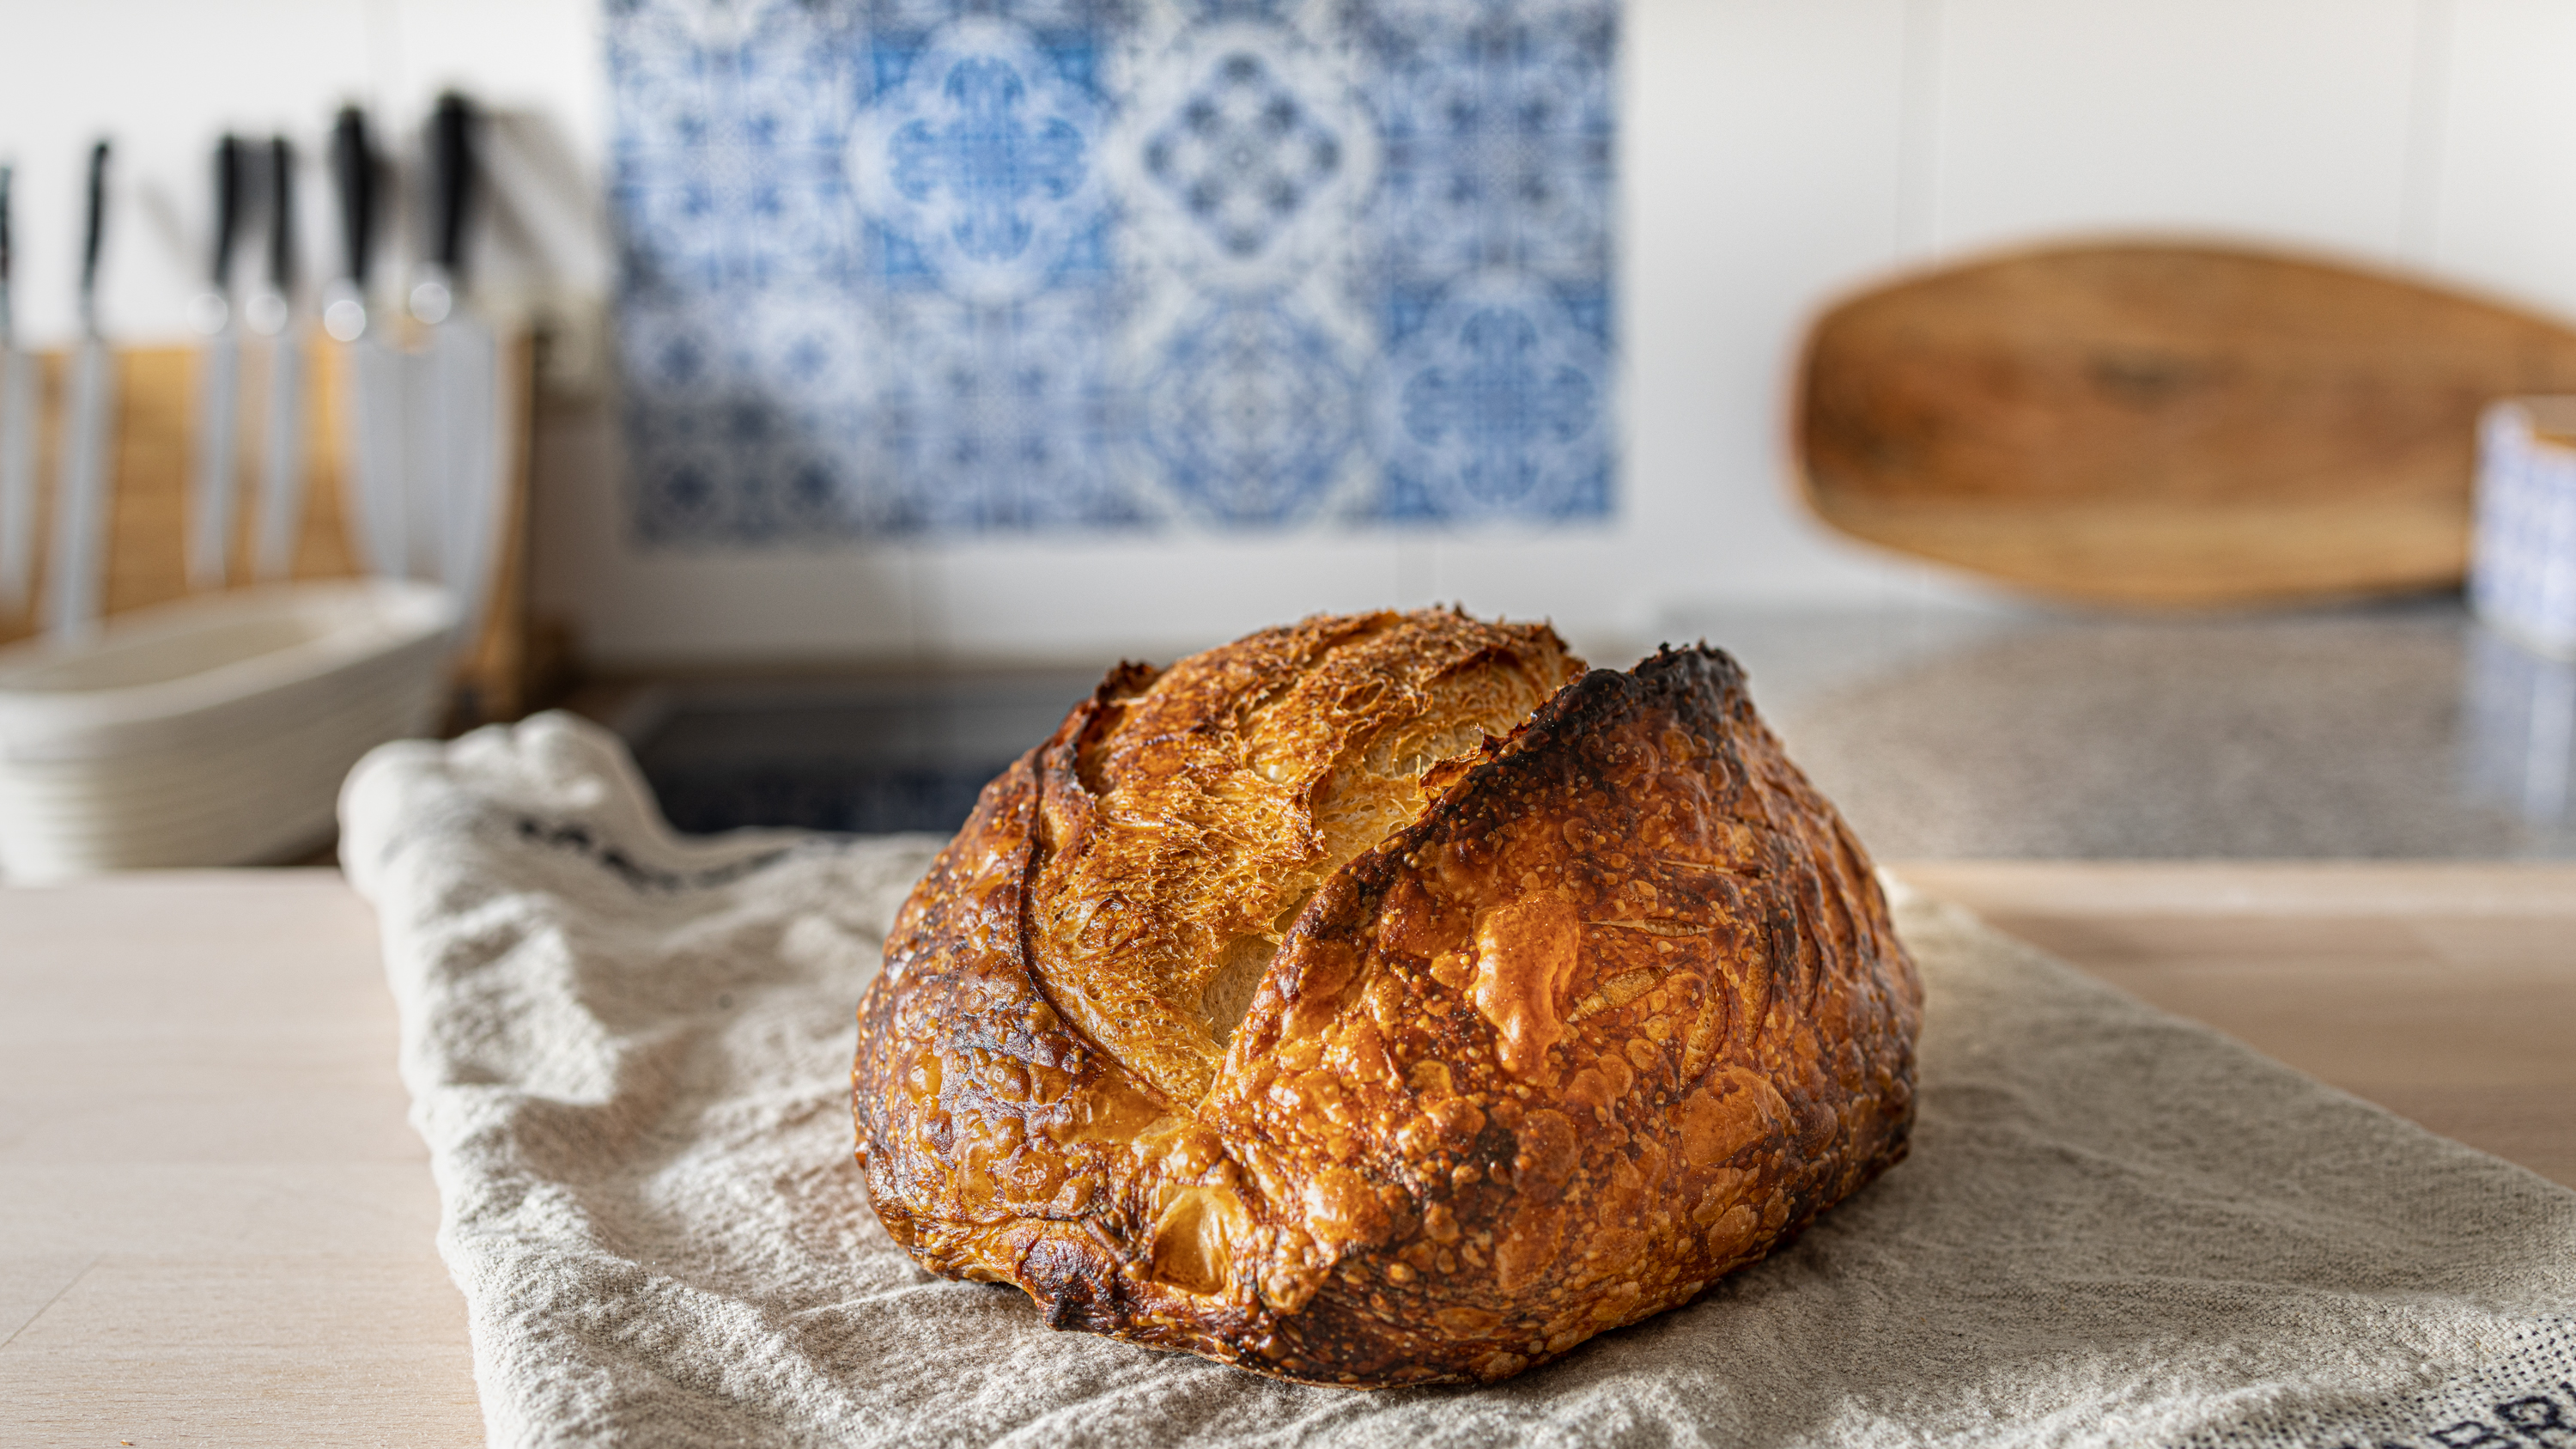
\includegraphics[width=1.0\textwidth]{free-standing-loaf.jpg}
  \caption[Freestanding sourdough bread]{A freestanding sourdough bread. Note
      the incision known as an \emph{ear} and the oven spring clearly
      distinguish this type of bread from flatbread and loaf pan bread.}
\end{figure}

When using wheat, make sure to mix your dough enough to develop a gluten network.
Allow the dough to reach a certain size increase during the fermentation.
Afterward, divide and pre-shape the dough into the desired visual shape you
would like. Each shape requires a different technique. Sometimes achieving
the right shape can be challenging. Making a baguette, for instance,
requires performing more steps. Mastering this technique takes several attempts.

Once the dough is shaped, it is proofed again for a certain
period of time. Once the dough is ready, a sharp tool such
as a razor blade is used to make an incision into the dough.
This helps control how the dough opens up during the baking process.

All these steps require practice. Each of them has to be
performed perfectly, without mistakes.
But after baking you will be rewarded with a beautiful bread
with great taste and consistency.

There is a dedicated recipe and tutorial for this type of bread in the
\nameref{chapter:wheat-sourdough} chapter.


\chapter{Wheat sourdough}%
\label{chapter:wheat-sourdough}
\begin{quoting}
In this chapter, you will learn how to make
freestanding wheat sourdough bread.
\end{quoting}

\begin{figure}[!htb]
  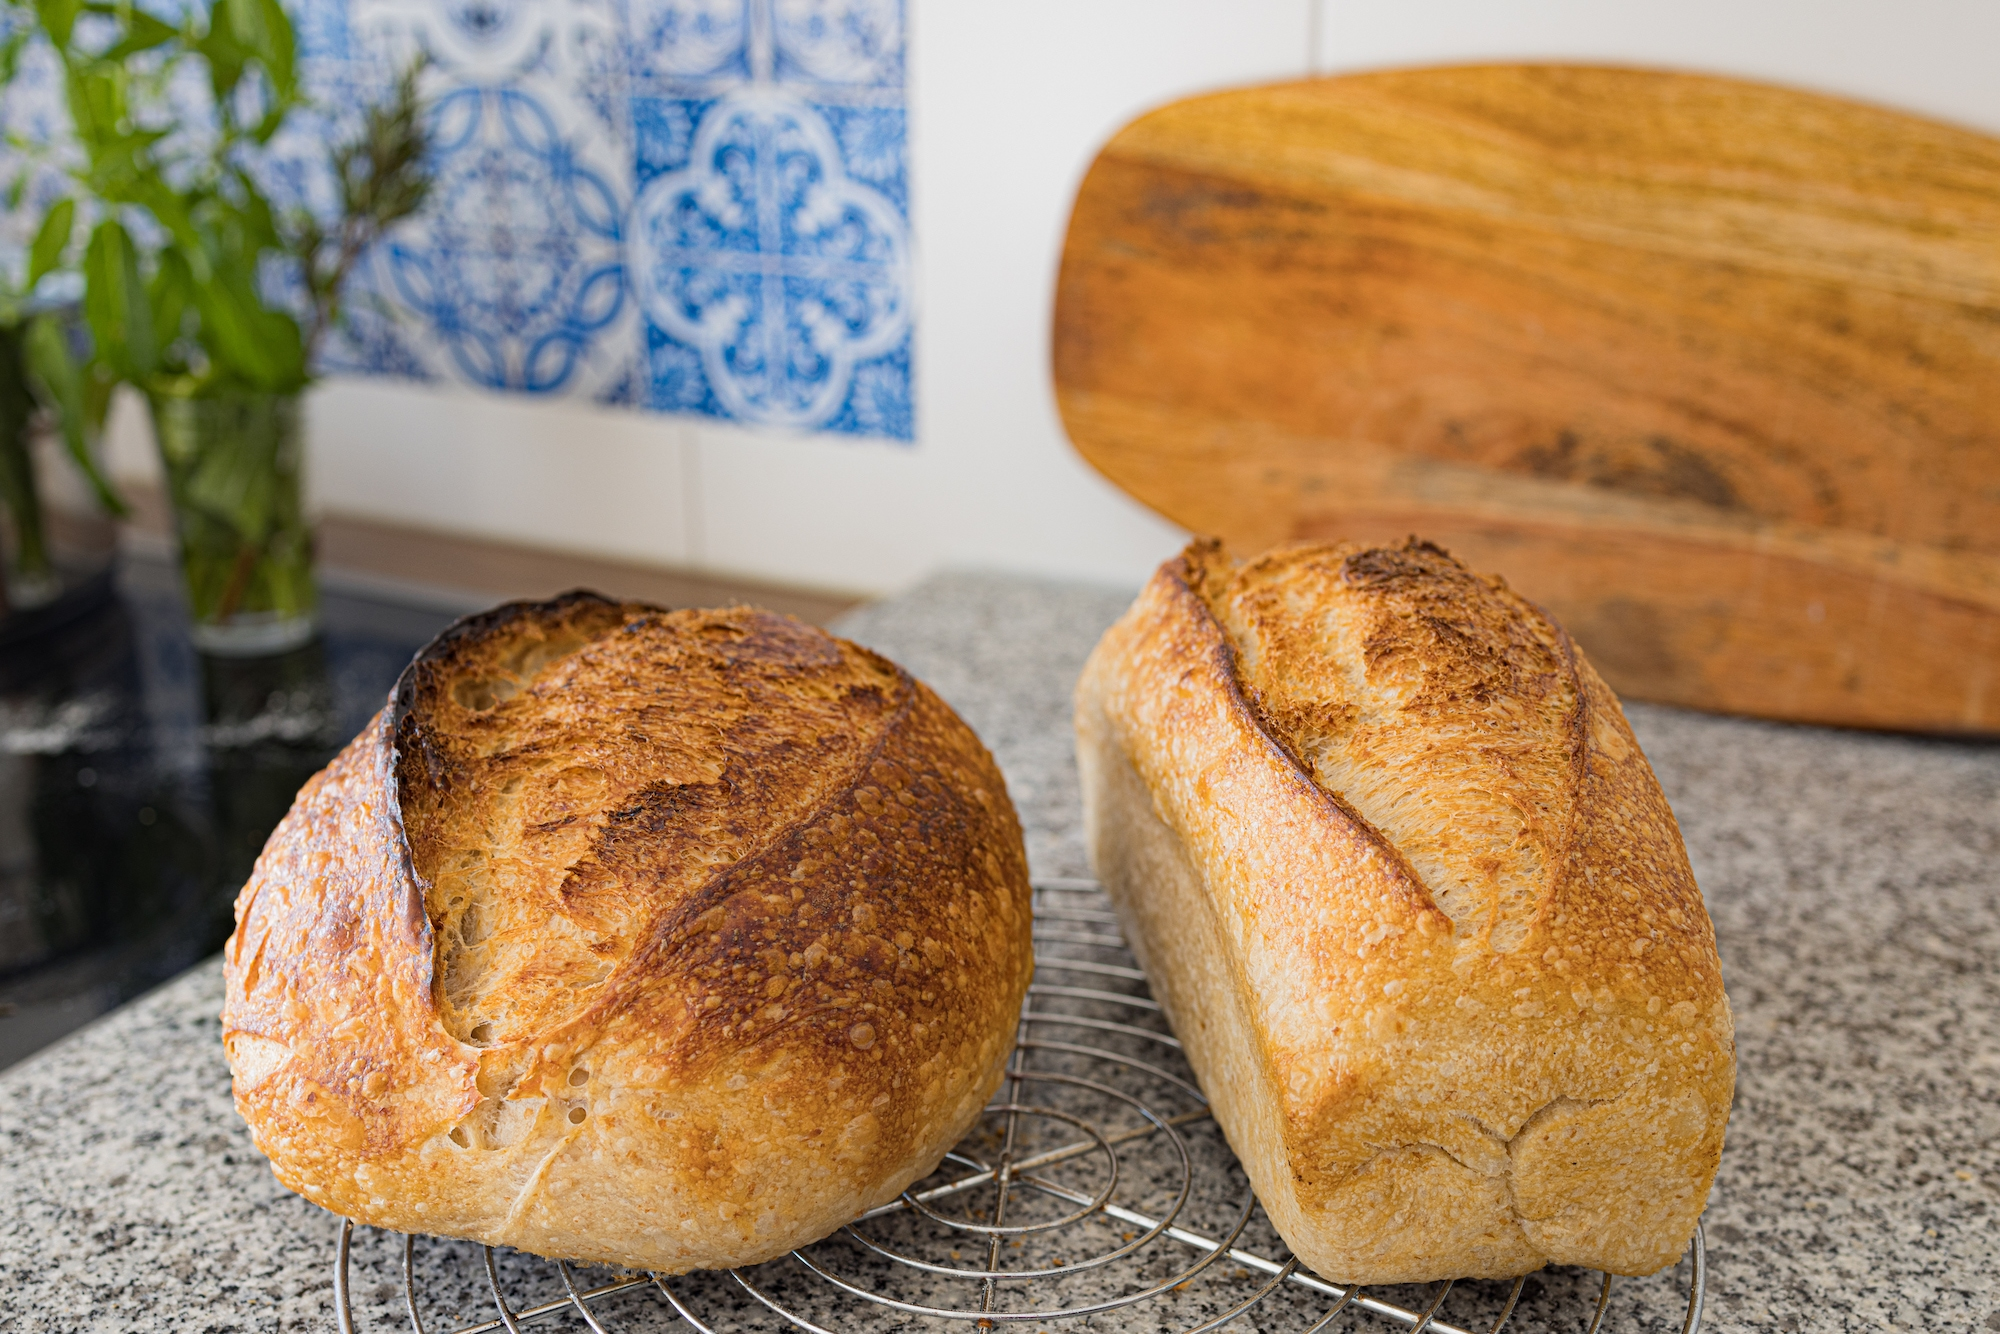
\includegraphics[width=\textwidth]{loaf-pan-free-standing.jpg}
  \caption[Freestanding and loaf pan bread]{A freestanding sourdough bread
      next to bread made in a loaf pan.  Freestanding sourdough is considered
      the supreme discipline of sourdough bread by many bakers.}
\end{figure}

Freestanding sourdough bread is my favorite
type of bread. It combines a great crunchy crust, superb
flavor, and a soft fluffy crumb. This is the type of bread
that is being inhaled by my friends and family. Unfortunately,
making this type of bread requires a lot more effort, patience,
and technique than other types of bread. You have to perfectly
balance the fermentation process. You cannot ferment for too
short and also not for too long. The techniques you need to
learn also require a bit more skill. It took me several attempts
to get this right. I faced several challenges: I~had the wrong flour.
I~didn't properly know how to use my oven.
When should I~stop the fermentation? There is a lot of information
out there. I~dug through most of it and have tried almost everything.
In many cases the information was wrong; in other cases, I~found another
valuable puzzle piece. Aggregating all this
information was one of my main motivations to start \texttt{The Bread Code}.
My key learning was that there is no recipe that
you can blindly follow. You will always have to adapt the recipe
to your locally available tools and environment.

But do not worry. After reading this chapter you will know
all the signs to look out for. You will be able to read your dough.
You will turn into a confident hobby baker who can bake bread
at home, at high altitudes, at low altitudes, in summer, in winter,
at your friend's place, and even on vacation. Furthermore,
you will know how to scale your production from 1 loaf to 100 loaves of bread.
If you ever wanted to open up a bakery, consider this knowledge to
be your foundation.

Mastering this process will enable you to make amazing bread
that tastes much better than any store-bought bread.

\section{The process}

\begin{flowchart}[!htb]
  \centering
  \begin{tikzpicture}[node distance = 3.2cm, auto]
  \node [start] (init) {Ready starter};
  \node [block, right of=init] (mix_ingredients) {Mix ingredients};
  \node [block, right of=mix_ingredients] (dough_strength) {Create dough strength};
  \node [block, right of=dough_strength] (bulk) {Bulk ferment};
  \node [decision, below of=bulk] (divide_test) {Making one loaf?};
  \node [block, right of=divide_test] (divide) {Divide};
  \node [block, below of=divide] (preshape) {Preshape};
  \node [block, below of=divide_test] (shape) {Shape};
  \node [block, left of=shape] (proof) {Proof};
  \node [success, left of=proof] (bake) {Bake};
  \path [line] (init) -- (mix_ingredients);
  \path [line] (mix_ingredients) -- (dough_strength);
  \path [line] (dough_strength) -- (bulk);
  \path [line] (bulk) -- (divide_test);
  \path [line] (divide_test) -- node{yes} (shape);
  \path [line] (divide_test) -- node{no} (divide);
  \path [line] (divide) -- (preshape);
  \path [line] (preshape) -- (shape);
  \path [line] (shape) -- (proof);
  \path [line] (proof) -- (bake);
\end{tikzpicture}

  \caption{The typical process of making a wheat-based sourdough bread.}%
  \label{fig:wheat-sourdough-process}
\end{flowchart}

The whole process of making great sourdough bread starts with
readying your sourdough starter. The key to mastering
this process is to manage the fermentation process properly.
For this, the basis is to have an active and healthy
sourdough starter.

Once your starter is ready, you proceed to mix all the ingredients.
You want to homogenize your sourdough starter properly. This
way you ensure an even fermentation across your whole dough.

After a short break, you will proceed and create dough strength.
Kneading will create a strong gluten network. This is essential
to properly trap the \ch{CO2} created during the fermentation.

Once you've kneaded, the bulk fermentation starts. It is called bulk fermentation
because you typically ferment multiple loaves together in one bulk.
Understanding when to stop this step will take some practice.
But nothing to worry about, you will learn the exact signs to look out for.

Once this is completed you need to divide your large blob of
dough into smaller pieces and pre-shape each piece. This allows
you to apply more dough strength and shape more uniform loaves.

The proofing stage follows where you finish the fermentation process.
Depending on your time you can proof it at room temperature or in the fridge.
Mastering proofing will turn your good loaf into a great loaf.

Lastly, you will finish the whole process by baking. You will learn different
options on how to properly steam your dough. This way your
dough will have a beautiful oven spring. During the second
stage of the baking process, you will finish building your crust.

All the steps rely on each other. You will need to get each of
the steps right to make the perfect bread.

\section{Readying your starter}%
\label{section:readying-starter}

The most crucial part of the bread-making process is your starter.
The starter is what starts the fermentation in your main dough.
If your starter is off, then your main dough is also going
to cause trouble during the fermentation. Your starter's
properties are passed on to your main dough. If your starter
doesn't have a good balance of yeast to bacteria, neither will your
main dough.

\begin{flowchart}[!htb]
\centering
  \documentclass[tikz]{standalone}
\usepackage{tikz}
\usepackage{siunitx}
\DeclareSIUnit\degF{\text{°}F}

\begin{document}
\begin{tikzpicture}[node distance = 3cm, auto]
  \node [block] (init) {\footnotesize Make a starter};
  \node [block, right of=init, node distance=3cm] (feed) {\footnotesize Feed your starter};
  \path [line] (init) -- (feed);
  \node [block, right of=feed, node distance=3cm] (wait_12_after_feed) {\footnotesize Wait 12 hours};
  \path [line] (feed) -- (wait_12_after_feed);
  \node [block, right of=wait_12_after_feed, node distance=3cm] (ready_question) {\footnotesize Perform readiness check};
  \path [line] (wait_12_after_feed) -- (ready_question);
  \node [block, below of=feed, node distance=3cm] (wait_12) {\footnotesize Wait 12 hours};
  \path [line] (wait_12) -- (feed);
  \node [decision, right of=ready_question, node distance=3.5cm] (is_bubbly) {\footnotesize Bubbly? Size Increase?};
  \path [line] (ready_question) -- (is_bubbly);
  \path [line] (is_bubbly) -- node{no} (wait_12);
  \node [decision, below of=is_bubbly, node distance=4.0cm] (check_smell) {\footnotesize Vinegary, or yogurt smell?};
  \path [line] (is_bubbly) -- node{yes} (check_smell);
  \node [block, below of=init, node distance=6cm] (make_dough) {\footnotesize Make your dough};
  \path [line] (check_smell) -- node{yes} (make_dough);
  \path [line] (check_smell) -- node{no} (wait_12);
\end{tikzpicture}
\end{document}

  \caption[Process to prepare your starter before baking]{The process to check
      your sourdough starter when making wheat-based doughs. In practice
      I~frequently use a stiff sourdough starter. The stiff starter features
      enhanced yeast activity. In that case, you can use the same ratios as
      shown in the chart except for the water quantity. The stiff starter has
      a hydration of \qtyrange{50}{60}{\percent}. So you would have half the
      shown water quantities, i.e., if the chart shows \qty{100}{\gram} of
      water, use \qtyrange{50}{60}{\gram} of water for your stiff starter.}%
  \label{fig:process-starter-wheat-sourdough}
\end{flowchart}

Generally, think of the dough you are mixing as a big starter with salt.
After mixing all the ingredients, you have a green field environment again.
The yeast and bacteria start to fight again to outcompete each other.
There is plenty of food available, and they all do their best to win.
Depending on the starter you mix into your dough, some of the microorganisms
might have an advantage over others.

The first option to achieve a good balance is to apply feedings.
If your starter hasn't been fed in a long period, the
bacteria dominate. This happens if your starter has been
sitting unused in the fridge, for instance. As more and more
acidity piles up, the environment is becoming more and more hostile
to the yeast. The lactic acid bacteria tolerate this environment
better. Your dough fermentation would be more on the
bacterial side with this starter. By applying a couple of
feedings, the yeast becomes more active. The older your
starter, the more acid resistant the yeast becomes. Initially,
I~had to feed my starter 2--3 times to fix the balance. With my
more mature starter, one feeding seems to be enough to balance
the microorganisms.

Some people use a 1:1:1 ratio to refresh the starter. This would
be one part of the old starter (\qty{10}{\gram} for instance), 1 part of flour,
and one part of water. I~think this is utter rubbish. As mentioned
your starter is a miniature dough. You would never opt for a 1:1:1 ratio to
make dough. You might use a maximum of \qty{20}{\percent} starter to
make dough. That's why I~advocate using a 1:5:5 ratio or a
1:10:10 ratio depending on how ripe your starter is. As I~almost
always use a stiffer sourdough starter due to its enhanced
yeast fermentation advantages (see Section~\ref{section:stiff-starter})
my ratio is never 1:5:5. My ratio would be 1:5:2.5 (1 part old starter,
5 parts flour, 2.5 parts water). If it is very warm where you live
you could opt for the aforementioned 1:10:5 or 1:20:10. This
way you slow down the ripening of your starter. You can also use this
trick to make starter feeding work with your schedule.
If your starter is typically ready in 6~hours but today you need it
ready later, simply increase how much flour/water you feed your starter.
These are all values that you need to experiment with on your own.
Every starter is unique and might behave slightly differently.

The second option at your disposal is the starter quantity that
you use to make the dough. As previously stated your starter
regrows inside of your main dough. While I~would normally use
\qtyrange{10}{20}{\percent} of starter based on the flour, sometimes I~go
as low as \qty{1}{\percent} starter. This way the microorganisms have
more room to balance out while fermenting the dough. If my sourdough
starter has not been fed in a day, I~might use \qty{5}{\percent} of sourdough
to make a dough. If I~push this to 2 days without feedings,
I~lower the starter amount even further. I~would opt for the
previously mentioned \qty{1}{\percent} starter. If the food is very scarce,
your microorganisms will sporulate. They need to regrow again
from the spores they created. In this hibernation state, it takes
longer for them to become fully active again. I~have tried
several times to make dough directly out of a dry starter.
I~wasn't successful because the fermentation took too long.
The microorganisms had to regrow from spores and then begin
the fermentation. As explained earlier there is a limit to
fermentation times as your dough naturally breaks down.
Furthermore, you want your microorganisms to outcompete
other pathogens contained in the flour. The less starter
you use, the easier it is for them to reproduce. A strong
starter will outcompete other germs. While the method of
reducing the starter works, I~recommend Option 1 more.
It will reliably create better bread. Option 2 is typically
what I~use when I~fed my starter in the morning but didn't
manage to make a dough in the evening. I~don't want to feed
my starter again the next morning. I~would like to make a dough
directly without waiting and thus use less of the very ripe starter.

Over time you will become more accustomed to your starter
and how it behaves. You will be able to read the signs of its
activity and judge its state.

\section{Ingredients}

All you need to make great sourdough bread is flour, water, and salt. You
can of course add additional things to your dough such as seeds. I~personally
enjoy the hearty taste of whole-wheat. Thus I~like to add around
\qtyrange{20}{30}{\percent} of whole-wheat flour to the mix. You could also
make this recipe with \qty{100}{\percent}
whole-wheat flour directly. In this case, look out for strong whole-wheat
flour that is made from flour with higher protein. If you don't like whole-wheat
you can omit the flour from the recipe. Simply replace the listed
quantity with bread flour. One thing to consider about whole-wheat
flour is its increased enzymatic activity. By adding some whole-wheat
flour you will speed up the whole fermentation process.

Especially when getting started I~recommend using bread flour which
contains more gluten than all-purpose or cake flour. This is essential
when trying to bake a freestanding loaf with sourdough.

Find below an example recipe for 1 loaf including baker's math calculation:

\begin{itemize}
  \item \qty{400}{\gram} of bread flour
  \item \qty{100}{\gram} of whole-wheat flour
  % Manual unit so we can use emphasis
  \item \emph{Total: 500~g of flour}
  \item \qtyrange{300}{450}{\gram} of room temperature water (\qty{60}{\percent} up to \qty{90}{\percent}). More on
this topic in the next chapter.
  \item \qty{50}{\gram} of stiff sourdough starter (\qty{10}{\percent})
  \item \qty{10}{\gram} of salt (\qty{2}{\percent})
\end{itemize}

In case you want to make more bread simply increase the quantities based on
how much flour you have. Let's say you have \qty{2000}{\gram} of flour available. The
recipe would look like this:

\begin{itemize}
  \item \qty{1600}{\gram} of bread flour
  \item \qty{400}{\gram} of whole-wheat flour
  % Manual unit so we can use emphasis again
  \item \emph{Total: 2000~g of flour}, equaling 4 loaves
  \item \qty{1200}{\gram} up to \qty{1800}{\gram} of room temperature water (60 to \qty{90}{\percent})
  \item \qty{200}{\gram} of stiff sourdough starter (\qty{10}{\percent})
  \item \qty{40}{\gram} of salt (\qty{2}{\percent})
\end{itemize}

This is the beauty of baker's math. Simply recalculate the percentages, and you
are good to go. If you are unsure about how this works, please check out the
full Section~\ref{section:bakers-math} which looks at the topic in detail.

\section{Hydration}

Hydration refers to how much water you use for your flour. When
beginning to make bread, I~always got this wrong. I~followed a recipe from the
internet, and my dough never looked like the dough shown in the recipe.
The amount of water your flour requires is not fixed. It depends on the flour
you have.

When a seed gets into contact initially, the outer layers soak up the water.
That's why when using whole-wheat (still containing these layers) you have to
use a little bit more water.

By forming gluten strands, water is absorbed into your dough's gluten matrix. The higher the
protein value, the more water can be used.

Some bakers like to use highly hydrated doughs to create fluffier
bread\footnote{Sometimes it almost feels like a comparison of skill value
between bakers. The more water they can handle, the more skillful the baker.}.
The reason for this
is the dough's improved extensibility. The wetter the dough, the easier it is
for the dough to be stretched. When you pull it, the dough will hold its
shape. In comparison, a very stiff (low hydration) dough will maintain its
shape for a longer period. To visualize this, think of your extensible
dough as a balloon. The stiff dough is like a car tire.
The yeast has a much harder time inflating the car tire compared to the balloon.
That’s because the rubber of the car tire is much less extensible.
It requires much more force to inflate the tire. For this reason,
an extensible dough will inflate more in the oven. The loaf will
be visually bigger and offer an airier more open crumb structure.

While this might sound great, the high hydration causes several side effects.

\begin{enumerate}
  \item Your dough becomes more difficult to handle. Your dough will be stickier.
  \item Your dough has to be kneaded for longer to build a proper gluten
    network.
  \item During the fermentation your dough might become too extensible and lose
    some of the dough strength. To circumvent this, stretch and folds are applied
    compared to regular dough,
    requiring you to invest a lot more work.
  \item Shaping becomes much more of a hassle as the dough is very sticky.
  \item The dough can stick to the banneton a lot easier while proofing.
  \item If you wait too long during proofing, the dough won't have enough strength
    left to pull upwards and will stay flat.
  \item Generally, the higher the water content, the more bacterial fermentation you
    have. Thus a wetter dough will reduce gluten faster than a stiffer dough.
    This is why you have to start the fermentation with a sourdough starter in
    perfect shape. Bakers use a process called autolysis to shorten the main
    fermentation time to circumvent this.
  \item The crumb, in the end, might be perceived as somewhat sticky. It still
    contains a lot of water. I~love this crumb, but this comes down to personal
    taste.
\end{enumerate}

To achieve a high-hydration dough, it is best to slowly add water to
your dough. Start with \qty{60}{\percent} hydration, then slowly add a bit more water. Knead
again until the water is absorbed. Repeat and add more water. As your dough
has already formed a gluten network, new water can be absorbed much easier.
You will be surprised by how much water your dough can soak up. This
method is commonly known as the bassinage method. More on that later.
By opting for this technique, I~was easily able to push a low-gluten flour
to a hydration of \qty{80}{\percent}. This
is also my method of choice when making dough now. I~keep adding water until
I~can feel that the dough has the right consistency. As you bake more bread,
you will develop a better look and feel for your dough. When mixing
by hand this can be quite cumbersome. It is a lot easier when using a stand
mixer.

All in all, increasing hydration requires a lot of trial and error. There
is however one option that makes things easier and causes fewer headaches:
Slow fermentation. You get the same extensibility advantages the high hydration
offers by simply letting your dough ferment for a longer period.
Slowing the fermentation process is easy. Use less
sourdough starter or ferment in a cooler environment.

There are two reasons for the slow fermentation advantages.
As explained earlier, both the protease enzyme and bacteria break down your
gluten network. So as fermentation progresses, your dough will automatically
become more extensible. This is because the rubber layers of your car tire
are slowly converted and eaten. Ultimately your car tire turns into a balloon
that can very easily be inflated. When waiting too long, the
balloon will burst. You will have no gluten left anymore, and your dough
becomes very sticky. Finding the sweet spot of enough rubber eating and not
too much is what the perfect wheat sourdough bread is about. But don't worry --- after reading
this chapter you will have the right tools at your disposal.

The advantages of slow fermentation can be nicely observed when experimenting
with a fast-fermenting yeast dough (\qty{1}{\percent} dry yeast based on flour). The
crumb of such a dough is never as
open as a dough made with sourdough. Furthermore, the protease enzyme
cannot do its job within such a short fermentation period.
Large industrial bakeries add active malt which contains a
lot more enzymes. This way the time required to make the dough is shortened. You
will most likely find malt as an ingredient in supermarket bread. It is a
great hack. The baked turbo fermentation bread will feature a relatively dense
and not fluffy crumb. That is because only very little gluten is broken down when
finishing the fermentation period in 1~hour. If you were to slow things down,
the dough would look completely different.
Try this again and use much less yeast. This is the
secret of Neapolitan pizza. Only a tiny bit of yeast is used to make the
dough. My default pizza recipe calls for around \qty{150}{\mg} of dry
yeast per \unit{\kg} of flour. Give it a shot yourself the next time you
make a yeast-based dough. Try to push the fermentation to at least 8~hours.
The difference is incredible. You will have made bread with a much more
fluffy and open crumb. The flavor of the dough is drastically improved. Your
crust becomes crisper and features a better taste. This is because amylases have
converted your starches into simpler sugars which brown better during baking.
If you only learn one thing from this book, it is that slow fermentation is
the key to making great bread.

For this reason, my default hydration is much lower than the hydration of other
bakers. I~prefer slower fermentation for my recipes.
The sweet spot for my default flour is at around \qty{70}{\percent} hydration.
Again, this is a highly subjective value that works for my flour.

If you are just getting started with a new batch of flour,
I~recommend conducting the following test. This will help you to
identify the sweet spot of your flour's hydration capabilities.

Make 5 bowls with each \qty{100}{\gram} of flour. Add different slightly increasing
water amounts to each of the bowls.

\begin{itemize}
  \item \qty{100}{\gram} of flour, \qty{55}{\gram} of water
  \item \qty{100}{\gram} of flour, \qty{60}{\gram} of water
  \item \qty{100}{\gram} of flour, \qty{65}{\gram} of water
  \item \qty{100}{\gram} of flour, \qty{70}{\gram} of water
  \item \qty{100}{\gram} of flour, \qty{75}{\gram} of water
\end{itemize}

Proceed and mix the flour and water mixture until you see that there
are no chunks of flour left. Wait 15~minutes and return to your dough.
Carefully pull the dough apart with your hands. Your dough should be elastic, holding
together very well. Stretch your dough until very thin. Then hold it against a light.
You should be able to see through it. The flour-water mixture that breaks without
seeing the windowpane is your no-go zone. Opt for a dough with
less hydration than this value. You will know that your flour mix can go up to
 \qty{65}{\percent} hydration, for instance. Use the leftovers of this experiment
to feed your starter.


\begin{figure}[!htb]
  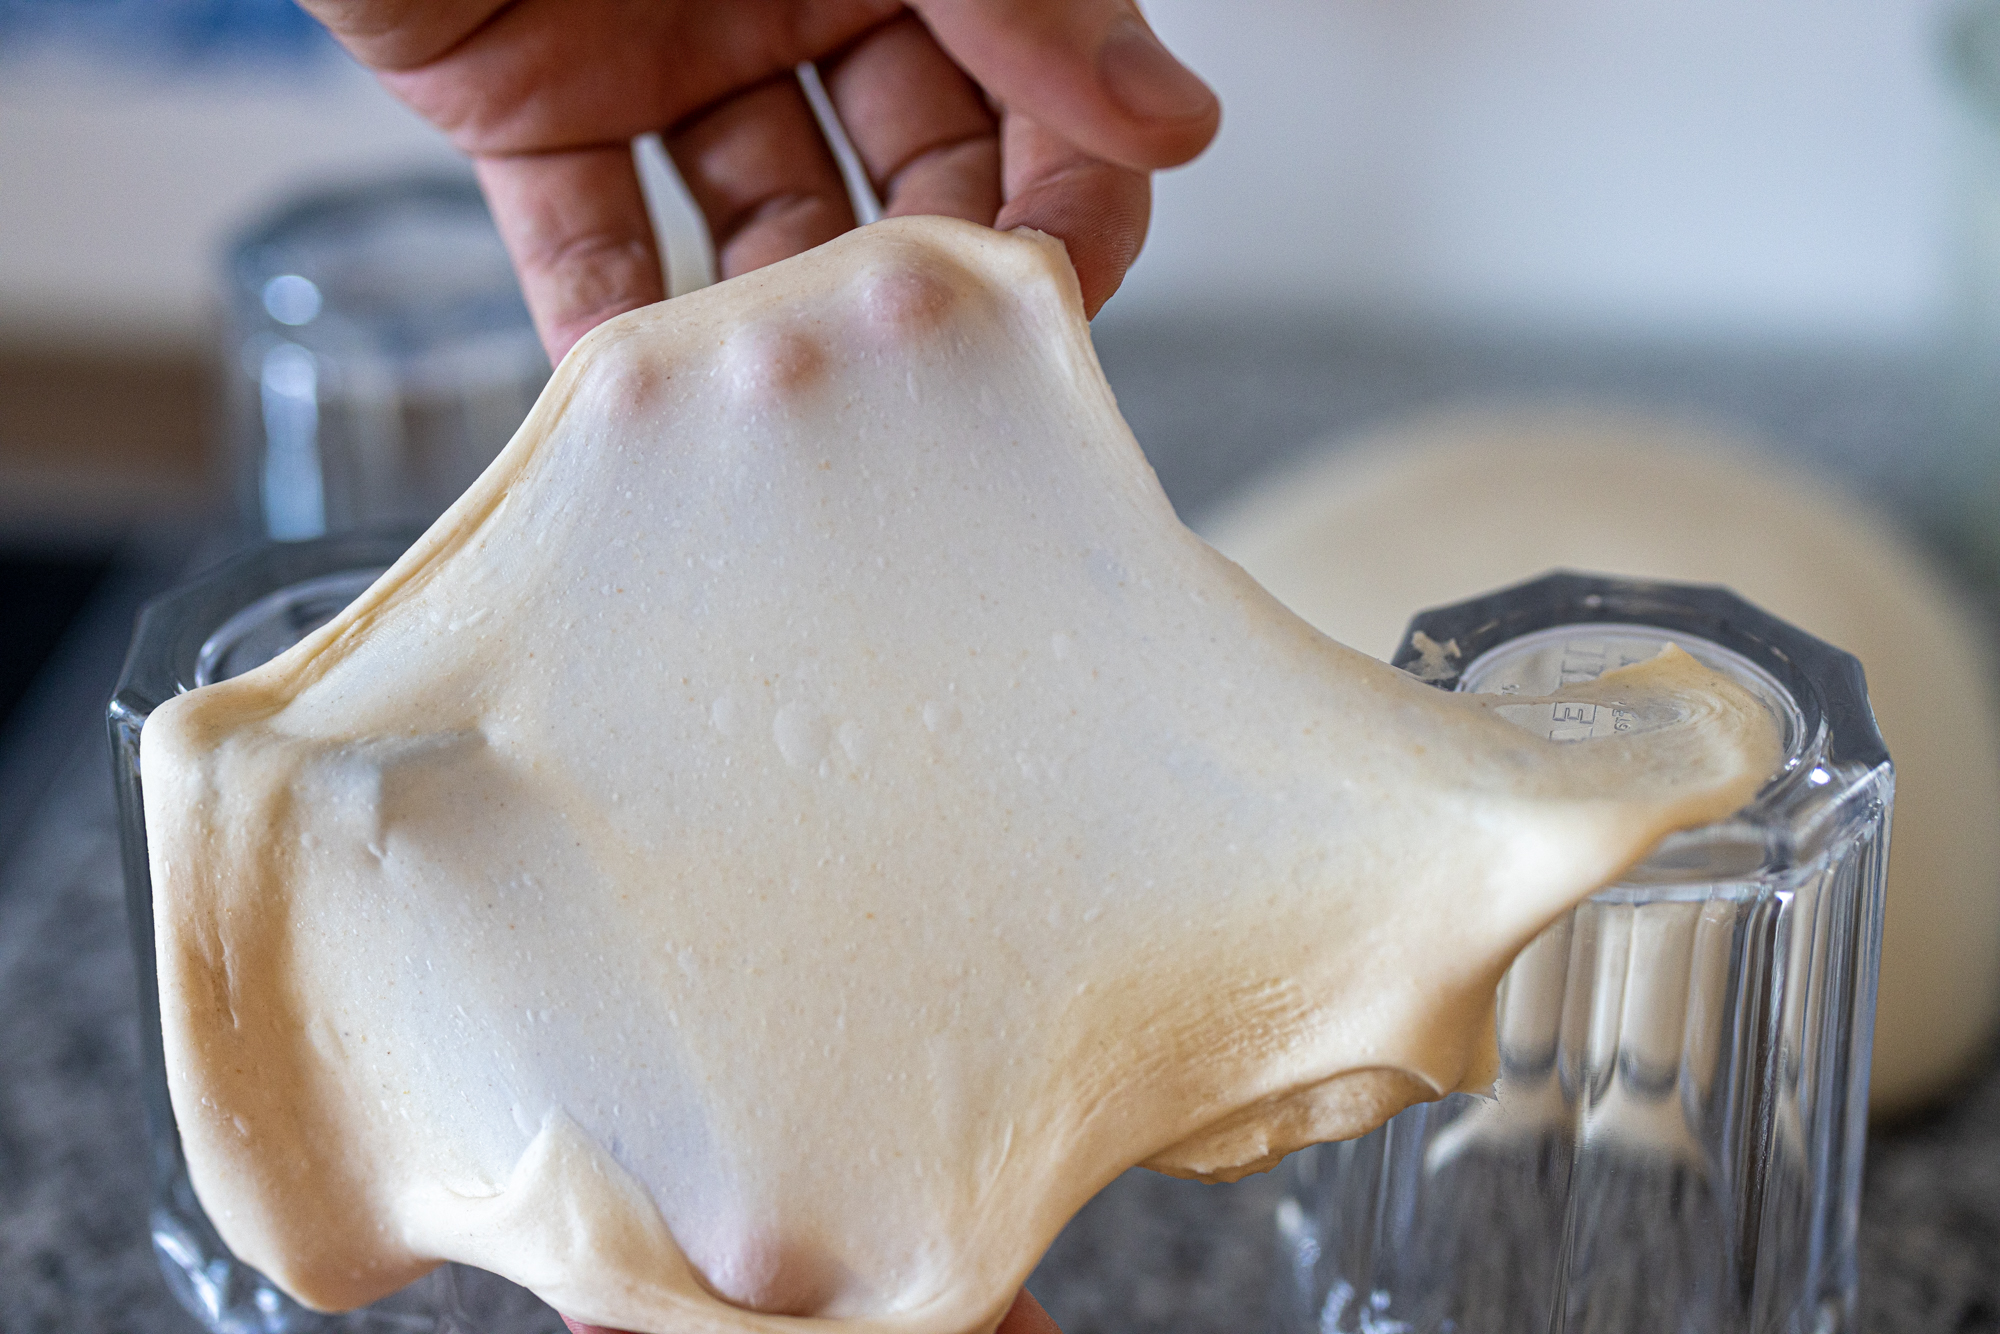
\includegraphics[width=\textwidth]{window-pane-effect}
  \caption[The window pane test]{The window pane test allows you to see if you
      developed your gluten well enough.}
\end{figure}


From an economic perspective, water is the cheapest component in your bread
dough. When running a bakery, a higher hydrated dough will weigh more and have
lower production costs. The profit will be higher. This comes at the price
of increasing labor costs and more potential failures due to the enhanced
difficulty.

\section{How much starter?}

Most bakers use around \qty{20}{\percent} sourdough starter based on the
flour weight.  I~recommend going much lower, to around
\qtyrange{5}{10}{\percent}.

By adjusting the amount of pre-ferment you can influence the time your dough
requires in the bulk fermentation stage. The more starter you use, the faster
this process is. The smaller the starter quantity, the slower. With a higher
quantity of starter, you are introducing more microorganisms to your main
dough. The higher this quantity, the faster the rate of fermentation in your
dough is.

The other factor influencing the rate of fermentation is the temperature of
your dough. The warmer the temperature, the faster the process; the colder, the
slower the process.

While food is available, the microorganisms will reproduce and increase in
quantity. The process is self-limiting: it stops when there is no
more food available. This can be compared to wine making where
the yeast ultimately sporulates and dies as ethanol levels increase. The ethanol creates an
environment that makes it impossible for other
microorganisms to join the feast. The same thing happens with the acidity
created by the bacteria. The high acidity slows the fermentation process and
prevents new microorganisms from entering the system.

Initially, your starter's properties are carried over to the main dough. Then,
as time progresses, the microorganisms adapt to the new environment. If your
starter is very bacterial then your main dough's fermentation will also be. You
end up with a dough that is not as fluffy as it could be. It will taste quite
sour, too sour for most people.

If you were to use an extreme value of around \qty{90}{\percent} starter based on your flour, there
would be very little room for the microorganisms to adjust in the main dough.
If you were to just use \qty{1}{\percent}, your microorganisms can regrow into a
desirable balance in the dough. Furthermore, you need to consider that a high value
of starter means a high inoculation with already fermented flour. As
mentioned earlier, enzymes break down the dough. This means the higher this
value, the more broken-down fermented flour you have. A too-long fermentation
always results in a very sticky dough that cannot be handled. The more
starter you use, the faster you will get to this point. If you were to use a
very little amount of starter, your flour might have naturally broken down
before the fermentation has reached the desired stage. You can observe this
when using a small quantity of around \qty{1}{\percent} sourdough starter. The small
amount of added microorganisms will not be able to reproduce fast enough
before the protease has broken down your dough completely.

As explained earlier the key to making great bread is a slow but not too slow
fermentation. Enzymes require time to break down your dough. Taking all this
into consideration, I~try to aim for a fermentation time of around 8 to 12~hours. This seems to be
the sweet spot for most of the flours that I~have worked with. To achieve this,
I~use around \qty{5}{\percent} of sourdough starter in summer times
(temperatures around \qty{25}{\degreeCelsius} (\qty{77}{\degF}) in the
kitchen). In winter times I~opt for around \qty{10}{\percent} up to
\qty{20}{\percent} sourdough starter (kitchen temperature around
\qty{20}{\degreeCelsius} (\qty{68}{\degF})). This
allows me to use a sourdough starter that's not in perfect condition. As
explained earlier, your
bread dough is essentially a gigantic starter. The low inoculation rate allows
the starter to regrow inside your main dough into a desirable balance.
Furthermore, the enzymes have enough time to break down the flour. This also
allows me to skip the so-called autolysis step completely (more in the next section).
This greatly simplifies the whole process.

\section{Autolysis}%
\label{section:autolysis}

Autolysis describes the process of just mixing flour and water and letting
this sit for a period of around 30~minutes up to several hours. After this
process is completed, the sourdough starter and salt are added to the
dough\footnote{I~have tested adding the salt at the start and end of the
autolysis process and could not notice a difference. Based on my current
understanding, the importance of adding salt later seems to be a myth.}.

The overall time that flour and water are in contact is extended. Thus you get the
beneficial enzymatic reactions that improve the taste and characteristics of the
dough. I~do not recommend autolysis as it adds an unnecessary step to the
process. Instead, I~recommend the fermentolysis technique which will be covered in the
next section of this book.

The effects of autolysis are very interesting. Try to mix just flour and
water and let that sit for a day. During the day, check the consistency of
your dough. Try and stretch the dough. If you dare, you can also taste the
dough throughout the day. With each hour, your dough will become
more extensible. It will be easier to stretch the dough. At the same time, your
dough will start to taste sweeter and sweeter. The protease and amylase enzymes
are doing their job. The same process is used when making oat milk. By letting
the mixture sit for some time, enzymes work on the oats. The taste is perceived as
sweeter and more appreciated. This process is further accelerated the more
whole-grain your flour is. The hull contains more enzymes. The gluten network
will ultimately tear, and your dough flattens out. For wheat sourdough, this is
your worst enemy. When this happens, your dough will become leaky and release
all that precious gas created during the fermentation. You need to find the
right balance of your dough breaking down just enough and not too much.

When you use a high inoculation rate of around \qty{20}{\percent} sourdough starter
your fermentation can be very quick. At \qty{25}{\degreeCelsius} it could be finished in as little as 5~hours.
If you ferment longer, your dough becomes leaky. At the same time, in
these 5~hours, the enzymes have not broken down the flour enough. This means
the dough might not be as elastic as it should be. Furthermore, not enough
sugars have been released and thus the flavor after baking is not good
enough\footnote{I~have not seen studies yet looking at enzymatic speeds depending on
the temperature. But I~assume the higher the temperature, the faster these
reactions. This goes up until a point when the enzymes break down under
heat.}. That's why bakers opt for autolysis. The autolysis starts the enzymatic
reactions before the microorganism fermentation begins. This way after 2~hours
of autolysis (an example) and 5~hours of fermentation the dough is in the
perfect state before beginning proofing.

When you try to mix your salt and starter into the flour/water dough you will
notice how cumbersome this is. It feels like you have to knead again from scratch
one more time. You will spend more time mixing dough.

For that reason, I~am strongly advocating utilizing the fermentolysis approach
which greatly simplifies the mixing and kneading process.

\section{Fermentolysis}%
\label{section:fermentolysis}

The fermentolysis creates the same advantageous dough properties the
autolysis creates without the headache of mixing your dough twice. You do this
by extending the fermentation time of your dough. Rather than doing a 2-hour
autolysis and 5-hour bulk fermentation you opt for an overall 7-hour
fermentation period.

To do this, you use less sourdough starter. A conventional recipe including the
autolysis step might call for \qty{20}{\percent} sourdough starter. Simply reduce this
value to \qtyrange{5}{10}{\percent}. The other option could be to place the dough in a colder
environment and thus reduce the speed at which your microorganisms replicate.

\begin{table}[!htb]
    \centering
        \documentclass[tikz]{standalone}
\usepackage{tikz}
\usepackage{siunitx}
\DeclareSIUnit\degF{\text{°}F}

\begin{document}
\begin{tabular}{|l|l|l|l|}
\hline
\textbf{\begin{tabular}[c]{@{}l@{}}Temperature\\ in °C\end{tabular}} & \textbf{\begin{tabular}[c]{@{}l@{}}Temperature\\ in °F\end{tabular}} & \textbf{\begin{tabular}[c]{@{}l@{}}Starter\\ recently fed?\end{tabular}} & \textbf{\begin{tabular}[c]{@{}l@{}}Amount\\ of starter in\%\end{tabular}} \\ \hline
30                                                                   & 86                                                                   & Yes                                                                      & 5                                                                         \\ \hline
25                                                                   & 77                                                                   & Yes                                                                      & 10                                                                        \\ \hline
20                                                                   & 68                                                                   & Yes                                                                      & 15                                                                        \\ \hline
30                                                                   & 86                                                                   & No                                                                       & 2.5                                                                       \\ \hline
25                                                                   & 77                                                                   & No                                                                       & 5                                                                         \\ \hline
20                                                                   & 68                                                                   & No                                                                       & 10                                                                        \\ \hline
\end{tabular}
\end{document}

        \caption[Quantity of sourdough]{A table visualizing how much sourdough
            starter to use depending on temperature and the starter's activity
            level.}
\end{table}

Based on my experience and my sourdough, my ideal bread always takes around 8
to 12~hours during bulk fermentation. Based on my availability throughout
the day, I~use a higher or lower starter quantity. If I~wanted to achieve a completed
fermentation in 8~hours, I~would opt for a \qty{10}{\percent} sourdough starter. If
I~wanted it to be ready in 12~hours, I~would opt for less starter, around \qty{5}{\percent}.
Simply mix all the ingredients and your fermentation begins. The
enzymes and microorganisms commence their work. On a very warm summer day, the
mentioned quantities no longer work. With a \qty{10}{\percent} starter, the same dough
would be ready in 5~hours up to a point of no return. Another additional hour
would cause the dough to break down too much. In this case, I~would opt for 5
percent sourdough starter to slow the whole process down to reach the 8 to 12
hour window again. If it is very hot, I~might use as little as \qty{1}{\percent}
sourdough starter\footnote{Please take these values with a grain of salt as
they depend on your flour and your sourdough starter. These are values that
you have to experiment with. After baking a couple of breads you will be able
to read your dough much better.}. You have to play with the timings on your own.
Rather than relying on timing though, I~will show you a much better and more precise approach
by using a fermentation sample. This will be covered later in this chapter.

Even for yeasted doughs, I~no longer use autolysis. I~just reduce the amount
of yeast that I~am using. Opting for the fermentolysis will
save you time and simplify your bread-making process. As mentioned in previous chapters,
the secret to making great bread is a slow but not too slow fermentation.

\section{Dough strength}

Dough strength is a fancy way to describe the bread-kneading process. As you wait and
knead, the gluten bonds in your dough become stronger. The dough
becomes more elastic and holds together better. This is the basis for trapping
all the gases during the fermentation process. Without the gluten network,
the gases would just diffuse out of your dough.

\begin{flowchart}[!htb]
\centering
  \begin{tikzpicture}[node distance = 3cm, auto]
  \node [start] (init) {\footnotesize Homogenize recipe ingredients};
  \node [block, right of=init, node distance=3cm] (wait1) {\footnotesize Wait 15~minutes};
  \path [line] (init) -- (wait1);
  \node [block, right of=wait1, node distance=3cm] (knead1) {\footnotesize Knead 5~minutes};
  \path [line] (wait1) -- (knead1);
  \node [block, right of=knead1, node distance=3cm] (wait2) {\footnotesize Wait 15~minutes};
  \path [line] (knead1) -- (wait2);
  \node [decision, below of=wait2, node distance=3cm] (windowpane_test) {\footnotesize Window-pane?};
  \path [line] (wait2) -- (windowpane_test);
  \path [line] (windowpane_test) -- node{no} (knead1);
  \node [decision, left of=windowpane_test, node distance=4.5cm] (more_water) {\footnotesize Bassinage for more water?};
  \path [line] (windowpane_test) -- node{yes} (more_water);
  \node [block, left of=more_water, node distance=4.5cm] (add_water) {\footnotesize Add water};
  \path [line] (more_water) -- node{yes} (add_water);
  \path [line] (add_water) -- (knead1);
  \node [block, below of=add_water, node distance=4cm] (wait3) {\footnotesize Wait 15~minutes};
  \path [line] (add_water) -- (wait3);
  \node [decision, right of=wait3, node distance=4.5cm] (dough_sample) {\footnotesize Aliquot sample?};
  \path [line] (wait3) -- (dough_sample);
  \path [line] (more_water) -- node{no} (dough_sample);
  \node [block, right of=dough_sample, node distance=4.5cm] (dough_ball) {\footnotesize Make round dough ball};
  \path [line] (dough_sample) -- node{no} (dough_ball);
  \node [block, below of=dough_sample, node distance=3cm] (extract_sample) {\footnotesize Extract sample};
  \path [line] (dough_sample) -- node{yes} (extract_sample);
  \path [line] (extract_sample) -- (dough_ball);
  \node [success, below of=dough_ball, node distance=3cm] (begin_bulk) {\footnotesize Begin bulk fermentation};
  \path [line] (dough_ball) -- (begin_bulk);
\end{tikzpicture}

  \caption{The gluten development process for a wheat-based dough.}%
  \label{fig:wheat-sourdough-kneading-process}
\end{flowchart}

It might sound odd, but the most important part of kneading is waiting. By
waiting you are allowing your flour to soak up water. This way the gluten
bonds of your dough form automatically and your dough becomes more elastic.
So you could be kneading for 10~minutes initially just to be surprised
that kneading 5~minutes and waiting 15~minutes has the same effect.

The gluten proteins glutenin and gliadin virtually instantly bond after being
hydrated. Disulfide bonds enable the longer portions of
glutenin to join with one another and form sturdy, extensible molecules.
Glutenins add strength, whilst the more compact gliadin proteins allow
the dough to flow like a fluid. Ultimately, the longer you wait, the more
your gluten network transforms into a web-like structure. This is what
traps the gases during the fermentation process~\cite{how+does+gluten+work}.

\begin{figure}[!htb]
  \centering
  \begin{tikzpicture}
    \tikzstyle{every node}+=[font=\normalsize\rmfamily]
    \begin{axis}[
        title style={align=center},
        title={Gluten development of a sourdough and yeast based dough\\
                \qty{22}{\degreeCelsius} (\qty{72}{\degF}) and
                \qty{60}{\percent}~hydration},
        axis x line=middle,
        axis y line=middle,
        width=\textwidth,
        height=0.5\textwidth,
        xmax=44, xmin=-0.1,
        ymax=12, ymin=-0.1,
        every axis y label/.style={%
            at={(ticklabel cs:0.5)},rotate=90,anchor=near ticklabel}, 
        every axis x label/.style={%
            at={(ticklabel cs:0.5)},anchor=near ticklabel}, 
        xtick distance=6,
        ytick style={draw=none},
        yticklabels={empty},
        legend style={draw=none},
        legend cell align={left},
        xlabel=Duration (hours), ylabel=Dough strength
        ]
        \addplot [color=redpic,smooth,ultra thick] table {plots/yeast.table};
        \addplot [color=codeblue,smooth,ultra thick] table {plots/sourdough.table};

        \node at (axis cs:18,7) [anchor=south west] {%
            \begin{tabular}{@{}lll@{}} \textbf{Dough type}&
            \textbf{Kneading} & \textbf{Stretch \& Fold}\\
            \midrule
            \textcolor{redpic}{Yeast}  & \textcolor{redpic}{None}&
            \textcolor{redpic}{None}  \\ \textcolor{codeblue}{Sourdough}&
            \textcolor{codeblue}{None} & \textcolor{codeblue}{None} \\
            \end{tabular}
        };
        \node at (axis cs:8,8.3) [anchor=south] {Peak stage};
        \node at (axis cs:1,1) [anchor=west] {Development stage};
        \node at (axis cs:9.5,5) [anchor=west] {Extensibility stage};
        \node at (axis cs:25.8,4) [anchor=west] {Decay stage};
    \end{axis}
\end{tikzpicture}

  \caption[Dough strength over time without kneading]{A schematic
      visualization of automatic gluten development. The doughs are not
      kneaded, just initially mixed.  Note how dough strength deteriorates
      over time as enzymes break down the flour. The effect is accelerated for
      sourdough due to the bacteria's gluten proteolysis.}%
  \label{fig:wheat-yeast-sourdough-degradation}
\end{figure}

The soaking process has to be extended the more whole-wheat flour is used.
The purpose of the wheat kernel's outer bran is to soak up water as fast
as possible. The enzymes become activated and start the sprouting process.
Because of this, less water is available for the gluten bonds to develop.
Either wait a bit longer or proceed and use slightly more water for
the dough.

This is the same principle that popular no-knead recipes follow. By making a less
hydrated dough and waiting your gluten network automatically forms. You still
have to mix and homogenize the ingredients. You wait a few minutes just to
find your dough having developed incredible dough strength with no additional
kneading\footnote{Give it a shot yourself. The automatic formation of gluten
networks is an amazing phenomenon that still fascinates me every time I~am
making dough.}.

If you over-hydrate your dough at the beginning it becomes more difficult
for the gluten chains to form. The molecules are not as close together in
a wetter dough compared to a stiffer dough. It is harder for the molecules
to align and form the web structure. For this reason, it is always easier
to start with lower hydration and then increase the water quantity if needed.
This is also commonly known as the \emph{Bassinage method}. The gluten
bonds have formed at the lower hydration and can then be made more extensible
by adding water and kneading again. This is a great trick to make
a more extensible dough with lower-gluten flour~\cite{bassinage+technique}.

When machine kneading a dough, opt for the same technique shown in
flowchart~\ref{fig:wheat-sourdough-kneading-process}.  Initially opt for a low
speed. This helps the homogenization process.
After waiting to allow the flour to soak up the water, proceed on a higher speed
setting. A good sign of a well-developed gluten network is
that your dough lets go of the container. This is because of the gluten's elasticity.
The elasticity is higher than the desire of the
dough to stick to the container.

\begin{figure}[!htb]
  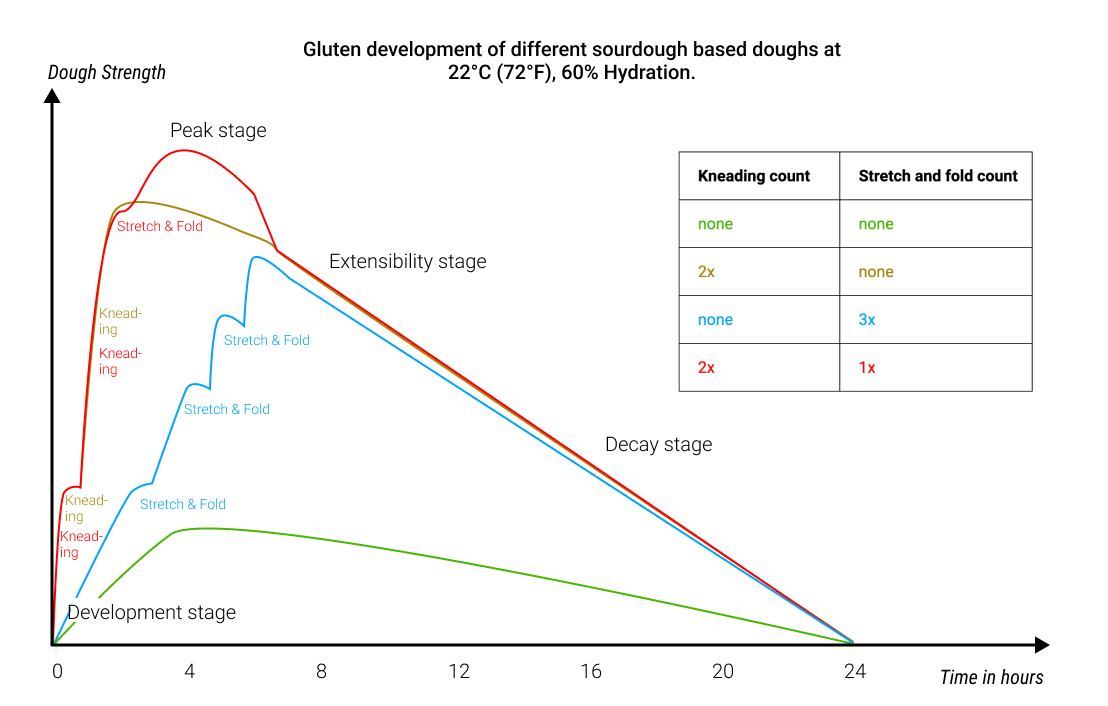
\includegraphics[width=\textwidth]{dough-strength-sourdough}
  \caption[Dough strength over time with kneading]{A schematic visualization
      of gluten development in sourdoughs with different kneading techniques.
      A combination of techniques can be utilized to achieve maximum dough
      strength.}%
  \label{fig:dough-strength-sourdough}
\end{figure}
% See https://www.figma.com/file/wTUVe6Nm2INOvT82mJhQur/Dough-strength-visualisation?node-id=0%3A1&t=fjdPvXYuJpsdQfWN-1 for
% the source of this visualization

Generally, the more dough strength you create, the less sticky your dough is going to
feel. As the dough holds together, it will no longer stick to your hands as
much. This is a common problem beginners face. Sticky dough is frequently
the sign of a not well enough developed gluten network.

\begin{figure}[!htb]
  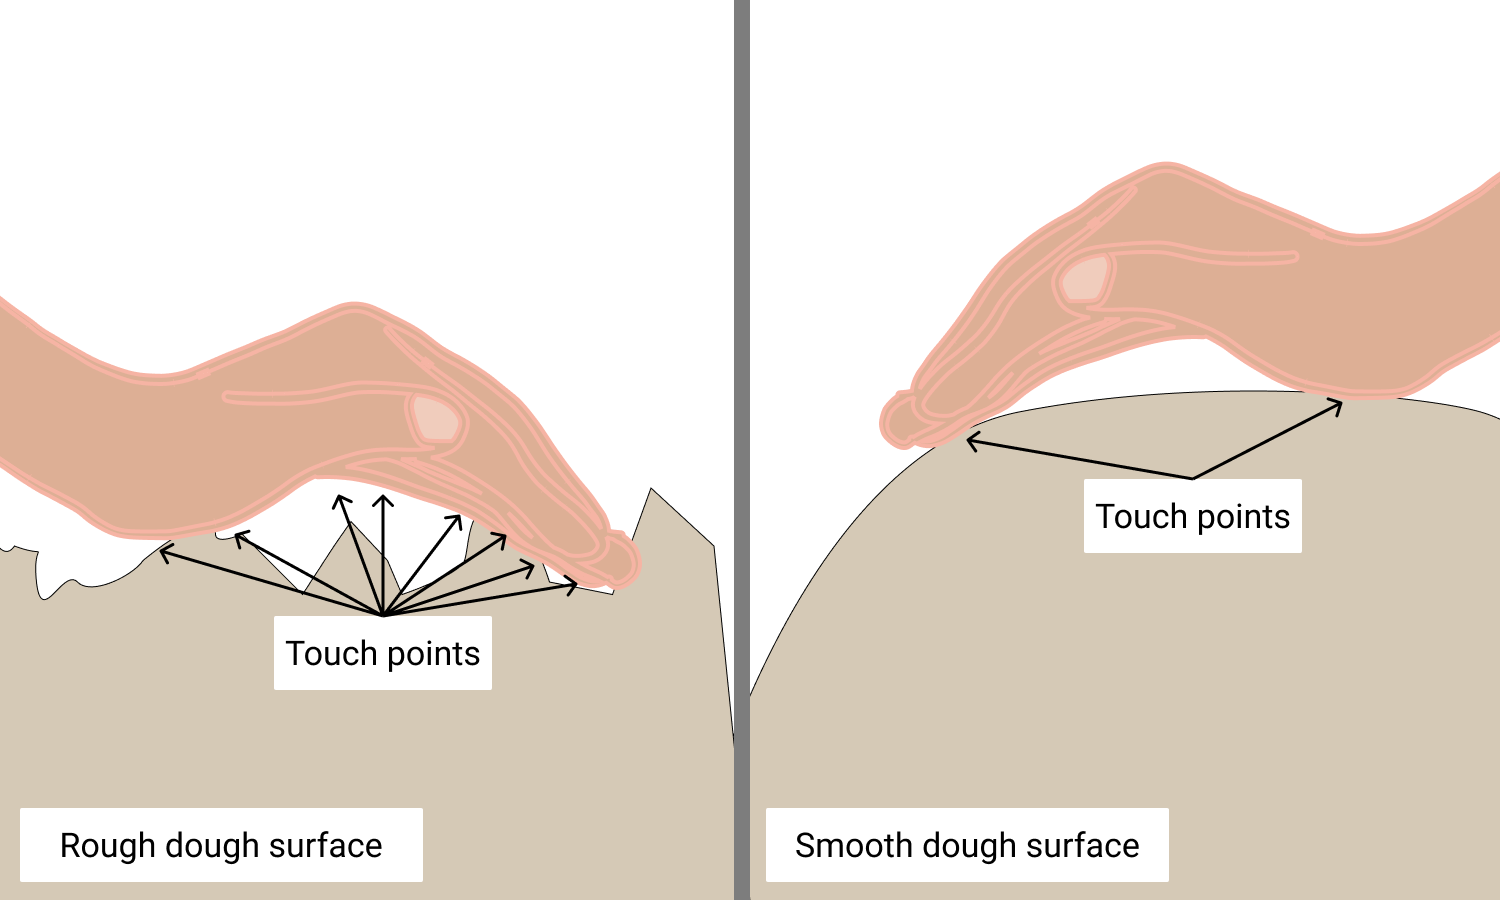
\includegraphics[width=\textwidth]{dough-surface-touchpoints}
  \caption[Touching the dough surface]{A schematic visualization of how a rough
      dough surface creates more touch points compared to a smooth dough
      surface.  By touching the rough surface the dough will swell and get into
      contact with more areas of your hand.}%
  \label{fig:dough-touch-points}
\end{figure}

Kneading more is generally beneficial in almost all cases, as it results in a
stronger gluten network. However, when making soft milk breads, you might prefer
a more extensible dough from the start. In this scenario, excessive kneading
could lead to a chewier final bread, which is not desirable if you aim for a
fluffier texture. Achieving this fluffier dough can be accomplished by kneading
less. While this is an exception, properly kneading your wheat-based doughs
is generally advised.

When you use a stand mixer, you can run into the issue of kneading too much. This
is almost impossible in practice though. Even after kneading for 30~minutes on medium
speed, my doughs hardly ever were over-kneaded. The moment you knead
too much, the color of the dough can begin to change. You mostly
notice this, though, during baking. The resulting loaf looks very
pale and white. This is because mixing dough causes oxidation,
which is necessary for the development of gluten.
However, if the dough is mixed too much, the compounds that contribute
to the bread's flavor, aroma, and color may be destroyed, negatively
affecting the quality of the bread~\cite{oxidization+dough}.

The last step before beginning bulk fermentation is to
create a smooth dough ball. By making sure your dough's surface is
smooth, you will have fewer touch points when touching the dough.
See figure~\ref{fig:dough-touch-points} for a schematic visualization
of how your hand touches a rugged and smooth dough.
With the smooth surface, your dough is going to stick less on your hands. Applying
later stretches and folds will be a lot easier. Without a smooth
surface, the dough becomes almost unworkable. Folding the dough later
becomes an impossible task. This is a frequent mistake I~see many
new bakers commit.

\begin{figure}[!htb]
  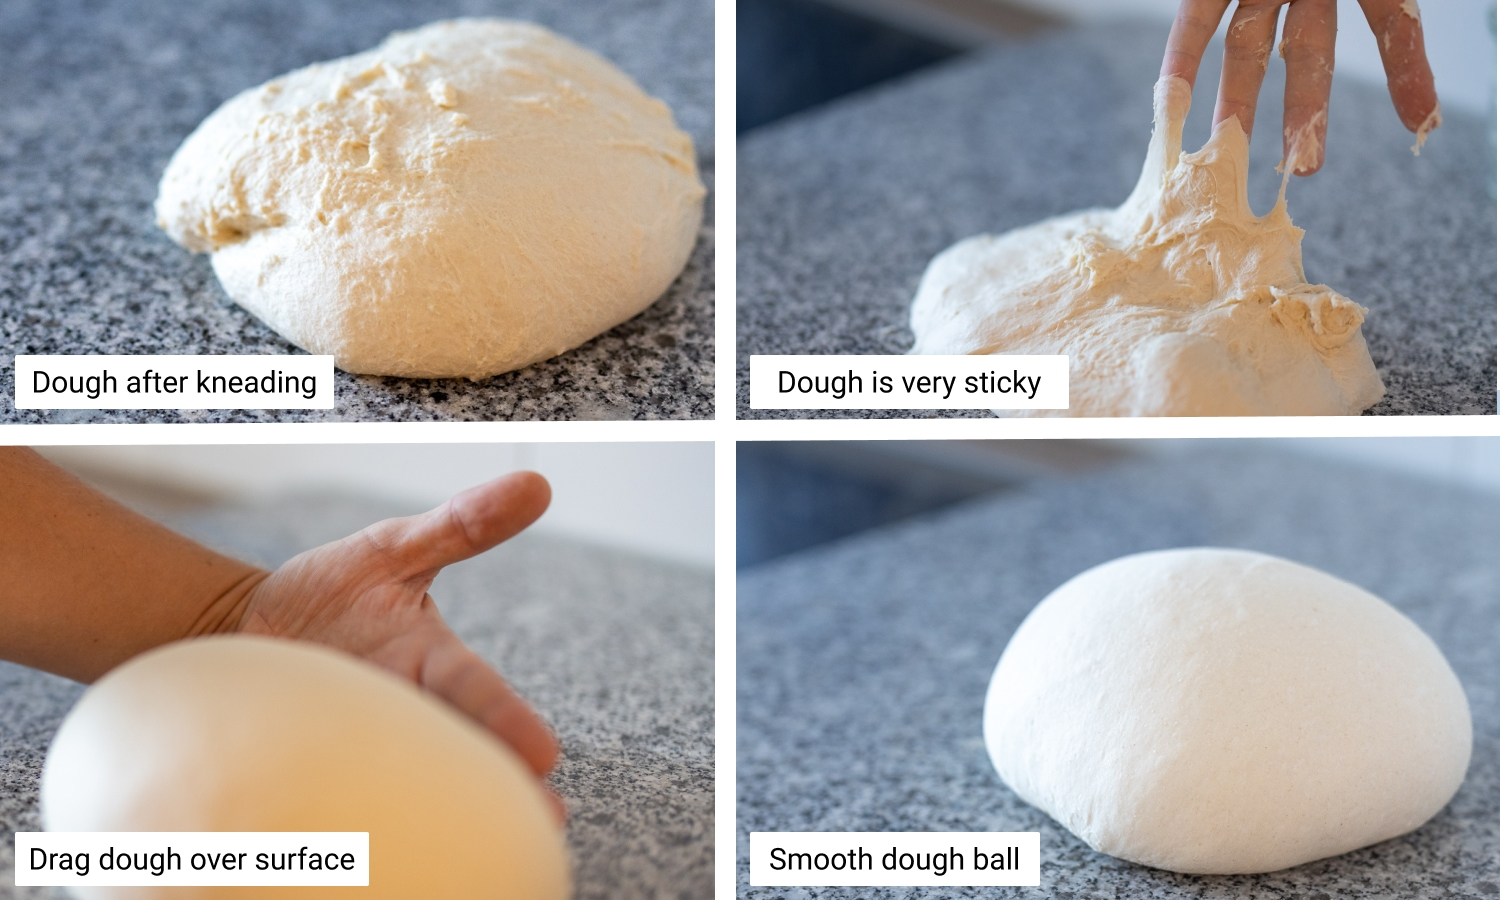
\includegraphics[width=\textwidth]{dough-ball-steps}
  \caption[Creating a smooth surface]{The transformation of a sticky dough
      blob to a dough with a smooth surface. The goal is to reduce surface
      touchpoints with your hands to make the dough less sticky when working
      it.}%
  \label{fig:dough-ball-steps}
\end{figure}

To make the dough's surface smooth, place your dough on a wooden board or
on your kitchen's countertop. Drag the dough with your palm over the surface.
A dough scraper could be used here for assistance.
Drag the dough towards you while making sure the top center of the dough stays in place.
It can help to gently place your second hand on top of the dough so that
the dough mass moves while retaining its orientation. Once the whole dough
is too close to the edge of the container/countertop, gently move it back
with two hands. By doing so, you are stretching the outer surrounding gluten layer.
For this reason, it is important to not use any flour during this process.
By using flour, you can no longer drag the dough over the surface and thus
you can't stretch the gluten. Always imagine you are touching something utterly sticky.
By doing so you will automatically try to touch the dough as little
as possible. Keep repeating the process until you see that the dough
has a nice smooth surface. The final dough should look like the dough
shown in~\ref{fig:dough-ball-steps}.

If your outer gluten layer tears, you have overstretched your dough. In
that case, take a 10-minute break, leaving your dough on the kitchen countertop.
This allows the gluten to re-bond and heal. Repeat the same process
and the damaged rugged areas should disappear.

The same dough-rounding technique is used later during
the pre-shaping process. After creating dough strength you
have all the time you need to practice rounding. Round the dough
as much as possible until it tears. Then wait the aforementioned 10~minutes and repeat.
Later, you don't have any room for error. Your technique has to be on point.
An over-pre-shaped dough can potentially not recover.

\section{Bulk fermentation}%
\label{section:bulk-fermentation}

After mixing the starter into your dough, the next stage of
the process known as bulk fermentation begins. The term
\emph{bulk} is used because in bakeries, multiple loaves are fermented
together in bulk. If you are a home baker, you might bulk
ferment a single loaf. The bulk fermentation ends when you
divide and pre-shape, or directly shape your final loaves or loaf.

The hardest part when making sourdough bread is controlling
the fermentation process. Bulking long enough but not too
long is the deciding factor for making great bread at home.
Even with poor shaping and baking techniques, you'll be able
to make excellent bread, solely by mastering the bulk
fermentation process.

With a too-short bulk, your crumb will be
perceived as gummy. Your crumb will feature large pockets of
air commonly referred to as \emph{craters}. A too-long fermentation
results in the dough breaking down too much. The resulting
dough will stick to your banneton and spread while baking
into a pancake-like structure.

The key is to find the sweet spot between not too little
and not too much bulk fermentation. I'd always recommend pushing
the dough more toward a longer fermentation. The
flavor of the resulting bread is better compared to a pale
underfermented dough.

\begin{table}[!htb]
    \centering
        \begin{tabular}{@{}>{\bfseries}p{0.12\textwidth}p{0.273\textwidth}p{0.273\textwidth}p{0.273\textwidth}@{}}
\toprule
 &\multicolumn{3}{c}{\textbf{Fermentation}}\\
 \cmidrule(rl){2-4}
 & \thead{Too short} & \thead{Too long} & \thead{Perfect} \\ \midrule
Crumb texture & Unbaked gummy areas towards the bottom of the bread.
              & Crumb can be perceived as gummy as most gluten broken down.
              & Crumb evenly baked. Crumb can be perceived as moist, but not gummy.
              \\ 
Alveoli       & Overly large alveoli in the crumb ``craters''.
              & Many tiny alveoli equally distributed.
              & Alveoli evenly distributed, no ``craters''.
              \\ 
Taste         & Pale neutral taste.
              & Strong acidic flavor profile. Acidity overweighs when tasting.
              & Balanced flavor profile, not too mild but also not too sour.
              Depending on starter vinegary or lactic notes.
              \\ 
Texture       & Overall poor texture.
              & Good consistency, crumb is not as fluffy as it could be.
              & Great combination of  textures.
              \\ 
Oven spring   & Vertical oven spring, mostly due to water evaporating and inflating the dough.
              & Very flat pancake like  structure after baking.
              & Great vertical oven spring. Dough grows more upwards rather than sideways.
              \\ \bottomrule
\end{tabular}

        \caption[Stages of sourdough fermentation]{The different stages of
            sourdough fermentation and the effects on crumb, alveoli, texture,
            and overall taste.}
\end{table}

The worst thing you can do when fermenting sourdough
is to rely on a recipe's timing suggestions. In \qty{99}{\percent}
of the cases, the timing will not work for you. The writer
of the recipe probably has different flour and a different
sourdough starter with different levels of activity. Furthermore,
the temperature of the fermentation environment might be
different. Just small changes in one parameter result
in a completely different timing schedule. One or two~hours'
difference results in the dough not fermenting long enough, or
turning it into a gigantic sticky fermented pancake. This
is one of the reasons why the current baking industry prefers
to make solely yeast-based doughs. By removing the bacteria
from the fermentation, the whole process becomes a lot more
predictable. The room for error (as shown in figure~\ref{fig:wheat-yeast-sourdough-degradation})
is much larger. The doughs are perfect to be made in a
machine.

\begin{flowchart}[!htb]
\centering
  \begin{tikzpicture}[node distance = 3cm, auto]
  \node [start] (init) {Bulk fermentation};
  \node [block, right of=init, node distance=4cm] (check_dough) {Check the dough};
  \node [block, right of=check_dough, node distance=4cm] (size_increase) {Check dough size increase};
  \node [block, below of=size_increase, node distance=2cm] (ph_value) {Check dough pH value};
  \node [block, below of=ph_value, node distance=2cm] (smell) {Check dough smell};
  \node [decision, right of=size_increase, node distance=4cm] (dough_ready) {Dough ready?};
  \node [success] at(dough_ready |- smell) (divide_preshape) {Divide and preshape};
  \node [decision, above of=size_increase] (dough_flattened) {Dough flattened out?};
  \node [block, above of=check_dough] (wait_60_minutes) {Wait\\ 60~minutes};
  \node [block, above of=wait_60_minutes] (stretch_fold) {Stretch and fold};

  \path [line] (init) -- (check_dough);
  \path [line] (check_dough) -- (size_increase);
  % Tricks not to get double lines
  \path [line] (check_dough) ++(2, -2) -- node{or} (ph_value);
  \path [line] (check_dough) ++(2, 0) -- node{} ++(0, -4) -- node{or} (smell);
  \path [line] (check_dough) ++(2, -4) -- node{or} (smell);
  \path [line] (size_increase) -- (dough_ready);
  % Same tricks not to get double lines and also we do _not_ want arrows
  \path [draw, thick] (ph_value) -- node{} ++(2, 0);
  \path [draw, thick] (smell) -| node{} ++(2, 4);
  \path [line] (dough_ready) -- node{Yes} (divide_preshape);
  \path [line] (dough_ready) |- node[right=3pt]{no} (dough_flattened);
  \path [line] (dough_flattened) |- node[right=3pt]{yes} (stretch_fold);
  \path [line] (dough_flattened) -- node{No} (wait_60_minutes);
  \path [line] (stretch_fold) -- (wait_60_minutes);
  \path [line] (wait_60_minutes) -- (check_dough);
\end{tikzpicture}

  \caption[Process to check the bulk fermentation]{During the bulk
      fermentation, multiple doughs are fermented together in bulk.  A
      challenging aspect of homemade sourdough bread is to determine when this
      stage of fermentation is completed. This chart shows multiple available
      options to check on the bulk fermentation progress.}%
  \label{fig:bulk-fermentation}
\end{flowchart}

Experienced bakers will tell you to go by the look and feel of
the dough. While this works if you have made hundreds of loaves,
this is not an option for an inexperienced baker. As
you make more and more dough, you will be able to judge
the dough's state by touching it.

My go-to method for beginners is to use an \emph{Aliquot jar}.
The aliquot is a sample that you extract from your dough. The
sample is extracted after creating the initial dough strength.
You monitor the aliquot's size increase to judge the
level of fermentation of your main dough. As your
dough ferments, so does the content of your aliquot jar. The moment your
sample reached a certain size, your main dough is ready
to be shaped and proofed. The size increase you should
aim for depends on the flour you have at hand. A flour
with a higher gluten content can be fermented for a
longer period. Generally, around \qty{80}{\percent}
of your wheat flour's protein is gluten. Check your flour's
packaging to see the protein percentage. The actual size increase
value is highly variable depending on your flour composition.
I~recommend beginning with a size increase of \qty{25}{\percent} and testing
up to \qty{100}{\percent} with subsequent bakes. Then identify a value
that you are happy with.

\begin{table}[!htb]
    \centering
        %TODO: Not great looking
\begin{tabular}{@{}cc@{}}
\toprule
\thead{Flour protein content} & \thead{Relative aliquot size increase} \\ \midrule
8--10\%              & 25\%  \\ 
10--12\%             & 50\%  \\ 
12--15\%             & 100\% \\ 
\textgreater{} 15\%  & \textgreater{} 100\% \\ \bottomrule
\end{tabular}

        \caption[Increase of size versus protein content]{Reference values for
            how much size increase to aim for with an aliquot jar depending on
            the dough's protein content.}
\end{table}

The beauty of the aliquot is that no matter the surrounding
temperature, you will always know when your dough is ready.
While the dough might be ready in 8~hours in summer, it could
easily be 12~hours in winter. You will always ferment your
dough exactly on point.


\begin{figure}[!htb]
  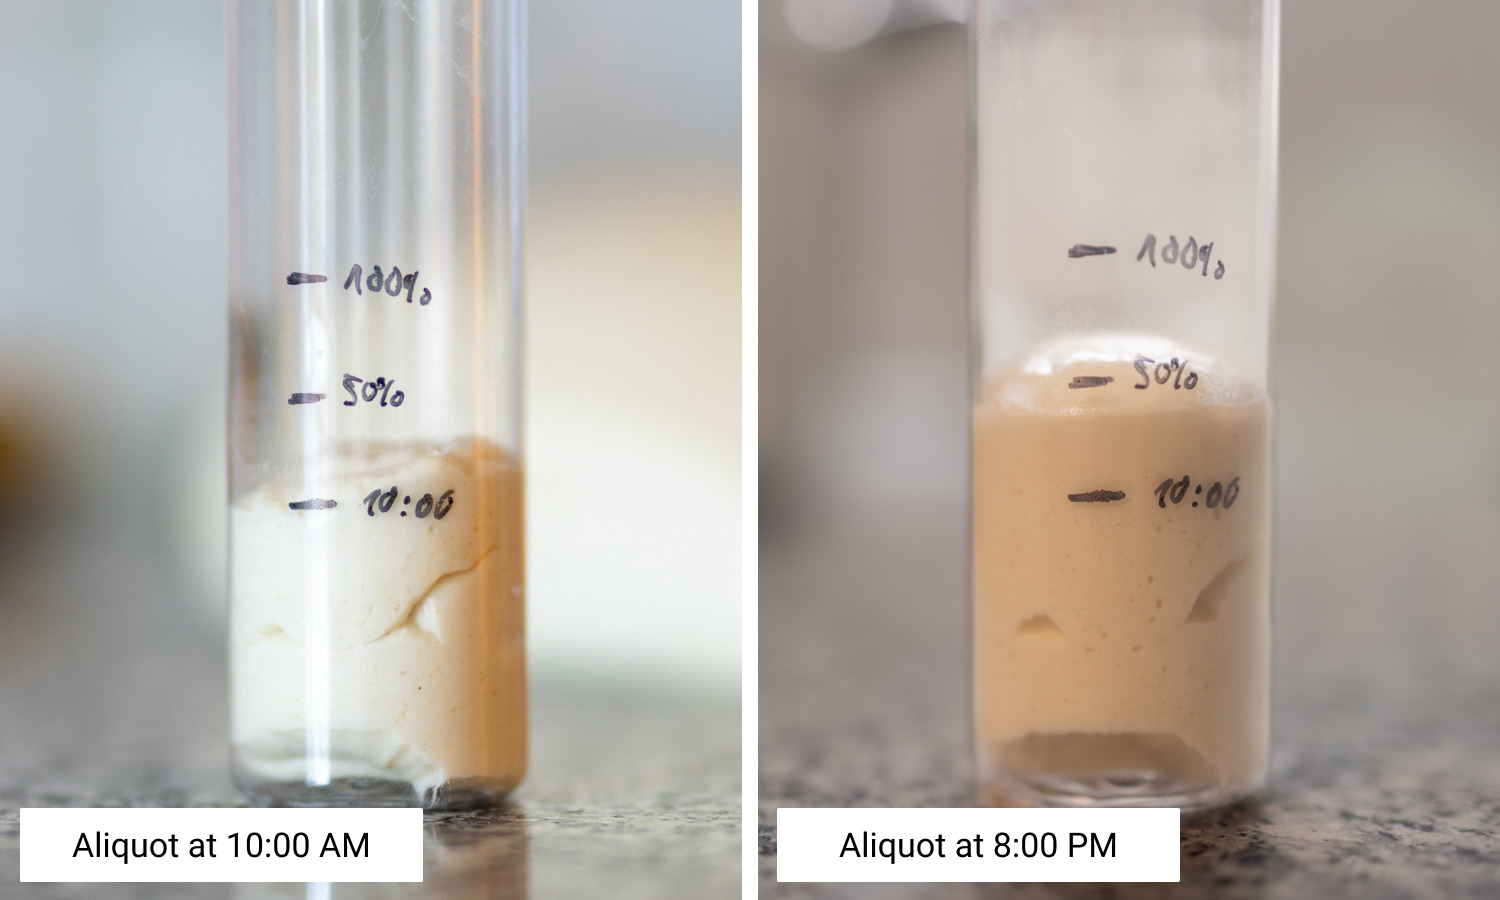
\includegraphics[width=\textwidth]{aliquot-before-after}
  \caption[Aliquot Jar]{An aliquot jar to monitor the dough's fermentation
      progress.  It took 10~hours for the dough to reach a \qty{50}{\percent}
      size increase.}
\end{figure}

While the aliquot sample has enabled me to consistently bake
great loaves, there are limitations to consider. It's crucial
to use a cylindrical-shaped container to properly judge
the dough's size increase. Furthermore, it is essential
to use room-temperature water when making your dough. If the
water is hotter, your aliquot, due to its smaller size,
will cool down faster. The aliquot will ferment more slowly
than your dough. Similarly, when you use too cold water,
your sample will heat up faster than the large dough mass.
In that case, your aliquot is ahead of your main dough. You
would probably stop the fermentation too early. Make sure
to keep the dough and aliquot close together. Some people even
place the aliquot in the same container. This makes sure that
both are in the same environment temperature. The aliquot
is also less reliable if your ambient temperature changes
a lot during the day. In that case, your aliquot will adapt
faster than your main dough. The readings will always be slightly
off. If you are making a large chunk of dough with more
than \qty{10}{\kg} of flour, the jar is also less reliable. The biochemical
reactions happening inside your dough will heat it.
The fermentation itself is exothermic which means
that it produces heat.

Another more expensive option is to use a pH meter
to monitor your dough's fermentation state. As the lactic
and acetic acid bacteria ferment, more acidity is piled
up inside your dough. The acidity value (pH) can be
measured using such a meter. The more acidity, the lower the pH
value of your dough. The pH scale is logarithmic, meaning
that each digit change will have a 10x increase in acidity.
A sourdough dough might begin fermenting at \pHvalue{6.0},
then shortly before baking has roughly \pHvalue{4.0}. This means
that the dough itself is 10x times 10x (= 100x) sourer
than at the beginning. By using the meter, you can always
judge the state of your dough's acidification and then act
accordingly.

To use the pH meter successfully, you need to find pH values
that work for your dough. Depending on your starter,
water, and flour composition, the pH values to look out
for are different. A stronger flour with more gluten
can be fermented for a longer period. To find out
the pH values for your bread I~recommend taking
several measurements while making your dough.

\begin{enumerate}
  \item Measure the pH value of your sourdough starter before using it
  \item Check the pH after mixing all the ingredients
  \item Check the pH before dividing and pre-shaping
  \item Check the pH before shaping
  \item Check the pH of your dough before and after proofing
  \item Check the pH of your bread after baking
\end{enumerate}

If the bread you made turned out successfully with your values,
you can use them as a reference for your next batch. If the
bread didn't turn out the way you like, either shorten
the fermentation or extend it a little bit.

\begin{table}[!htb]
    \centering
        \begin{tabular}{@{}lr@{}}
\toprule
\textbf{Step}       & {\textbf{pH Value}} \\ \midrule
Starter ready       & 4.20                \\ 
Mixing              & 6.00                \\ 
Dividing/preshaping & 4.10                \\ 
Shaping             & 4.05                \\ 
Before proofing     & 4.03                \\ 
After proofing      & 3.80                \\ 
After baking        & 3.90                \\ \bottomrule
\end{tabular}
%
        \caption[Dough's pH during bread preparation]{Example pH values for
            the different breakpoints of my own sourdough process.}%
        \label{table:sample-ph-values}
\end{table}

The beauty of this method is its reliability. Once you have found
out your good working values, you can reproduce
the same level of fermentation with each subsequent dough.
This is especially handy for large-scale bakeries that want
to achieve consistency in each bread.

While this method is very reliable, there are also certain
limitations to consider.

First of all the pH values that work for me likely won't work for
you. Depending on your own starter's composition of lactic
and acetic acid bacteria, your pH values will be different.
You can use the values shown in Table~\ref{table:sample-ph-values}
as rough ballpark figures. Regardless, you need to find values
that work for your setup.

Another limitation is the price. You will need to purchase
a high-tech pH meter, ideally, a meter featuring a spearhead
\footnote{Not every pH meter is suitable for measuring dough.
Please refer to the manual to make sure it is certified for
measuring the pH of liquid and semi-solid media. To receive
accurate pH readings further ensure that your pH meter
is properly calibrated.}.
This way you can directly poke the meter deep into the dough.
At the same time, automated temperature adjustments are a
feature to look out for. Depending on the temperature,
the pH value varies. There are tables you can use to
do the adjustment calculations. More expensive meters
have this feature built in. The pH meter loses accuracy
over time. For this reason, you need to frequently
calibrate it. The process is cumbersome and takes time.
Lastly, you need to carefully rinse the pH meter before
using it in your dough. The liquid surrounding the
head of your pH meter is not food-safe and thus should
not be eaten. I~rinse the meter for at least one minute
before using it to measure my dough's fermentation stage.

The last method to judge the state of bulk fermentation
is to read the signs of your dough. The more bread you have
made, the more accustomed you will become to this process.
Look out for the dough's size increase. This can sometimes
be a challenge when your dough is inside a container.
You can help yourself by marking your container. Some bakers
even use a transparent rectangular bulk container. You
can use a pen to mark the initial starting point. From there
on you can nicely observe the size increase. Similar to the
mentioned aliquot sample, look out for a size increase that works
for your sourdough composition.

\begin{figure}[!htb]
  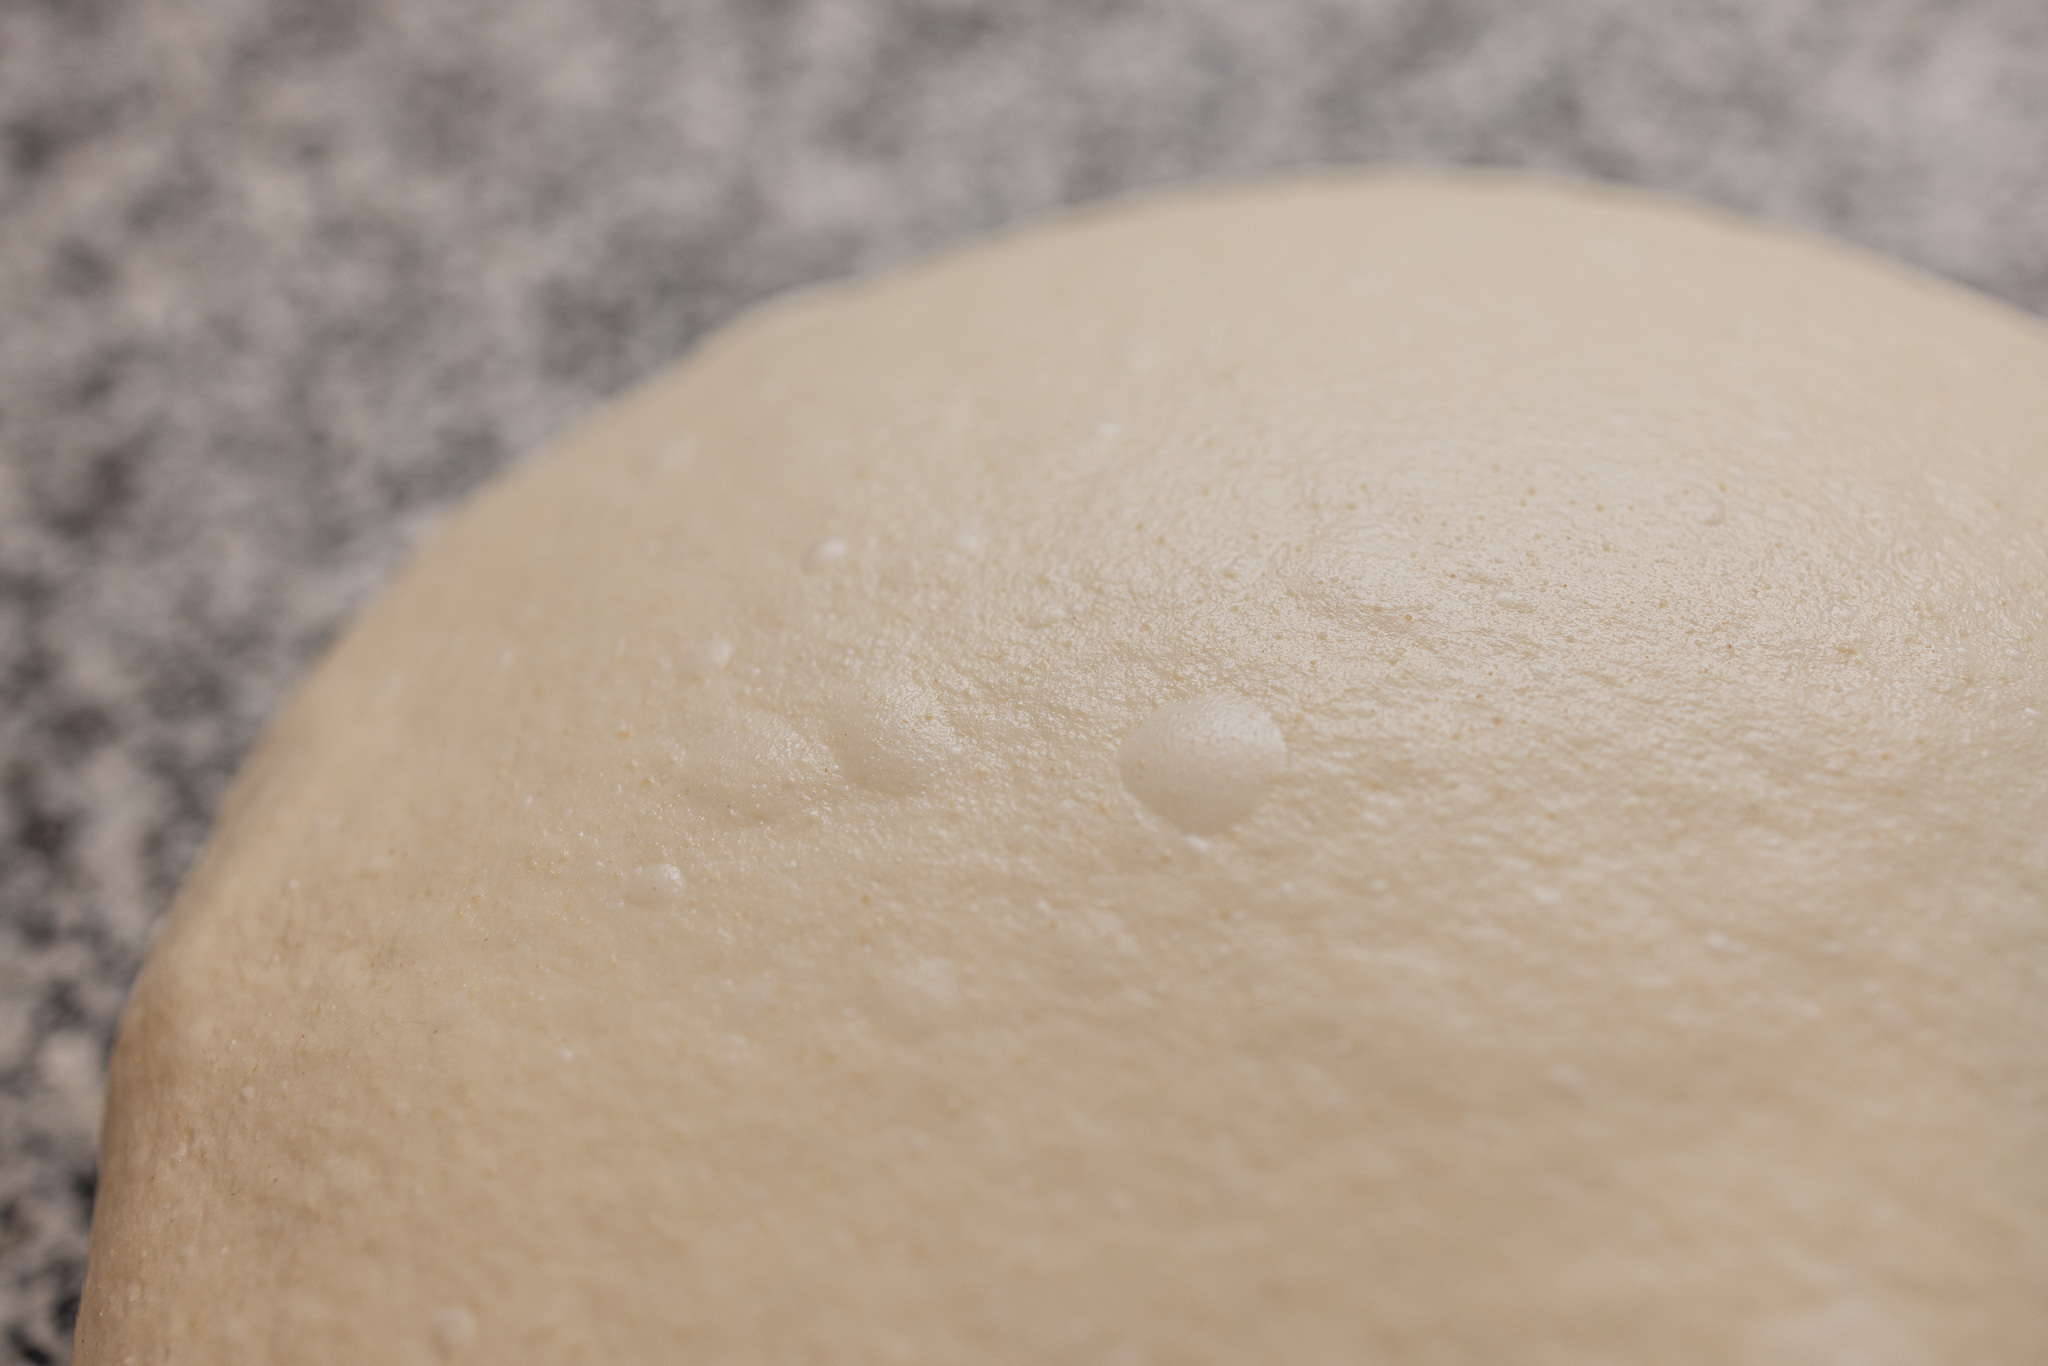
\includegraphics[width=\textwidth]{bulk-finished-dough}
  \caption[Dough at the end of bulk fermentation]{A dough in a good state to
      finish bulk fermentation. Notice the tiny bubbles on the dough's surface.
      They are a sign that the dough is inflated well enough.}
\end{figure}

Look out for bubbles on the surface of your dough. They
are a good sign that your dough is inflated with gas. The
further you push the bulk fermentation the more bubbles
will appear. If you overdo this stage, the dough becomes leaky, and
the bubbles will disappear again.

Take note of the dough's smell. It should match the same
smell of a ripe starter shortly before collapsing. As mentioned
before, your dough is nothing but a gigantic starter. You
can also proceed and taste your dough. It will taste like
pickled food. Depending on the acidity you can judge how
far the dough is in the fermentation process. The final bread
will taste less sour. That's because a lot of acidity evaporates
during baking\footnote{More on this topic later.
Just by baking longer and/or shorter, you can control
the tang of your final baked bread. The longer
you bake, the less sour the final loaf. The shorter,
the more acidity is still inside the bread. The resulting
loaf will be sourer.}.

When touching the dough, it should feel tacky
on your hands. The dough should also be less sticky
compared to earlier stages. If the dough is overly
sticky, you have pushed the fermentation too far.

If you pushed the bulk fermentation too far, you won't be able
to bake a freestanding loaf with the dough anymore. But don't
worry. You can move your dough into a loaf pan, or use parts
of the dough as the starter for your next dough. When using
a loaf pan, make sure it's properly greased. You might have
to use a spatula to transfer your dough. Allow the dough
to proof for at least 30~minutes in the loaf pan before
baking it. This makes sure that large cavities induced
by the transfer are evened out. You could push the proofing
stage to 24~hours or even 72~hours. The resulting
bread would feature an excellent, very tangy taste.


\section{Stretch and folds}

\begin{figure}[!htb]
  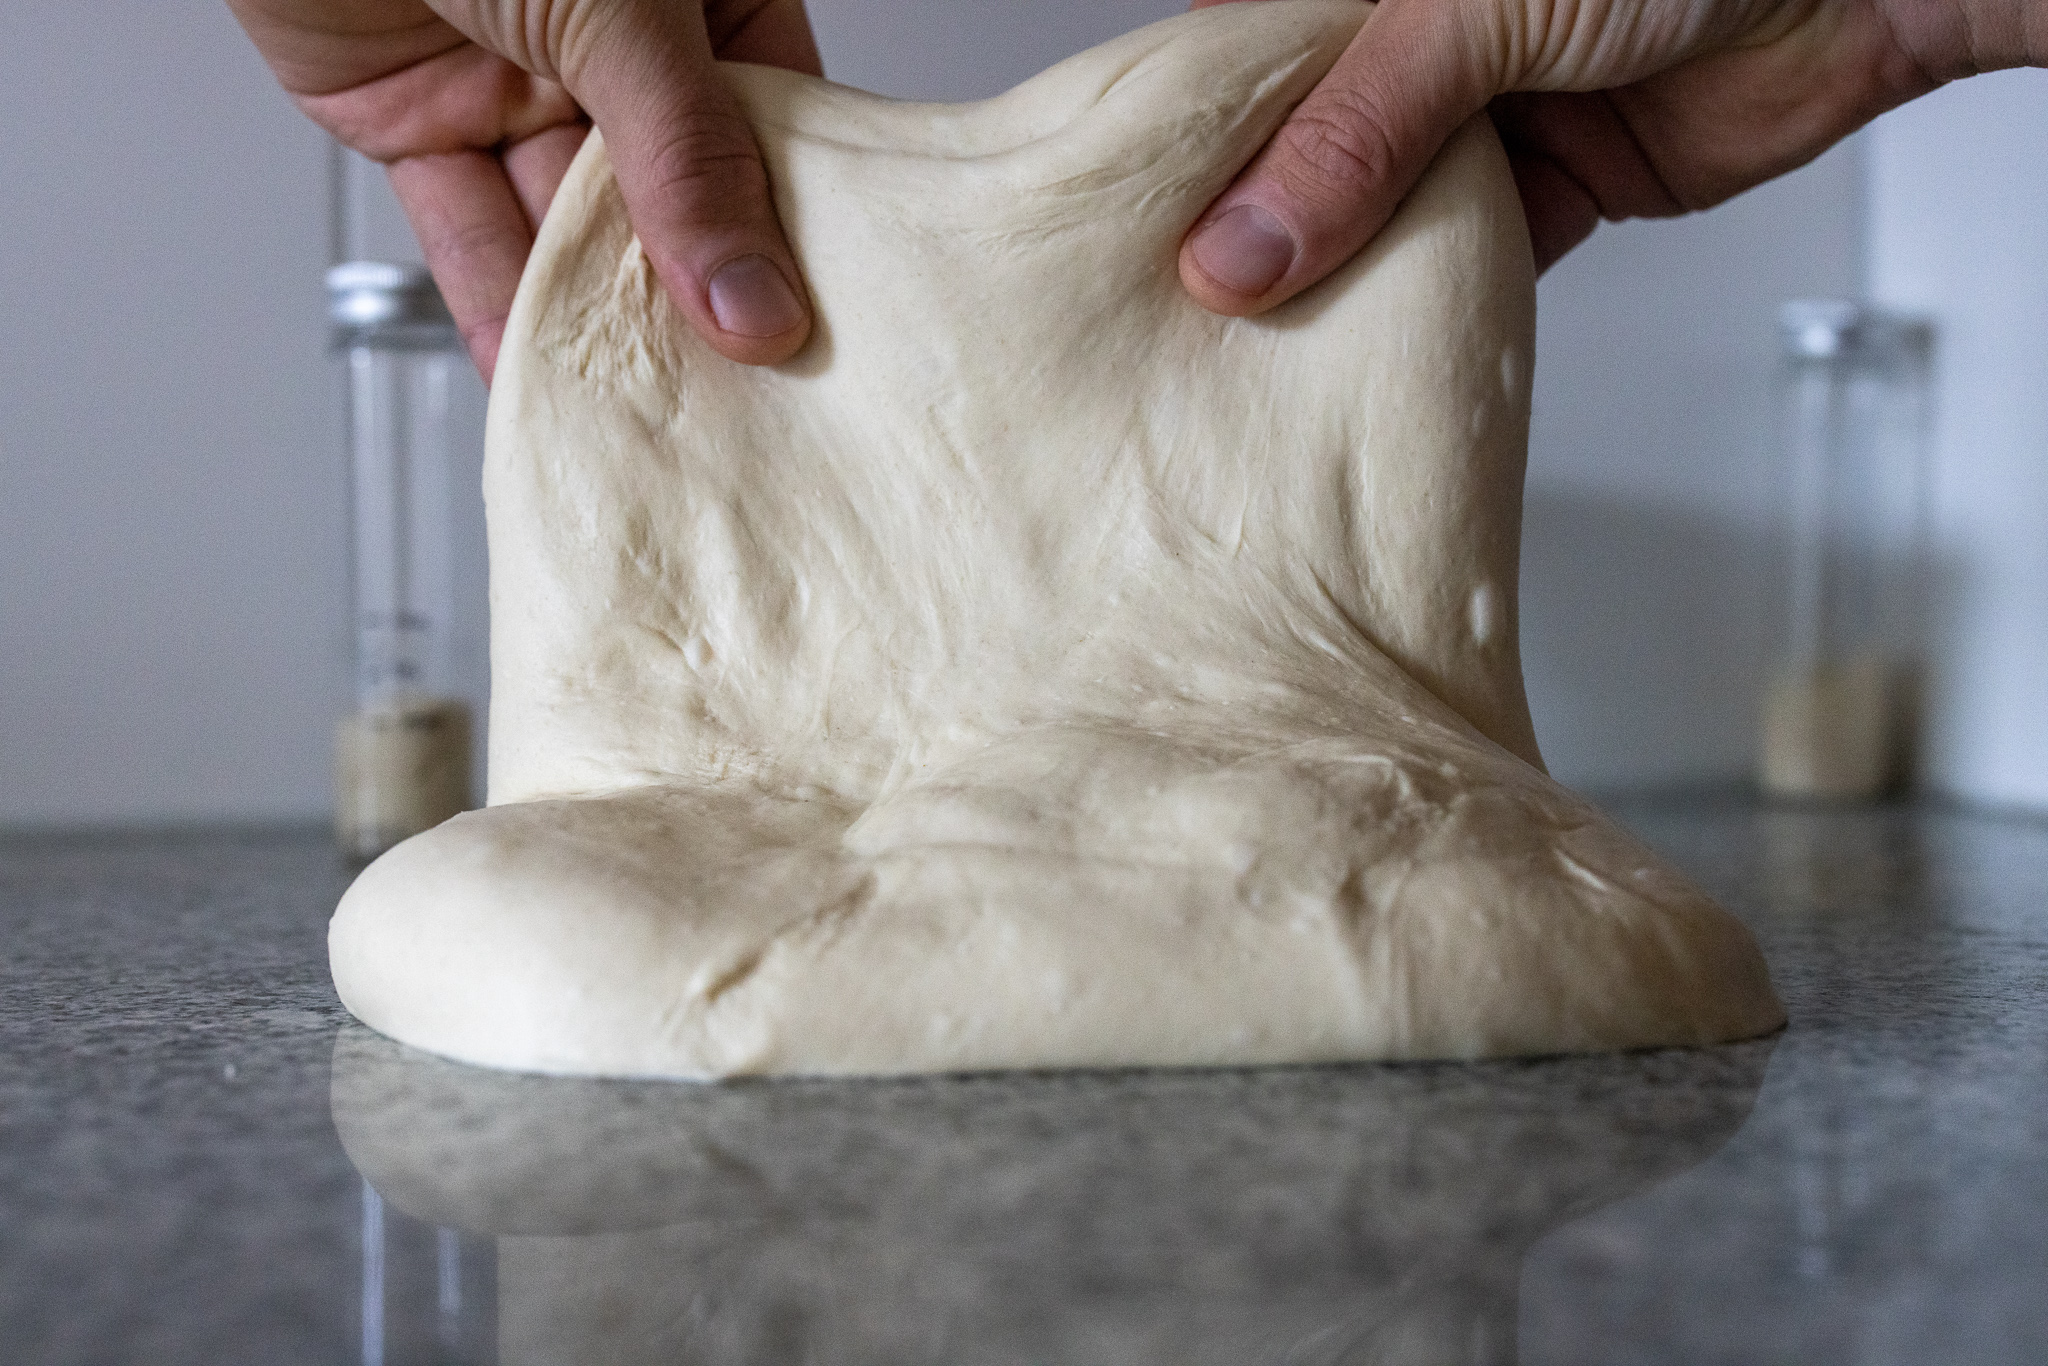
\includegraphics[width=\textwidth]{dough-being-glued}
  \caption[Gluing dough]{A dough where two sticky sides are being glued
      together using a stretch and fold. This process creates excellent dough
      strength.}
\end{figure}

In this section, you will learn all you need to know about stretching and
folding. You will learn when to stretch and fold and how to use this technique
to your advantage.

Stretching and folding is a set of techniques used by bakers during the bulk
fermentation stage. The process involves stretching the dough and then
folding the dough onto itself. Some recipes call for a single stretch
and fold, others for multiple.

The primary goal of this technique is to provide
additional dough strength to your dough. As shown in figure~\ref{fig:dough-strength-sourdough}
there are multiple ways to create dough strength\footnote{In fact I~have seen many no-knead
recipes calling for no initial kneading, but then applying stretch and folds
during the bulk fermentation. The time required to do all the folds probably
matches the initial kneading time required.}. If you do not knead as much at
the start, you can reach the same level of dough strength by applying stretch
and folds later. The more stretch and folds you do, the more dough strength
you add to your dough. The result will be a more aesthetic loaf that has
increased vertical oven spring.

Sometimes, if the dough is very extensible
and features very high hydration, stretching and folding is essential.
Without it, the dough itself would have too little dough strength and not
spring in the oven at all.

Another benefit of stretch and folds are their homogenization properties. By
folding the dough you are redistributing areas that are fermenting faster
than other areas. The heat in your dough is not the same in all areas.
The fermentation itself produces heat. For that reason, some of the areas in
your dough will ferment a little faster than others. This means that some
areas hold more gas and more acidity than others. Applying a stretch and fold
will redistribute heat, gas, and acidity. Some bakers also refer to this
process as crumb building. Careful folds ensure that your final dough's crumb
is not overly wild featuring large cavities. If you notice overly
large cavities in your final dough's crumb, then you might be able to fix that
by applying more stretch and folds\footnote{In many cases these cavities can
also happen when a dough does not ferment enough. The crumb is commonly called
Fool's Crumb. Refer to the later Debugging Crumb Structures chapter of this
book to learn more about it.}. Please refer to Section~\ref{section:debugging-crumb-structure}
``\nameref{section:debugging-crumb-structure}'' for more information on reading
your crumb.

\begin{figure}[!htb]
  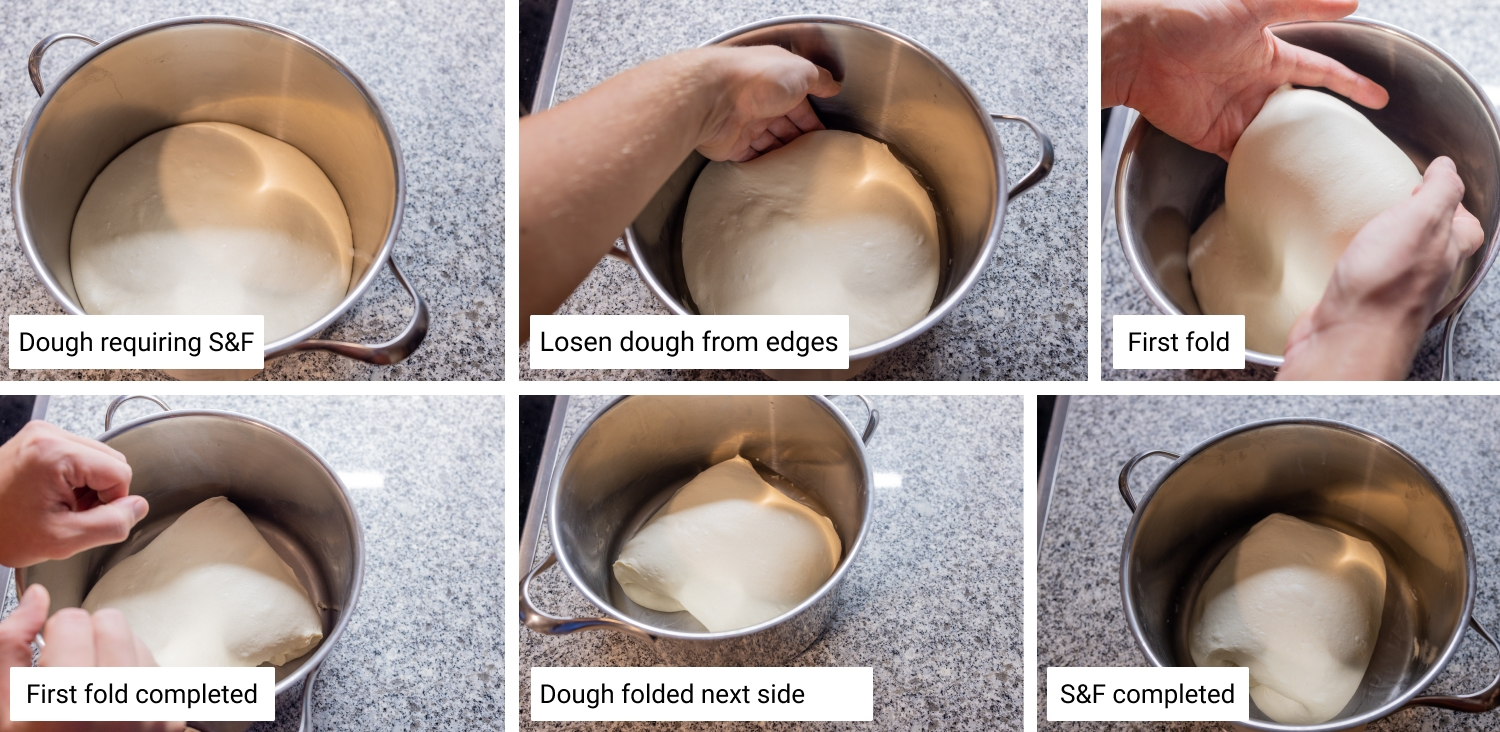
\includegraphics[width=\textwidth]{stretch-and-fold-steps}
  \caption[Stretch and fold steps]{An overview of the steps involved to perform
      stretch and folds for wheat-based doughs.}%
  \label{figure:stretch-and-fold-steps}
\end{figure}

The reason for the technique's popularity lies in its efficiency. By stretching
the dough outwards, you increase your dough's surface area. You then fold the
dough over, essentially gluing large areas of the dough together. Imagine a
piece of paper on which you place the glue. Then you fold the paper. Large areas
of the paper now stick together. Repeat the same process with more glue until
you have created multiple layers of paper and glue. This is the same thing that
happens to your dough. With only very few movements you have applied glue to your
dough.

To apply a stretch and fold first wet your hands with cold water. Watered hands
work wonders in reducing the dough's tendency to stick to your hands. Proceed and
carefully loosen the dough from the edges of your bulk container. Do this by
carefully placing your hand at the edge of the dough and pushing your hand
downwards on the container's walls. Once you have reached the bottom, drag the dough
a little bit inwards. The dough should stay in place and not move back to the
edge of your container. Try to be as swift as possible with this motion. The
slower you are, the more dough will stick to your hands. Repeat the same process
once all around your dough until the dough is free of your container's edges.
Wet your hands one more time and then carefully lift one side of the dough with
two hands placed in the center upwards. Make a fold in the center of the dough.
The upper smooth side needs to be placed on the bottom of the container. By doing
so, you will be gluing together the two sticky bottom sides. The top smooth side should
not be sticky in your hands, while the bottom rough surface should tend
to stick to your hands. Rotate the container
and repeat the same thing from the other side. Rotate the container 90°
and then repeat the process once again. Rotate the container another 180° in
the same direction
and repeat the fold one last time. By doing so you have applied 4 folds in total. Your
dough should now stay in place and resist flowing outwards\footnote{Please
also refer to~\cite{stretch+and+fold+technique} for a video showing you how to
best perform the technique.}.

In theory, there is no limit to how often you can stretch and fold. You could
apply one every 15~minutes. If your dough has enough dough strength already,
applying additional folds is just a waste of time\footnote{You could do it
just to better understand how the dough feels in your hands at different
fermentation stages.}. If you apply a large number of consecutive folds, the
outer layer of gluten
will tear. In that case, you just have to wait for at least 5--10~minutes until
the gluten bonds heal and you can try again. When the gluten does not heal
anymore, chances are you have pushed the fermentation for too long. Likely
most of the gluten has broken down and you are already
in the decay stage shown in figure~\ref{fig:dough-strength-sourdough}.

\begin{figure}[!htb]
  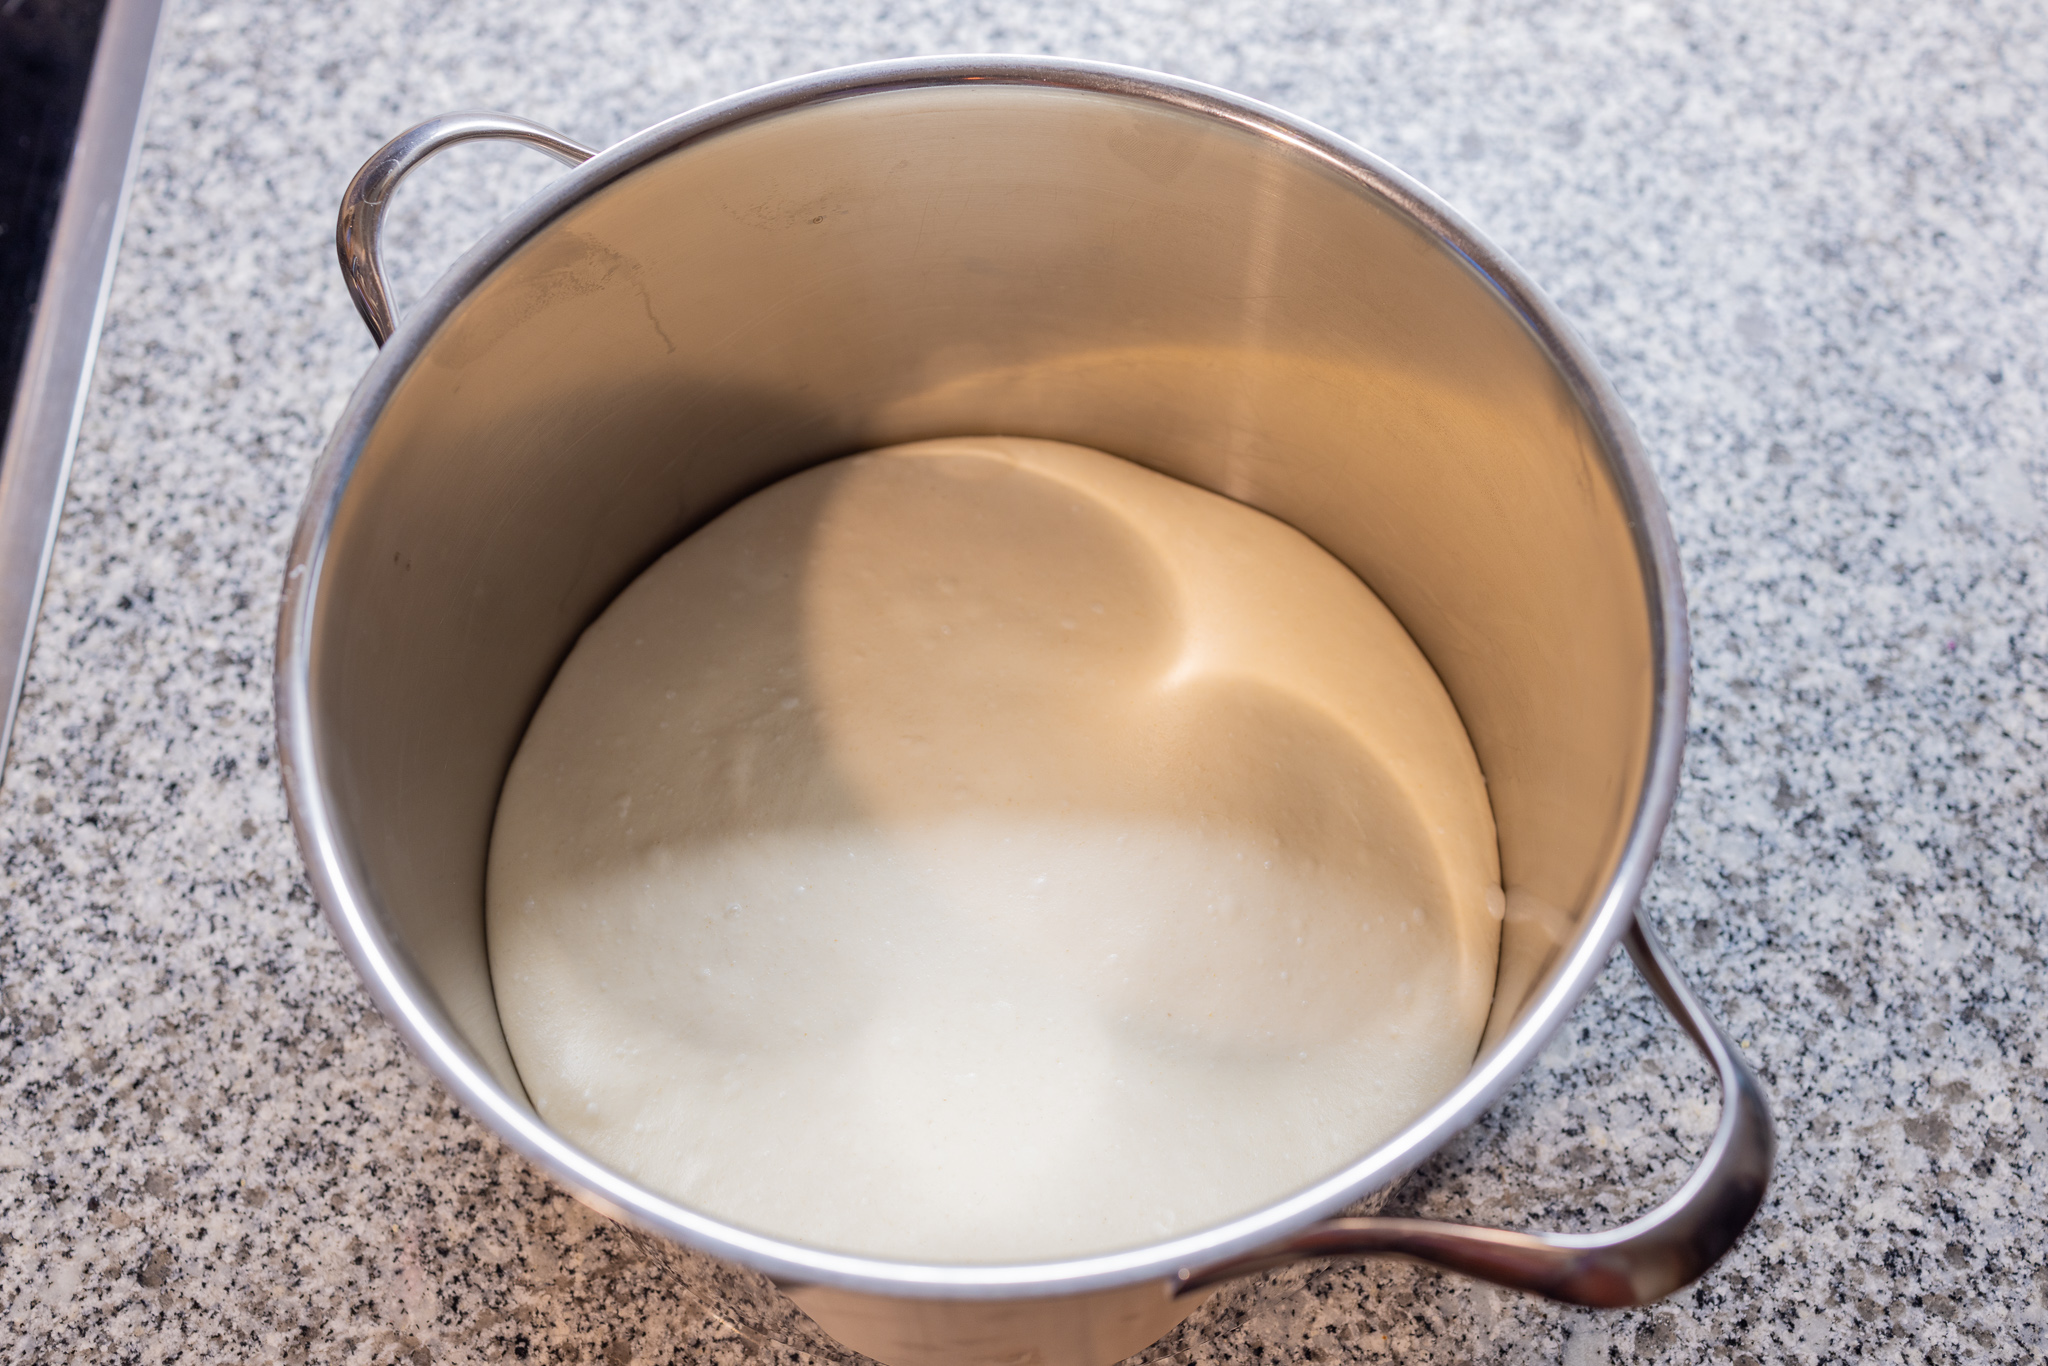
\includegraphics[width=\textwidth]{dough-requiring-stretch-and-fold}
  \caption[A flattened out dough]{A dough during bulk fermentation that has
      flattened out. To improve its dough strength, a stretch and fold should
      be applied.}
\end{figure}

Now, the reasonable amount of stretch and folds you should do greatly depends on how much you
kneaded initially and how extensible your dough is. A good recommendation is
to observe your dough in your bulk container. Once you see that the dough
flattens out quite a lot and spreads towards the edges of your bulk container,
you can proceed and apply a stretch and fold. For \qty{95}{\percent} of the doughs
that I~am making, this is hardly more than once. I~like to make overnight
doughs and in that case, I~typically apply one stretch and fold directly after
waking up. Then the bulk fermentation might take another 2~hours before I~proceed
with dividing and pre-shaping or directly shaping.

\section{Optional: Dividing and Preshaping}

Dividing and pre-shaping is an optional step that is done
once your sourdough finishes with the bulk fermentation stage.
The step is required if you are making multiple loaves in one
batch. It is optional if you are making a single loaf.

\begin{flowchart}[!htb]
\centering
  \begin{tikzpicture}[node distance = 3cm, auto]
  \node [start] (init) {\footnotesize Dividing required?};
  \node [decision, right of=init, node distance=5cm] (more_than_one_loaf) {\footnotesize More than 1 loaf?};
  \node [success, right of=more_than_one_loaf, node distance=5cm] (yes) {\footnotesize Yes};
  \node [success, below of=yes, node distance=3cm] (no) {\footnotesize No};
  \path [line] (init) -- (more_than_one_loaf);
  \path [line] (more_than_one_loaf) -- (yes);
  \path [line] (more_than_one_loaf) -- (no);
\end{tikzpicture}

  \caption[Is dividing your dough required check]{Dividing is only required when you are
      making multiple loaves in a single dough batch.}%
  \label{fig:dividing-decision-tree}
\end{flowchart}

The goal of dividing your dough into smaller pieces is to portion
your dough accordingly. This way you'll have multiple pieces of bread
which all weigh the same. For this reason, a scale is commonly
used to weigh the pieces of dough. If one piece of dough weighs
too little you can simply cut a bit more from your dough blob
to increase its weight.

When cutting the dough, try to be as concise as possible with your
movements. You don't want to unnecessarily damage your dough too much.
Quick movements with a knife or dough scraper help to prevent the
dough from sticking too much to your tools.

\begin{figure}[!htb]
  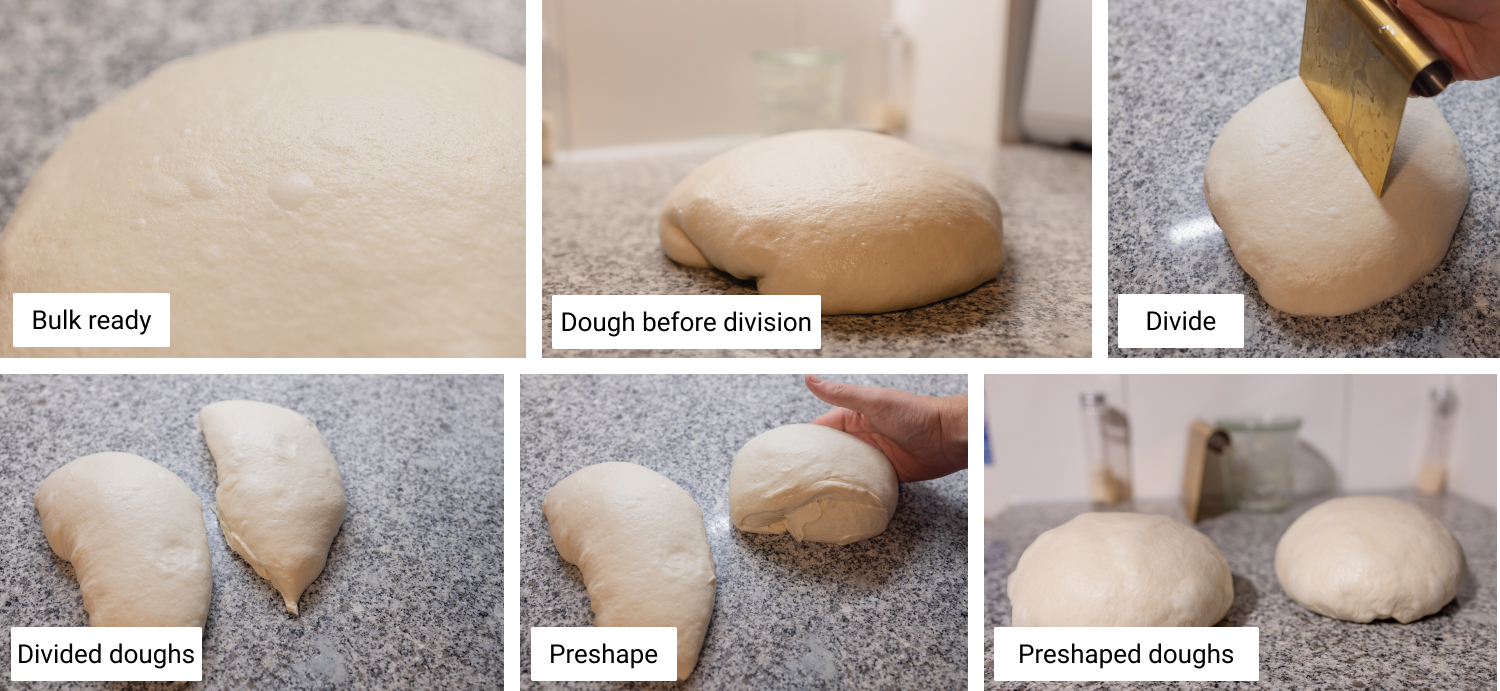
\includegraphics[width=\textwidth]{divide-preshape}
  \caption{The steps of dividing and preshaping your dough.}
\end{figure}

I~sometimes like to draw small lines with the dough scraper's edge
on the large dough mass before cutting it into smaller pieces.
This helps me to better plan where I~want to do my incisions. When
I~plan to make 8 loaves I~try to use the lines to divide the dough
into 8 equally sized portions before cutting. If this is not precise enough,
you can use the aforementioned scale.

Now that you have cut your dough, the resulting chunks are not in an equal shape.
This is problematic for the next stage when you are shaping your dough.
The resulting loaves wouldn't look nice and even. You would probably
end up with areas that tear the moment you are shaping your dough.
You wouldn't start the whole proofing process on a good foundation. For that
reason, you need to pre-shape your dough.

Pre-shaping is done for several reasons:
\begin{itemize}
  \item You divided your dough and require pre-shaping
  \item Your dough lacks dough strength. Pre-shaping will add more strength
  \item You want to even out the final loaf's crumb structure. By pre-shaping,
  the resulting crumb will look more even.
\end{itemize}

If you are making a single loaf from one dough batch the step is not required.
In that case, you can directly proceed with shaping, skipping this step.

The pre-shaping technique is the same as the process figure~\ref{fig:dough-ball-steps}.
Whereas earlier you could tear the dough's surface this could now result in a catastrophe.
For this reason, I~recommend practicing this step for as long as you need after kneading.
The gluten network might be so extensible and degraded at this point that there
is hardly any room for error. The dough wouldn't come together again. The only
way to save such dough is to use a loaf pan.

\begin{figure}[!htb]
  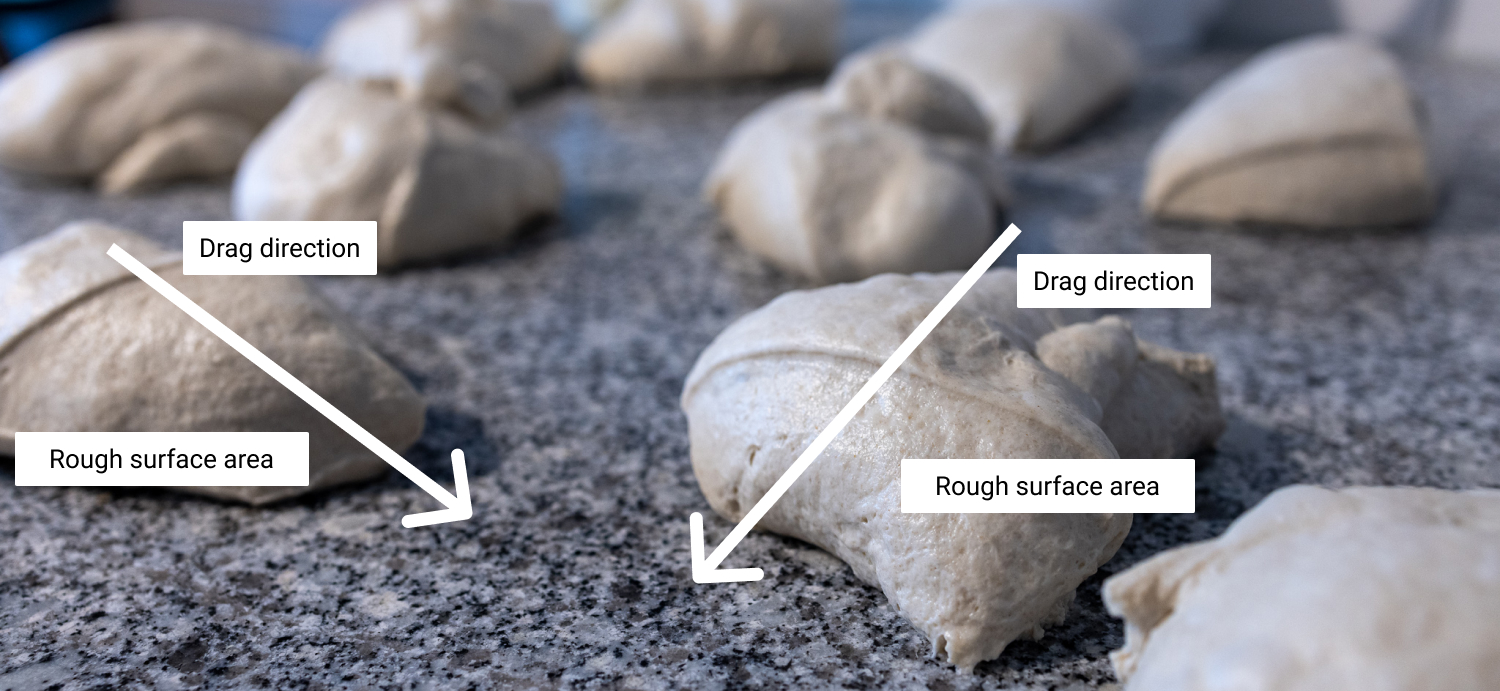
\includegraphics[width=\textwidth]{preshape-direction}
  \caption[Dragging direction]{Drag the dough in the direction of the rough
      surface area. This way you minimize the movements required to complete
      the step.}%
  \label{fig:preshape-direction}
\end{figure}

Pre-shape the dough as much as is needed to round up the top
surface area. Try to touch the dough as little as possible
to reduce its ability to stick to your hands. Drag the dough
in the direction where you see a rough surface area. In
case you have too little space to drag the dough because it might
fall from the edge of your counter, simply lift it with a swift movement and place
it in a better position for pre-shaping. Please refer to figure~\ref{fig:preshape-direction}
for a visualization showing the pre-shaping direction.

Try to set yourself a limit of movements to finish pre-shaping
a dough. Then you will be more conscious about each movement
you are performing. At the start you can try 5 movements,
iteratively reducing this to 3. The only reason for exceeding these
numbers could be if you on purpose want to even out the crumb
structure of your final loaves further.

\begin{figure}[!htb]
  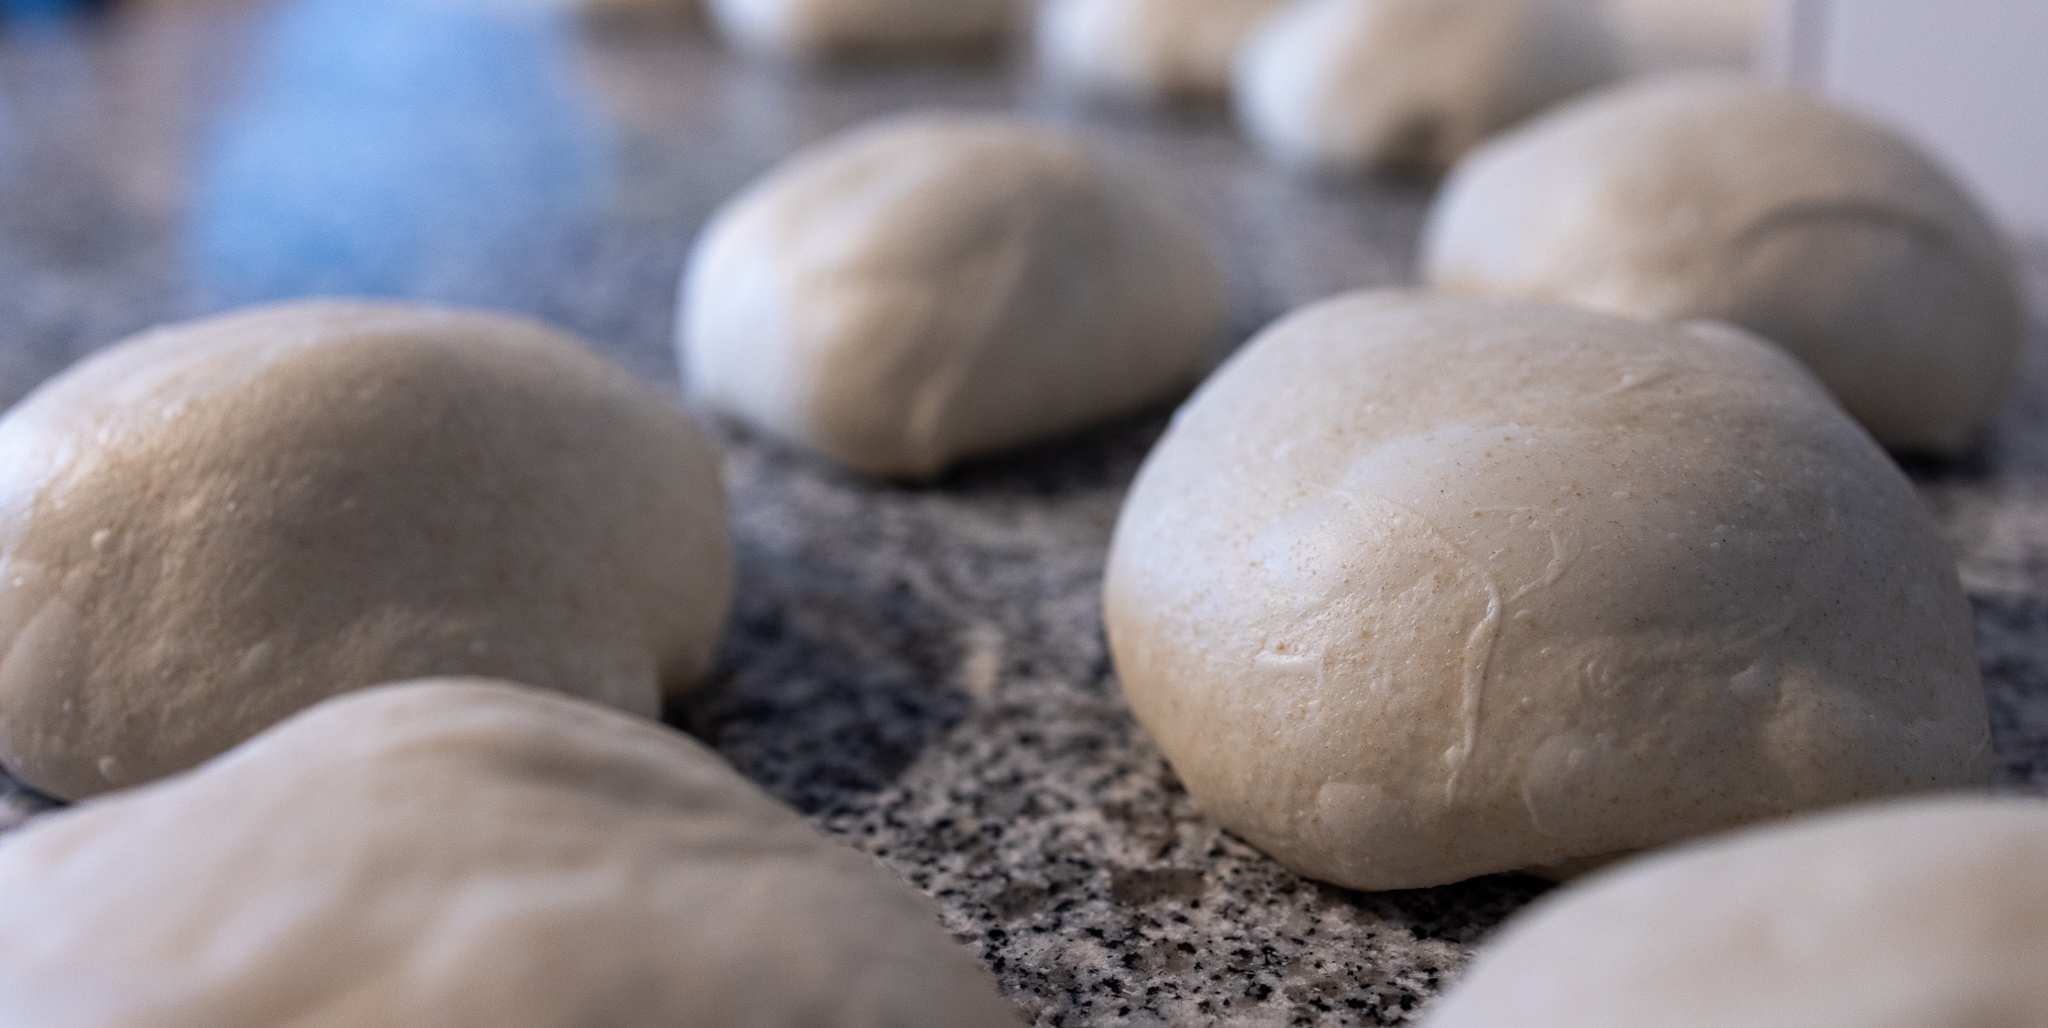
\includegraphics[width=\textwidth]{preshaped-dough}
  \caption{Baguette doughs resting after preshaping.}%
  \label{fig:dough-after-preshaping}
\end{figure}

Once you finished pre-shaping allow the dough balls to rest
on your counter for at least 10--15~minutes. Do not
cover the pre-shaped balls. By drying out the surface,
the following shaping step will be easier. The dried-out surface
will not stick to your hands as much. As
you tightened the dough's gluten you will need to
allow it to relax. Without a resting period, you wouldn't
be able to shape your dough into, for instance, a baguette-like structure.
The dough would resist each movement
always springing back into the previous shape. You
might have noticed this before, when making pizza dough. If you
don't wait long enough after balling the pizzas, it's impossible
to stretch the pizza. By waiting a few more minutes,
stretching becomes a lot easier. The dough will not resist
being transformed into the final shape that you like.

The aforementioned 10--15~minutes bench rest time depends
on how strongly you pre-shaped your dough. The more
you pre-shape the longer you need to wait. If your dough
resists a lot during shaping, extend this period up to 30~minutes.
If you wait too long, your dough's surface area can become too dry,
resulting in the dough tearing during shaping. As always, please
take these timings with a grain of salt and experiment in
your environment.

\section{Shaping}

\begin{flowchart}[!htb]
\centering
  \begin{tikzpicture}[node distance = 3cm, auto]
  \node [block] (init) {\footnotesize Begin shaping};
  \node [decision, right of=init, node distance=5cm] (overfermented_decision) {\footnotesize Dough overly sticky or dough tears?};
  \node [block, right of=overfermented_decision, node distance=4cm] (overfermented) {\footnotesize Your dough is likely overfermented};
  \node [block, right of=overfermented, node distance=3cm] (loafpan) {\footnotesize Move to loaf pan, short proof, then bake directly};
  \node [block, below of=init, node distance=4cm] (shaping_technique) {\footnotesize Proceed with shaping technique};
  \node [block, right of=shaping_technique, node distance=3cm] (flour) {\footnotesize Flour shaped dough};
  \node [block, right of=flour, node distance=3cm] (banneton) {\footnotesize Place upside down in banneton};
  \node [block, right of=banneton, node distance=3cm] (proof) {\footnotesize Begin proofing};
  \path [line] (init) -- (overfermented_decision);
  \path [line] (overfermented_decision) -- node{yes} (overfermented);
  \path [line] (overfermented_decision) -- node{no} (shaping_technique);
  \path [line] (shaping_technique) -- (flour);
  \path [line] (flour) -- (banneton);
  \path [line] (banneton) -- (proof);
  \path [line] (overfermented) -- (loafpan);
\end{tikzpicture}

  \caption[Sourdough shaping process]{A schematic visualization of the shaping process
      including checks for an overfermented dough.}%
  \label{fig:shaping-decision-tree}
\end{flowchart}

Shaping will give your dough the final shape before baking. After
completing shaping, your dough proceeds to the proofing stage and
will then be scored and ultimately baked.

There are countless shaping techniques. The technique to choose
depends on the type of bread you want to make. Some techniques
are gentler on the dough, making sure that the dough does not
degas. Other techniques are faster but degas the dough a little
more. The tighter you shape, the more evened out your final dough's
crumb structure will look. At the same time, a tighter shaping-technique
will improve your dough's strength. More strength will ultimately result
in more vertical oven spring.

The following instructions assume that you want to make a batard-style
bread featuring an oblong shape. Learning this technique
will provide you with a solid knowledge foundation that
can easily be extended to make bread rolls or baguettes.

Mastering the challenging shaping technique will likely take you
multiple attempts. You only have a single attempt per dough, though. If you
make a mistake, the final bread is likely not going to turn out as good
as it could. If this technique causes you a headache, I~recommend making
a larger batch of dough and dividing and preshaping it into
smaller portions. Instead of making a large batard, practice making miniature
batard bread rolls.

\subsection[Flouring the surface]{Apply flour to the dough's surface.}

\begin{figure}[!htb]
  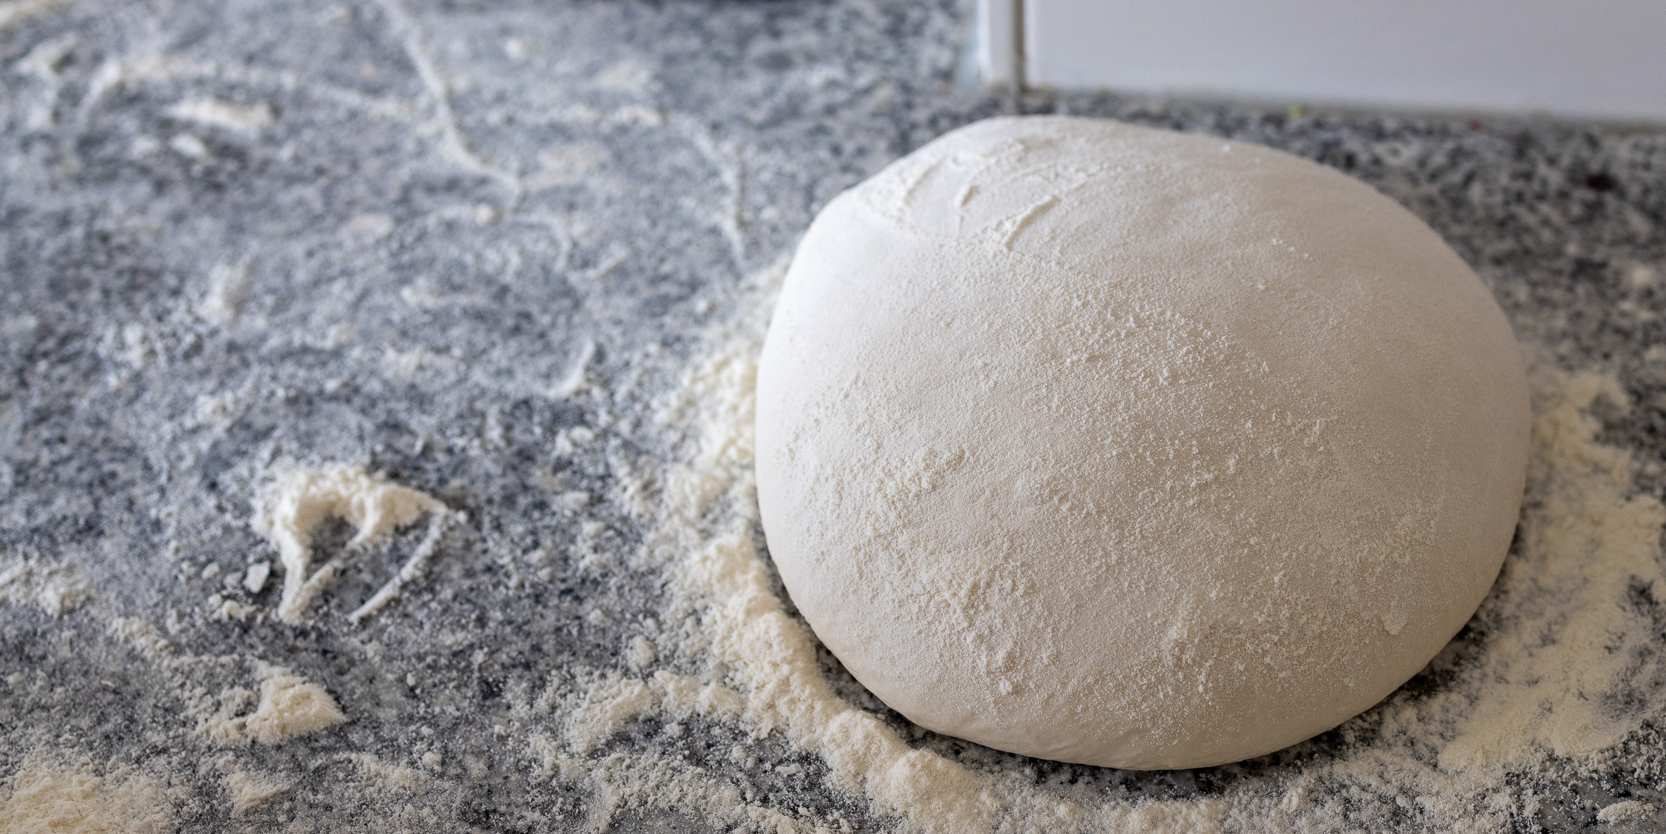
\includegraphics[width=\textwidth]{step-1-flour-applied}
  \caption[Step 1 of shaping process]{A dough that has flour applied to its
      surface. This is the first step of the shaping process.}%
  \label{fig:shaping-flour-surface}
\end{figure}

If you are only making 1 loaf out of your dough, apply flour
generously to the top layer of your dough. Rub the flour onto your
dough with your hands. Flip over your container. Wait a little bit
to allow the dough to release itself from the container. Proceed
with step 3.

If you divided and pre-shaped, apply flour generously to the dough's
top layer as well. With gentle hands spread the flour evenly across
the dough's surface. See figure~\ref{fig:shaping-flour-surface} for a
visual representation of how your dough should look after coating
the surface.

\subsection[Flipping the dough]{Flip the dough over}

\begin{figure}[!htb]
  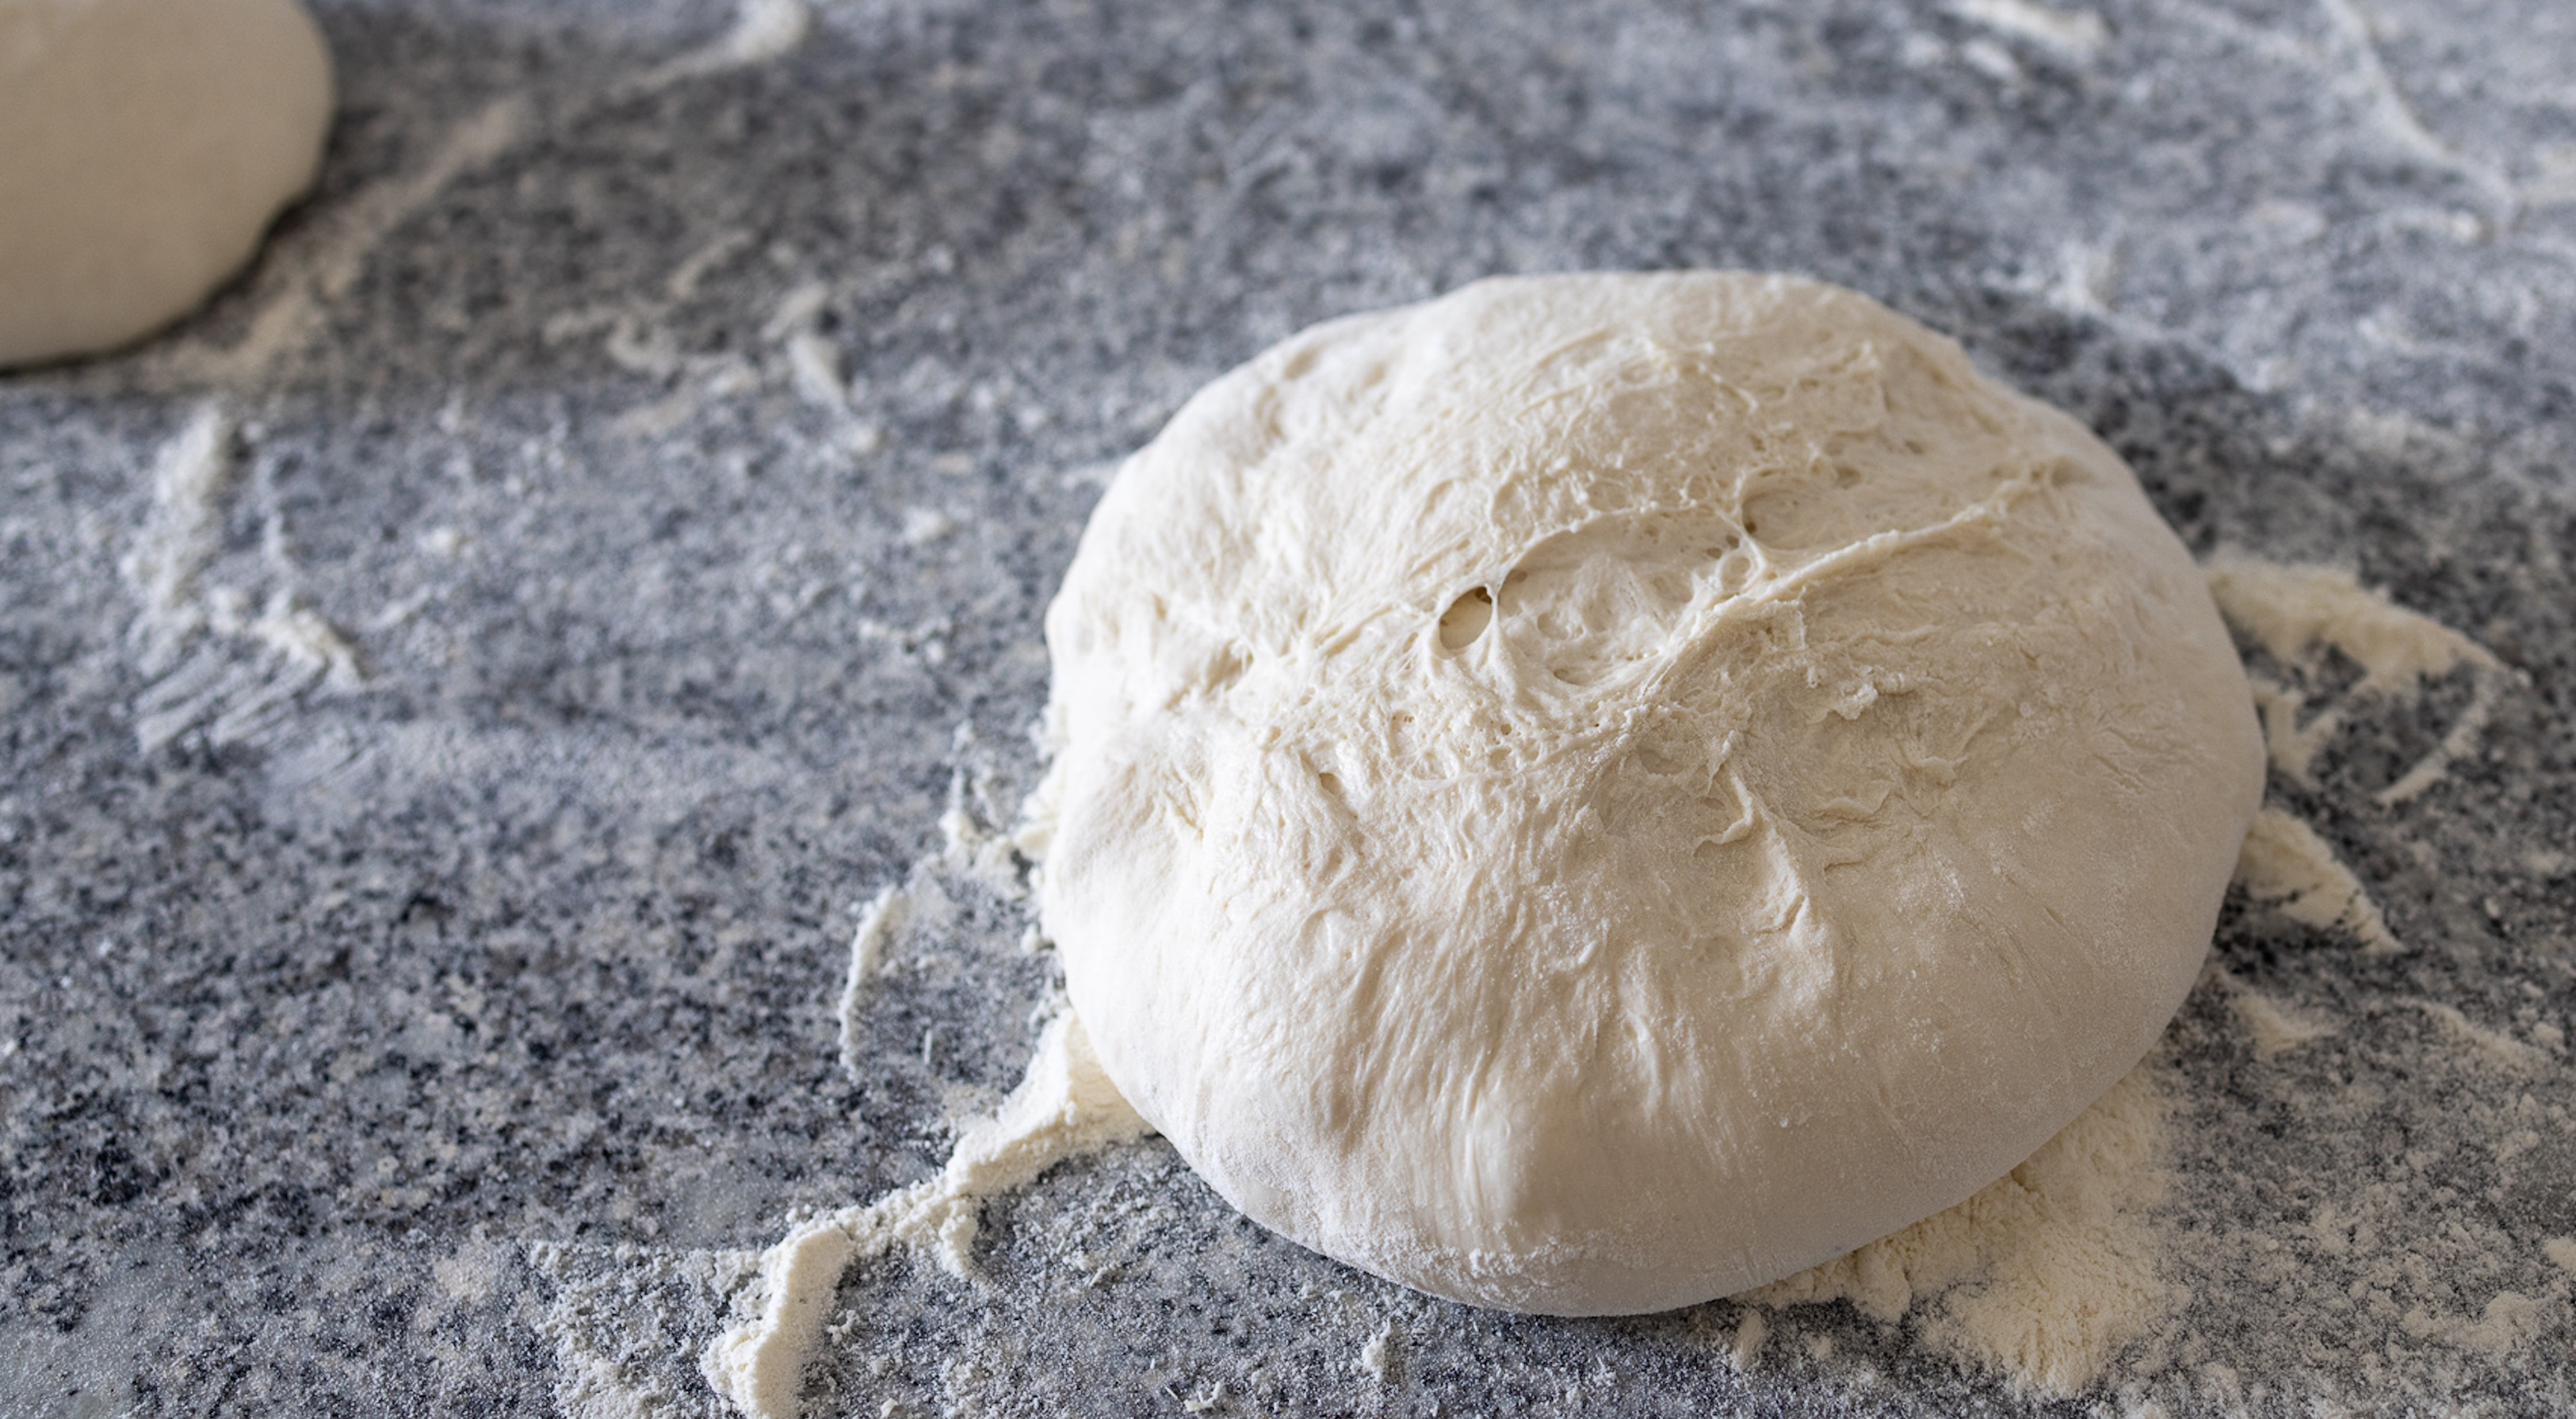
\includegraphics[width=\textwidth]{step-2-flipped-over}
  \caption[Step 2 of shaping process]{A flipped-over dough. Note how the
      sticky side is facing you while the floured side is facing the
      countertop.  The sticky side is used as glue to hold the dough together.}
\end{figure}

With gentle hands, carefully remove the dough from the surface. If
you possess a dough scraper, carefully tuck it under the dough with
rapid movements. Flip the dough over, making sure that the floured
areas are in contact with your hands. The non-floured bottom area that was
stuck to the counter is a no-touch zone. Try to avoid touching it
as it is rough and thus will stick to your hands.

Gently proceed and place the dough with the previously top-facing side
on your counter. The floured area is now on the surface, whereas the
sticky side is facing you.

\subsection[Create rectangular shape]{Make the dough rectangular}

\begin{figure}[htb!]
  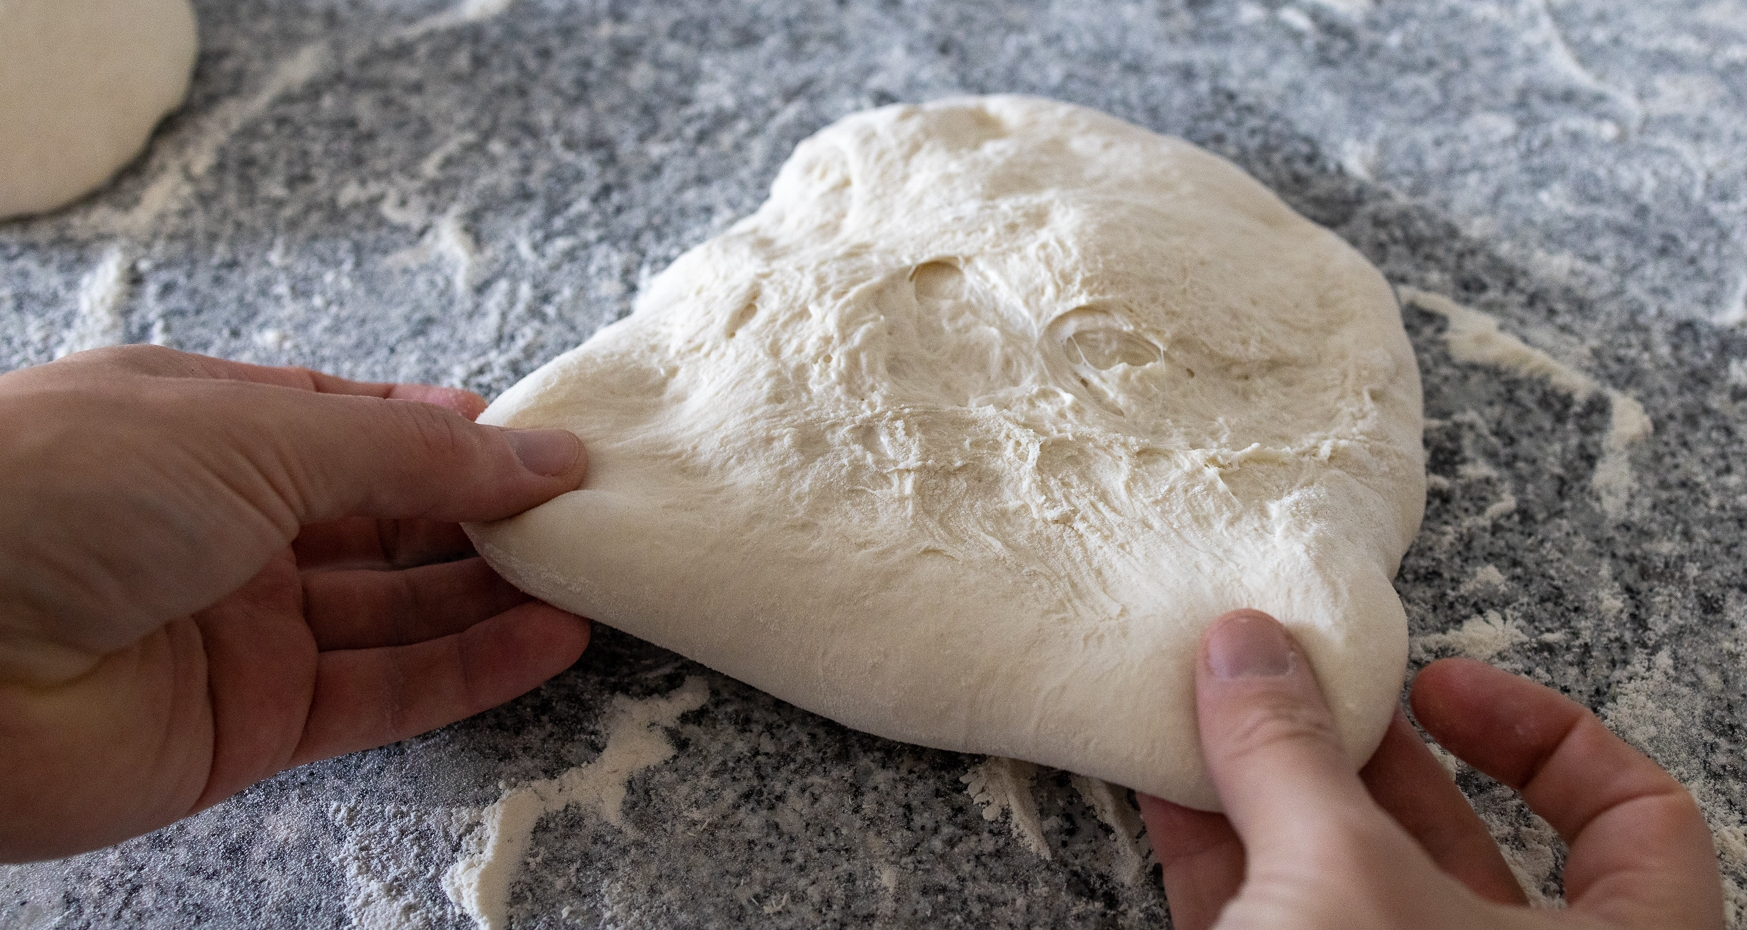
\includegraphics[width=\textwidth]{step-3-rectangular}
  \caption[Step 3 of shaping process]{A flipped-over dough. Note how the
      sticky side is facing you while the floured side is facing the
      countertop.}%
  \label{fig:shaping-rectangular-dough}
\end{figure}

You should be facing the sticky side of your dough now. Note how
the dough is currently round and not rectangular. The circular
shape will not be ideal when shaping the oblong batard.

For this reason, proceed and stretch the dough a little bit until
it has a more rectangular shape. While stretching, make sure to touch
the sticky side as little as possible. Place your hands on the bottom
floured side and the edge of the sticky side. With gentle hands,
stretch the dough until the shape in front of you looks rectangular.
Refer to figure~\ref{fig:shaping-rectangular-dough} and compare
your dough with the shown dough.

\subsection[Folding]{Fold the dough together}

\begin{figure}[htb!]
  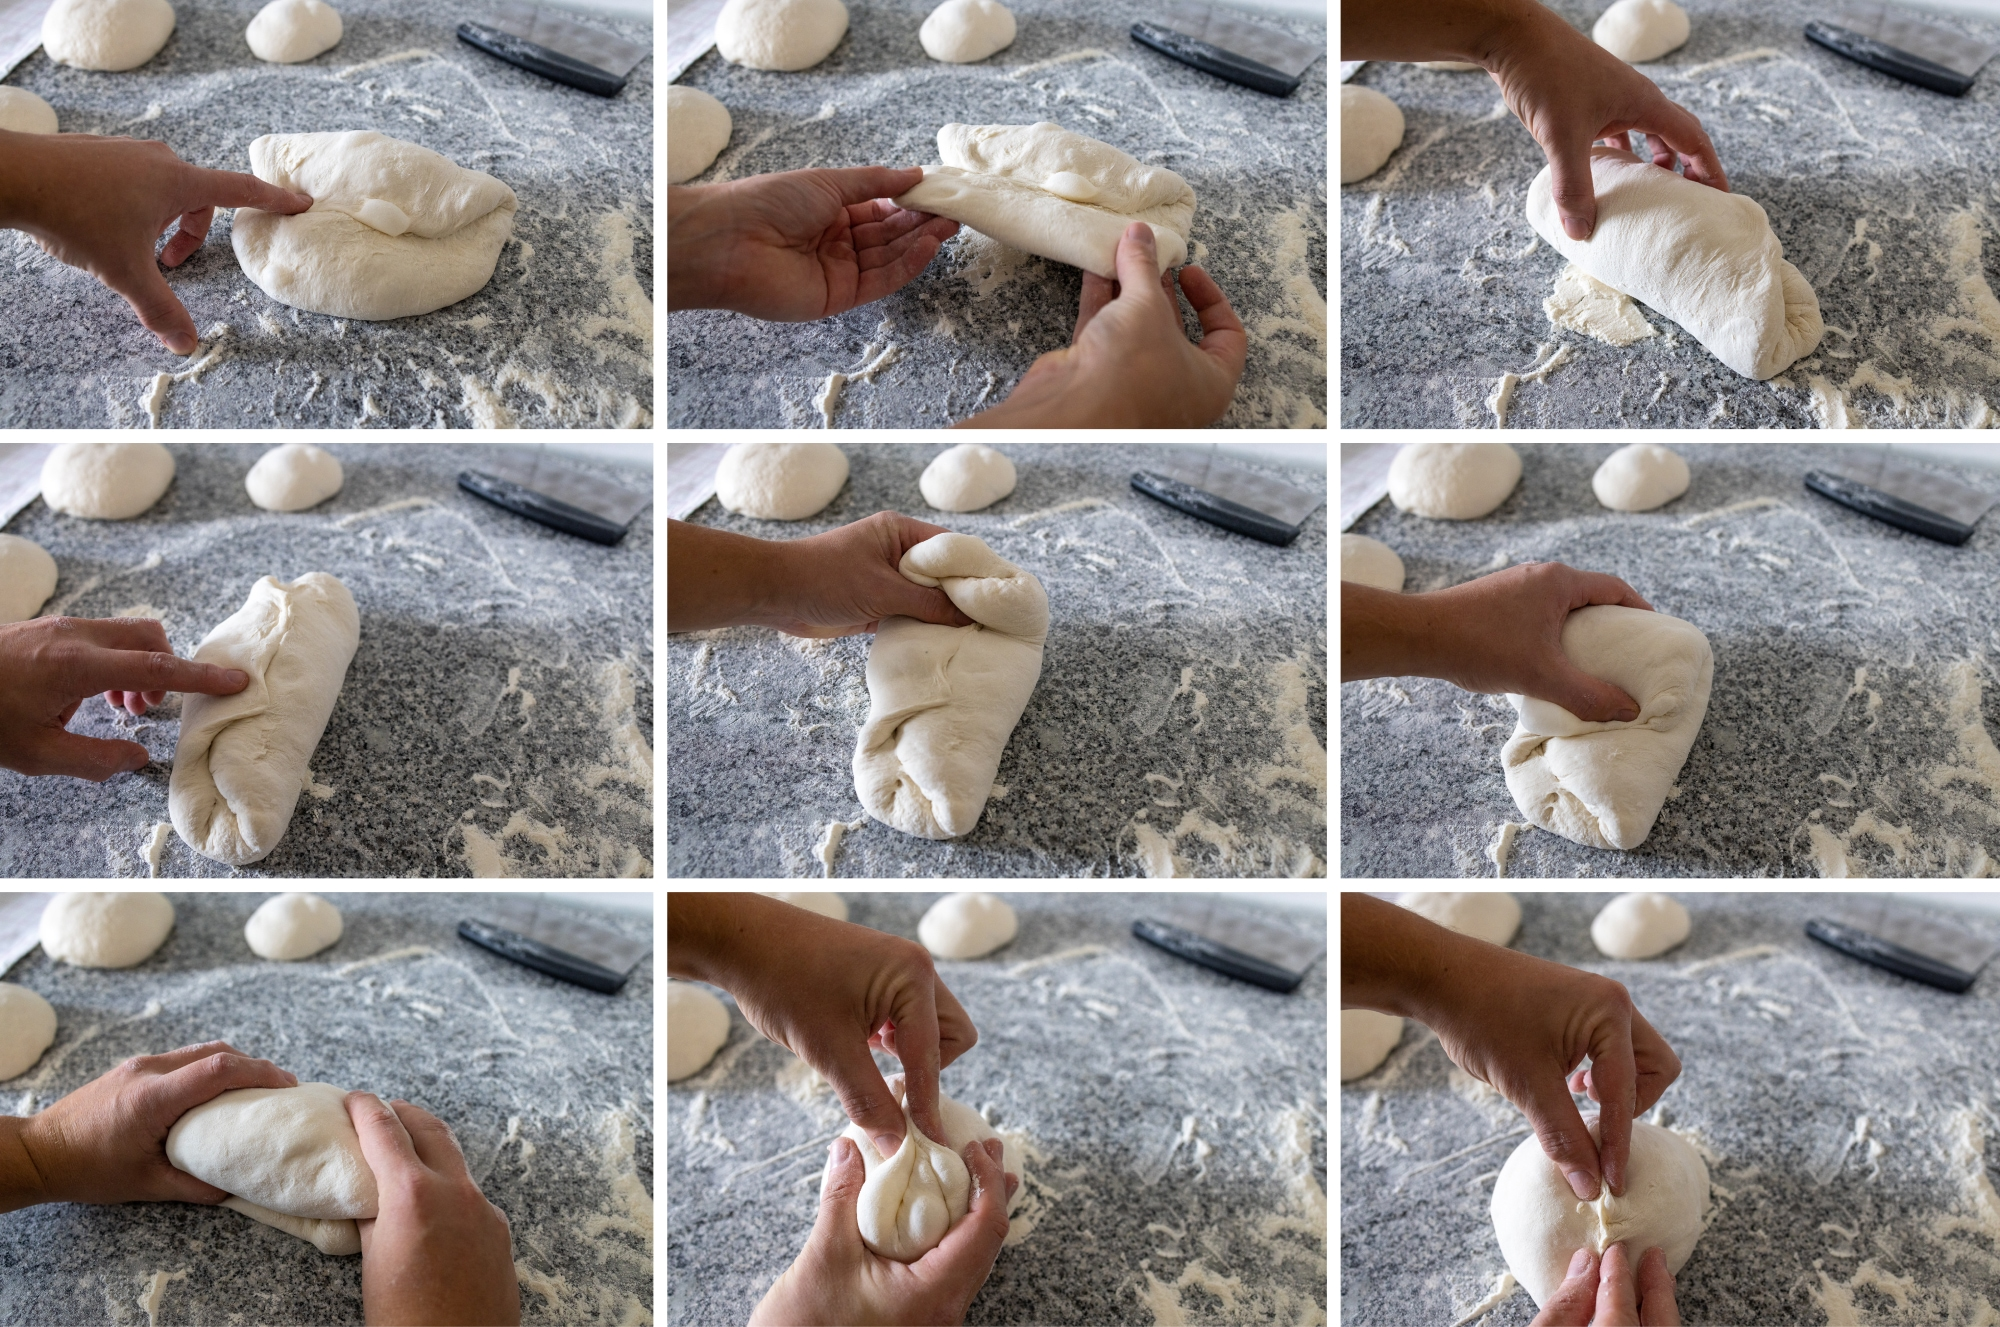
\includegraphics[width=\textwidth]{step-4-folding}
  \caption[Step 4 of shaping process]{The process of folding a batard. Note
      how the rectangle is first glued together and then rolled inwards to
      create a dough roll. Ultimately the edges are sealed to create a more
      uniform dough.}%
  \label{fig:shaping-folding}
\end{figure}

Now that you have created the rectangular shape, your dough
is ready to be folded together. This only works because the side
facing you is sticky. Because of the dough's stickiness,
we can effectively glue it together, creating a very
strong bond.

You can practice this step with a piece of rectangular paper.
Once you mastered folding on paper you can easily apply
this to your real-life dough.

Make sure the batard is placed in front of you. Take the side
that faces you and fold it into the middle of the dough. Carefully
tuck it down so that it glues together with the sticky side.

Take the other side and fold it over the side you just folded.
Stretch the dough as much as possible towards you. Tuck it down
on the edge, creating your first glue layer.

Rotate the dough so that it is aligned lengthwise in front of you.
Rotate the dough inwards so that the seam side
now faces you.

Start to roll the dough inwards beginning at the top of the dough.
Keep rolling the dough inwards until you have created a dough roll.

Refer to figure~\ref{fig:shaping-folding} for a full visual
representation of the process.

If your dough does not hold its shape, chances are you have pushed
the fermentation too far. Most of the gluten has been degraded
and the dough won't be able to hold its shape. In this case,
the best option is to use a loaf pan to bake your bread. The
final bread will taste amazing but not offer the same texture
a freestanding bread would offer. Please refer to
Section~\ref{section:debugging-crumb-structure} for more
details on how to properly read your dough's crumb structure.

\subsection[Sealing]{Sealing the edges}

Your dough has finished shaping now. Sealing the edges
is an optional step. I~like to do it because, in my opinion,
the final baked bread will look a little bit nicer without
any rough edges.

Gently pull together the swirl-like-looking edges of your dough
with two fingers. Rotate the dough and then repeat the same process
from the other side as well.

\subsection[Proofing preparation]{Prepare for proofing}

\begin{figure}[htb!]
  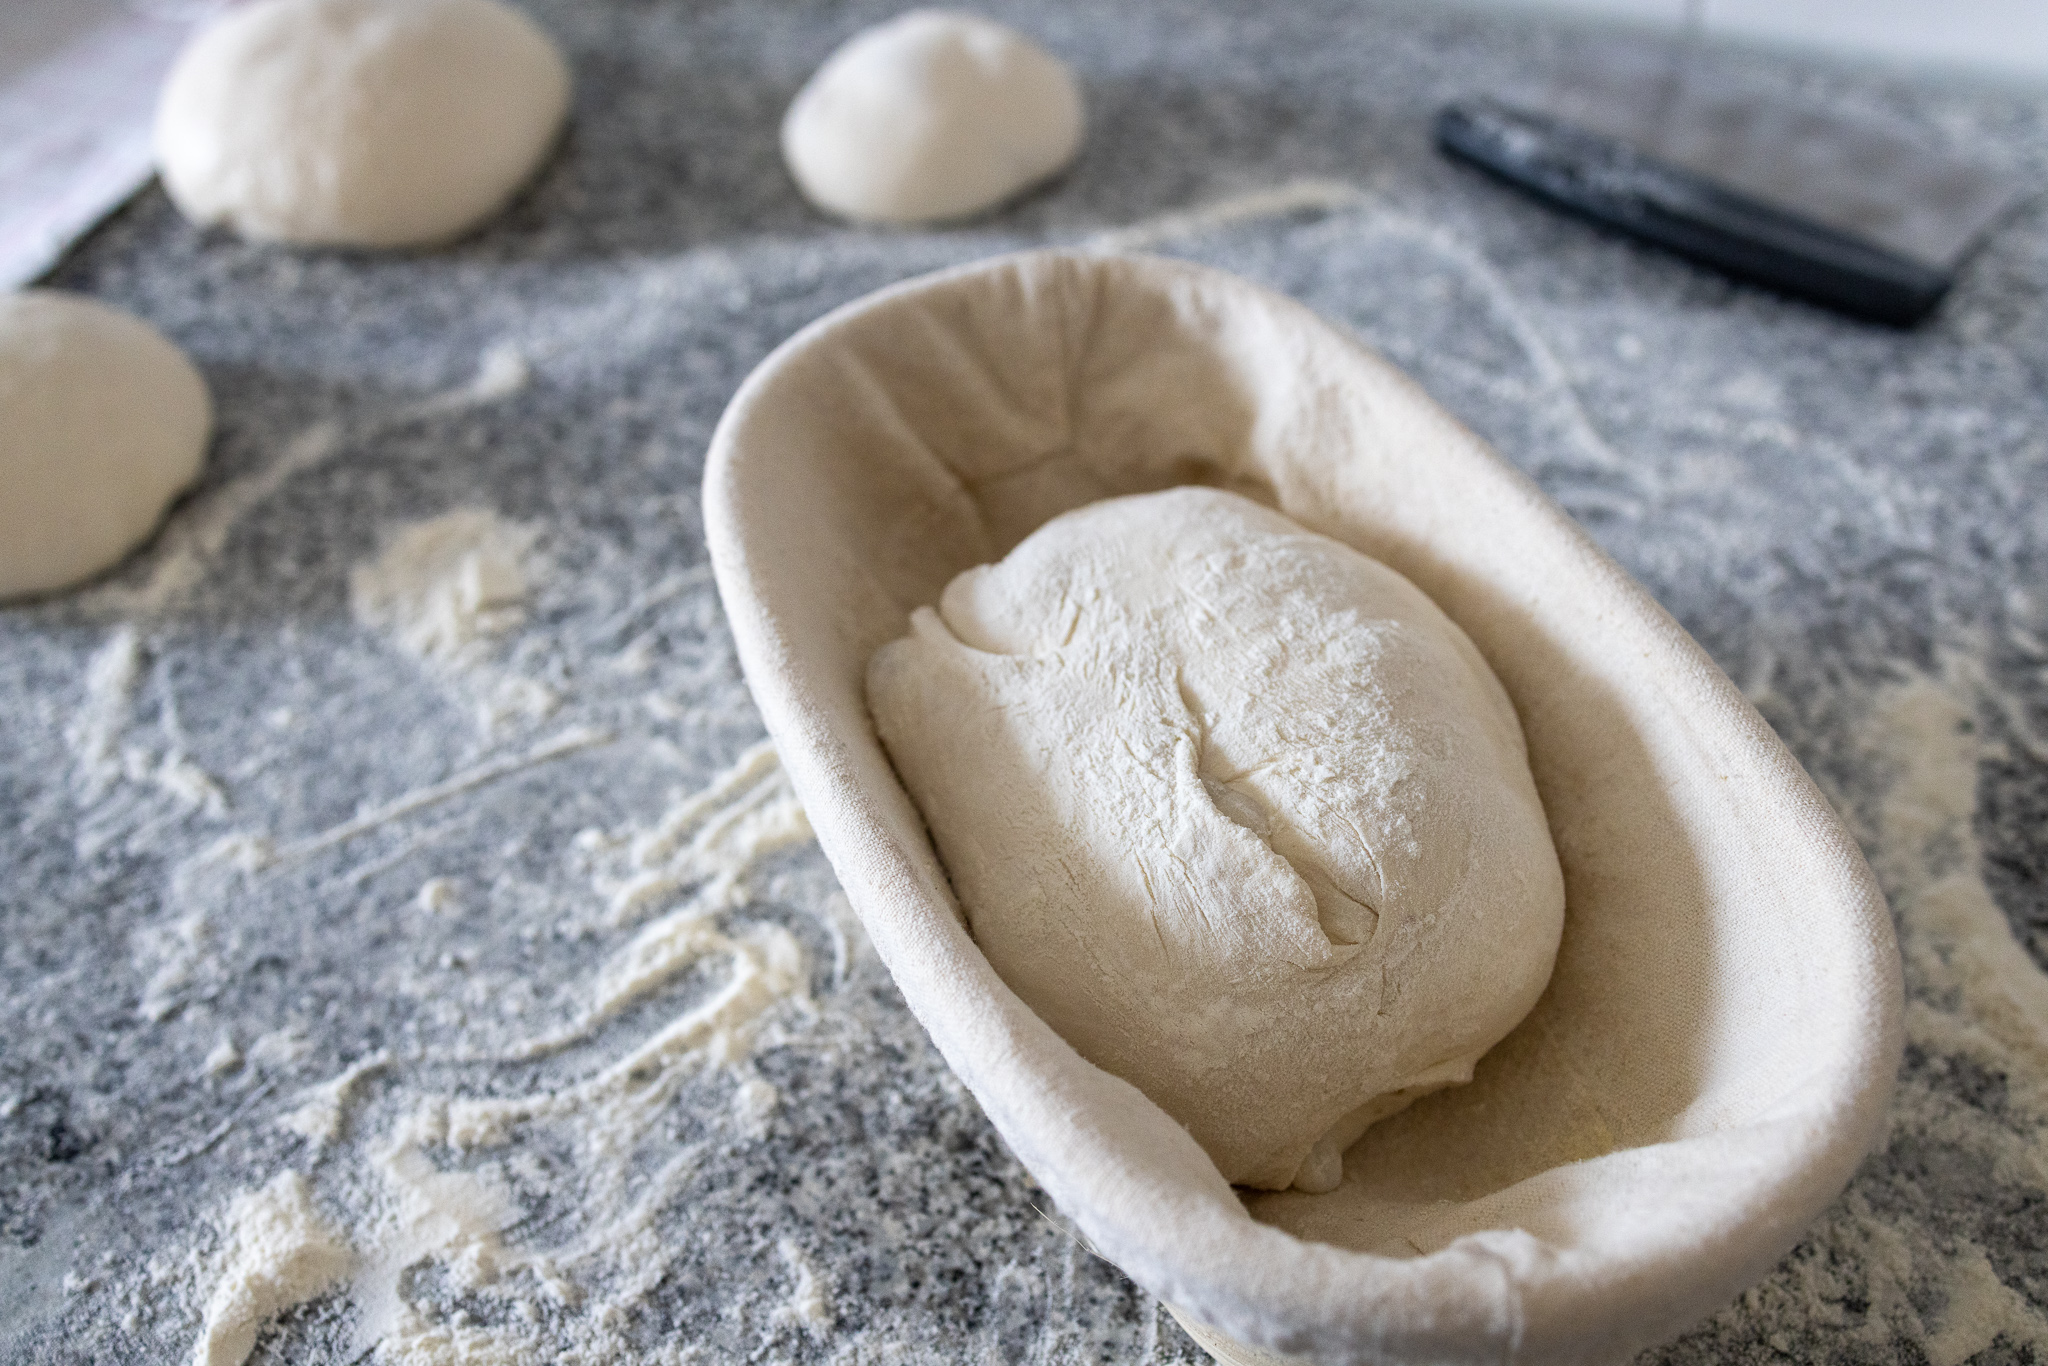
\includegraphics[width=\textwidth]{step-6-prepare-proofing}
  \caption[Step 5 of shaping process]{The shaped dough is ready for proofing
      in the banneton. Note how the seam side is now facing you. The floured
      previous top side is facing downwards.}%
  \label{fig:shaping-prepare-proofing}
\end{figure}

You should have a beautifully shaped dough in front of you now.
The proofing stage is about to start. To simplify later
scoring and to make sure your dough won't stick to your banneton,
apply another flour rub to the dough's surface. This
will dry out the surface and reduce the dough's tendency
to stick to everything.

For the coating, I~recommend using the same flour you used
to make your dough. Rice flour is only recommended if you
want to apply artistic scoring patterns later. It is better
to use more flour than too little flour. Excess flour can be
brushed off later.

Once your dough has been coated, it is ready to be placed on your banneton.
If you do not have a banneton, you can use a bowl
with a kitchen towel inside.

The currently top-facing floured surface will be downwards-facing in your banneton.
By doing so the banneton can be flipped
over before baking, releasing the dough\footnote{The same
applies when making other doughs such as baguette doughs. The floured
surface will always be downwards facing. The dough is then flipped over
once for baking.}.

Proceed and lift the dough with 2 hands from the counter.
Gently rotate it once and then place the dough in your
banneton for proofing\footnote{The seam side should now be facing you.
Some bakers like to seal the seam a little more. I~did
not notice that this improves the dough's strength. As far as I~can
tell, this only improves the visual appearance of the bottom side
of the final loaf.}. If you did everything right, then your
dough should look somewhat similar to the dough shown in figure~\ref{fig:shaping-prepare-proofing}.
As the last step of shaping, place a kitchen towel over your banneton
or bowl and begin proofing.

\section{Proofing}

In bread baking, proofing refers to the final rise of dough before baking,
after it has been shaped into a loaf. The chemical reactions and processes
that occur during bulk fermentation and proofing are the same.

By shaping your dough, it has lost some of the air previously generated
throughout the bulk fermentation. The goal of proofing is to inflate
the dough again. A dough without proofing wouldn't offer the same texture
as a properly proofed dough. The proofed dough features a very fluffy
and soft crumb.

There are two proofing techniques. One strategy is to proof the dough
at room temperature whereas the other proofs the dough in the fridge.
Fridge-proofing is also commonly known as retarding.

Some bakers claim that cold-proofing improves the final flavor of the bread.
In all the loaves that I~retarded I~could not tell a difference
in terms of flavor for cold-proofed doughs. The microorganisms work
at a slower rate at colder temperatures. But I~doubt that they alter
their biochemical processes. More research is needed on the topic
of retarding and flavor development.

\begin{flowchart}[!htb]
\centering
  \begin{tikzpicture}[node distance = 3cm, auto]
  \node [decision] (init) {\footnotesize Room temperature proofing?};
  \node [decision, right of=init, node distance=9cm] (retard_bake_decision) {\footnotesize Bake in less than 10 hours from now?};
  \node [block, below of=init, node distance=4cm] (poke) {\footnotesize Poke the dough};
  \node [block, right of=poke, node distance=4cm] (wait_poke) {\footnotesize Wait 15 minutes};
  \node [decision, below of=poke, node distance=3cm] (dent_visible_decision) {\footnotesize Dent still visible after 1 minute?};
  \node [block, right of=dent_visible_decision, node distance=4cm] (bake) {\footnotesize Score and bake};
  \node [block, below of=retard_bake_decision, node distance=3cm] (wait_retard) {\footnotesize Wait 15 minutes};
  \node [block, below of=wait_retard, node distance=3cm] (retard) {\footnotesize Proof in fridge at 4°C (40°F)};
  \node [block, right of=wait_retard, node distance=3cm] (move_to_fridge) {\footnotesize Move dough directly to fridge};
  \path [line] (init) -- node{yes} (poke);
  \path [line] (init) -- node{no} (retard_bake_decision);
  \path [line] (poke) -- (dent_visible_decision);
  \path [line] (dent_visible_decision) -- node{yes} (bake);
  \path [line] (dent_visible_decision) -- node{no} (wait_poke);
  \path [line] (wait_poke) -- (poke);
  \path [line] (retard_bake_decision) -- node{yes} (wait_retard);
  \path [line] (retard_bake_decision) -- node{no} (move_to_fridge);
  \path [line] (wait_retard) -- (retard);
  \path [line] (move_to_fridge) -- (retard);
  \path [line] (retard) -- (bake);
\end{tikzpicture}

  \caption[Sourdough proofing process]{A schematic overview of the different steps of
      the sourdough proofing process. The proofing technique to choose depends
      on your availability and schedule.}%
  \label{fig:proofing-process}
\end{flowchart}

To me, the sole purpose of cold-proofing is its ability to allow you
to better manage the timing of the whole process. Assuming you finished shaping
your dough at 10 pm, chances are you wouldn't want to wait for another
2~hours to proof the dough and then another 1 hour to bake it. In this case,
you can move your dough directly to the fridge after shaping. Your
dough will be proofing overnight in the fridge. Then it can be baked at any time
the following day (there are a few exceptions; more on that later).
This is especially handy for large-scale bakeries that use fridge-proofing
extensively. Some of the doughs are proofed a day before and placed in the fridge.
Early in the morning, they can be baked directly out of the fridge. Within 2
hours they will be ready to sell the first bread to morning customers. If
throughout the day more bread is needed, they simply take some proofed dough out
of the fridge and bake it. The time frame in which you can bake retarded
dough is big. It can be as little as 6~hours later up to 24~hours later.

Assuming you made an overnight dough and your dough is ready in the morning,
the situation might be different. You potentially want to bake the dough directly
for breakfast, or at lunchtime. In this case, you wouldn't want to proof the dough for
another 6~hours in the fridge. Room temperature-proofing is your technique
of choice.

To summarize, choose the technique that works for you depending on your
schedule and availability.

\subsection{Room temperature-proofing}

The easiest and most reliable way to proof your dough is to proof the dough at
room temperature. It is my method of choice if my schedule allows it. This method
works great if you make an overnight dough and then proof it the next
morning.

\begin{figure}[htb!]
  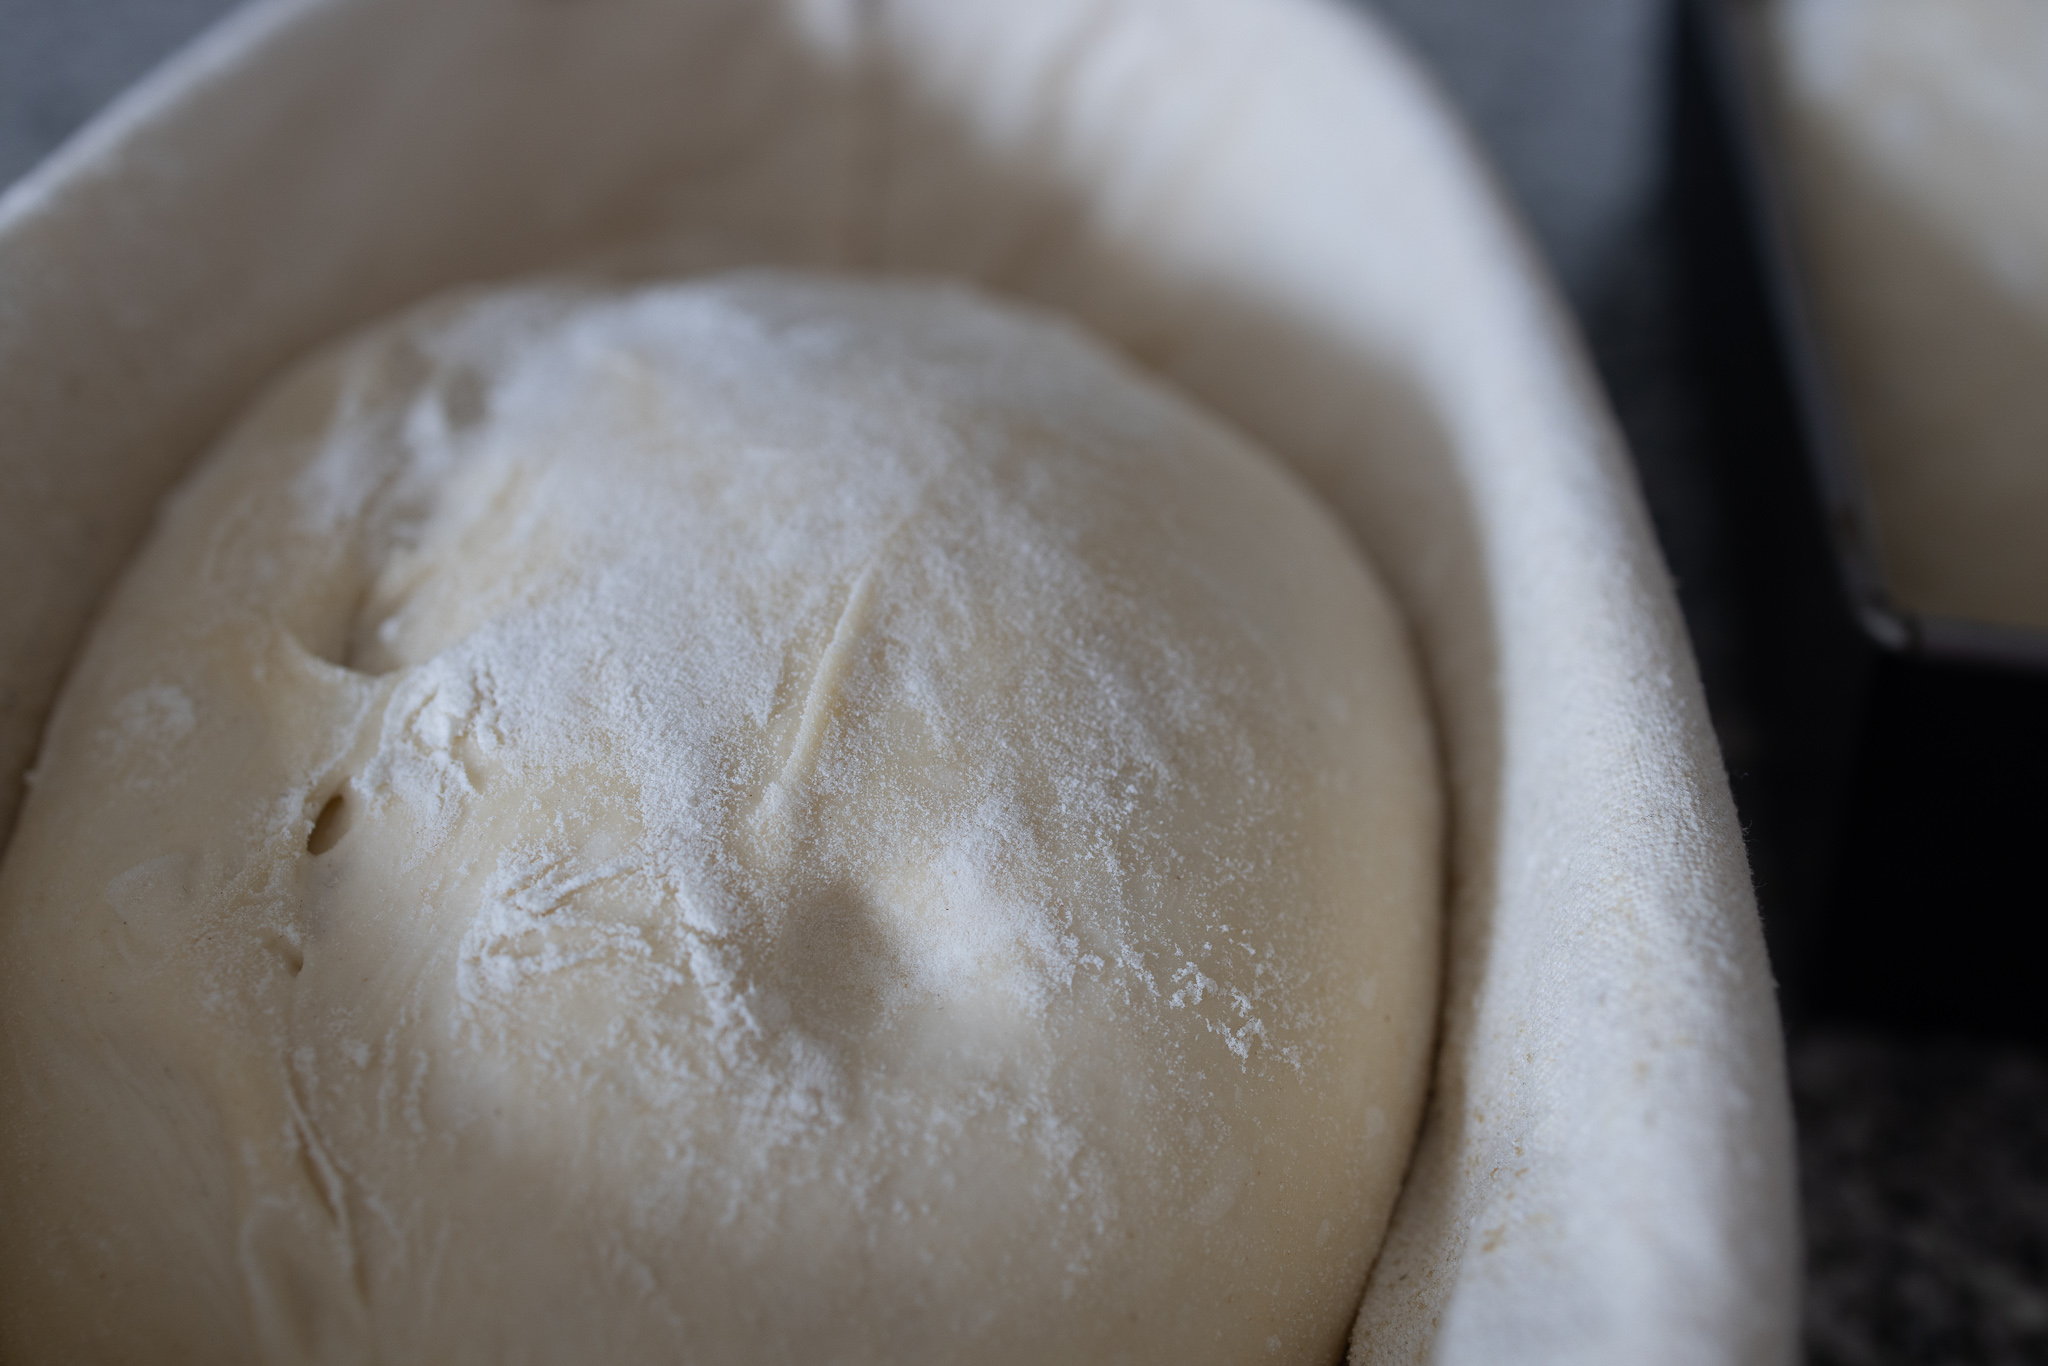
\includegraphics[width=\textwidth]{step-13-finger-poke-test}
  \caption[The finger poke test]{The finger poke test is a very reliable
      method to check if your dough has been properly proofed. If the induced
      dent is still visible one minute later, your dough can be baked.}%
  \label{fig:shaping-finger-poke}
\end{figure}

The time it takes to proof your dough can be anything between 30~minutes and
3~hours. Rather than relying on timing, most bakers use the finger poke test.

Flour your thumb and gently press around 0.5cm up to 1cm deep into the dough.
Try this directly after shaping. You will notice that the created dent will
recover quickly. It will be gone again after 1 minute.

As you proceed with proofing, your dough will fill up with more gas. At the
same time, the dough will become more extensible. Once it starts to reach the
right amount of fluffiness and extensibility, the dent will disappear more slowly.
Once the dough is ready for scoring and baking the dent should still be visible after
1 minute of waiting.

I~recommend performing the finger poke test once every 15~minutes throughout
the proofing stage. Realistically, based on my experience, proofing takes at least
one hour and can sometimes take up to 3~hours. Even at warmer temperatures proofing
has never been faster than an hour for me. As always please take my timings with
a grain of salt and experiment on your own.

Once I~see that the dough is getting close to perfect proofing, I~proceed and
preheat my oven. This way I~don't overproof the dough. You would notice an
over-proofed dough when the dough suddenly becomes very sticky. At the same
time, the dough is likely to collapse during baking and will not spring back.
Generally, it is better to end proofing too early rather than too late.

\subsection{Cold-proofing (retarding)}

The second proofing option is to place your dough inside the fridge for
proofing. This option is great if you do not want to bake the dough
within the next 3~hours.

The dough will initially proof at the same rate as the room temperature dough.
As the dough cools down the rate of fermentation slows. Ultimately at below
\qty{4}{\degreeCelsius} (\qty{40}F) the fermentation comes to a halt\footnote{The actual temperature
depends on the bacteria and yeast you cultivated in your sourdough
starter.}. The dough can rest in the fridge for up to 24~hours. In some
experiments, the dough was still good even 48~hours later. Interestingly,
there is a limit to fridge proofing. I~can only explain this with continuous
fermentation activity at low temperatures.

The hard part is to judge when the dough is finished proofing in your fridge.
The previously mentioned finger poke test does not work on cold dough. Low
temperatures change the dough's elasticity. The dent from the poke test
will never recover.

For this reason, finding the best fridge-proofing time is best done
with an iterative approach. Begin with 8~hours on your first dough,
10~hours on the second, 12~hours on the third, and so on up to 24~hours.
As the temperature in your fridge is typically constant, you have an
environment in which you can rely on timings. Find the ideal proofing
time that works for you.

One additional consideration is the dough's core temperature before
placing it inside the fridge. The warmer your dough is initially
the longer it takes for the dough to cool down. This is an additional
variable to take into consideration when choosing the retarding time.
In summer times when my kitchen is hot, I~choose a shorter fridge-proofing
time compared to winter times when the dough is colder.

A reliable way to ensure consistent proofing is to opt for using a pH
meter. By checking the amount of piled-up acidity you can ensure
each of your doughs has the right amount of acidity. Opt for an iterative
approach and check the pH for multiple proofing times. Find the pH
value that creates the best bread for you. Once you have identified
your perfect pH value you can resort to that number on all following
doughs. See Table~\ref{table:sample-ph-values} for some sample pH values
to follow.

\section{Scoring}

Once your dough is done proofing, it's time to warm up your oven
to around \qty{230}{\degreeCelsius} (\qty{446}{\degF}). The next step is then
to proceed with scoring your dough.

Scoring is done for two reasons. There is functional and decorative
scoring. Functional scoring refers to making a small incision in the dough
through which it rises while baking. If the dough is not scored,
it would likely crack open at the weakest spots where you sealed
the dough after shaping. Decorative scoring can be used to apply
artistic patterns to your dough and make it more appealing. When
you want to apply artistic scoring, it is best to rub your dough
with additional rice flour before scoring. The white rice flour
greatly boosts the contrast of the scoring incisions and thus
makes the final pattern look more visually appealing.

\begin{figure}[htb!]
  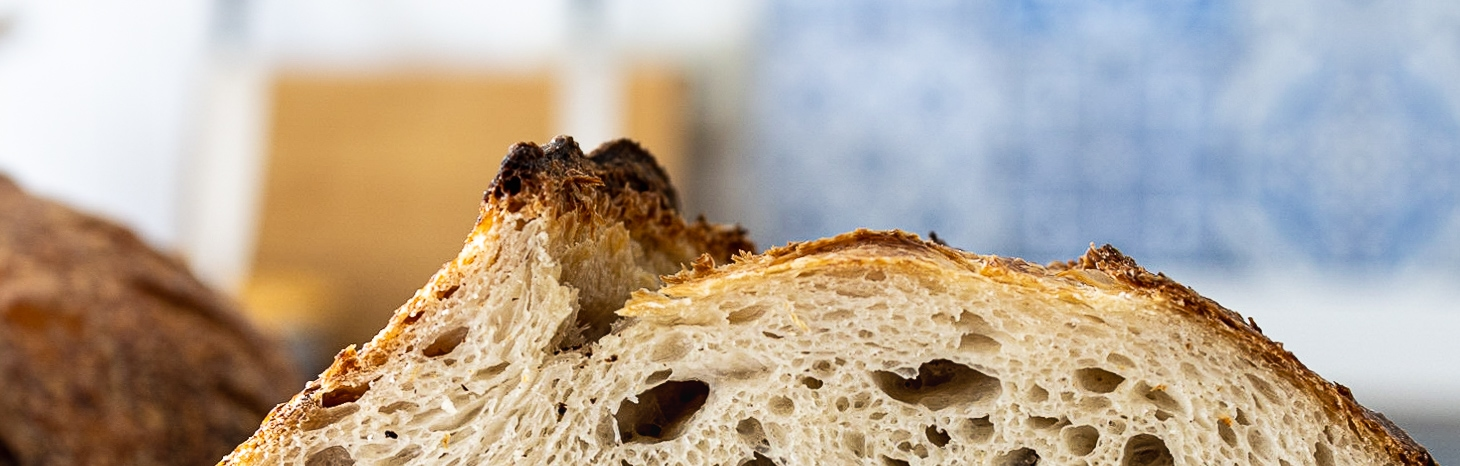
\includegraphics[width=\textwidth]{the-ear}
  \caption[Bread's ear]{The ear is a characteristic that can be achieved on
      wheat sourdough when fermenting and scoring your dough with the perfect
      technique. It offers additional flavor and great texture when eating the
      bread.}%
  \label{fig:the-ear}
\end{figure}

When using a banneton, the dough is flipped over and
placed on an oven rack, tray, stone, steel, or dutch oven. The pros
and cons of the different baking options are covered in the next chapter.
The dough's top side which was previously at the bottom of the
banneton should now be facing you.

\begin{figure}[htb!]
  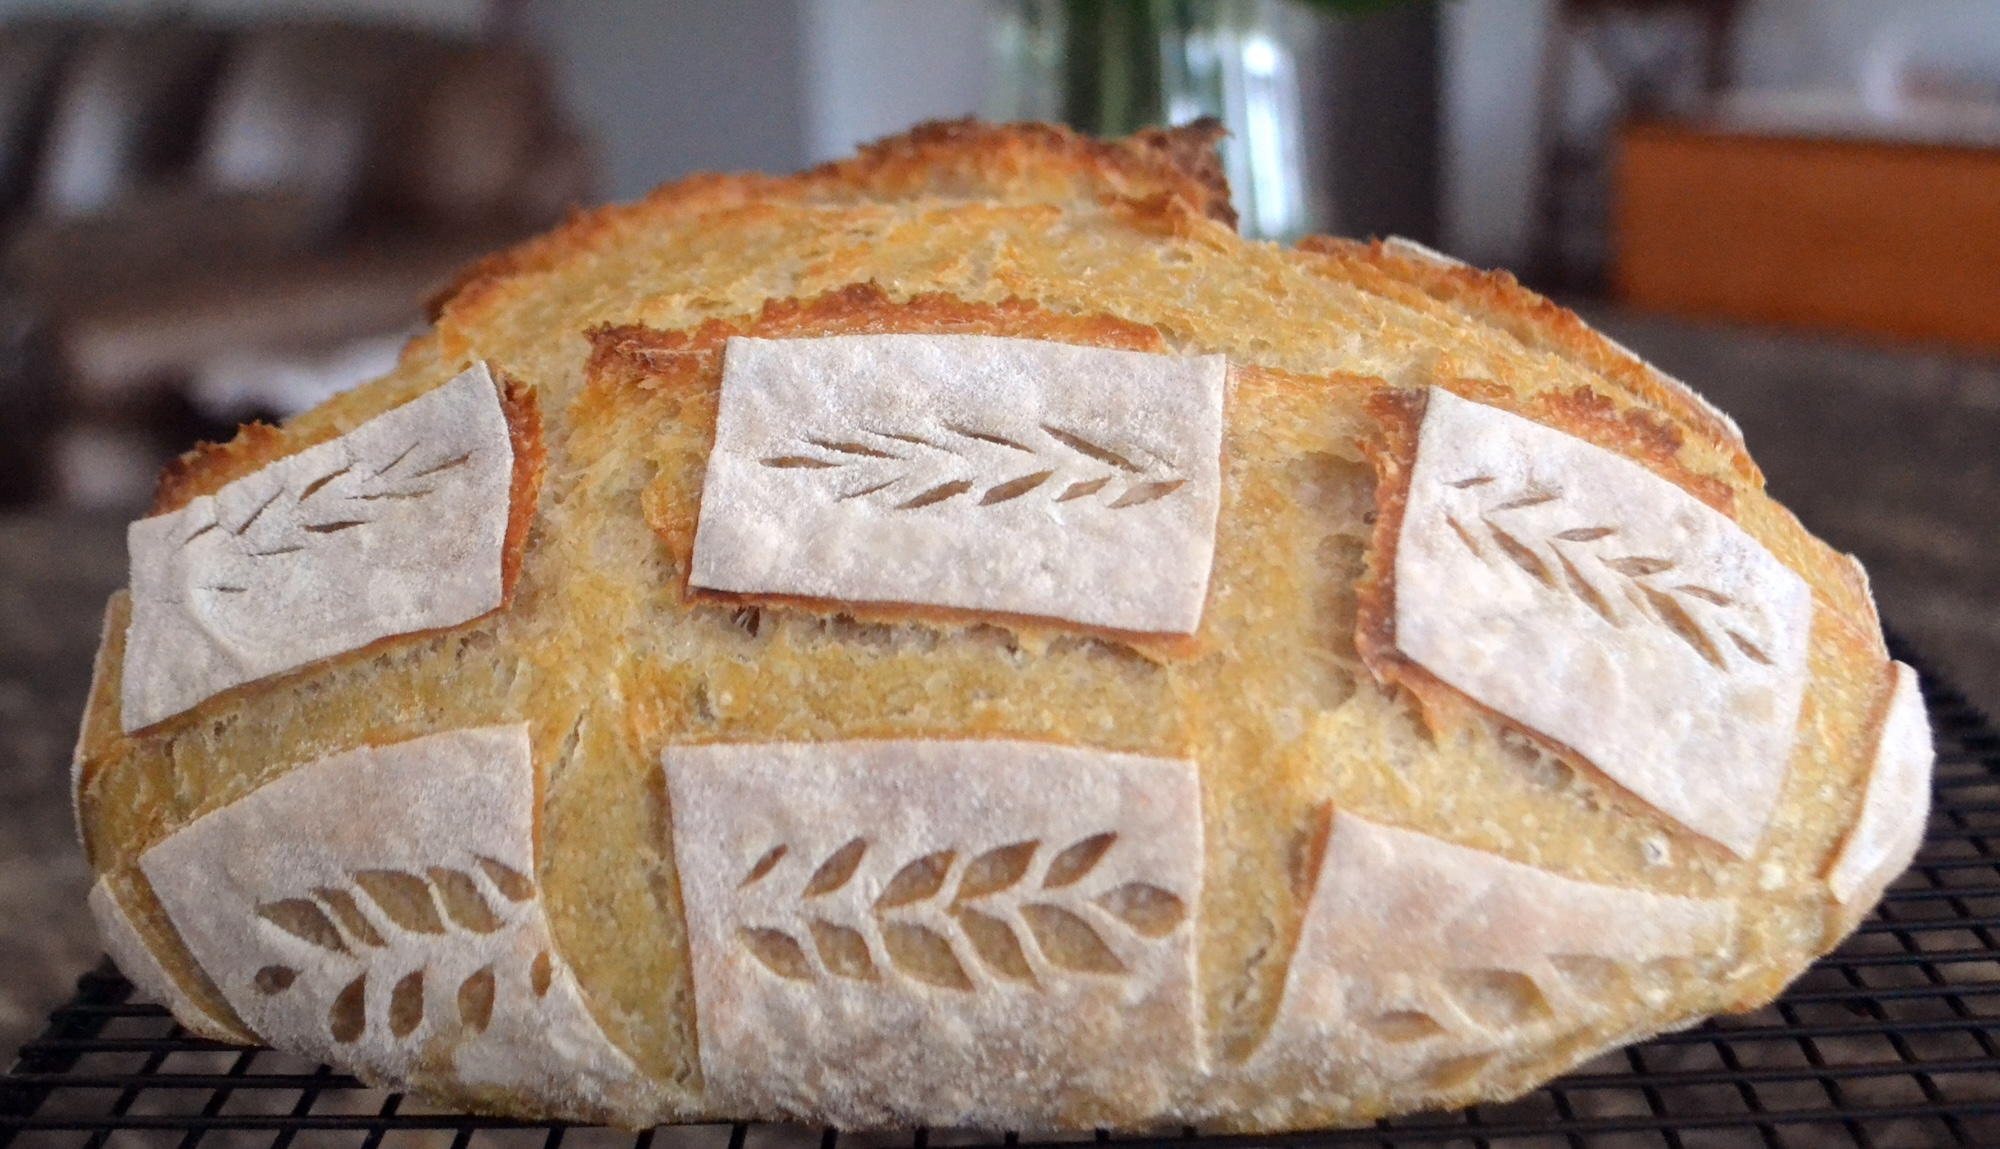
\includegraphics[width=\textwidth]{artistic-scoring}
  \caption[Artistic scoring]{A loaf by Nancy~Anne featuring an artistic
      scoring pattern.  The high contrast was achieved by rubbing the dough's
      surface with rice flour before baking. Her Instagram account
      \texttt{simply.beautiful.sourdough} is specialized to showcase beautiful
      artistic scoring patterns.}%
  \label{fig:artistic-scoring}
\end{figure}

The scoring cut is done at a \ang{45}~angle relative to the dough's
surface slightly off the dough's center. With the \ang{45}~angle cut
the overlaying side will rise more in the oven than the other side.
This way you will achieve a so-called \emph{ear} on the final bread.
The ear is a thin crisp edge that offers intriguing texture
when eating. The thin edge is typically a bit darker after baking
and thus offers additional flavor. In my opinion, the ear turns
a good loaf into a great loaf.

\begin{figure}[htb!]
  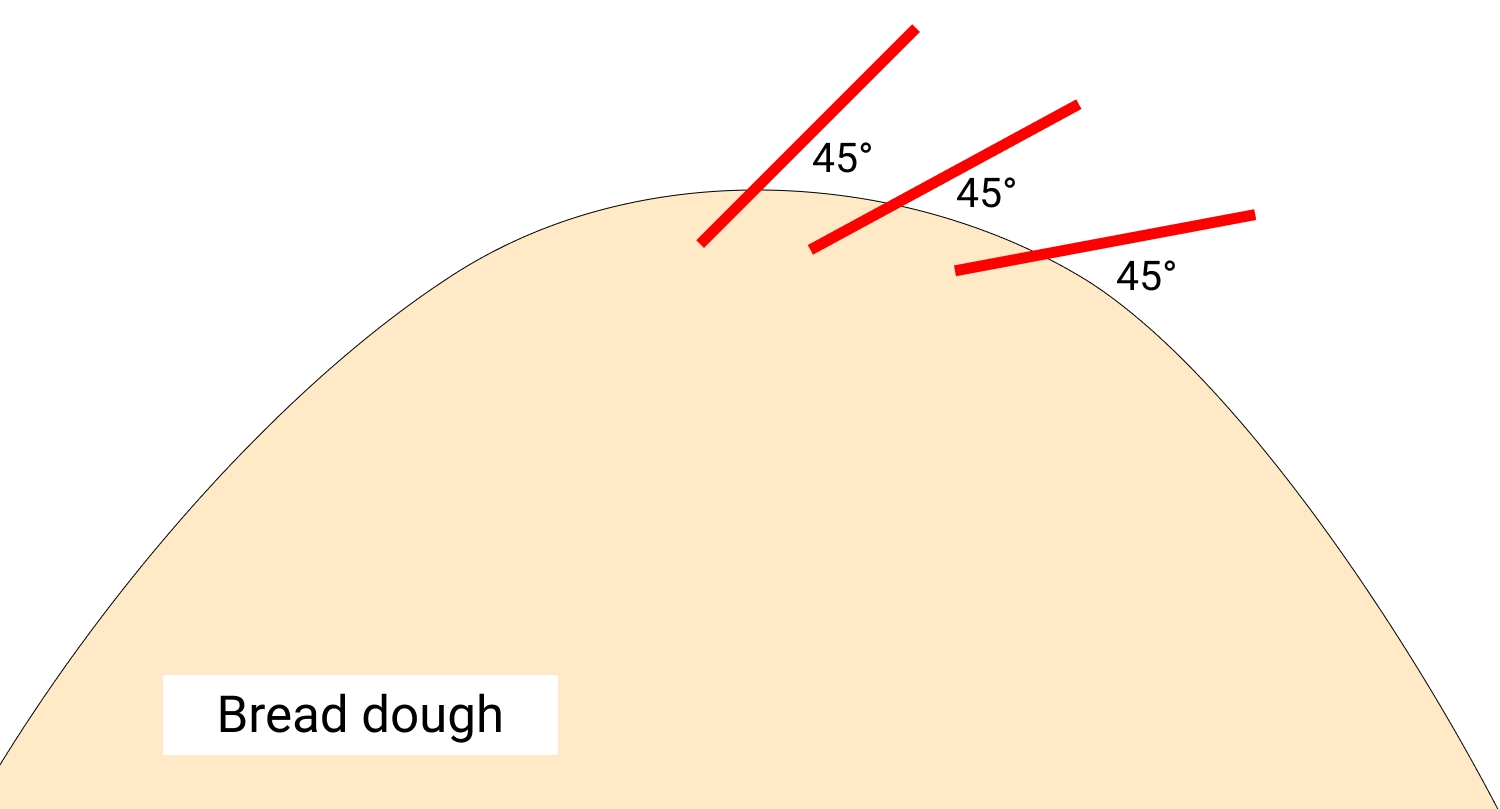
\includegraphics[width=\textwidth]{bread-scoring-angle}
  \caption[Scoring angle]{The \ang{45}~angle at which you score the
      dough is relative to the surface of the dough.  When scoring more towards
      the side, you have to adjust the angle to achieve the ear on your
      bread.}%
  \label{fig:scoring-angle}
\end{figure}

The actual incision is done with a very sharp knife, or better, a razor
blade. You can use the razor blade directly or attach it to a chopstick.
The razor blade offers better flexibility than the sharp knife.
Regardless, the blade should be as sharp as possible. This way when cutting,
the dough is not torn and instead features a clean, non ragged incision.

To simplify scoring, your dough's surface must be dried out a little bit.
This way it is a lot easier to make the incision.
For this reason, it is crucial to rub your dough with a bit of flour
before placing it in the banneton. The dry flour will absorb some of the
moisture of the outer layers of your dough. This is especially important
when working with room temperature-proofed doughs. A cold-proofed dough
is a lot easier to score due to the dough's low viscosity. The room-temperature
dough is a lot harder to score. The scoring incision tears a lot
easier. With a ragged incision, the dough is not as likely to properly
rise in the oven. Chances are you will not achieve the previously mentioned
ear. For this reason, drying out the surface is especially important. Scoring
will become a lot easier.

\begin{figure}[htb!]
  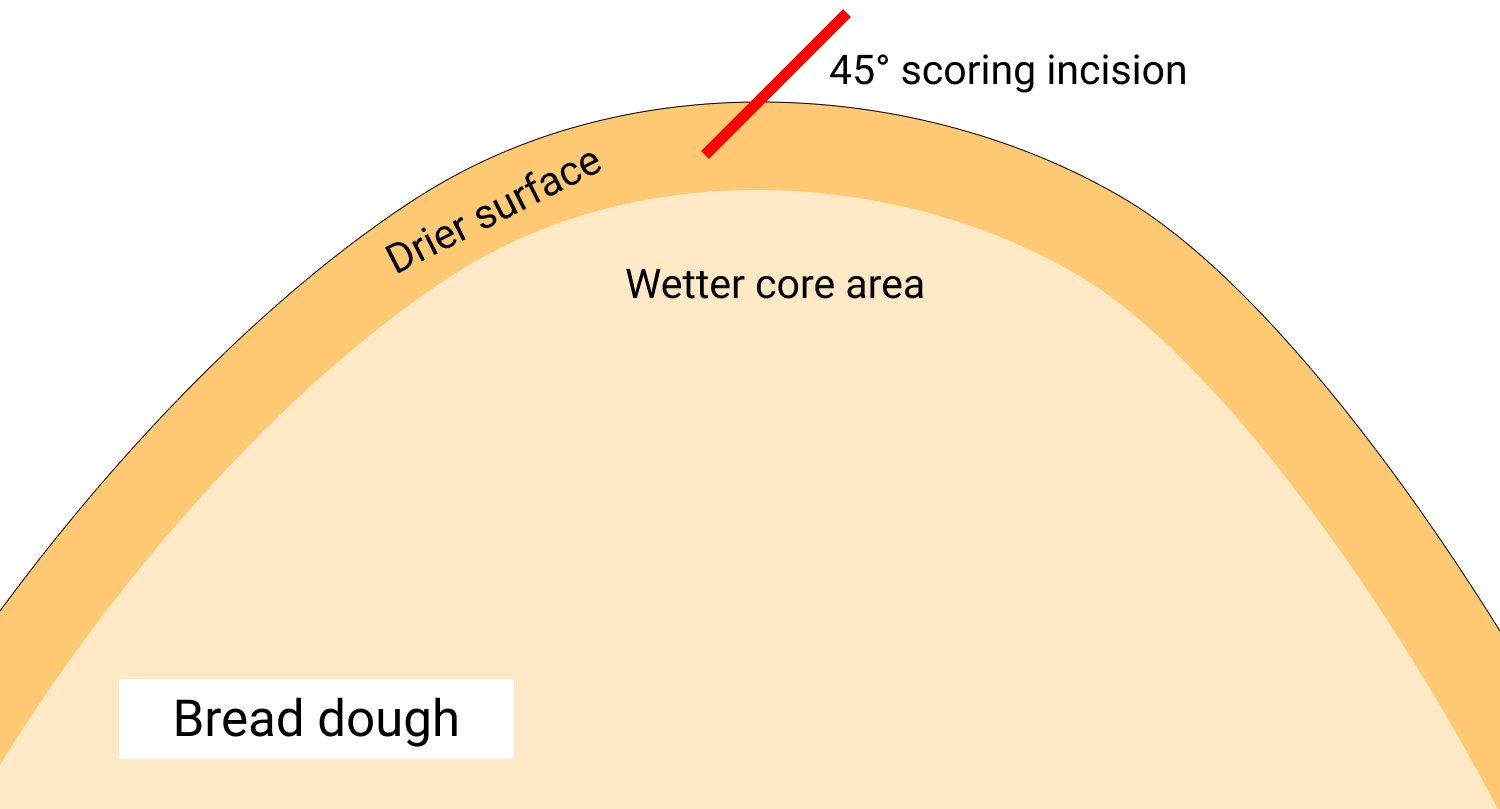
\includegraphics[width=\textwidth]{dry-dough-surface}
  \caption[Drying the dough surface]{By applying flour to your dough's surface
      after shaping, the outer part of the dough dries out a little bit. This
      makes scoring a lot easier as the incision is less likely to tear.}%
  \label{fig:dried-out-dough-scoring}
\end{figure}


Scoring requires a lot of practice. For this reason, I~recommend
practicing making the incision after creating dough strength. The dough
is going to be very wet and sticky. You can use a sharp knife or razor
blade to practice the technique. Wait a few minutes and then round
up the dough again. You can practice this for as long as you like
until you are happy with your technique. After proofing, you only
have a single chance to practice scoring. It's either hit or miss.

An additional trick that can help you to combine the benefits
of room temperature-proofing and easy cold-proofing scoring
is to place your dough in the freezer for 30~minutes before baking.
Once you notice your dough is almost done proofing, move it to the
freezer. The freezer will dry out the dough's surface even further
while also lowering its viscosity, making scoring easier.

Another interesting trick is to bake your dough for 30 seconds without steam.
The hot air will dry out the dough's surface even further and simplify
the scoring technique. Experiment with the timing to identify your personal
sweet spot.


\chapter{Non wheat sourdough}%
\label{chapter:non-wheat-sourdough}
\begin{figure}[!htb]
  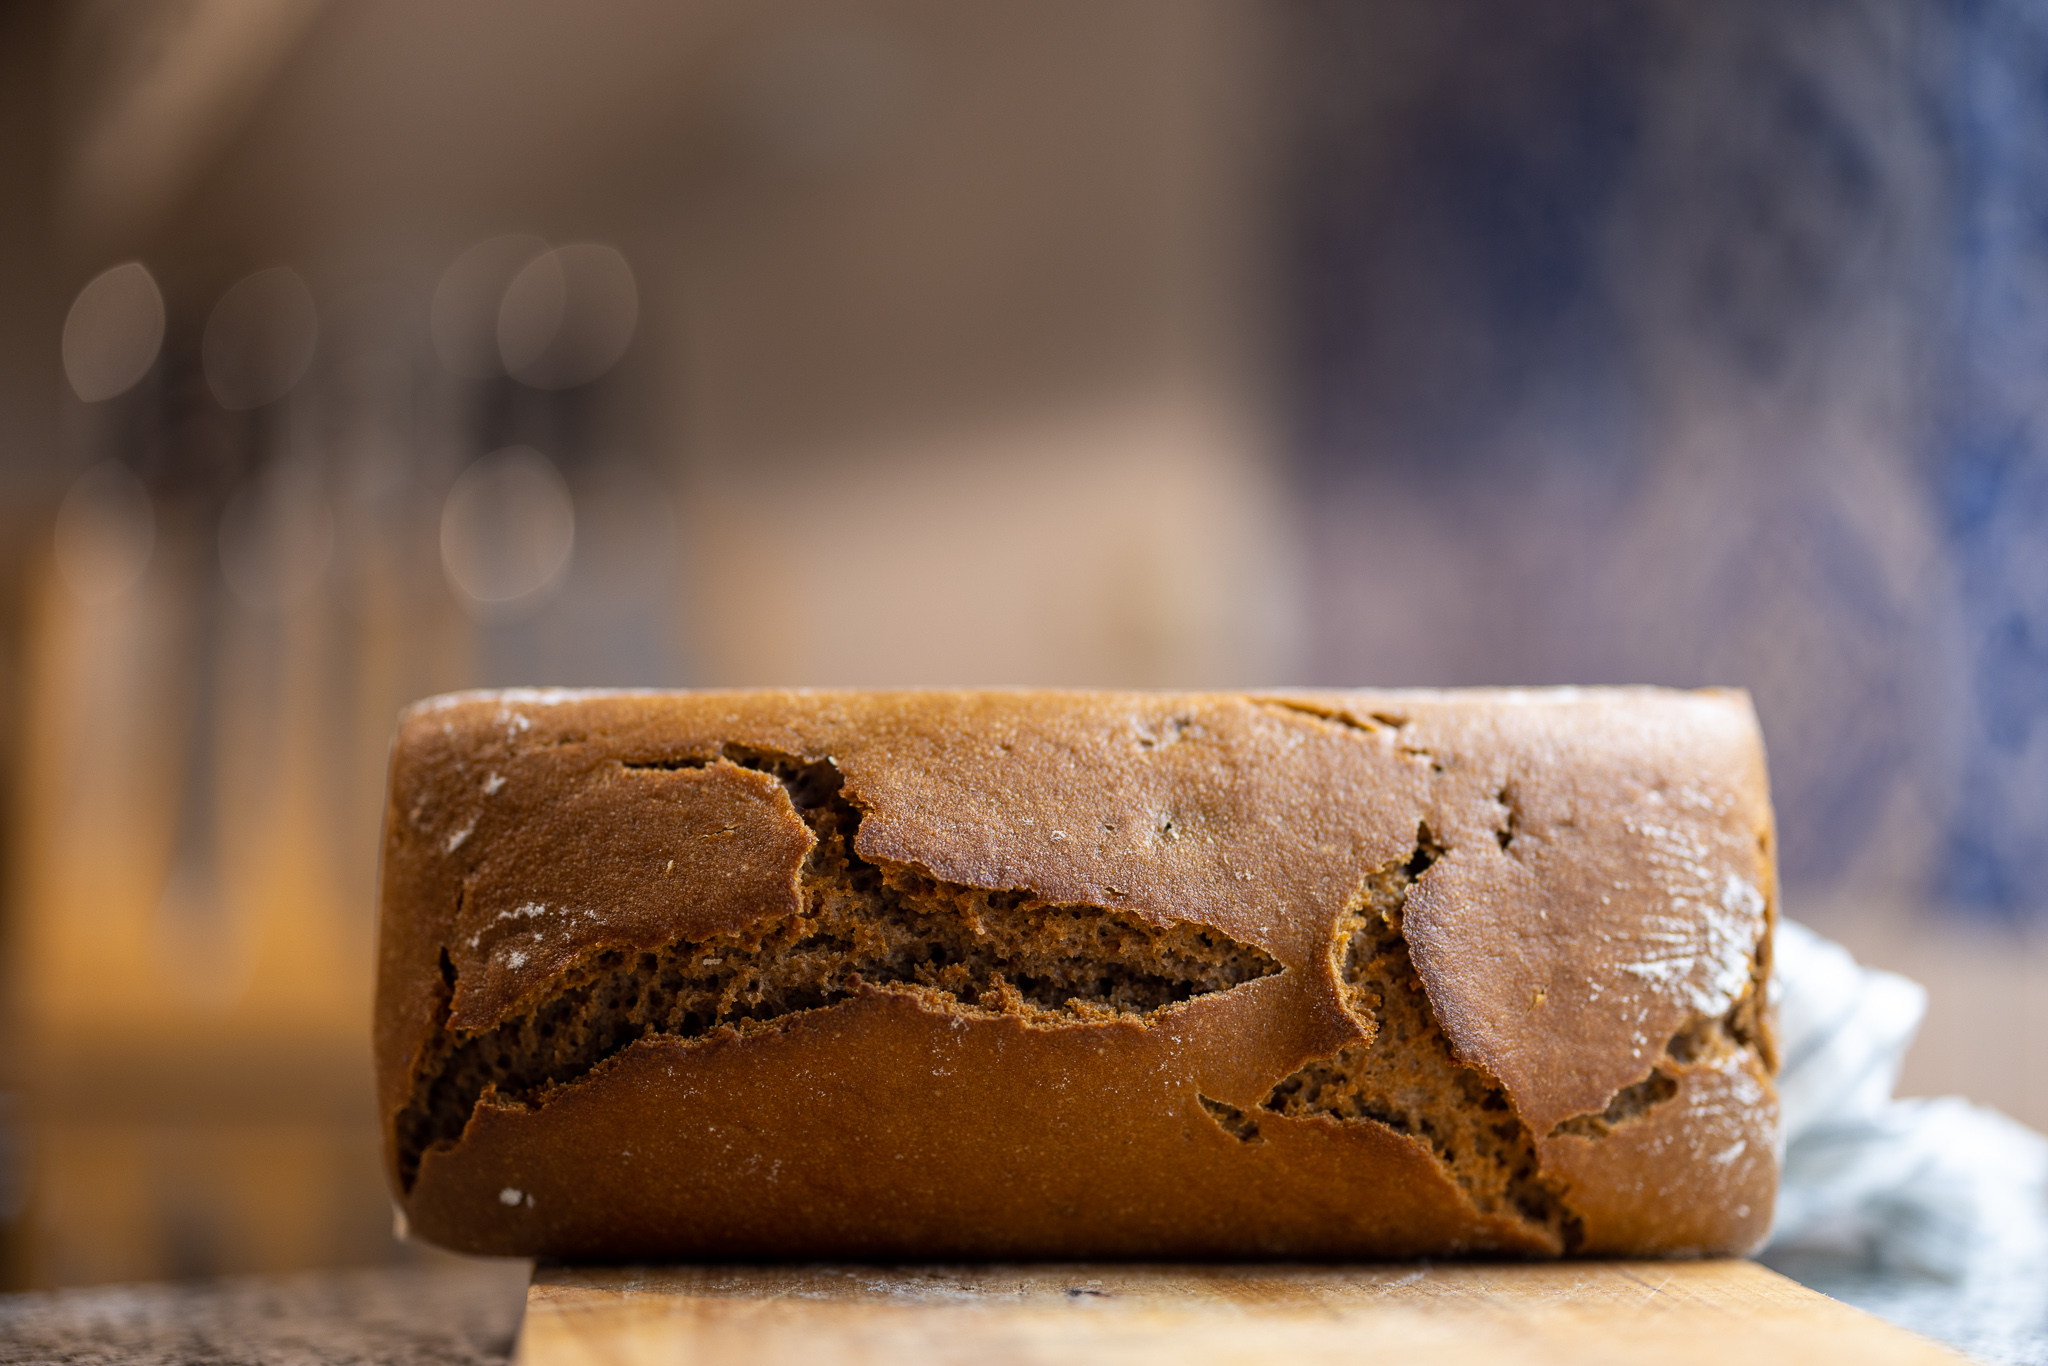
\includegraphics[width=\textwidth]{final-bread}
  \caption{A sourdough rye bread made using a loaf pan. The
  rye bread is not scored. The crust typically cracks
  open during baking.}
  \label{fig:non-wheat-final-bread}
\end{figure}

In this chapter you will learn how to make a basic sourdough bread
using non-wheat flour. This includes all flour except spelt.
The key difference between wheat and non-wheat flour is
the quantity of gluten. Wheat and spelt feature a high amount
of gluten. The non-wheat flours do not. In the case of rye flour,
sugars called pentosans prevent gluten bonds from properly
forming~\cite{rye+pentosans}.

For these flours including rye, emmer, and einkorn, no gluten
development has to be done. This means there is no kneading,
no over-fermentation, and no issues with making flat bread.
The whole process
is a lot easier. You mix the ingredients and
wait for a certain period until the dough has
reached the level of acidity that you like. Afterward, you
shape the dough or pour it into a loaf pan. After a short proofing
period, the bread can be baked. Due to the lack
of gluten development, the final bread will feature a denser
crumb compared to wheat.

\begin{figure}[!htb]
  \includegraphics{figures/fig-non-wheat-process.pdf}
  \caption{A visualization of the process to make non-wheat sourdough bread.
  The process is much simpler than making wheat sourdough bread. There is
  no gluten development. The ingredients are simply mixed together.}
  \label{fig:non-wheat-sourdough}
\end{figure}

This chapter will focus on making rye bread. The flour could
be replaced with einkorn or emmer based on your preference.

The following recipe will make you 2 loaves:
\begin{itemize}
  \item 1000 g of whole rye flour
  \item 800 g of room temperature water (80 percent)
  \item 200 g of sourdough starter (20 percent)
  \item 20 g of salt (2 percent)
\end{itemize}

The sourdough starter can be in an active or inactive state. If it has been
at room temperature for a week with no feedings then it will be okay, or 
if it has come right out of the fridge then still it will be no problem.
The dough is very forgiving.

If you follow the suggested dough from the recipe you are making a relatively
wet rye dough. It's so wet that it can only be made using a loaf pan. If
you want to make a freestanding rye bread, consider reducing the hydration
to around 60 percent.

\begin{figure}[!htb]
  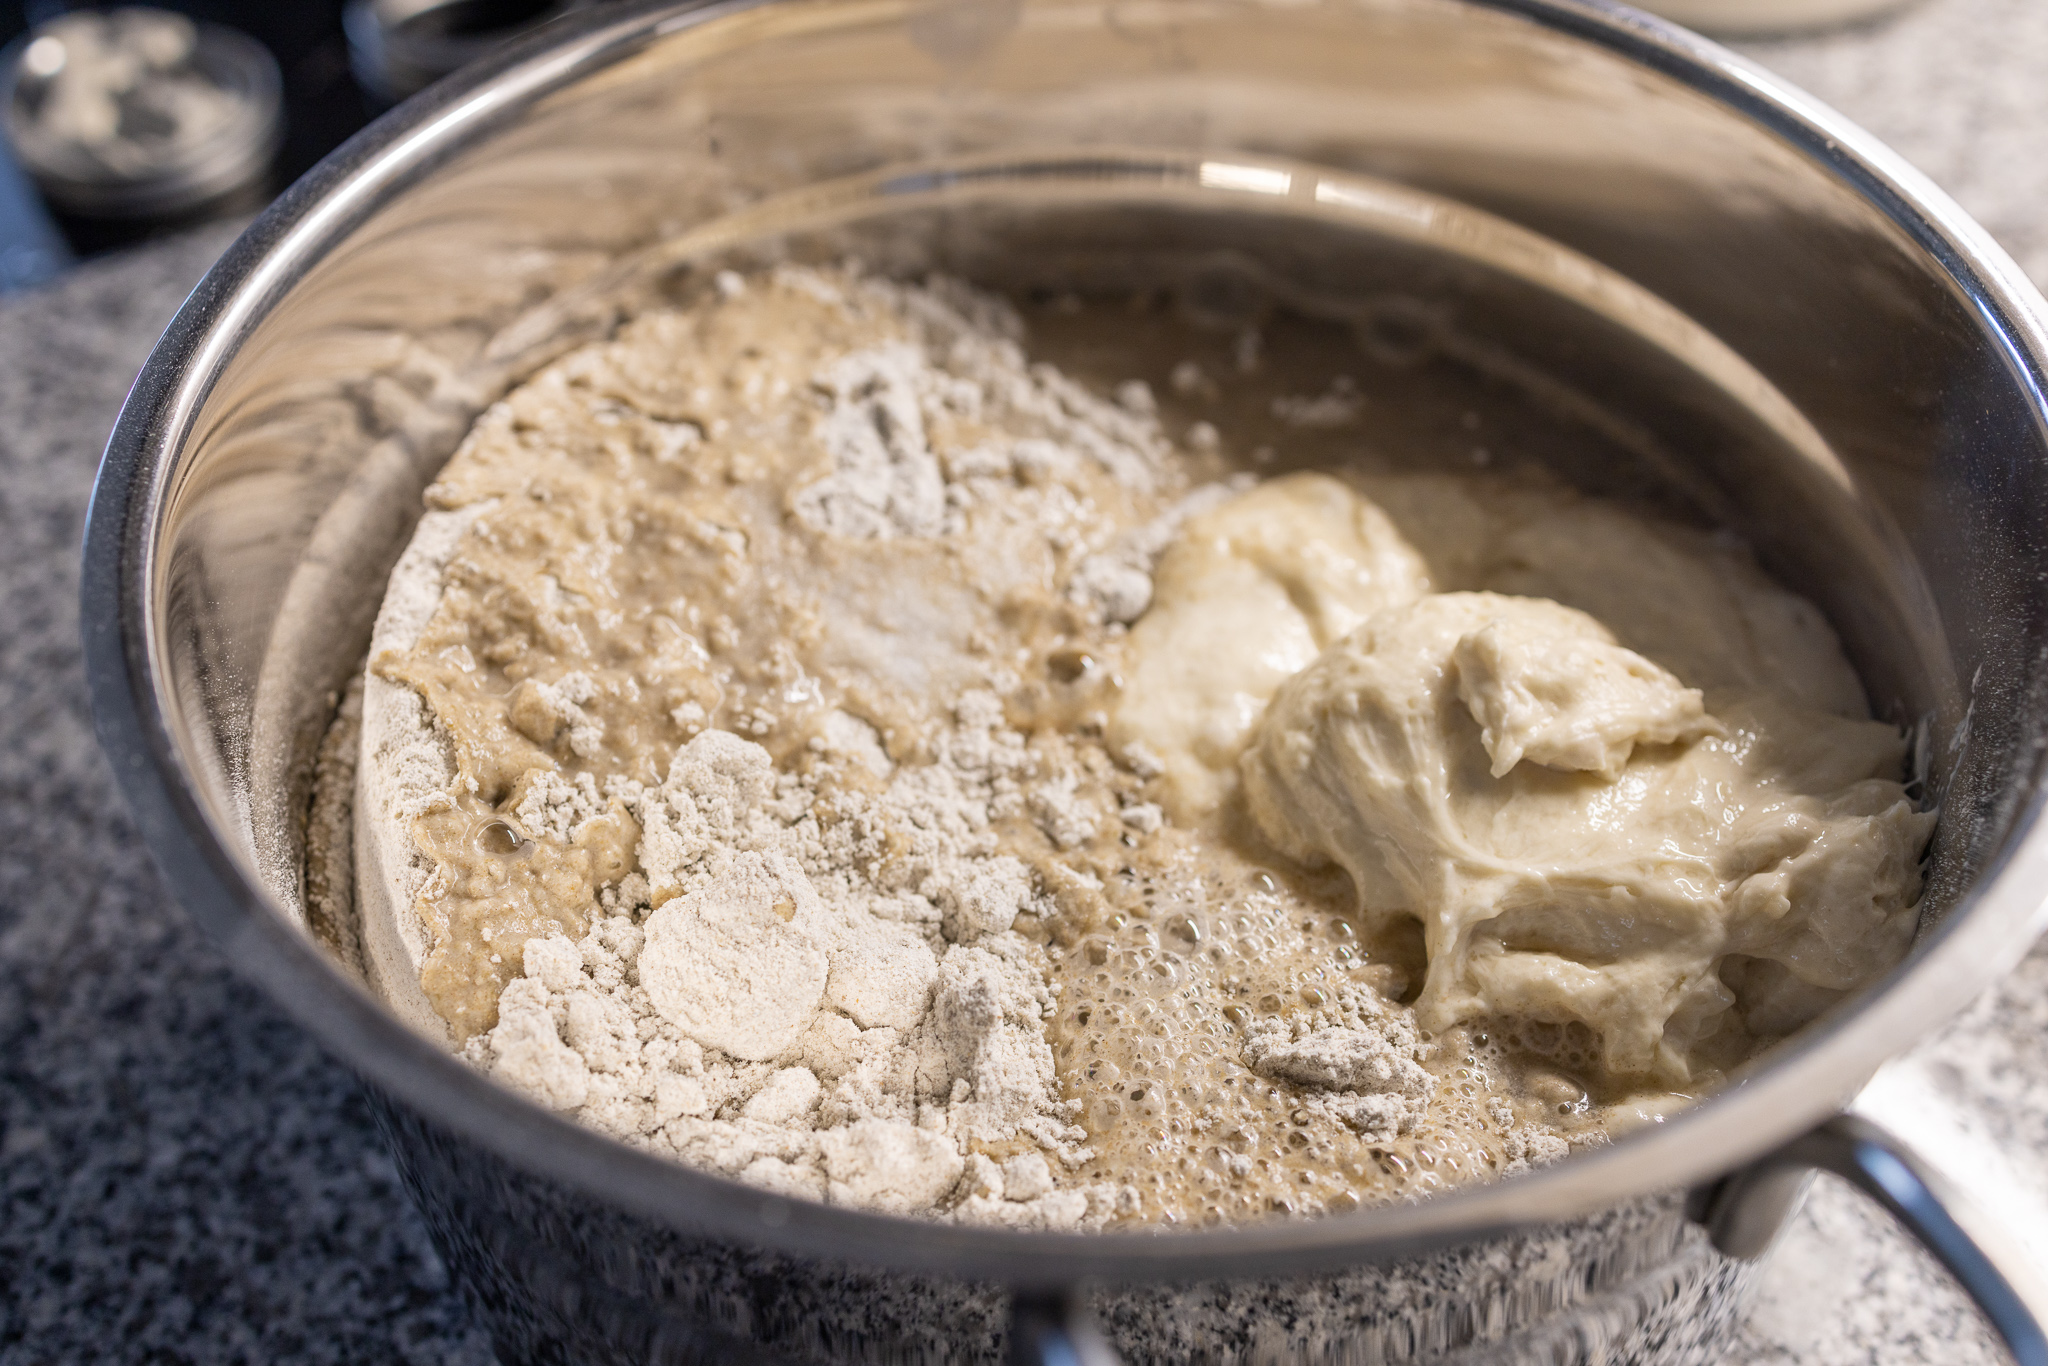
\includegraphics[width=\textwidth]{ingredients}
  \caption{For non-wheat dough the ingredients are mixed together. There is no need
  to develop any dough strength. This simplifies the whole bread-making process.}
  \label{fig:non-wheat-ingredients}
\end{figure}

Mix together all the ingredients with your hands. You can also
opt for a spatula to simplify things. Rye flour itself is very
sticky and unpleasant to mix by hand. The dough will stick
a lot to your hands. If you use a stiff starter, it can be
easier to dissolve it in the dough's water. Once dissolved,
add the other ingredients.

\begin{figure}[!htb]
  \includegraphics[width=\textwidth]{sticky-hands}
  \caption{Rye flour has a sugar molecule known as pentosan. These pentosans prevent
  the rye flour from building gluten bonds. As a result the dough never features an
  open crumb and is always very sticky when hand mixing.}
  \label{fig:non-wheat-sticky-hands}
\end{figure}

The goal of the mixing process is to homogenize the dough. There
is no need to develop any dough strength. Once you see that
your sourdough starter has been properly incorporated, your
dough is ready to begin bulk fermentation.

You can bulk ferment the dough for a few hours up to
weeks. By extending the bulk fermentation time, you increase
the acidity the final loaf is going to feature. After around
48 hours, the acidity will no longer increase. This is because
most of the nutrients have been eaten by your microorganisms.
You could let your dough sit for longer, but it wouldn't alter the
final flavor profile by much.

I~recommend waiting until the dough has roughly increased by
50 percent in size. If you are daring, you can taste the dough
to get an idea of the acidity profile. The dough will likely
taste very sour. However, a lot of the acid will evaporate
during the baking process. So the final loaf will not be
as sour as the dough you are tasting.

Once you are happy with the acidity level, proceed to dividing
and shaping your dough. Shaping might not be possible if you opt
for the wetter dough. If you made a drier dough, use as much
flour as needed to dry the dough a little bit and form a dough ball.
There is no folding the dough. All you do is tuck it together
as much as is needed to apply the shape of your banneton.
For the wetter dough, use a spatula and pour as much dough as
needed into your greased loaf pan.

\begin{figure}[!htb]
  \includegraphics[width=\textwidth]{crumb}
  \caption{The crumb structure of rye bread. By making a wetter
  dough, more water evaporates during the baking and thus the
  crumb tends to be a bit more open. Generally, rye
  bread is never as fluffy as wheat sourdough bread. The crust
  of this bread is a bit pale. The crust color can be controlled
  by baking the bread for a longer period.}
  \label{fig:rye-crumb}
\end{figure}

Carefully spread the dough with a spatula in your loaf pan. You
can wet the spatula to make this process easier. Spread it
until the surface looks smooth and shiny.

For proofing, I~recommend waiting around 60 minutes. An extended
proofing period does not make sense unless you want to further
increase the dough's acidity. The dough will not become fluffier
the longer you proof. With the short proofing period, however,
the dough will become a bit more homogenous. This way the final
bread looks more uniform. The proofing period also allows the
dough to fully extend and fill the edges of the loaf pan. I~also
like to move the dough to the fridge for proofing. The dough stays
good in the fridge for weeks. You can proceed and bake it at a
convenient time for you. 

Once you are happy with the proofing stage, proceed and bake your dough
just like you'd normally do. For more details please refer to 
Chapter~\ref{chapter:baking}. One challenging aspect
of using a loaf pan is to make sure that the center part of your
dough is properly cooked. For this reason, it is best to use a thermometer
and measure the internal temperature. The bread is
ready once the internal temperature reaches 92°C (197°F). I~recommend
removing the bread from the loaf pan once it reaches the desired
temperature. Then you can continue baking the loaf without the pan and
steam. This way you achieve a great crust all around your
loaf. You can bake as long as you like until you have achieved
your crust color of choice. The darker, the more crunchy
the crust and the more flavor it offers. If you feel your
dough might have been overly acidic, you can extend the baking time.
The longer you bake, the more acidity will evaporate.

This is one of my favorite breads to bake which I~eat on an
almost daily basis. The effort required to make bread like
this is much lower compared to a wheat-based dough. In some
cases, I~extend the recipe and add additional sourdough discard
to the dough. You can add as much discard as you like. The resulting
bread has a very complex but delicious flavor profile.


\chapter{Baking}%
\label{chapter:baking}
\chapter{Baking}%
\label{chapter:baking}
\begin{quoting}
Baking refers to the part of the process where you are loading your dough into
the oven\footnote{While some breads like flatbreads could also be baked on the
stove. This chapter focuses on the home oven.}.  Baking is typically done after
your dough has gone through the bulk fermentation and proofing stage.  This
chapter will review what happens to your dough during baking, as well as
several techniques used to improve the final result.
\end{quoting}

\section{The process of baking}
Once temperature starts to rise, the dough will go through several stages as
summarized in Table~\ref{tab:baking-stages}.  As the dough heats up, the water
and acids in your dough start to evaporate. When baking a gluten based dough,
the bubbles in your dough start to expand.  The dough starts to vertically
rise, this is called oven spring.  Your bread starts to build a crust of
gel-like consistency, the crust is still extensible and can be stretched.

\begin{table}[htp!]
    \begin{center}
        \begin{tabular}{@{}rlp{0.5\textwidth}@{}}
\toprule
\thead{°C / °F} & \thead{Stage}           & \thead{Description} \\ \midrule
60 / 140        & Sterilization           & The temperature is too hot for your microorganisms and they die.\\ 
75 / 167        & Gel building            & A gel builds on the surface persisting your dough's structure.
                                            It is still extensible and can spring in the oven.\\ 
100 / 212       & Water evaporation       & Water begins to evaporate and inflates your dough's alveoli.\\ 
118 / 244       & Acetic acid evaporation & The vinegary tasting acid starts to evaporate, sourness decreases.\\ 
122 / 252       & Lactic acid evaporation & The dairy tasting lactic acid begins to evaporate, sourness further decreases.\\ 
140 / 284       & Maillard reaction       & The Maillard reaction starts to deform starches and proteins. 
                                            The dough starts browning.\\ 
170 / 338       & Caramelization          & Remaining sugars begin to caramelize giving your bread a distinct flavor.\\ \bottomrule
\end{tabular}

        \caption[Stages of dough during baking]{The different stages that
            your dough undergoes during the baking process.}%
        \label{tab:baking-stages}
    \end{center}
\end{table}

At around  \qty{60}{\degreeCelsius} (\qty{140}{\degF}) the microbes in your dough start to die.
There are rumors that until this happens the microbes produce
a lot of \ch{CO2}, resulting in the dough's expansion. However, this temperature
is reached quickly. Furthermore, stress makes the microbes
enter sporulation mode in order to focus on spreading genetics.
More research should be done here to validate or invalidate this
claim.

At  \qty{75}{\degreeCelsius} (\qty{167}{\degF}) the surface of your dough turns into a gel. It
holds together nicely but is still extensible. This gel is essential
for oven spring as it retains the gas inside your dough.

At around  \qty{100}{\degreeCelsius} (\qty{212}{\degF}) the water starts to evaporate out of your
dough. If this weren't the case, your dough would taste soggy and
doughy. The higher hydration your dough has, the more water your bread
still contains after the bake, changing its consistency.  As a result the
crumb is going to taste a bit more moist.

Another often undervalued step is the evaporation of acids.
At~\qty{118}{\degreeCelsius} (\qty{244}{\degF}) the acetic acid in your dough
starts to evaporate.
Shortly after at~\qty{122}{\degreeCelsius} (\qty{252}{\degF}) the lactic acid begins evaporating.
This is crucial to understand and it opens the door to many interesting
ways to influence your final bread's taste. As more and more water
begins to evaporate the acids in your dough become more concentrated.
There is less water but in relation you have more acids, therefore a shorter
bake will lead to a more tangy dough. The longer you bake the bread,
the more of the water evaporates, but also ultimately the acids will follow.
The longer you bake, the less sour your bread is going to be. By controlling
baking time you can influence which sourness level you would like to achieve.

It would be a very interesting experiment to bake a bread at different exact
temperatures. How would a bread taste with only evaporated water but
full acidity? What if you were to just completely get rid of the acetic
acid? How would the taste change?

\begin{figure}[!htb]
  \includegraphics[width=\textwidth]{baking-experiment-temperatures.png}
  \caption[Surface temperature for different steaming methods]{This
      chart shows how surface temperatures change using different steaming
      methods. In this case I~used a Dutch oven and an apple as dough
      replacement. All the apples were coming from the fridge. The temperature
      was measured using a barbecue thermometer.  The more steam, the faster
      the surface temperature increases.}
\end{figure}

As the temperature increases further the crust thickens. The Maillard reaction
kicks in, deforming proteins and starches. The outside of your dough starts to
become browner and crisper, this process begins at
around~\qty{140}{\degreeCelsius} (\qty{284}{\degF})

Once the temperature increases even more to around~\qty{170}{\degreeCelsius}
(\qty{338}{\degF}),
the caramelization process begins, the remaining sugars and the microbes which
did not convert yet start to brown and darken. You can keep baking
for as long as you like to achieve the crust color that you
like\footnote{This really depends a lot on your personal preference.
Some people prefer a darker crust, others prefer a more pale crust.
It's better to build less crust than too much. You can always just
heat your bread in the oven one more time to continue building a
darker crust.}.

The best method to know that your dough is done is to take
the temperature of your dough, you can use a barbecue thermometer
to measure it. Once the core temperature is at around~\qty{92}{\degreeCelsius}
(\qty{197}{\degF}),
you can stop the baking process. This is typically not done though
as the crust hasn't been built yet\footnote{The thermometer is
especially important when using a large loaf pan. It is sometimes
very hard to judge from the outside if the dough is done. I~failed
many times and ended up having a semi baked dough.}.

Once your dough has finished baking, it is ready to eat: your
dough has turned into a bread. At this
point, your bread is sterile as the temperature was too hot for
for the microorganisms to survive\footnote{I~wonder though
if a starter culture could be grown again from a slice of bread.
Under heat stress the microorganisms begin sporulating. Maybe
some of the spores survive the baking process and could be reactivated
later? If this works, you could use any store bought sourdough
bread as a source for a new starter.}.

\section{The role of steam}
Steam is essential when baking as it helps to counter premature
crust building. During the first stage of the bake, the dough
increases in size as the water in your dough evaporates and pushes
the whole dough upwards.

Normally, under high heat a crust would form. Just like
if you were to bake vegetables in your home oven, at some point
they become darker and crisper. This is the same thing that
happens with your dough, and you want to delay this process
as long as possible until your dough no longer expands.
Expansion stops when most of the microbes have died and
the evaporating water no longer stays inside the alveoli.

The stronger the gluten network, the more gas can be retained
during the baking process. This gluten network at some point
loses its ability to contain gas as the temperature heats
up. The dough stops increasing in size. The steam plays
an important role as it condenses and evaporates on top
of your dough. The surface temperature is rapidly increasing
to around~\qty{75}{\degreeCelsius} (\qty{160}{\degF}). At this temperature the
gel starts to build, and is still extensible and allows expansion.
Without the steam, the dough would never enter the gel stage,
but instead directly go to the Maillard reaction zone. You
want your dough to stay in this gel stage as long as possible
to achieve maximum expansion\footnote{You can remove your
dough from the oven after 5~minutes to see the gel. You will notice
that it holds the dough's structure and it has a very interesting consistency.}.

\begin{figure}[!htb]
  \includegraphics[width=\textwidth]{baking-process-stage-2.jpg}
  \caption[Baking step~2, without steam]{The second stage of the bake is done
      without steam to build a thicker, darker crust.}
\end{figure}

When not steaming enough, you will notice that the scoring
incisions do not properly open up during the bake. They stay
closed as the dough is unable to push through the crust.
Another common sign, as you can see in Figure~\ref{fig:too-little-steam} is
that you have larger pockets of air towards the crust of your dough. As the
dough increases vertically, expansion is halted by the crust. The pockets
of air converge into larger pockets as the pressure increases.
This can also happen when you are baking at too high a temperature.

The more you steam, the softer your dough's crust is. You will never
enter the Maillard and caramelization stage. This
is the reason why the source of steam is removed
for the second stage of the bake. No more expansion can
happen and you can focus on building a crust. If you
would like a soft crust, you can steam your dough all the
way.

\begin{figure}[!htb]
  \includegraphics[width=\textwidth]{baking-too-hot}
  \caption[Bread baked too hot]{A submission by Karomizu showing a bread that
      has been baked at too high a temperature or with too little steam. Note
      the large pockets of air towards the crust. They are a typical
      indicator.}%
      \label{fig:too-little-steam}
\end{figure}

\section{Building up steam}
\begin{flowchart}[!htb]
\begin{center}
  \begin{tikzpicture}[node distance = 3cm, auto]
  \node [block] (heat_oven) {\footnotesize Heat oven to 230°C (446°F) for 30 minutes};
  \node [block, right of=heat_oven, node distance=3cm] (score_dough) {\footnotesize Score your dough};
  \node [decision, right of=score_dough, node distance=4cm] (decide_steam) {\footnotesize Choose your steaming method};
  \node [block, below of=heat_oven, node distance=4cm] (inverted_tray_method) {\footnotesize Inverted tray method};
  \node [block, right of=inverted_tray_method, node distance=3cm] (dutch_oven) {\footnotesize Dutch oven};
  \node [block, right of=dutch_oven, node distance=3cm] (steam_injection) {\footnotesize Steam injection oven};
  \node [block, below of=inverted_tray_method, node distance=3cm] (bake_30) {\footnotesize Bake dough for 30 minutes with steam};
  \node [block, right of=bake_30, node distance=3cm] (remove_steam) {\footnotesize Remove source of steam};
  \node [block, right of=remove_steam, node distance=3cm] (build_crust) {\footnotesize Build the crust};
  \node [block, right of=build_crust, node distance=3cm] (finish_baking) {\footnotesize Stop baking 10--30 minutes later depending on crust preference};
  \path [line] (heat_oven) -- (score_dough);
  \path [line] (score_dough) -- (decide_steam);
  \path [line] (decide_steam) -- (inverted_tray_method);
  \path [line] (decide_steam) -- (dutch_oven);
  \path [line] (decide_steam) -- (steam_injection);
  \path [line] (steam_injection) -- (bake_30);
  \path [line] (inverted_tray_method) -- (bake_30);
  \path [line] (dutch_oven) -- (bake_30);
  \path [line] (bake_30) -- (remove_steam);
  \path [line] (remove_steam) -- (build_crust);
  \path [line] (build_crust) -- (finish_baking);
\end{tikzpicture}

  \caption[Different steaming methods]{A schematic visualization of the baking
      process using different sources of steam in a home oven.}%
  \label{fig:baking-process}
\end{center}
\end{flowchart}

\begin{figure}[!htb]
  \includegraphics[width=\textwidth]{oven-example}
  \caption[Home oven baking example to maximize steam]{My default home oven setup. The tray of rocks
  and tray on top of the rolls greatly improve the steaming capabilities. This way the bread can
  rise more during the initial stage of the baking process.}
\end{figure}

\begin{figure}[!htb]
  \includegraphics[width=\textwidth]{baking-process-steam.jpg}
  \caption[Steam building with inverted tray]{How steam builds in your oven
      using the later described inverted tray method.}%
      \label{flc:inverted-tray}
\end{figure}

\subsection{Dutch ovens}

\begin{figure}[!htb]
  \includegraphics[width=\textwidth]{dutch-oven-example}
  \caption[Picture of dutch oven]{An example of a dutch oven. Some are also
      made out of enameled cast iron, others are made out of clay and some
      feature a glass lid.  They all work similarly by entrapping some of the
      steam created during the baking process. The steamy environment allows
      the bread to rise further and thus have more oven spring and feature a
      fluffier crumb.}%
\end{figure}

\begin{flowchart}[!htb]
\begin{center}
  \begin{tikzpicture}[node distance = 3cm, auto]
  \node [start] (heat_oven) {Preheat DO to \qty{230}{\degreeCelsius} (\qty{446}{\degF}) for 30~minutes};
  \node [block, right of=heat_oven] (remove_oven) {Remove DO from oven };
  \node [block, right of=remove_oven] (open_load_dough) {Open DO \& load your dough};
  \node [block, right of=open_load_dough] (score) {Score your dough};
  \node [block, right of=score] (spritz) {Spritz dough with water};
  \node [block, below of=spritz] (close) {Close DO};
  \node [block, left of=close] (back_oven) {Place DO back in oven};
  \node [block, left of=back_oven] (bake) {Bake 30~minutes at \qty{230}{\degreeCelsius} (\qty{446}{\degF})};
  \node [decision, below right= 5cm and -1 cm of heat_oven]  (is_ready_check)
        {Core temperature \qty{92}{\degreeCelsius} (\qty{197}{\degF})?};
  \node [block, below of=is_ready_check, node distance=4cm] (wait_5_minutes) {Wait\\ 5 minutes};
  \node [block, right of=is_ready_check, node distance=4cm] (remove_do_lid) {Remove DO lid};
  \node [decision, right of=remove_do_lid, node distance=3.5cm] (dark_enough_decision) {Crust color dark enough?};
  \node [success, below of=dark_enough_decision, node distance=4cm] (finish_baking) {Bread is finished};
  \node [block, right of=dark_enough_decision, node distance=3.5cm] (bake_5_more_minutes) {Bake another 5~minutes};
  \path [line] (heat_oven) -- (remove_oven);
  \path [line] (remove_oven) -- (open_load_dough);
  \path [line] (open_load_dough) -- (score);
  \path [line] (score) -- (spritz);
  \path [line] (spritz) -- (close);
  \path [line] (close) -- (back_oven);
  \path [line] (back_oven) -- (bake);
  \path [line] (bake.west) -- node{} ++(-2, 0) -| (is_ready_check.north);
  \path [line] (is_ready_check) -- node{yes} (remove_do_lid);
  \path [line] (is_ready_check) -- node{no} (wait_5_minutes);
  \path [line] (wait_5_minutes.west) -- node{} ++(-1.5, 0) |- (is_ready_check.west);
  \path [line] (remove_do_lid) -- (dark_enough_decision);
  \path [line] (dark_enough_decision) -- node{yes} (finish_baking);
  \path [line] (dark_enough_decision) -- node{no} (bake_5_more_minutes);
  \path [line] (bake_5_more_minutes.east) -- node{} ++(1, 0) -- node{} ++(0, 2.3) -| (dark_enough_decision.north);
\end{tikzpicture}

  \caption[Baking process with a dutch oven]{A visualization of the baking
      process using a dutch oven (DO). The dough is steamed for the first half
      of the bake and then baked without cover for the second half of the
      bake. The desired darkness and thickness of the crust depends on your
      personal preference. Some bakers prefer a lighter crust and others a
      darker.}%
  \label{fig:dutch-oven-process}
\end{center}
\end{flowchart}

Dutch ovens are an ideal way to bake with a lot of
steam. They are not fully sealed. Regardless though,
as water evaporates from your dough, it will create a steamy
environment allowing your dough to rise. It
makes baking in a home oven very easy.

When using a Dutch oven, make sure to preheat it properly,
this way your dough will not stick to it. You can also
use additional semolina flour or parchment paper. Another
good trick is to spritz your dough with a bit of water.
To create more steam, you could also place a small ice cube
next to your main dough.

I~have been using a Dutch oven myself for a long time. They
have issues though. They are relatively heavy. It is dangerous
to operate hot cast iron ovens. Especially when working with steam,
you have to be very careful. Furthermore,
they are expensive to buy. If your Dutch oven is made out
of cast iron you have to season it from time to time. This takes
time.

The biggest disadvantage, though, is
capacity. You can only bake a single piece of bread at a time,
as the size of the Dutch oven is limited.
In many cases, it makes sense to bake multiple
loaves in one go. It makes the whole process more
efficient as you have to knead less per loaf. The time it
takes to make one loaf is significantly reduced. Furthermore,
you don't require as much energy. You don't have
to preheat your oven twice for each loaf.

An additional disadvantage of Dutch ovens is the
need to move very hot and heavy cast iron\footnote{%
  Some of them can weigh up to 10 kg. Moving them is quite
  a tedious exercise. Especially if the cast iron is
  heated you have to be very concise with your movements.
  Despite doing my best I have a few scars on my
  hands and arms from operating the Dutch ovens.
}.
You will need to be very careful and ideally use
heat-resilient gloves when touching your Dutch oven.

Furthermore, some of the Dutch ovens come at a hefty
price tag. Especially for new bakers buying a Dutch oven on
top of other tools can be quite a hefty investment. For
this reason, I advocate the inverted tray method visualized
in the next section. In case you do not own an oven consider trying
the simple flatbread recipe which is baked in a pan. Please
refer to Section~\ref{section:flat-bread-recipe} for more details.


\subsection{Inverted tray method}

The inverted tray method simulates a Dutch oven.
By placing another tray on top of your dough, the steam
created from the dough and water source stays
around your dough.

\begin{flowchart}[!htb]
\begin{center}
  \begin{tikzpicture}[node distance = 3cm, auto]
  \node [block] (init) {\footnotesize Place water tray and stone in oven};
  \node [block, right of=init] (heat_oven) {\footnotesize Heat oven to  \qty{230}{\degreeCelsius} (\qty{446}{\degF}) for 30~minutes};
  \node [block, right of=heat_oven] (score_your_dough) {\footnotesize Score your dough};
  \node [block, right of=score_your_dough] (spritz) {\footnotesize Spritz your dough with water};
  \node [block, right of=spritz] (load_tray) {\footnotesize Place non-preheated inverted tray in oven};
  \node [block, below of=load_tray, node distance=4cm] (load_doughs) {\footnotesize Load doughs into oven};
  \node [block, left of=load_doughs, node distance=3cm] (load_water) {\footnotesize Place water in heated water tray};
  \node [block, left of=load_water, node distance=3cm] (bake) {\footnotesize Bake 30~minutes or until core temperature is  \qty{92}{\degreeCelsius} (\qty{197}{\degF})};
  \node [block, left of=bake, node distance=3cm] (remove_steam) {\footnotesize Remove steam source and top tray};
  \node [block, left of=remove_steam, node distance=3cm] (finish) {\footnotesize Bake at least another 10~minutes or until crust has your desired color};
  \path [line] (init) -- (heat_oven);
  \path [line] (heat_oven) -- (score_your_dough);
  \path [line] (score_your_dough) -- (spritz);
  \path [line] (spritz) -- (load_tray);
  \path [line] (load_tray) -- (load_doughs);
  \path [line] (load_doughs) -- (load_water);
  \path [line] (load_water) -- (bake);
  \path [line] (bake) -- (remove_steam);
  \path [line] (remove_steam) -- (finish);
\end{tikzpicture}

  \caption[Inverted tray baking process]{A schematic visualization the
  inverted tray baking method that works great for home ovens.}%
  \label{fig:inverted-tray-process}
\end{center}
\end{flowchart}


The biggest advantage of this method compared to the
Dutch oven is scalability. You can bake multiple loaves
at the same time. In my case that is around 2 freestanding
loaves and 4 loaves in a loaf pan.

For the inverted tray you will need the following tools:
\begin{itemize}
\item 2 trays
\item 1 heat resistant bowl
\item Boiling water
\item Oven gloves
\item (Optional) Parchment paper
\end{itemize}

\begin{figure}[!htb]
  \includegraphics[width=\textwidth]{baking-example.jpg}
  \caption{My home oven setup.}
\end{figure}

These are the steps to follow with the inverted tray method:
\begin{enumerate}
\item Preheat the oven to around  \qty{230}{\degreeCelsius} (\qty{446}{\degF}) and
preheat one of the trays.
\item Bring water to boil.
\item Place your loaves on a piece of parchment paper. You
can also place each on a tiny piece of parchment paper.
This makes loading the dough easier. If you don't
have it or don't want to use it, you can opt for
semolina flour. It helps to make the tray nonstick.
\item Take out your hot tray and place it
on a cooling rack or on something else that
is heat resistant.
\item Score your doughs.
\item Place your doughs on the hot tray.
\item Place the cold tray in your oven in an inverted position.
\item Move your hot tray including the loaves back
to the oven.
\item Place the boiling water in the heat-resistant
water bowl. I~have added rocks to it, as it helps
to improve the steam even further. This is optional.
\item Close the oven.
\item After 30~minutes remove the top tray. Also remove the bowl with water.
\item Finish baking your bread until you have reached your desired
crust color. In my case this is another 15--25~minutes typically.
\end{enumerate}

\section{Conclusions}

\begin{table}[!htb]
    \begin{center}
        % TODO: Not great Looking... 
\begin{tabular}{@{}p{0.25\textwidth}ccc@{}}
\toprule
\thead{Oven type}  & \thead{Plain (no tools)} & \thead{Inverted tray} & \thead{Dutch oven} \\ \midrule
Gas                & No                       & No                    & Yes                 \\ \midrule
Convection (Fan always on) & No               & No                    & Yes                 \\ \midrule
Convection (Fan can be disabled) & No         & Yes                   & Yes                 \\ \midrule
Steam              & Yes                      & Yes                   & Yes                 \\
\bottomrule
\end{tabular}

        \caption[Different oven types]{An overview of different oven types and their
            different baking methods.}
    \end{center}
\end{table}

Depending on your home oven, a different method
of steaming may be used. Generally most ovens
are made to vent out most of the steam during the
bake. They are typically not fully closed. During
baking you want to dry out whatever you are baking.
This is ideal if you are roasting vegetables and
want them to dry out. For baking though, this is
highly problematic. As described earlier, you
want there to be as much steam as possible.

If you are using a gas-based oven, the only option
is to utilize a Dutch oven. The same is true when you
are using a convection oven with a fan that
cannot be disabled. When using a convection
oven with a fan that can be turned off, you can
opt to use the cost-efficient inverted tray
method.

If you are in the luxurious
position of owning a steam oven, things are easier.
Just activate the steam function and you are
good to go. Placing an additional tray on top of your
dough during the bake helps to bake with indirect
heat. You remain in the gel zone longer and
will experience more oven spring.


\chapter{Storing bread}%
\label{chapter:storing-bread}
\begin{quoting}
In this chapter you will learn about different
methods of storing your bread. This way
your bread can be best enjoyed at a later
time.
\end{quoting}

\begin{table}[!htb]
    \begin{center}
        \begin{tabular}{@{}>{\bfseries}p{0.3\textwidth}p{0.3\textwidth}p{0.3\textwidth}@{}}
\toprule
\thead{Method}     & \thead{Advantages}            & \thead{Disadvantages}       \\ \midrule
Room temperature              & The easiest option. Best for bread that is eaten within a day.
                                Crust typically stays crisp when humidity not too high.
                              & Bread dries out very quickly.\\ \midrule

Room temperature in container & Good for up to a week. Catches mold more quickly.
                              & Bread needs to be toasted for crust to become crisp again.\\ \midrule

Fridge                        & Bread stays good for weeks. Can dry out a little bit when not using air-tight container.
                              & Bread needs to be toasted. Requires fridge and energy.\\ \midrule

Freezer                       & Bread stays good for years.
                              & Requires thawing and then toasting. Requires freezer and energy.\\

\bottomrule
\end{tabular}

        \caption[Options to store bread]{A table visualizing the advantages
            and disadvantages of different bread storing options.}%
        \label{table:bread-storage}
    \end{center}
\end{table}

\section{Room temperature}

The most common method is to store your bread
at room temperature. After taking a slice of bread,
store your bread with the crumb facing side
downwards.

This method works great if you want to eat
your bread within a day. The crust stays
crisp and does not become soft\footnote{The higher the humidity in your room,
    the faster the crust will become soft.}.
The biggest downside to this method is that
the bread becomes hard quickly. As time progresses,
more and more water evaporates from your dough's
crumb. Ultimately, the bread will become very hard
and impossible to eat. The more water you use
to make the bread, the longer the bread stays good.
A low-hydration recipe can dry out after 1--2 days;
a high-hydration bread needs 3--4 days to dry out.

Once your bread has dried out, you can run it under
tap water for around 10 to 15 seconds.
This water bath allows the
crumb's starch to absorb a lot of water. Proceed and
bake your bread again in the oven. The resulting loaf
will be almost as good as new again.

Another option for dried-out bread is to use it
to make breadcrumbs. These bread crumbs can be mixed
into subsequent loaves. They can also be used as
base ingredients for other recipes such as \emph{Knödel}\footnote{\emph{Knödel} is an
    Austrian dish that uses old bread as a basis.
  Breadcrumbs and day-old bread are mixed with eggs, and sometimes
  spinach or ham are added. The batter is then boiled in salty water.
}.

\section{Room temperature in a container}

Just like the previous option, you can also store your
bread inside a container. This could be a paper bag,
a plastic bag, or a bread storage box. The paper bag and
most bread boxes are not fully sealed. They allow some of
the air to diffuse out of the container. This means that
the bread will also slightly dry out.

When using a sealed bag such as a plastic bag, the bread
will retain a lot of moisture. The bread will stay good
for a longer period. However, at the same time, the crust
will also lose its crispness. Some of the water diffuses
into the bag and is then re-absorbed by the crust. If
you want the crisp crust, the best option is to toast your
bread.

Another problem with storage containers is natural
mold contamination. The moment your bread is taken out of
the oven it starts being contaminated with aerial mold spores.
The spores are microscopically small and are everywhere.
The mold spores grow best in a humid environment. By placing
your dough in a container you have created a mold paradise.
A plain yeast-based dough will start to mold within a few days
like this. The sourdough-based bread stays good
for a longer period as the acidity is a natural mold
inhibitor.

\section{Fridge}

In my own experience storing bread inside the fridge
works well as long as you use a sealed container. Some
sources say that the bread dries out inside of the
fridge~\cite{storing+bread}. Supposedly the fridge
encourages liquid from the crumb to migrate to the bread's surface.

In my experience though, the trick is to use a sealable
container. With a sealable ziplock bag,
the excess humidity will stay in the bag and ensures
that the bread does not dry out as quickly. At room
temperature, this would cause your bread to mold. At
lower temperatures, the bread can stay good like this for
weeks. The crust however, will lose its crispness and
thus toasting is advised.

\section{Freezing}

Another great option for long-term storage is to use
your freezer. Slice up the whole loaf and create portions
that you can consume within a day. Store each portion
in a separate container and place them inside your
freezer.

When you want to eat fresh bread, open one of the portions
in the morning and allow the bread to thaw over a few
hours. This way you can easily remove the frozen-together
slices. Proceed and toast the slices in your toaster
or bake them in the oven until they have the crispness
that you like.

This option is great for very long-term storage. Personally
I~like having a few slices of bread frozen as an emergency
backup when I~have had no time to bake.


\chapter{Troubleshooting}
\section{Baking in the tropics}

Depending on the temperature, your fermentation speed adapts.
In a warmer environment, everything is faster. In a colder
environment, everything is slower.

This includes the speed at which your sourdough ferments
the dough but also the speed of enzymatic reactions. The
amylase and protease enzymes work faster, making more
sugars available and degrading the gluten proteins.

At around 22°C (72°F) in my kitchen my bulk fermentation is ready
after around 10 hours. I am using around 20 percent of sourdough
starter based on the flour. In summertime the temperatures
in my kitchen sometimes increase to 25°C (77°F). In that case
I am reducing the sourdough starter to around 10 percent.
If I didn't do that, my fermentation would be done after
around 4-7 hours. The problem is that the dough is quite
unstable when fermenting at this high speed. This means
that you are easily running into issues of over-fermentation.
Finding the perfect sweet spot between fermenting enough
and not too much is becoming much harder. Normally you might
have a time window of 1 hour. But at the rapid speed it
might be reduced to a time window of 20 minutes. Now at
30°C (86°F), ambient temperature things are much faster. Your bulk
fermentation might be complete in 2-4 hours when using
10-20 percent starter. Proofing your dough in the fridge
becomes almost impossible. As your dough cools down in the
fridge the fermentation also slows down. However cooling the
dough down from 30°C to 4-6°C in your fridge takes much
longer. Your dough is much more active compared to a dough
that starts at a temperature of 20-25°C. You might
end up overproofing your dough if you leave it overnight
in the fridge.

That's why I recommend that you reduce the amount of starter
that you use in the tropics to something at around 1-5 percent
based on the flour. This will slow down the fermentation
process significantly and provides you a bigger window
of time. Try to aim for an overall bulk fermentation of at
least 8-10 hours. Reduce the amount of starter to get there.

When making dough, try to use the same water temperature
as your ambient temperature. Assuming that the temperature
will climb to 30°C, try to start your dough directly
with 30°C water. This means that you can carefully rely on
a small fermentation sample that visualizes your fermentation
progress. The sample only works reliably if your dough temperature
is equal to your ambient temperature. Else the sample heats
up or cools down faster. So tread carefully when using
the sample in this case. It's always better to stop
the fermentation a little too early rather than too late.
Stretch and folds during the bulk fermentation
will help you to develop a better look and feel for
the dough. An expensive but possibly useful tool
could be a pH meter that allows you to perfectly
measure how much acidity has been created by the
lactic and acetic acid bacteria. In this case measure
the pH repeatedly and figure out a value that works
for your sourdough. In my case I tend to end bulk
fermentation at a pH of around 4.1. Please don't just
follow my pH value; it's very individual. Keep measuring
with different doughs to find out a value that works for you.

\section{My bread stays flat}

A flat bread is in most cases related to your gluten
network breaking down fully. This is not bad; this
means you are eating a fully fermented food. However,
from a taste and consistency perspective, it might be
that your bread tastes too sour, or is not fluffy anymore.
Please also note that you can only make bread with
great oven spring when making wheat based doughs. When
starting with this hobby I always wondered why my rye
breads would turn out so flat. Yes, rye has gluten, but
small particles called {\it hemicelluloses} (arabinoxylan and beta-glucan) \cite{rye-defects}.
prevent the dough from developing a gluten network like you can
do with wheat. Your efforts are in vain, and your dough will
stay flat. Only spelt- and wheat-based doughs have the capability
to retain the \ch{CO2} created by the fermentation.

In most cases something is probably off with your
sourdough starter. This very often happens when the starter
is still relatively young and hasn't yet matured
at fermenting flour. Over time your sourdough
starter is going to become better and better at fermenting
flour. Keep your sourdough starter at room temperature
and then apply daily feedings with a 1:5:5 ratio.
This would be 1 part old starter, 5 parts flour,
5 parts water. This allows you to achieve a better
balance of yeast and bacteria in your sourdough.
Even better could be the use of a stiff sourdough
starter. The stiff sourdough starter boosts
the yeast part of your starter. This allows you
to have less bacterial fermentation, resulting
in a stronger gluten network toward the end
of the fermentation \cite{stiff+starter}. Please
also refer to the section ~\ref{sec:overfermented-dough} where
I explained more about overfermented doughs. You can also
refer to section ~\ref{section:stiff-starter} with more details on
making a stiff sourdough starter.

Furthermore, a stronger flour containing more gluten
will help you to push the fermentation further. This
is because your flour contains more gluten and will
take longer to be broken down by your bacteria. Ultimately,
if fermented for too long, your dough is also going
to be broken down and will become sticky and flat.

To debug whether the excess bacterial fermentation is the issue,
simply taste your dough. Does it taste very sour? If yes,
that's a good indicator. When working the dough, does it
suddenly become very sticky after a few hours? That's a
another good indicator. Please also use your nose to note
the smell of the dough. It shouldn't be too pungent.

\section{I want more tang in my bread}

To achieve more tang in your sourdough bread, you have
to ferment your dough for a longer period of time.
Over time the bacteria will metabolize most of the
ethanol created by the yeast in your dough. The bacteria
mostly produce lactic and acetic acid. Lactic acid
is chemically more acidic than acetic acid but sometimes
not perceived as sour. In most cases a longer fermentation
is what you want. You will either need to utilize a loaf
pan to make your dough or use a flour that can withstand
a long fermentation period. A flour like this is typically
called a {\it strong flour}. Stronger flours tend
to be from wheat varieties that have be grown in more
sunny conditions. Because of that, stronger flours tend
to be more expensive. For freestanding loaves, I recommend
using a flour that contains at least 12 percent protein.
Generally, the more protein, the longer you can ferment your dough.

Another option to achieve a more sour flavor could be to
use a starter that produces more acetic acid. Based on my own
experience, most of my pure rye starters produced stronger acetic
notes. Chemically, the acetic acid isn't as sour, but when tasting
it will seem more sour. Make sure to use a starter that is at
a hydration of around 100 percent. Acetic acid production
requires oxygen. A too-liquid starter tends to favor lactic
acid production because the flour is submerged in water, no
oxygen can reach the fermentation after a while.

\begin{figure}[!htb]
  \includegraphics[width=\textwidth]{parbaked-bread.jpg}
  \caption{A half-baked bread, known as "parbaked".}
  \label{fig:parbaked-bread}
\end{figure}

Another easier option could be to bake your sourdough
twice. I have observed this when shipping bread for my micro
bakery. The idea was to bake my bread for around 30 minutes
until it's sterilized, let it cool down and then ship it
to customers. Once you receive it, you just bake it again
for another 20-30 minutes to achieve the desired crust and
then you can eat it. Some of the customers reported a very sour
tasting bread. After investigating a bit more, it became
crystal clear. By baking the bread twice you don't boil
as much of the acid during the baking process. Water
evaporates at around 100°C (212°F) while acetic acid boils at
118°C (244°F) and lactic acid at 122°C (252°F). After baking for 30 minutes
at around 230°C (446°F) some of the water has started to evaporate,
but not all the acid yet. If you were to continue to bake, more
and more of the acid would start to evaporate. Now if you were
to stop baking after 30 minutes, you would typically have reached
a core temperature of around 95°C (203°F). Your dough would need
to be cooled down again to room temperature. The crust would
still be quite pale. Then a couple of hours later, you start
to bake your dough again. Your crust would become nice and
dark featuring delicious aroma. The aroma is coming from the
Maillard reaction. However, the core of your dough still won't
exceed the 118°C required to boil the acid. Overall, your
bread will be more sour. The enhanced acidity also helps
to prevent pathogens from entering your bread. The bread
will be good for a longer period of time. That's why
the concept of a delivery works well with sour sourdough bread.
In my experiments the bread stayed good for up to a week
in a plastic bag.

\section{My bread is too sour}

Some people like the bread less sour as well. This
is personal preference. To achieve a less sour bread
you need to ferment for a shorter period of time.
The yeast produces \ch{CO2} and ethanol. Both yeast and
bacteria consume the sugars released by the amylase enzyme
in your dough. When the sugar is depleted, bacteria starts to
consume the leftover ethanol by the yeast. Over time more
and more acidity is created, making a more sour loaf.

Another angle at this would be to change the yeast/bacteria
ratio of your sourdough. You can start the fermentation with
more yeast and less bacteria. This way, for the same given
volume increase of your dough, you will have less acidity.
A really good trick is to make sure that you feed your starter
once per day at room temperature. This way you shift
the tides of your starter towards a better yeast fermentation \cite*{more+active+starter}.

To shift the tides even further, a real game changer
to me has been to create a stiff sourdough starter. The
stiff sourdough starter is at a hydration of around 50 percent.
By doing so your sourdough starter will favor yeast
activity a lot more. Your doughs will be more fluffy and will
not as sour for a given volume increase. I tested this
by putting condoms over different glass jars. I used
the same amount of flour for each of the samples.
I tested a regular starter, a liquid starter and a stiff
starter. The stiff starter by far created the most \ch{CO2}
compared to the other starters. The balloons were inflated
the most. \cite{stiff+starter}

Another unconventional approach could be to add baking
powder to your dough. The baking powder neutralizes the
lactic acid and will make a much milder dough.\cite{baking+powder+reduce-acidity}

\section{Fixing a moldy sourdough starter}

First of all, making a moldy sourdough starter is very difficult.
It's an indicator that something might be completely off in your starter.
Normally the symbiosis of yeast and bacteria does not allow external
pathogens such as mold to enter your sourdough starter.
The low pH created by the bacteria is a very hostile environment
that no other pathogens like. Generally everything below a pH
of 4.2 can be considered food safe\cite{food+safe+ph}. This
is the concept of pickled foods. And your sourdough bread
is essentially pickled bread.

I have seen this happening especially when the sourdough
starter is relatively young. Each flour naturally contains
mold spores. When beginning a sourdough starter, all
the microorganisms start to compete by metabolizing the
flour. Mold can sometimes win the race and outcompete
the natural wild yeast and bacteria. In that case simply
try cultivating your sourdough starter again. If it molds
again, it might be a very moldy batch of flour. Try a different
flour to begin your sourdough starter with.

Mature sourdough starters should not mold unless the conditions
of the starter change. I have seen mold appearing when the starter is stored
in the fridge and the surface dried out. It also sometimes forms on the
edges of your starter's container, typically in areas where no active
starter microorganisms can reach. Simply try to extract an
area of your starter that has no mold. Feed it again with flour and
water. After a few feedings, your starter should be back to normal.
Take only a tiny bit of starter: 1-2 grams are enough. They already
contain millions of microorganisms.

Mold favors aerobic conditions. This means that air is required in order
for the mold fungus to grow. Another technique that has worked for me
was to convert my sourdough starter into a liquid starter. This successfully
shifted my starter from acetic acid production to lactic acid production.
Acetic acid, similarly to mold, requires oxygen to be produced. After
submerging the flour with water, over time the lactic acid bacteria
outcompeted the acetic acid bacteria. This is a similar concept to pickled
foods. By doing this you are essentially killing all live mold fungi. You
might only have some spores left. With each feeding the spores will become
fewer and fewer. Furthermore, it seems that lactic acid bacteria produce
metabolites that inhibit mold growth. \cite{mold+lactic+acid+bacteria}

\begin{figure}[!htb]
  \includegraphics[width=\textwidth]{fungi-lactic-acid-interactions}
  \caption{The interaction of lactic acid bacteria and mold fungi.
           The authors Ce Shi et al. show how bacteria are producing
           metabolites that inhibit fungus growth. \cite{mold+lactic+acid+bacteria}}
  \label{fig:fungi-lactic-acid-interactions}
\end{figure}

To pickle your starter, simply take a bit of your existing starter (5 grams for
instance). Then feed the mixture with 20g of flour and 100g of water. You have
created a starter a hydration of around 500 percent. Shake the mixture vigorously.
After a few hours you should start seeing most of the flour near the bottom
of your container. After a while most of the oxygen from the bottom mixture
is depleted and anaerobic lactic acid bacteria will start to thrive. Take a
note of the smell your sourdough starter. If it was previously acetic
it will now change to be a lot more dairy. Extract a bit of your mixture the
next day by shaking everything first. Take 5g of the previous mixture, feed
again with another 20g of flour and another 100g of water. After 2-3
additional feedings your starter should have adapted. When switching back
to a hydration of 100 percent the mold should have been eliminated. Please note that
more tests should be conducted on this topic. It would be nice to really
carefully analyze the microorganisms before the pickling and after.

\section{My bread flattens out when removing it from the banneton}

After removing your dough from the banneton, your dough will always
flatten out a bit. That's because over time your gluten network
relaxes and can no longer hold the shape. However, during the course
of baking, your dough is going to increase in size and inflate again.

If your dough however flattens out completely, it's a sign that
you have fermented your dough for too long. Please refer to ~\ref{sec:overfermented-dough}
where I explain about overfermented doughs. Your bacteria
has consumed most of your gluten network. That's why your
dough fully collapses and stays flat during the bake. The
\ch{CO2} and evaporating water will diffuse out of the dough.
A related symptom is that your dough sticks to the banneton.
When I starting baking I combated this with rice flour.
It worked for me but it might be a false find. These days I gently rub my
dough with a bit of non-rice flour before placing it in
the banneton. Now if the dough starts to stick to the banneton
while I remove it I resort to a drastic measure. I immediately
grease a loaf pan and directly place the dough inside. The loaf
pan provides a barrier and the dough can't flatten out as much.
The dough won't be as fluffy but it will be super delicious if you love tangy bread.

If you own a pH meter, take a note of your dough's pH before baking.
This will allow you to better judge your dough throughout
the fermentation process.

\section{My bread flattens out during shaping}

Similarly to a dough flattening out after removing it from the banneton,
a flattened dough after shaping is also a possible sign of over-fermentation.

When you try to shape the dough, can you easily tear pieces from the dough?
If yes, you have definitely overfermented your dough. If not, it might just
be a sign that you have not created enough dough strength for your dough.
A ciabatta, for instance, is a dough that tends to flatten out a bit after shaping.

If your dough is not able to be shaped at all, use a greased loaf pan
to rescue your dough. You can also cut a piece of the dough and use it
as the starter for your next dough. Your sourdough dough is essentially
just a gigantic starter.

\section{Liquid on top of my starter}

Sometimes a liquid, in many cases black liquid, gathers on top
of your sourdough starter. The liquid might have a pungent
smell to it. Many people confuse this with mold. I have seen
bakers recommending to discard the starter because of this liquid.
The liquid is commonly known as {\it hooch}. After a while
of no activity the heavier flour separates from the water. The flour
will sit at the bottom of your jar and the liquid will stay on top.
The liquid turns darker because some particles of the flour weigh
less than the water and float on top. Furthermore dead microorganisms
float in this liquid. This liquid is not a bad thing; it's actively
protecting your sourdough starter from aerobic mold entering through
the top.

\begin{figure}[!htb]
  \centering
  \includegraphics[width=0.5\textwidth]{hooch}
  \caption{Hooch building on top of a sourdough starter. \cite{liquid+on+starter}}
  \label{fig:hooch}
\end{figure}

Simply stir your sourdough starter to homogenize the hooch back
into your starter. The hooch will disappear. Then use a little bit of
your sourdough starter to set up the starter for your next bread.
Once hooch appears, your starter has likely fermented for a long
period of time. It might be very sour. This state of starter
is excellent to make discard crackers or a discard bread. Don't throw
anything away. Your hooch is a sign that you have a long fermented
dough in front of you. Compare it to a 2 year ripened Parmigiano cheese.
The dough in front of you is full of delicious flavor.

\section{Why does my starter smell like vinegar or acetone?}

Your sourdough starter has likely produced a lot of acetic acid.
Acetic acid is essential when creating vinegar. Once no additional
food is left some of your starter's bacteria will consume ethanol
and convert it into acetic acid. Acetic acid has a very pungent smell.
When tasting acetic acid, the flavor of your bread is often perceived
as quite strong.

\begin{figure}[!htb]
  \centering
  \includegraphics[width=1.0\textwidth]{ethanol-oxidation}
  \caption{Oxygen is required to create acetic acid \cite{acetic+acid+production}.}
  \label{fig:ethanol-oxidation}
\end{figure}

This is nothing bad. But if you would like to change
the flavor of your final bread, consider converting
your sourdough starter into a liquid starter. This will
help to prioritize lactic acid-producing bacteria.
Your flavor will change to dairy compared to vinegary.
You can't go back though. After the conversion your starter
will never go back to acetic acid production because you have
changed the tides towards primarily lactic acid fermentation.
I like to have a separate rye starter. In my experiments
rye starters tend to feature many acetic acid bacteria.
This starter is excellent when you want to make a very hearty,
strong-tasting bread. A pure rye bread tastes excellent when
made with such a starter. The flavor when taking a bite
is incredible. It nicely plays with soups as well. Just take
a bit of this bread and dip it in your soup.

\section{My crust becomes chewy}

Depending on which style of bread you are making a
thick crackly crust is sometimes desired. The crust
of your bread is created during the 2nd stage of the
baking process once the steaming source of your
oven has been removed. The dark colors are created by
the process known as {\it Maillard reaction} and then followed
by another process known as {\it caramelization}. Each
color of crust offers the taster a different aroma.

What happens quite often is that the crust becomes chewy after a day.
Sometimes when baking in the tropics with high humidity, the
crust only stays in this stage for a few hours. Afterwards
the crust becomes chewy. It's no longer as crisp compared
to the moment after baking. Your dough still contains moisture.
This moisture will start to homogenize in the final bread and
partially evaporate. The result is that your crust becomes chewy.

Similarly when storing your bread in a container or in a plastic
bag, your crust is going to become chewy. I have no fix for this yet.
I typically tend to store my breads in a plastic bag inside of my fridge.
This allows the moisture to stay inside of bread. When taking a slice
I always toast each slice. This way some of the crispness returns.
If you know of a great way, please reach out and I will update
this book with your findings.

\section{My dough completely tears after a long fermentation}

Sometimes when touching your dough after a long fermentation
it completely tears apart. This could be for two reasons. It might
be that the bacteria completely consumed the gluten of your flour.
On the other hand, over time your gluten network automatically
degrades. This is the protease enzyme converting the gluten
network into smaller amino acids the seedling can use as
building blocks for its growth. This process starts to happen
the moment you mix flour and water. The longer your dough sits,
the more gluten is broken down. As the gluten holds the
wheat dough together, your dough will ultimately tear.

\begin{figure}[!htb]
  \includegraphics[width=1.0\textwidth]{tearing-dough}
  \caption{My dough tearing after 24 hours of no activity}
  \label{fig:tearing-dough}
\end{figure}

In the picture~\ref{fig:tearing-dough} I experimented with
using a starter that has not been fed for 30 days at room temperature.
I tried to make a dough directly out of the unfed starter.
Typically after a long period
without feedings your microbes start to sporulate and go
into hibernation mode. This way they can survive for a long
period of time without extra feedings. Adding additional food
will activate them again. In this case the dough did not ferment
fast enough before the protease broke down the gluten. By activating
your microbes they will start to reproduce and increase in quantity
for as long as there is food available. But this process
in my case was not fast enough. After around 24 hours, the whole
dough just started to completely tear apart. The whole process was further
accelerated by my using whole wheat flour. Whole wheat
contains more enzymes than white flour.

To fix this, try to make sure that your sourdough starter is lively
and active. Simply apply a couple of more feedings in advance before
making your dough. This way your dough becomes ready to shape
before it has completely broken down.

\section{My sourdough starter is too sour}

A too-sour sourdough starter will cause problems during
the fermentation. Your fermentation will be more on the
bacterial side, rather than the yeast side. This means
you will likely create a more tangy loaf which isn't
as fluffy as it could be. The goal is to reach the right
balance: Fluffy consistency from the yeast and a great,
not-too-strong tang from the bacteria. This depends
of course on what you are looking for in terms of taste
in your bread. When making rye bread, I prefer to be more
on the tangy side for instance. When the described balance
is off, the first thing to check is your sourdough starter.

Note the smell of your starter. Does it smell very sour?
Taste a bit of your starter too. How sour does it taste?
Over time, every starter becomes more and more sour the longer
you wait. But sometimes your starter becomes sour too fast.
In this case apply daily feedings to your starter. Reduce
the amount of old starter that you use to feed. A ratio
of 1:5:5 or 1:10:10 can do wonders. In this case you would
take 1 part of starter (10g) and feed it with 50g of flour
and 50g of water. This way the microorganisms start
the fermentation in a green field environment. This is
similar to the 10 percent starter of 20 percent starter
ratio that you use to make a dough. These days I almost
never use a 1:1:1 ratio. This only makes sense when you
are initially creating your starter. You want a sour
environment so that your microorganisms outcompete
potential pathogens. The acidic environment is toxic
to most pathogens that you do not want in your starter.

Another approach that can help is to convert your
sourdough starter into a stiff starter as
described in section \ref{section:stiff-starter}.

\section{My starter does not double in size}

Some bakers call for the sourdough starter to
double in size before using it.
The idea is to use the sourdough starter at
peak performance to ensure a
balanced fermentation in the main dough.

The doubling in size metric should be
taken with a grain of salt when judging
your starter. Depending on the flour
you use to feed the starter, different levels
of its rising can be expected.
For instance, if you use rye flour then only
very little gas from the
fermentation can be retained inside the
starter. In consequence, your
sourdough starter will not rise as much. It
could still be in healthy shape. If you use wheat flour with less gluten,
the starter will not rise as
much either. The reason is that you have a weaker
gluten network resulting in
more gas dispersing out of your dough.

That being said, it is recommended that you develop
your volume increase
metric. Your starter will increase in size and then
ultimately lose structure
and collapse. Observe the point before it collapses.
This is the point when
you should use your starter. This could be a
50 percent volume increase, 100
percent or 200 percent. It is always better to use
the starter a little bit
too early rather than too late. If you use the
starter later, reduce the
quantity that you use. If the recipe calls for a 20
percent starter quantity,
use only 10
percent starter in that case. Your starter will
regrow in your main dough.

On top of relying on the size increase, start
taking note of your starter's
smell. Over time you will be able to judge its
fermentation state based on the
smell. The stronger the smell becomes, the further
your dough has fermented.
This is a sign that you should use less starter
when making the actual dough.

Please refer to section \ref{section:readying-starter} "\nameref{section:readying-starter}"
for more information on the topic.

\section{Should I autolyse my dough?}

In 95 percent of all cases, an autolysis
makes no sense. Instead I recommend
that you conduct a fermentolysis. You
can read more about the autolysis process in
section \ref{section:autolysis} and
more about the topic of fermentolysis
in section \ref{section:fermentolysis}.

The fermentolysis combines all the benefits
of the autolysis while eliminating disadvantages
such as having to knead the dough multiple times.

The autolysis only makes sense when you might
bake a fast-fermenting yeast-based dough with a
high yeast inoculation rate. But even in that
case you could just lower the amount of yeast
to fermentolyse rather than autolyse.

\section{What's the benefit of using a stiff sourdough starter?}

A regular sourdough starter has equal parts of
flour and water (100 percent hydration). A stiffer
sourdough starter features a hydration level of 50 to 60 percent.

The stiff sourdough starter boosts the yeast part
of your starter more. This way your gluten degrades
slower and you can ferment for a longer period. This
is especially handy when baking with lower gluten flours.

You can read more about the topic of stiff sourdough
starters in section \ref{section:stiff-starter}.

\section{What's the benefit of using a liquid sourdough starter?}

The liquid starter will boost anaerobic bacterial
fermentation in your starter. This way your starter
tends to produce more lactic acid rather than acetic
acid. Lactic acid is perceived as milder and more
yogurty. Acetic acid can sometimes taste quite
pungent. Acetic acid can be perfect when making 
dark rye bread but not so much when making a fluffy
ciabatta-style loaf.

When converting your starter to a liquid starter you are
permanently altering the microbiome of your starter.
You cannot go back once you have eliminated acetic
acid-producing bacteria. So it is recommended to keep
a backup of your original starter.

A downside to the liquid starter is the overall
enhanced bacterial activity. This means the baked bread
will have more acidity (but milder). The dough will degrade
faster during fermentation. For this reason, you
will need to use strong high-gluten flour when using
this type of starter.

You can read more about the liquid starter
in section \ref{section:liquid-starter}

\section{My new starter doesn't rise at all}

Make sure that you use unchlorinated water.
In many areas of the world, tap water has
chlorine added to kill microorganisms. If that's
the case in your region, bottled spring water will
help.
You can also use a water filter with activated charcoal
which will remove the chlorine.
Alternatively, if you draw tap water into a pitcher or other
container and let it sit, loosely covered, the chlorine
should dissipate within 12-24 hours, and you have
the added advantage of automatically having
room-temperature water.

Make sure to use whole grain flour (whole wheat, whole rye, etc.).
These flours have more natural wild yeast and
bacterial contamination. Making a starter
from just white flour sometimes doesn't work.
Try to use organic unbleached flour to make
the starter. Industrial flour can sometimes
be treated with fungicides.

\section{I made a starter, it rose on day 3 and now not anymore}

This is normal. As your starter is maturing, different
microorganisms are activated. Especially during
the first days of the process, bad microbes
like mold can be activated. These cause your
starter to rise a lot. With each subsequent
starter-feeding, you select the microbes that are best
at fermenting flour. For this reason, it is
recommended to discard the leftover unused starter
from the first days of the process. Later on, unneeded
starter amounts should never be thrown away. You can make
great discard bread out of it.

So just keep going and don't give up. The first big
rise is an indicator that you are doing everything
right. Based on my experience, it takes around 7
days to grow a starter. As you feed your starter
more and more, it will become even better at fermenting
flour. The first bread might not go exactly as you
planned, but you will get there eventually. Each
feeding makes your starter stronger and stronger.

\section{My flour has low gluten content - what should I do?}

You can always mix in a little bit of vital wheat gluten. Vital wheat gluten
is concentrated extracted gluten from wheat flour.

I recommend that you add around 5 grams of wheat gluten for every 100 grams of
flour that you are using.

\section{What's a good level of water (hydration) to make a dough?}

Especially when starting to make bread, use lower amounts of water. This will
greatly simplify the whole process. I recommend using a level of around 60
percent hydration. So for every 100 grams of flour use around 60 grams of water.
This ballpark figure will work for most flours. With this hydration, you can
make bread, buns, pizzas, and even baguettes out of the same dough.

With the lower hydration, dough handling becomes easier and you have more yeast
fermentation, resulting in lower over-fermentation risk.

\section{What's the best stage to incorporate inclusions (seeds) into the dough?}

You can include seeds directly at the start when mixing the dough. If you use
whole seeds such as wheat or rye kernels, soak them in water overnight and
then rinse them before adding them to the dough. This makes sure that they
are not crunchy and are soft enough when eating the bread. If you forgot to soak
them you can cook the seeds for 10 minutes in hot water. Rinse them with cold
water before adding them to your dough.

If you want to sweeten the dough, your best option is to add sugar during the
shaping stage. Initial sugar is typically fermented and no residual sugar
remains. Adjust your shaping technique a little bit and spread your sugar
mixture over a flattened-out dough. You can then roll the dough together,
incorporating layers of sugar.

\section{My dough sample (aliquot) doesn't rise. What's wrong?}

If you see that your dough rises in size but your aliquot doesn't, chances
are that both are fermenting at different speeds. This can often
happen when the temperature in your kitchen changes. The aliquot
is more susceptible to temperature changes than the main dough.
Because the sample is smaller in size, it will heat up or cool down
faster.

For this reason, you must use room-temperature water when
making your dough. By having the same temperature in both the sample
and your dough, you make sure that both ferment at the same rate.

If the temperature in your room changes significantly during the day, your
best option is to use a see-through container. Mark the container to properly
measure your dough's size increase.

Another option could be to use a more expensive pH meter to measure your
dough's acidity buildup. You can read more about different ways of managing
bulk fermentation in section ~\ref{section:bulk-fermentation}.

\section{What's the best starter feeding ratio?}

The best starter feeding ratio is commonly either 1:5:5 or 1:10:10.
In the case of 1:5:5 that's 1 part old starter,
5 parts flour and 5 parts water. If you are using a stiff starter,
use half the amount of water. So that's 1:5:2.5. Depending on when
you last fed your starter 1:10:10 might make more sense. If the starter
is old and hasn't been fed recently the 1:10:10 ratio is a better choice.
By reducing the starter inoculation ratio, you provide the microorganisms
with a cleaner environment. This way they can reproduce and regrow
into a more desirable balance to begin your dough fermentation.

Generally, think of your sourdough starter as a dough. Use the same
ratios you use for your bread dough for your starter. Your starter
should be trained in the same environment that you later use
for your dough. This way your starter is perfectly suited to
ferment the dough into which it is later inoculated.

The only exception to the 1:5:5 and 1:10:10 rule is the initial
starter set-up stage. For the first days during the starter-making
process there aren't enough microbes yet. So using a 1:1:1 ratio
can speed up the process. 


\backmatter
\printbibliography
\listoftables
\listoffigures

\end{document}
